\documentclass[twoside]{book}

% Packages required by doxygen
\usepackage{calc}
\usepackage{doxygen}
\usepackage{graphicx}
\usepackage[utf8]{inputenc}
\usepackage{makeidx}
\usepackage{multicol}
\usepackage{multirow}
\usepackage{textcomp}
\usepackage[table]{xcolor}

% Font selection
\usepackage[T1]{fontenc}
\usepackage{mathptmx}
\usepackage[scaled=.90]{helvet}
\usepackage{courier}
\usepackage{amssymb}
\usepackage{sectsty}
\renewcommand{\familydefault}{\sfdefault}
\allsectionsfont{%
  \fontseries{bc}\selectfont%
  \color{darkgray}%
}
\renewcommand{\DoxyLabelFont}{%
  \fontseries{bc}\selectfont%
  \color{darkgray}%
}

% Page & text layout
\usepackage{geometry}
\geometry{%
  a4paper,%
  top=2.5cm,%
  bottom=2.5cm,%
  left=2.5cm,%
  right=2.5cm%
}
\tolerance=750
\hfuzz=15pt
\hbadness=750
\setlength{\emergencystretch}{15pt}
\setlength{\parindent}{0cm}
\setlength{\parskip}{0.2cm}
\makeatletter
\renewcommand{\paragraph}{%
  \@startsection{paragraph}{4}{0ex}{-1.0ex}{1.0ex}{%
    \normalfont\normalsize\bfseries\SS@parafont%
  }%
}
\renewcommand{\subparagraph}{%
  \@startsection{subparagraph}{5}{0ex}{-1.0ex}{1.0ex}{%
    \normalfont\normalsize\bfseries\SS@subparafont%
  }%
}
\makeatother

% Headers & footers
\usepackage{fancyhdr}
\pagestyle{fancyplain}
\fancyhead[LE]{\fancyplain{}{\bfseries\thepage}}
\fancyhead[CE]{\fancyplain{}{}}
\fancyhead[RE]{\fancyplain{}{\bfseries\leftmark}}
\fancyhead[LO]{\fancyplain{}{\bfseries\rightmark}}
\fancyhead[CO]{\fancyplain{}{}}
\fancyhead[RO]{\fancyplain{}{\bfseries\thepage}}
\fancyfoot[LE]{\fancyplain{}{}}
\fancyfoot[CE]{\fancyplain{}{}}
\fancyfoot[RE]{\fancyplain{}{\bfseries\scriptsize Generated on Mon Dec 7 2015 14\-:38\-:09 for R\-A\-P\-P Platform by Doxygen }}
\fancyfoot[LO]{\fancyplain{}{\bfseries\scriptsize Generated on Mon Dec 7 2015 14\-:38\-:09 for R\-A\-P\-P Platform by Doxygen }}
\fancyfoot[CO]{\fancyplain{}{}}
\fancyfoot[RO]{\fancyplain{}{}}
\renewcommand{\footrulewidth}{0.4pt}
\renewcommand{\chaptermark}[1]{%
  \markboth{#1}{}%
}
\renewcommand{\sectionmark}[1]{%
  \markright{\thesection\ #1}%
}

% Indices & bibliography
\usepackage{natbib}
\usepackage[titles]{tocloft}
\setcounter{tocdepth}{3}
\setcounter{secnumdepth}{5}
\makeindex

% Hyperlinks (required, but should be loaded last)
\usepackage{ifpdf}
\ifpdf
  \usepackage[pdftex,pagebackref=true]{hyperref}
\else
  \usepackage[ps2pdf,pagebackref=true]{hyperref}
\fi
\hypersetup{%
  colorlinks=true,%
  linkcolor=blue,%
  citecolor=blue,%
  unicode%
}

% Custom commands
\newcommand{\clearemptydoublepage}{%
  \newpage{\pagestyle{empty}\cleardoublepage}%
}


%===== C O N T E N T S =====

\begin{document}

% Titlepage & ToC
\hypersetup{pageanchor=false}
\pagenumbering{roman}
\begin{titlepage}
\vspace*{7cm}
\begin{center}%
{\Large R\-A\-P\-P Platform \\[1ex]\large 0.\-5.\-5 }\\
\vspace*{1cm}
{\large Generated by Doxygen 1.8.6}\\
\vspace*{0.5cm}
{\small Mon Dec 7 2015 14:38:09}\\
\end{center}
\end{titlepage}
\clearemptydoublepage
\tableofcontents
\clearemptydoublepage
\pagenumbering{arabic}
\hypersetup{pageanchor=true}

%--- Begin generated contents ---
\chapter{Todo List}
\label{todo}
\hypertarget{todo}{}

\begin{DoxyRefList}
\item[\label{todo__todo000001}%
\hypertarget{todo__todo000001}{}%
Member \hyperlink{classrapp__speech__detection__sphinx4_1_1greek__support_1_1GreekSupport_a1c206d8793dce070075c50b4e0800a16}{rapp\-\_\-speech\-\_\-detection\-\_\-sphinx4.greek\-\_\-support.Greek\-Support.\-\_\-generic\-\_\-sphinx\-\_\-configuration} ]Fix this according to the generic Greek model 
\end{DoxyRefList}
\chapter{Namespace Index}
\section{Namespace List}
Here is a list of all namespaces with brief descriptions\-:\begin{DoxyCompactList}
\item\contentsline{section}{\hyperlink{namespacecognitive__exercise}{cognitive\-\_\-exercise} }{\pageref{namespacecognitive__exercise}}{}
\item\contentsline{section}{\hyperlink{namespacecognitive__exercise__main}{cognitive\-\_\-exercise\-\_\-main} }{\pageref{namespacecognitive__exercise__main}}{}
\item\contentsline{section}{\hyperlink{namespacemysql__wrapper}{mysql\-\_\-wrapper} }{\pageref{namespacemysql__wrapper}}{}
\item\contentsline{section}{\hyperlink{namespacemysql__wrapper__main}{mysql\-\_\-wrapper\-\_\-main} }{\pageref{namespacemysql__wrapper__main}}{}
\item\contentsline{section}{\hyperlink{namespacerapp__audio__processing}{rapp\-\_\-audio\-\_\-processing} }{\pageref{namespacerapp__audio__processing}}{}
\item\contentsline{section}{\hyperlink{namespacerapp__audio__processing_1_1rapp__audio__processing}{rapp\-\_\-audio\-\_\-processing.\-rapp\-\_\-audio\-\_\-processing} }{\pageref{namespacerapp__audio__processing_1_1rapp__audio__processing}}{}
\item\contentsline{section}{\hyperlink{namespacerapp__audio__processing_1_1rapp__detect__silence}{rapp\-\_\-audio\-\_\-processing.\-rapp\-\_\-detect\-\_\-silence} }{\pageref{namespacerapp__audio__processing_1_1rapp__detect__silence}}{}
\item\contentsline{section}{\hyperlink{namespacerapp__audio__processing_1_1rapp__energy__denoise}{rapp\-\_\-audio\-\_\-processing.\-rapp\-\_\-energy\-\_\-denoise} }{\pageref{namespacerapp__audio__processing_1_1rapp__energy__denoise}}{}
\item\contentsline{section}{\hyperlink{namespacerapp__audio__processing_1_1rapp__set__noise__profile}{rapp\-\_\-audio\-\_\-processing.\-rapp\-\_\-set\-\_\-noise\-\_\-profile} }{\pageref{namespacerapp__audio__processing_1_1rapp__set__noise__profile}}{}
\item\contentsline{section}{\hyperlink{namespacerapp__audio__processing_1_1rapp__sox__denoise}{rapp\-\_\-audio\-\_\-processing.\-rapp\-\_\-sox\-\_\-denoise} }{\pageref{namespacerapp__audio__processing_1_1rapp__sox__denoise}}{}
\item\contentsline{section}{\hyperlink{namespacerapp__audio__processing_1_1rapp__transform__audio}{rapp\-\_\-audio\-\_\-processing.\-rapp\-\_\-transform\-\_\-audio} }{\pageref{namespacerapp__audio__processing_1_1rapp__transform__audio}}{}
\item\contentsline{section}{\hyperlink{namespacerapp__audio__processing_1_1rapp__utilities}{rapp\-\_\-audio\-\_\-processing.\-rapp\-\_\-utilities} }{\pageref{namespacerapp__audio__processing_1_1rapp__utilities}}{}
\item\contentsline{section}{\hyperlink{namespacerapp__exceptions}{rapp\-\_\-exceptions} }{\pageref{namespacerapp__exceptions}}{}
\item\contentsline{section}{\hyperlink{namespacerapp__speech__detection__sphinx4}{rapp\-\_\-speech\-\_\-detection\-\_\-sphinx4} }{\pageref{namespacerapp__speech__detection__sphinx4}}{}
\item\contentsline{section}{\hyperlink{namespacerapp__speech__detection__sphinx4_1_1english__support}{rapp\-\_\-speech\-\_\-detection\-\_\-sphinx4.\-english\-\_\-support} }{\pageref{namespacerapp__speech__detection__sphinx4_1_1english__support}}{}
\item\contentsline{section}{\hyperlink{namespacerapp__speech__detection__sphinx4_1_1global__parameters}{rapp\-\_\-speech\-\_\-detection\-\_\-sphinx4.\-global\-\_\-parameters} }{\pageref{namespacerapp__speech__detection__sphinx4_1_1global__parameters}}{}
\item\contentsline{section}{\hyperlink{namespacerapp__speech__detection__sphinx4_1_1greek__support}{rapp\-\_\-speech\-\_\-detection\-\_\-sphinx4.\-greek\-\_\-support} }{\pageref{namespacerapp__speech__detection__sphinx4_1_1greek__support}}{}
\item\contentsline{section}{\hyperlink{namespacerapp__speech__detection__sphinx4_1_1limited__vocabulary__creator}{rapp\-\_\-speech\-\_\-detection\-\_\-sphinx4.\-limited\-\_\-vocabulary\-\_\-creator} }{\pageref{namespacerapp__speech__detection__sphinx4_1_1limited__vocabulary__creator}}{}
\item\contentsline{section}{\hyperlink{namespacerapp__speech__detection__sphinx4_1_1rapp__exceptions}{rapp\-\_\-speech\-\_\-detection\-\_\-sphinx4.\-rapp\-\_\-exceptions} }{\pageref{namespacerapp__speech__detection__sphinx4_1_1rapp__exceptions}}{}
\item\contentsline{section}{\hyperlink{namespacerapp__speech__detection__sphinx4_1_1rapp__tools}{rapp\-\_\-speech\-\_\-detection\-\_\-sphinx4.\-rapp\-\_\-tools} }{\pageref{namespacerapp__speech__detection__sphinx4_1_1rapp__tools}}{}
\item\contentsline{section}{\hyperlink{namespacerapp__speech__detection__sphinx4_1_1speech__recognition__sphinx4}{rapp\-\_\-speech\-\_\-detection\-\_\-sphinx4.\-speech\-\_\-recognition\-\_\-sphinx4} }{\pageref{namespacerapp__speech__detection__sphinx4_1_1speech__recognition__sphinx4}}{}
\item\contentsline{section}{\hyperlink{namespacerapp__speech__detection__sphinx4_1_1speech__recognition__sphinx4__handler__node}{rapp\-\_\-speech\-\_\-detection\-\_\-sphinx4.\-speech\-\_\-recognition\-\_\-sphinx4\-\_\-handler\-\_\-node} }{\pageref{namespacerapp__speech__detection__sphinx4_1_1speech__recognition__sphinx4__handler__node}}{}
\item\contentsline{section}{\hyperlink{namespacerapp__speech__detection__sphinx4_1_1sphinx4__configuration__params}{rapp\-\_\-speech\-\_\-detection\-\_\-sphinx4.\-sphinx4\-\_\-configuration\-\_\-params} }{\pageref{namespacerapp__speech__detection__sphinx4_1_1sphinx4__configuration__params}}{}
\item\contentsline{section}{\hyperlink{namespacerapp__speech__detection__sphinx4_1_1sphinx4__wrapper}{rapp\-\_\-speech\-\_\-detection\-\_\-sphinx4.\-sphinx4\-\_\-wrapper} }{\pageref{namespacerapp__speech__detection__sphinx4_1_1sphinx4__wrapper}}{}
\item\contentsline{section}{\hyperlink{namespacespeech__recognition__google}{speech\-\_\-recognition\-\_\-google} }{\pageref{namespacespeech__recognition__google}}{}
\item\contentsline{section}{\hyperlink{namespacetext__to__speech__espeak}{text\-\_\-to\-\_\-speech\-\_\-espeak} }{\pageref{namespacetext__to__speech__espeak}}{}
\end{DoxyCompactList}

\chapter{Hierarchical Index}
\section{Class Hierarchy}
This inheritance list is sorted roughly, but not completely, alphabetically\-:\begin{DoxyCompactList}
\item Test\begin{DoxyCompactList}
\item \contentsline{section}{Door\-Check\-Test}{\pageref{classDoorCheckTest}}{}
\item \contentsline{section}{Light\-Check\-Test}{\pageref{classLightCheckTest}}{}
\end{DoxyCompactList}
\item Test\-Case\begin{DoxyCompactList}
\item \contentsline{section}{functional\-\_\-tests.\-Hazard\-Detection\-Func}{\pageref{classfunctional__tests_1_1HazardDetectionFunc}}{}
\end{DoxyCompactList}
\end{DoxyCompactList}

\chapter{Class Index}
\section{Class List}
Here are the classes, structs, unions and interfaces with brief descriptions\-:\begin{DoxyCompactList}
\item\contentsline{section}{\hyperlink{classgoogle__news__explorer__test_1_1TestGoogleNewsExplorer}{google\-\_\-news\-\_\-explorer\-\_\-test.\-Test\-Google\-News\-Explorer} }{\pageref{classgoogle__news__explorer__test_1_1TestGoogleNewsExplorer}}{}
\end{DoxyCompactList}

\chapter{File Index}
\section{File List}
Here is a list of all files with brief descriptions\-:\begin{DoxyCompactList}
\item\contentsline{section}{/home/travis/rapp\-\_\-temp/rapp-\/api/cpp/examples/\hyperlink{face__detect_8cpp}{face\-\_\-detect.\-cpp} }{\pageref{face__detect_8cpp}}{}
\item\contentsline{section}{/home/travis/rapp\-\_\-temp/rapp-\/api/cpp/examples/\hyperlink{fetch__data_8cpp}{fetch\-\_\-data.\-cpp} }{\pageref{fetch__data_8cpp}}{}
\item\contentsline{section}{/home/travis/rapp\-\_\-temp/rapp-\/api/cpp/examples/\hyperlink{ontology__example_8cpp}{ontology\-\_\-example.\-cpp} }{\pageref{ontology__example_8cpp}}{}
\item\contentsline{section}{/home/travis/rapp\-\_\-temp/rapp-\/api/cpp/examples/\hyperlink{picture__example_8cpp}{picture\-\_\-example.\-cpp} }{\pageref{picture__example_8cpp}}{}
\item\contentsline{section}{/home/travis/rapp\-\_\-temp/rapp-\/api/cpp/examples/\hyperlink{qr__detect_8cpp}{qr\-\_\-detect.\-cpp} }{\pageref{qr__detect_8cpp}}{}
\item\contentsline{section}{/home/travis/rapp\-\_\-temp/rapp-\/api/cpp/examples/\hyperlink{set__denoise__example_8cpp}{set\-\_\-denoise\-\_\-example.\-cpp} }{\pageref{set__denoise__example_8cpp}}{}
\item\contentsline{section}{/home/travis/rapp\-\_\-temp/rapp-\/api/cpp/examples/\hyperlink{speech__to__text_8cpp}{speech\-\_\-to\-\_\-text.\-cpp} }{\pageref{speech__to__text_8cpp}}{}
\item\contentsline{section}{/home/travis/rapp\-\_\-temp/rapp-\/api/cpp/includes/cloud/face\-Detector/\hyperlink{faceDetector_8hpp}{face\-Detector.\-hpp} }{\pageref{faceDetector_8hpp}}{}
\item\contentsline{section}{/home/travis/rapp\-\_\-temp/rapp-\/api/cpp/includes/cloud/face\-Detector/\hyperlink{cloud_2faceDetector_2Includes_8ihh}{Includes.\-ihh} }{\pageref{cloud_2faceDetector_2Includes_8ihh}}{}
\item\contentsline{section}{/home/travis/rapp\-\_\-temp/rapp-\/api/cpp/includes/cloud/fetch\-Personal\-Data/\hyperlink{fetchPersonalData_8hpp}{fetch\-Personal\-Data.\-hpp} }{\pageref{fetchPersonalData_8hpp}}{}
\item\contentsline{section}{/home/travis/rapp\-\_\-temp/rapp-\/api/cpp/includes/cloud/fetch\-Personal\-Data/\hyperlink{cloud_2fetchPersonalData_2Includes_8ihh}{Includes.\-ihh} }{\pageref{cloud_2fetchPersonalData_2Includes_8ihh}}{}
\item\contentsline{section}{/home/travis/rapp\-\_\-temp/rapp-\/api/cpp/includes/cloud/ontology\-Is\-Sub\-Super\-Class\-Of/\hyperlink{cloud_2ontologyIsSubSuperClassOf_2Includes_8ihh}{Includes.\-ihh} }{\pageref{cloud_2ontologyIsSubSuperClassOf_2Includes_8ihh}}{}
\item\contentsline{section}{/home/travis/rapp\-\_\-temp/rapp-\/api/cpp/includes/cloud/ontology\-Is\-Sub\-Super\-Class\-Of/\hyperlink{ontologyIsSubSuperClassOf_8hpp}{ontology\-Is\-Sub\-Super\-Class\-Of.\-hpp} }{\pageref{ontologyIsSubSuperClassOf_8hpp}}{}
\item\contentsline{section}{/home/travis/rapp\-\_\-temp/rapp-\/api/cpp/includes/cloud/ontology\-Sub\-Classes\-Of/\hyperlink{cloud_2ontologySubClassesOf_2Includes_8ihh}{Includes.\-ihh} }{\pageref{cloud_2ontologySubClassesOf_2Includes_8ihh}}{}
\item\contentsline{section}{/home/travis/rapp\-\_\-temp/rapp-\/api/cpp/includes/cloud/ontology\-Sub\-Classes\-Of/\hyperlink{ontologySubClassesOf_8hpp}{ontology\-Sub\-Classes\-Of.\-hpp} }{\pageref{ontologySubClassesOf_8hpp}}{}
\item\contentsline{section}{/home/travis/rapp\-\_\-temp/rapp-\/api/cpp/includes/cloud/ontology\-Super\-Classes\-Of/\hyperlink{cloud_2ontologySuperClassesOf_2Includes_8ihh}{Includes.\-ihh} }{\pageref{cloud_2ontologySuperClassesOf_2Includes_8ihh}}{}
\item\contentsline{section}{/home/travis/rapp\-\_\-temp/rapp-\/api/cpp/includes/cloud/ontology\-Super\-Classes\-Of/\hyperlink{ontologySuperClassesOf_8hpp}{ontology\-Super\-Classes\-Of.\-hpp} }{\pageref{ontologySuperClassesOf_8hpp}}{}
\item\contentsline{section}{/home/travis/rapp\-\_\-temp/rapp-\/api/cpp/includes/cloud/qr\-Detector/\hyperlink{cloud_2qrDetector_2Includes_8ihh}{Includes.\-ihh} }{\pageref{cloud_2qrDetector_2Includes_8ihh}}{}
\item\contentsline{section}{/home/travis/rapp\-\_\-temp/rapp-\/api/cpp/includes/cloud/qr\-Detector/\hyperlink{qrDetector_8hpp}{qr\-Detector.\-hpp} }{\pageref{qrDetector_8hpp}}{}
\item\contentsline{section}{/home/travis/rapp\-\_\-temp/rapp-\/api/cpp/includes/cloud/set\-Denoise\-Profile/\hyperlink{cloud_2setDenoiseProfile_2Includes_8ihh}{Includes.\-ihh} }{\pageref{cloud_2setDenoiseProfile_2Includes_8ihh}}{}
\item\contentsline{section}{/home/travis/rapp\-\_\-temp/rapp-\/api/cpp/includes/cloud/set\-Denoise\-Profile/\hyperlink{setDenoiseProfile_8hpp}{set\-Denoise\-Profile.\-hpp} }{\pageref{setDenoiseProfile_8hpp}}{}
\item\contentsline{section}{/home/travis/rapp\-\_\-temp/rapp-\/api/cpp/includes/cloud/speech\-To\-Text/\hyperlink{cloud_2speechToText_2Includes_8ihh}{Includes.\-ihh} }{\pageref{cloud_2speechToText_2Includes_8ihh}}{}
\item\contentsline{section}{/home/travis/rapp\-\_\-temp/rapp-\/api/cpp/includes/cloud/speech\-To\-Text/\hyperlink{speechToText_8hpp}{speech\-To\-Text.\-hpp} }{\pageref{speechToText_8hpp}}{}
\item\contentsline{section}{/home/travis/rapp\-\_\-temp/rapp-\/api/cpp/includes/cloud/up\-Services/\hyperlink{cloud_2upServices_2Includes_8ihh}{Includes.\-ihh} }{\pageref{cloud_2upServices_2Includes_8ihh}}{}
\item\contentsline{section}{/home/travis/rapp\-\_\-temp/rapp-\/api/cpp/includes/cloud/up\-Services/\hyperlink{upServices_8hpp}{up\-Services.\-hpp} }{\pageref{upServices_8hpp}}{}
\item\contentsline{section}{/home/travis/rapp\-\_\-temp/rapp-\/api/cpp/includes/objects/audio/\hyperlink{audio_8hpp}{audio.\-hpp} }{\pageref{audio_8hpp}}{}
\item\contentsline{section}{/home/travis/rapp\-\_\-temp/rapp-\/api/cpp/includes/objects/audio/\hyperlink{objects_2audio_2Includes_8ihh}{Includes.\-ihh} }{\pageref{objects_2audio_2Includes_8ihh}}{}
\item\contentsline{section}{/home/travis/rapp\-\_\-temp/rapp-\/api/cpp/includes/objects/face/\hyperlink{face_8hpp}{face.\-hpp} }{\pageref{face_8hpp}}{}
\item\contentsline{section}{/home/travis/rapp\-\_\-temp/rapp-\/api/cpp/includes/objects/face/\hyperlink{objects_2face_2Includes_8ihh}{Includes.\-ihh} }{\pageref{objects_2face_2Includes_8ihh}}{}
\item\contentsline{section}{/home/travis/rapp\-\_\-temp/rapp-\/api/cpp/includes/objects/picture/\hyperlink{objects_2picture_2Includes_8ihh}{Includes.\-ihh} }{\pageref{objects_2picture_2Includes_8ihh}}{}
\item\contentsline{section}{/home/travis/rapp\-\_\-temp/rapp-\/api/cpp/includes/objects/picture/\hyperlink{picture_8hpp}{picture.\-hpp} }{\pageref{picture_8hpp}}{}
\item\contentsline{section}{/home/travis/rapp\-\_\-temp/rapp-\/api/cpp/includes/objects/qr\-Code/\hyperlink{objects_2qrCode_2Includes_8ihh}{Includes.\-ihh} }{\pageref{objects_2qrCode_2Includes_8ihh}}{}
\item\contentsline{section}{/home/travis/rapp\-\_\-temp/rapp-\/api/cpp/includes/objects/qr\-Code/\hyperlink{qrCode_8hpp}{qr\-Code.\-hpp} }{\pageref{qrCode_8hpp}}{}
\item\contentsline{section}{/home/travis/rapp\-\_\-temp/rapp-\/api/cpp/includes/robot/communication/\hyperlink{communication_8hpp}{communication.\-hpp} }{\pageref{communication_8hpp}}{}
\item\contentsline{section}{/home/travis/rapp\-\_\-temp/rapp-\/api/cpp/includes/robot/communication/\hyperlink{robot_2communication_2Includes_8ihh}{Includes.\-ihh} }{\pageref{robot_2communication_2Includes_8ihh}}{}
\item\contentsline{section}{/home/travis/rapp\-\_\-temp/rapp-\/api/cpp/includes/robot/nao/\hyperlink{robot_2nao_2Includes_8ihh}{Includes.\-ihh} }{\pageref{robot_2nao_2Includes_8ihh}}{}
\item\contentsline{section}{/home/travis/rapp\-\_\-temp/rapp-\/api/cpp/includes/robot/nao/\hyperlink{nao_8hpp}{nao.\-hpp} }{\pageref{nao_8hpp}}{}
\item\contentsline{section}{/home/travis/rapp\-\_\-temp/rapp-\/api/cpp/includes/robot/navigation/\hyperlink{robot_2navigation_2Includes_8ihh}{Includes.\-ihh} }{\pageref{robot_2navigation_2Includes_8ihh}}{}
\item\contentsline{section}{/home/travis/rapp\-\_\-temp/rapp-\/api/cpp/includes/robot/navigation/\hyperlink{navigation_8hpp}{navigation.\-hpp} }{\pageref{navigation_8hpp}}{}
\item\contentsline{section}{/home/travis/rapp\-\_\-temp/rapp-\/api/cpp/includes/robot/proto/\hyperlink{robot_2proto_2Includes_8ihh}{Includes.\-ihh} }{\pageref{robot_2proto_2Includes_8ihh}}{}
\item\contentsline{section}{/home/travis/rapp\-\_\-temp/rapp-\/api/cpp/includes/robot/proto/\hyperlink{proto_8hpp}{proto.\-hpp} }{\pageref{proto_8hpp}}{}
\item\contentsline{section}{/home/travis/rapp\-\_\-temp/rapp-\/api/cpp/includes/robot/vision/\hyperlink{robot_2vision_2Includes_8ihh}{Includes.\-ihh} }{\pageref{robot_2vision_2Includes_8ihh}}{}
\item\contentsline{section}{/home/travis/rapp\-\_\-temp/rapp-\/api/cpp/includes/robot/vision/\hyperlink{vision_8hpp}{vision.\-hpp} }{\pageref{vision_8hpp}}{}
\item\contentsline{section}{/home/travis/rapp\-\_\-temp/rapp-\/api/cpp/includes/service/asio\-\_\-service\-\_\-http/\hyperlink{asio__service__http_8hpp}{asio\-\_\-service\-\_\-http.\-hpp} }{\pageref{asio__service__http_8hpp}}{}
\item\contentsline{section}{/home/travis/rapp\-\_\-temp/rapp-\/api/cpp/includes/service/asio\-\_\-service\-\_\-http/\hyperlink{service_2asio__service__http_2Includes_8ihh}{Includes.\-ihh} }{\pageref{service_2asio__service__http_2Includes_8ihh}}{}
\item\contentsline{section}{/home/travis/rapp\-\_\-temp/rapp-\/api/cpp/includes/service/asio\-\_\-service\-\_\-raw/\hyperlink{asio__service__raw_8cpp}{asio\-\_\-service\-\_\-raw.\-cpp} }{\pageref{asio__service__raw_8cpp}}{}
\item\contentsline{section}{/home/travis/rapp\-\_\-temp/rapp-\/api/cpp/includes/service/asio\-\_\-service\-\_\-raw/\hyperlink{asio__service__raw_8hpp}{asio\-\_\-service\-\_\-raw.\-hpp} }{\pageref{asio__service__raw_8hpp}}{}
\item\contentsline{section}{/home/travis/rapp\-\_\-temp/rapp-\/api/cpp/includes/service/asio\-\_\-service\-\_\-raw/\hyperlink{service_2asio__service__raw_2Includes_8ihh}{Includes.\-ihh} }{\pageref{service_2asio__service__raw_2Includes_8ihh}}{}
\item\contentsline{section}{/home/travis/rapp\-\_\-temp/rapp-\/api/cpp/includes/service/asio\-\_\-socket/\hyperlink{asio__socket_8hpp}{asio\-\_\-socket.\-hpp} }{\pageref{asio__socket_8hpp}}{}
\item\contentsline{section}{/home/travis/rapp\-\_\-temp/rapp-\/api/cpp/includes/service/asio\-\_\-socket/\hyperlink{service_2asio__socket_2Includes_8ihh}{Includes.\-ihh} }{\pageref{service_2asio__socket_2Includes_8ihh}}{}
\item\contentsline{section}{/home/travis/rapp\-\_\-temp/rapp-\/api/cpp/includes/service/globals/\hyperlink{globals_8hpp}{globals.\-hpp} }{\pageref{globals_8hpp}}{}
\item\contentsline{section}{/home/travis/rapp\-\_\-temp/rapp-\/api/cpp/includes/service/service\-\_\-controller/\hyperlink{service_2service__controller_2Includes_8ihh}{Includes.\-ihh} }{\pageref{service_2service__controller_2Includes_8ihh}}{}
\item\contentsline{section}{/home/travis/rapp\-\_\-temp/rapp-\/api/cpp/includes/service/service\-\_\-controller/\hyperlink{service__controller_8hpp}{service\-\_\-controller.\-hpp} }{\pageref{service__controller_8hpp}}{}
\item\contentsline{section}{/home/travis/rapp\-\_\-temp/rapp-\/api/python/\-Rapp\-Cloud/\hyperlink{____init_____8py}{\-\_\-\-\_\-init\-\_\-\-\_\-.\-py} }{\pageref{____init_____8py}}{}
\item\contentsline{section}{/home/travis/rapp\-\_\-temp/rapp-\/api/python/\-Rapp\-Cloud/\hyperlink{RappCloud_8py}{Rapp\-Cloud.\-py} }{\pageref{RappCloud_8py}}{}
\item\contentsline{section}{/home/travis/rapp\-\_\-temp/rapp-\/api/python/\-Rapp\-Cloud/\-Cloud\-Interface/\hyperlink{CloudInterface_2____init_____8py}{\-\_\-\-\_\-init\-\_\-\-\_\-.\-py} }{\pageref{CloudInterface_2____init_____8py}}{}
\item\contentsline{section}{/home/travis/rapp\-\_\-temp/rapp-\/api/python/\-Rapp\-Cloud/\-Cloud\-Interface/\hyperlink{CloudInterface_8py}{Cloud\-Interface.\-py} }{\pageref{CloudInterface_8py}}{}
\item\contentsline{section}{/home/travis/rapp\-\_\-temp/rapp-\/api/python/\-Rapp\-Cloud/\-Rand\-Str\-Gen/\hyperlink{RandStrGen_2____init_____8py}{\-\_\-\-\_\-init\-\_\-\-\_\-.\-py} }{\pageref{RandStrGen_2____init_____8py}}{}
\item\contentsline{section}{/home/travis/rapp\-\_\-temp/rapp-\/api/python/\-Rapp\-Cloud/\-Rand\-Str\-Gen/\hyperlink{RandStrGen_8py}{Rand\-Str\-Gen.\-py} }{\pageref{RandStrGen_8py}}{}
\end{DoxyCompactList}

\chapter{Namespace Documentation}
\hypertarget{namespacecognitive__exercise}{\section{cognitive\-\_\-exercise Namespace Reference}
\label{namespacecognitive__exercise}\index{cognitive\-\_\-exercise@{cognitive\-\_\-exercise}}
}
\subsection*{Classes}
\begin{DoxyCompactItemize}
\item 
class \hyperlink{classcognitive__exercise_1_1CognitiveExercise}{Cognitive\-Exercise}
\begin{DoxyCompactList}\small\item\em The Cognitive exercise ros node. \end{DoxyCompactList}\end{DoxyCompactItemize}

\hypertarget{namespacecognitive__exercise__main}{\section{cognitive\-\_\-exercise\-\_\-main Namespace Reference}
\label{namespacecognitive__exercise__main}\index{cognitive\-\_\-exercise\-\_\-main@{cognitive\-\_\-exercise\-\_\-main}}
}
\subsection*{Variables}
\begin{DoxyCompactItemize}
\item 
tuple \hyperlink{namespacecognitive__exercise__main_a9e8ef96f956fde0e9e57e46c76da6ada}{Cognitive\-Exercise\-Node} = \hyperlink{classcognitive__exercise_1_1CognitiveExercise}{Cognitive\-Exercise}()
\begin{DoxyCompactList}\small\item\em The main function that initiates the Cognitive\-Exercise R\-O\-S Node. \end{DoxyCompactList}\end{DoxyCompactItemize}


\subsection{Variable Documentation}
\hypertarget{namespacecognitive__exercise__main_a9e8ef96f956fde0e9e57e46c76da6ada}{\index{cognitive\-\_\-exercise\-\_\-main@{cognitive\-\_\-exercise\-\_\-main}!Cognitive\-Exercise\-Node@{Cognitive\-Exercise\-Node}}
\index{Cognitive\-Exercise\-Node@{Cognitive\-Exercise\-Node}!cognitive_exercise_main@{cognitive\-\_\-exercise\-\_\-main}}
\subsubsection[{Cognitive\-Exercise\-Node}]{\setlength{\rightskip}{0pt plus 5cm}tuple cognitive\-\_\-exercise\-\_\-main.\-Cognitive\-Exercise\-Node = {\bf Cognitive\-Exercise}()}}\label{namespacecognitive__exercise__main_a9e8ef96f956fde0e9e57e46c76da6ada}


The main function that initiates the Cognitive\-Exercise R\-O\-S Node. 



Definition at line 27 of file cognitive\-\_\-exercise\-\_\-main.\-py.


\hypertarget{namespacemysql__wrapper}{\section{mysql\-\_\-wrapper Namespace Reference}
\label{namespacemysql__wrapper}\index{mysql\-\_\-wrapper@{mysql\-\_\-wrapper}}
}
\subsection*{Classes}
\begin{DoxyCompactItemize}
\item 
class \hyperlink{classmysql__wrapper_1_1MySQLdbWrapper}{My\-S\-Q\-Ldb\-Wrapper}
\begin{DoxyCompactList}\small\item\em The mysql wrapper ros node. \end{DoxyCompactList}\end{DoxyCompactItemize}

\hypertarget{namespacemysql__wrapper__main}{\section{mysql\-\_\-wrapper\-\_\-main Namespace Reference}
\label{namespacemysql__wrapper__main}\index{mysql\-\_\-wrapper\-\_\-main@{mysql\-\_\-wrapper\-\_\-main}}
}
\subsection*{Variables}
\begin{DoxyCompactItemize}
\item 
tuple \hyperlink{namespacemysql__wrapper__main_a168b1afc2608b144cd98ea4aac4b4639}{My\-S\-Q\-L\-Wrapper\-Node} = \hyperlink{classmysql__wrapper_1_1MySQLdbWrapper}{My\-S\-Q\-Ldb\-Wrapper}()
\begin{DoxyCompactList}\small\item\em The main function that initiates the rapp mysql wrapper R\-O\-S Node. \end{DoxyCompactList}\end{DoxyCompactItemize}


\subsection{Variable Documentation}
\hypertarget{namespacemysql__wrapper__main_a168b1afc2608b144cd98ea4aac4b4639}{\index{mysql\-\_\-wrapper\-\_\-main@{mysql\-\_\-wrapper\-\_\-main}!My\-S\-Q\-L\-Wrapper\-Node@{My\-S\-Q\-L\-Wrapper\-Node}}
\index{My\-S\-Q\-L\-Wrapper\-Node@{My\-S\-Q\-L\-Wrapper\-Node}!mysql_wrapper_main@{mysql\-\_\-wrapper\-\_\-main}}
\subsubsection[{My\-S\-Q\-L\-Wrapper\-Node}]{\setlength{\rightskip}{0pt plus 5cm}tuple mysql\-\_\-wrapper\-\_\-main.\-My\-S\-Q\-L\-Wrapper\-Node = {\bf My\-S\-Q\-Ldb\-Wrapper}()}}\label{namespacemysql__wrapper__main_a168b1afc2608b144cd98ea4aac4b4639}


The main function that initiates the rapp mysql wrapper R\-O\-S Node. 



Definition at line 26 of file mysql\-\_\-wrapper\-\_\-main.\-py.


\hypertarget{namespacerapp__audio__processing}{\section{rapp\-\_\-audio\-\_\-processing Namespace Reference}
\label{namespacerapp__audio__processing}\index{rapp\-\_\-audio\-\_\-processing@{rapp\-\_\-audio\-\_\-processing}}
}
\subsection*{Namespaces}
\begin{DoxyCompactItemize}
\item 
\hyperlink{namespacerapp__audio__processing_1_1rapp__audio__processing}{rapp\-\_\-audio\-\_\-processing}
\item 
\hyperlink{namespacerapp__audio__processing_1_1rapp__detect__silence}{rapp\-\_\-detect\-\_\-silence}
\item 
\hyperlink{namespacerapp__audio__processing_1_1rapp__energy__denoise}{rapp\-\_\-energy\-\_\-denoise}
\item 
\hyperlink{namespacerapp__audio__processing_1_1rapp__set__noise__profile}{rapp\-\_\-set\-\_\-noise\-\_\-profile}
\item 
\hyperlink{namespacerapp__audio__processing_1_1rapp__sox__denoise}{rapp\-\_\-sox\-\_\-denoise}
\item 
\hyperlink{namespacerapp__audio__processing_1_1rapp__transform__audio}{rapp\-\_\-transform\-\_\-audio}
\item 
\hyperlink{namespacerapp__audio__processing_1_1rapp__utilities}{rapp\-\_\-utilities}
\end{DoxyCompactItemize}

\hypertarget{namespacerapp__audio__processing_1_1rapp__audio__processing}{\section{rapp\-\_\-audio\-\_\-processing.\-rapp\-\_\-audio\-\_\-processing Namespace Reference}
\label{namespacerapp__audio__processing_1_1rapp__audio__processing}\index{rapp\-\_\-audio\-\_\-processing.\-rapp\-\_\-audio\-\_\-processing@{rapp\-\_\-audio\-\_\-processing.\-rapp\-\_\-audio\-\_\-processing}}
}
\subsection*{Classes}
\begin{DoxyCompactItemize}
\item 
class \hyperlink{classrapp__audio__processing_1_1rapp__audio__processing_1_1AudioProcessing}{Audio\-Processing}
\begin{DoxyCompactList}\small\item\em Provides audio processing utilities. \end{DoxyCompactList}\end{DoxyCompactItemize}
\subsection*{Variables}
\begin{DoxyCompactItemize}
\item 
tuple \hyperlink{namespacerapp__audio__processing_1_1rapp__audio__processing_a84653cf2b197c76158dfa50ca85aae35}{Audio\-Processing\-Node} = \hyperlink{classrapp__audio__processing_1_1rapp__audio__processing_1_1AudioProcessing}{Audio\-Processing}()
\end{DoxyCompactItemize}


\subsection{Variable Documentation}
\hypertarget{namespacerapp__audio__processing_1_1rapp__audio__processing_a84653cf2b197c76158dfa50ca85aae35}{\index{rapp\-\_\-audio\-\_\-processing\-::rapp\-\_\-audio\-\_\-processing@{rapp\-\_\-audio\-\_\-processing\-::rapp\-\_\-audio\-\_\-processing}!Audio\-Processing\-Node@{Audio\-Processing\-Node}}
\index{Audio\-Processing\-Node@{Audio\-Processing\-Node}!rapp_audio_processing::rapp_audio_processing@{rapp\-\_\-audio\-\_\-processing\-::rapp\-\_\-audio\-\_\-processing}}
\subsubsection[{Audio\-Processing\-Node}]{\setlength{\rightskip}{0pt plus 5cm}tuple rapp\-\_\-audio\-\_\-processing.\-rapp\-\_\-audio\-\_\-processing.\-Audio\-Processing\-Node = {\bf Audio\-Processing}()}}\label{namespacerapp__audio__processing_1_1rapp__audio__processing_a84653cf2b197c76158dfa50ca85aae35}


Definition at line 217 of file rapp\-\_\-audio\-\_\-processing.\-py.


\hypertarget{namespacerapp__audio__processing_1_1rapp__detect__silence}{\section{rapp\-\_\-audio\-\_\-processing.\-rapp\-\_\-detect\-\_\-silence Namespace Reference}
\label{namespacerapp__audio__processing_1_1rapp__detect__silence}\index{rapp\-\_\-audio\-\_\-processing.\-rapp\-\_\-detect\-\_\-silence@{rapp\-\_\-audio\-\_\-processing.\-rapp\-\_\-detect\-\_\-silence}}
}
\subsection*{Classes}
\begin{DoxyCompactItemize}
\item 
class \hyperlink{classrapp__audio__processing_1_1rapp__detect__silence_1_1DetectSilence}{Detect\-Silence}
\begin{DoxyCompactList}\small\item\em Performs silence detection on an audio file. \end{DoxyCompactList}\end{DoxyCompactItemize}

\hypertarget{namespacerapp__audio__processing_1_1rapp__energy__denoise}{\section{rapp\-\_\-audio\-\_\-processing.\-rapp\-\_\-energy\-\_\-denoise Namespace Reference}
\label{namespacerapp__audio__processing_1_1rapp__energy__denoise}\index{rapp\-\_\-audio\-\_\-processing.\-rapp\-\_\-energy\-\_\-denoise@{rapp\-\_\-audio\-\_\-processing.\-rapp\-\_\-energy\-\_\-denoise}}
}
\subsection*{Classes}
\begin{DoxyCompactItemize}
\item 
class \hyperlink{classrapp__audio__processing_1_1rapp__energy__denoise_1_1EnergyDenoise}{Energy\-Denoise}
\begin{DoxyCompactList}\small\item\em Performs energy denoising on an audio file. \end{DoxyCompactList}\end{DoxyCompactItemize}

\hypertarget{namespacerapp__audio__processing_1_1rapp__set__noise__profile}{\section{rapp\-\_\-audio\-\_\-processing.\-rapp\-\_\-set\-\_\-noise\-\_\-profile Namespace Reference}
\label{namespacerapp__audio__processing_1_1rapp__set__noise__profile}\index{rapp\-\_\-audio\-\_\-processing.\-rapp\-\_\-set\-\_\-noise\-\_\-profile@{rapp\-\_\-audio\-\_\-processing.\-rapp\-\_\-set\-\_\-noise\-\_\-profile}}
}
\subsection*{Classes}
\begin{DoxyCompactItemize}
\item 
class \hyperlink{classrapp__audio__processing_1_1rapp__set__noise__profile_1_1SetNoiseProfile}{Set\-Noise\-Profile}
\begin{DoxyCompactList}\small\item\em Evaluates the noise profile for an audio file. \end{DoxyCompactList}\end{DoxyCompactItemize}

\hypertarget{namespacerapp__audio__processing_1_1rapp__sox__denoise}{\section{rapp\-\_\-audio\-\_\-processing.\-rapp\-\_\-sox\-\_\-denoise Namespace Reference}
\label{namespacerapp__audio__processing_1_1rapp__sox__denoise}\index{rapp\-\_\-audio\-\_\-processing.\-rapp\-\_\-sox\-\_\-denoise@{rapp\-\_\-audio\-\_\-processing.\-rapp\-\_\-sox\-\_\-denoise}}
}
\subsection*{Classes}
\begin{DoxyCompactItemize}
\item 
class \hyperlink{classrapp__audio__processing_1_1rapp__sox__denoise_1_1SoxDenoise}{Sox\-Denoise}
\begin{DoxyCompactList}\small\item\em Performs denoising on an audio file employing Sox application. \end{DoxyCompactList}\end{DoxyCompactItemize}

\hypertarget{namespacerapp__audio__processing_1_1rapp__transform__audio}{\section{rapp\-\_\-audio\-\_\-processing.\-rapp\-\_\-transform\-\_\-audio Namespace Reference}
\label{namespacerapp__audio__processing_1_1rapp__transform__audio}\index{rapp\-\_\-audio\-\_\-processing.\-rapp\-\_\-transform\-\_\-audio@{rapp\-\_\-audio\-\_\-processing.\-rapp\-\_\-transform\-\_\-audio}}
}
\subsection*{Classes}
\begin{DoxyCompactItemize}
\item 
class \hyperlink{classrapp__audio__processing_1_1rapp__transform__audio_1_1TransformAudio}{Transform\-Audio}
\begin{DoxyCompactList}\small\item\em Provides audio type tranformation functionalities. \end{DoxyCompactList}\end{DoxyCompactItemize}

\hypertarget{namespacerapp__audio__processing_1_1rapp__utilities}{\section{rapp\-\_\-audio\-\_\-processing.\-rapp\-\_\-utilities Namespace Reference}
\label{namespacerapp__audio__processing_1_1rapp__utilities}\index{rapp\-\_\-audio\-\_\-processing.\-rapp\-\_\-utilities@{rapp\-\_\-audio\-\_\-processing.\-rapp\-\_\-utilities}}
}
\subsection*{Classes}
\begin{DoxyCompactItemize}
\item 
class \hyperlink{classrapp__audio__processing_1_1rapp__utilities_1_1Utilities}{Utilities}
\begin{DoxyCompactList}\small\item\em Provides audio processing utilities. \end{DoxyCompactList}\end{DoxyCompactItemize}

\hypertarget{namespacerapp__exceptions}{\section{rapp\-\_\-exceptions Namespace Reference}
\label{namespacerapp__exceptions}\index{rapp\-\_\-exceptions@{rapp\-\_\-exceptions}}
}
\subsection*{Classes}
\begin{DoxyCompactItemize}
\item 
class \hyperlink{classrapp__exceptions_1_1RappError}{Rapp\-Error}
\begin{DoxyCompactList}\small\item\em Inherits Exception and is used to catch only R\-A\-P\-P-\/specific exceptions. \end{DoxyCompactList}\end{DoxyCompactItemize}

\hypertarget{namespacerapp__speech__detection__sphinx4}{\section{rapp\-\_\-speech\-\_\-detection\-\_\-sphinx4 Namespace Reference}
\label{namespacerapp__speech__detection__sphinx4}\index{rapp\-\_\-speech\-\_\-detection\-\_\-sphinx4@{rapp\-\_\-speech\-\_\-detection\-\_\-sphinx4}}
}
\subsection*{Namespaces}
\begin{DoxyCompactItemize}
\item 
\hyperlink{namespacerapp__speech__detection__sphinx4_1_1english__support}{english\-\_\-support}
\item 
\hyperlink{namespacerapp__speech__detection__sphinx4_1_1global__parameters}{global\-\_\-parameters}
\item 
\hyperlink{namespacerapp__speech__detection__sphinx4_1_1greek__support}{greek\-\_\-support}
\item 
\hyperlink{namespacerapp__speech__detection__sphinx4_1_1limited__vocabulary__creator}{limited\-\_\-vocabulary\-\_\-creator}
\item 
\hyperlink{namespacerapp__speech__detection__sphinx4_1_1rapp__exceptions}{rapp\-\_\-exceptions}
\item 
\hyperlink{namespacerapp__speech__detection__sphinx4_1_1rapp__tools}{rapp\-\_\-tools}
\item 
\hyperlink{namespacerapp__speech__detection__sphinx4_1_1speech__recognition__sphinx4}{speech\-\_\-recognition\-\_\-sphinx4}
\item 
\hyperlink{namespacerapp__speech__detection__sphinx4_1_1speech__recognition__sphinx4__handler__node}{speech\-\_\-recognition\-\_\-sphinx4\-\_\-handler\-\_\-node}
\item 
\hyperlink{namespacerapp__speech__detection__sphinx4_1_1sphinx4__configuration__params}{sphinx4\-\_\-configuration\-\_\-params}
\item 
\hyperlink{namespacerapp__speech__detection__sphinx4_1_1sphinx4__wrapper}{sphinx4\-\_\-wrapper}
\end{DoxyCompactItemize}

\hypertarget{namespacerapp__speech__detection__sphinx4_1_1english__support}{\section{rapp\-\_\-speech\-\_\-detection\-\_\-sphinx4.\-english\-\_\-support Namespace Reference}
\label{namespacerapp__speech__detection__sphinx4_1_1english__support}\index{rapp\-\_\-speech\-\_\-detection\-\_\-sphinx4.\-english\-\_\-support@{rapp\-\_\-speech\-\_\-detection\-\_\-sphinx4.\-english\-\_\-support}}
}
\subsection*{Classes}
\begin{DoxyCompactItemize}
\item 
class \hyperlink{classrapp__speech__detection__sphinx4_1_1english__support_1_1EnglishSupport}{English\-Support}
\begin{DoxyCompactList}\small\item\em Allows the creation of configuration files for English Sphinx speech recognition. \end{DoxyCompactList}\end{DoxyCompactItemize}

\hypertarget{namespacerapp__speech__detection__sphinx4_1_1global__parameters}{\section{rapp\-\_\-speech\-\_\-detection\-\_\-sphinx4.\-global\-\_\-parameters Namespace Reference}
\label{namespacerapp__speech__detection__sphinx4_1_1global__parameters}\index{rapp\-\_\-speech\-\_\-detection\-\_\-sphinx4.\-global\-\_\-parameters@{rapp\-\_\-speech\-\_\-detection\-\_\-sphinx4.\-global\-\_\-parameters}}
}
\subsection*{Classes}
\begin{DoxyCompactItemize}
\item 
class \hyperlink{classrapp__speech__detection__sphinx4_1_1global__parameters_1_1GlobalParams}{Global\-Params}
\begin{DoxyCompactList}\small\item\em Contains global Sphinx parameters. \end{DoxyCompactList}\end{DoxyCompactItemize}

\hypertarget{namespacerapp__speech__detection__sphinx4_1_1greek__support}{\section{rapp\-\_\-speech\-\_\-detection\-\_\-sphinx4.\-greek\-\_\-support Namespace Reference}
\label{namespacerapp__speech__detection__sphinx4_1_1greek__support}\index{rapp\-\_\-speech\-\_\-detection\-\_\-sphinx4.\-greek\-\_\-support@{rapp\-\_\-speech\-\_\-detection\-\_\-sphinx4.\-greek\-\_\-support}}
}
\subsection*{Classes}
\begin{DoxyCompactItemize}
\item 
class \hyperlink{classrapp__speech__detection__sphinx4_1_1greek__support_1_1GreekSupport}{Greek\-Support}
\begin{DoxyCompactList}\small\item\em Allows the creation of configuration files for Greek Sphinx speech recognition. \end{DoxyCompactList}\end{DoxyCompactItemize}

\hypertarget{namespacerapp__speech__detection__sphinx4_1_1limited__vocabulary__creator}{\section{rapp\-\_\-speech\-\_\-detection\-\_\-sphinx4.\-limited\-\_\-vocabulary\-\_\-creator Namespace Reference}
\label{namespacerapp__speech__detection__sphinx4_1_1limited__vocabulary__creator}\index{rapp\-\_\-speech\-\_\-detection\-\_\-sphinx4.\-limited\-\_\-vocabulary\-\_\-creator@{rapp\-\_\-speech\-\_\-detection\-\_\-sphinx4.\-limited\-\_\-vocabulary\-\_\-creator}}
}
\subsection*{Classes}
\begin{DoxyCompactItemize}
\item 
class \hyperlink{classrapp__speech__detection__sphinx4_1_1limited__vocabulary__creator_1_1LimitedVocabularyCreator}{Limited\-Vocabulary\-Creator}
\begin{DoxyCompactList}\small\item\em Creates temporary configuration files for the input limited vocabulary. \end{DoxyCompactList}\end{DoxyCompactItemize}

\hypertarget{namespacerapp__speech__detection__sphinx4_1_1rapp__exceptions}{\section{rapp\-\_\-speech\-\_\-detection\-\_\-sphinx4.\-rapp\-\_\-exceptions Namespace Reference}
\label{namespacerapp__speech__detection__sphinx4_1_1rapp__exceptions}\index{rapp\-\_\-speech\-\_\-detection\-\_\-sphinx4.\-rapp\-\_\-exceptions@{rapp\-\_\-speech\-\_\-detection\-\_\-sphinx4.\-rapp\-\_\-exceptions}}
}
\subsection*{Classes}
\begin{DoxyCompactItemize}
\item 
class \hyperlink{classrapp__speech__detection__sphinx4_1_1rapp__exceptions_1_1RappError}{Rapp\-Error}
\begin{DoxyCompactList}\small\item\em Provides a R\-A\-P\-P specific exception. \end{DoxyCompactList}\end{DoxyCompactItemize}

\hypertarget{namespacerapp__speech__detection__sphinx4_1_1rapp__tools}{\section{rapp\-\_\-speech\-\_\-detection\-\_\-sphinx4.\-rapp\-\_\-tools Namespace Reference}
\label{namespacerapp__speech__detection__sphinx4_1_1rapp__tools}\index{rapp\-\_\-speech\-\_\-detection\-\_\-sphinx4.\-rapp\-\_\-tools@{rapp\-\_\-speech\-\_\-detection\-\_\-sphinx4.\-rapp\-\_\-tools}}
}
\subsection*{Functions}
\begin{DoxyCompactItemize}
\item 
def \hyperlink{namespacerapp__speech__detection__sphinx4_1_1rapp__tools_a384dbe83beec8b9ec2c0795dc8220a78}{rapp\-\_\-print}
\end{DoxyCompactItemize}


\subsection{Function Documentation}
\hypertarget{namespacerapp__speech__detection__sphinx4_1_1rapp__tools_a384dbe83beec8b9ec2c0795dc8220a78}{\index{rapp\-\_\-speech\-\_\-detection\-\_\-sphinx4\-::rapp\-\_\-tools@{rapp\-\_\-speech\-\_\-detection\-\_\-sphinx4\-::rapp\-\_\-tools}!rapp\-\_\-print@{rapp\-\_\-print}}
\index{rapp\-\_\-print@{rapp\-\_\-print}!rapp_speech_detection_sphinx4::rapp_tools@{rapp\-\_\-speech\-\_\-detection\-\_\-sphinx4\-::rapp\-\_\-tools}}
\subsubsection[{rapp\-\_\-print}]{\setlength{\rightskip}{0pt plus 5cm}def rapp\-\_\-speech\-\_\-detection\-\_\-sphinx4.\-rapp\-\_\-tools.\-rapp\-\_\-print (
\begin{DoxyParamCaption}
\item[{}]{var}
\end{DoxyParamCaption}
)}}\label{namespacerapp__speech__detection__sphinx4_1_1rapp__tools_a384dbe83beec8b9ec2c0795dc8220a78}


Definition at line 21 of file rapp\-\_\-tools.\-py.


\hypertarget{namespacerapp__speech__detection__sphinx4_1_1speech__recognition__sphinx4}{\section{rapp\-\_\-speech\-\_\-detection\-\_\-sphinx4.\-speech\-\_\-recognition\-\_\-sphinx4 Namespace Reference}
\label{namespacerapp__speech__detection__sphinx4_1_1speech__recognition__sphinx4}\index{rapp\-\_\-speech\-\_\-detection\-\_\-sphinx4.\-speech\-\_\-recognition\-\_\-sphinx4@{rapp\-\_\-speech\-\_\-detection\-\_\-sphinx4.\-speech\-\_\-recognition\-\_\-sphinx4}}
}
\subsection*{Classes}
\begin{DoxyCompactItemize}
\item 
class \hyperlink{classrapp__speech__detection__sphinx4_1_1speech__recognition__sphinx4_1_1SpeechRecognitionSphinx4}{Speech\-Recognition\-Sphinx4}
\begin{DoxyCompactList}\small\item\em Provides a complete Rapp Sphinx Entity. \end{DoxyCompactList}\end{DoxyCompactItemize}
\subsection*{Variables}
\begin{DoxyCompactItemize}
\item 
tuple \hyperlink{namespacerapp__speech__detection__sphinx4_1_1speech__recognition__sphinx4_a1f7be52b8e1565fce0c39407a1d72775}{Speech\-Recognition\-Sphinx4\-Node} = \hyperlink{classrapp__speech__detection__sphinx4_1_1speech__recognition__sphinx4_1_1SpeechRecognitionSphinx4}{Speech\-Recognition\-Sphinx4}()
\end{DoxyCompactItemize}


\subsection{Variable Documentation}
\hypertarget{namespacerapp__speech__detection__sphinx4_1_1speech__recognition__sphinx4_a1f7be52b8e1565fce0c39407a1d72775}{\index{rapp\-\_\-speech\-\_\-detection\-\_\-sphinx4\-::speech\-\_\-recognition\-\_\-sphinx4@{rapp\-\_\-speech\-\_\-detection\-\_\-sphinx4\-::speech\-\_\-recognition\-\_\-sphinx4}!Speech\-Recognition\-Sphinx4\-Node@{Speech\-Recognition\-Sphinx4\-Node}}
\index{Speech\-Recognition\-Sphinx4\-Node@{Speech\-Recognition\-Sphinx4\-Node}!rapp_speech_detection_sphinx4::speech_recognition_sphinx4@{rapp\-\_\-speech\-\_\-detection\-\_\-sphinx4\-::speech\-\_\-recognition\-\_\-sphinx4}}
\subsubsection[{Speech\-Recognition\-Sphinx4\-Node}]{\setlength{\rightskip}{0pt plus 5cm}tuple rapp\-\_\-speech\-\_\-detection\-\_\-sphinx4.\-speech\-\_\-recognition\-\_\-sphinx4.\-Speech\-Recognition\-Sphinx4\-Node = {\bf Speech\-Recognition\-Sphinx4}()}}\label{namespacerapp__speech__detection__sphinx4_1_1speech__recognition__sphinx4_a1f7be52b8e1565fce0c39407a1d72775}


Definition at line 261 of file speech\-\_\-recognition\-\_\-sphinx4.\-py.


\hypertarget{namespacerapp__speech__detection__sphinx4_1_1speech__recognition__sphinx4__handler__node}{\section{rapp\-\_\-speech\-\_\-detection\-\_\-sphinx4.\-speech\-\_\-recognition\-\_\-sphinx4\-\_\-handler\-\_\-node Namespace Reference}
\label{namespacerapp__speech__detection__sphinx4_1_1speech__recognition__sphinx4__handler__node}\index{rapp\-\_\-speech\-\_\-detection\-\_\-sphinx4.\-speech\-\_\-recognition\-\_\-sphinx4\-\_\-handler\-\_\-node@{rapp\-\_\-speech\-\_\-detection\-\_\-sphinx4.\-speech\-\_\-recognition\-\_\-sphinx4\-\_\-handler\-\_\-node}}
}
\subsection*{Classes}
\begin{DoxyCompactItemize}
\item 
class \hyperlink{classrapp__speech__detection__sphinx4_1_1speech__recognition__sphinx4__handler__node_1_1SpeechRecognitionSphinx4HandlerNode}{Speech\-Recognition\-Sphinx4\-Handler\-Node}
\begin{DoxyCompactList}\small\item\em Maintains Sphinx instances to perform speech recognition. \end{DoxyCompactList}\end{DoxyCompactItemize}
\subsection*{Variables}
\begin{DoxyCompactItemize}
\item 
tuple \hyperlink{namespacerapp__speech__detection__sphinx4_1_1speech__recognition__sphinx4__handler__node_ace55376f7271074fc9bcd18214509dbc}{Speech\-Recognition\-Sphinx4\-Handler\-Node} = \hyperlink{classrapp__speech__detection__sphinx4_1_1speech__recognition__sphinx4__handler__node_1_1SpeechRecognitionSphinx4HandlerNode}{Speech\-Recognition\-Sphinx4\-Handler\-Node}()
\end{DoxyCompactItemize}


\subsection{Variable Documentation}
\hypertarget{namespacerapp__speech__detection__sphinx4_1_1speech__recognition__sphinx4__handler__node_ace55376f7271074fc9bcd18214509dbc}{\index{rapp\-\_\-speech\-\_\-detection\-\_\-sphinx4\-::speech\-\_\-recognition\-\_\-sphinx4\-\_\-handler\-\_\-node@{rapp\-\_\-speech\-\_\-detection\-\_\-sphinx4\-::speech\-\_\-recognition\-\_\-sphinx4\-\_\-handler\-\_\-node}!Speech\-Recognition\-Sphinx4\-Handler\-Node@{Speech\-Recognition\-Sphinx4\-Handler\-Node}}
\index{Speech\-Recognition\-Sphinx4\-Handler\-Node@{Speech\-Recognition\-Sphinx4\-Handler\-Node}!rapp_speech_detection_sphinx4::speech_recognition_sphinx4_handler_node@{rapp\-\_\-speech\-\_\-detection\-\_\-sphinx4\-::speech\-\_\-recognition\-\_\-sphinx4\-\_\-handler\-\_\-node}}
\subsubsection[{Speech\-Recognition\-Sphinx4\-Handler\-Node}]{\setlength{\rightskip}{0pt plus 5cm}tuple {\bf rapp\-\_\-speech\-\_\-detection\-\_\-sphinx4.\-speech\-\_\-recognition\-\_\-sphinx4\-\_\-handler\-\_\-node.\-Speech\-Recognition\-Sphinx4\-Handler\-Node} = {\bf Speech\-Recognition\-Sphinx4\-Handler\-Node}()}}\label{namespacerapp__speech__detection__sphinx4_1_1speech__recognition__sphinx4__handler__node_ace55376f7271074fc9bcd18214509dbc}


Definition at line 149 of file speech\-\_\-recognition\-\_\-sphinx4\-\_\-handler\-\_\-node.\-py.


\hypertarget{namespacerapp__speech__detection__sphinx4_1_1sphinx4__configuration__params}{\section{rapp\-\_\-speech\-\_\-detection\-\_\-sphinx4.\-sphinx4\-\_\-configuration\-\_\-params Namespace Reference}
\label{namespacerapp__speech__detection__sphinx4_1_1sphinx4__configuration__params}\index{rapp\-\_\-speech\-\_\-detection\-\_\-sphinx4.\-sphinx4\-\_\-configuration\-\_\-params@{rapp\-\_\-speech\-\_\-detection\-\_\-sphinx4.\-sphinx4\-\_\-configuration\-\_\-params}}
}
\subsection*{Classes}
\begin{DoxyCompactItemize}
\item 
class \hyperlink{classrapp__speech__detection__sphinx4_1_1sphinx4__configuration__params_1_1SphinxConfigurationParams}{Sphinx\-Configuration\-Params}
\begin{DoxyCompactList}\small\item\em Contains the parameters required for the Sphinx configuration. \end{DoxyCompactList}\end{DoxyCompactItemize}

\hypertarget{namespacerapp__speech__detection__sphinx4_1_1sphinx4__wrapper}{\section{rapp\-\_\-speech\-\_\-detection\-\_\-sphinx4.\-sphinx4\-\_\-wrapper Namespace Reference}
\label{namespacerapp__speech__detection__sphinx4_1_1sphinx4__wrapper}\index{rapp\-\_\-speech\-\_\-detection\-\_\-sphinx4.\-sphinx4\-\_\-wrapper@{rapp\-\_\-speech\-\_\-detection\-\_\-sphinx4.\-sphinx4\-\_\-wrapper}}
}
\subsection*{Classes}
\begin{DoxyCompactItemize}
\item 
class \hyperlink{classrapp__speech__detection__sphinx4_1_1sphinx4__wrapper_1_1Sphinx4Wrapper}{Sphinx4\-Wrapper}
\begin{DoxyCompactList}\small\item\em Contains the Sphinx subprocess and is responsible for configuring Sphinx and performing the recognition request. \end{DoxyCompactList}\end{DoxyCompactItemize}

\hypertarget{namespacespeech__recognition__google}{\section{speech\-\_\-recognition\-\_\-google Namespace Reference}
\label{namespacespeech__recognition__google}\index{speech\-\_\-recognition\-\_\-google@{speech\-\_\-recognition\-\_\-google}}
}
\subsection*{Classes}
\begin{DoxyCompactItemize}
\item 
class \hyperlink{classspeech__recognition__google_1_1SpeechToTextGoogle}{Speech\-To\-Text\-Google}
\begin{DoxyCompactList}\small\item\em Implements calls the Google A\-S\-R A\-P\-I. \end{DoxyCompactList}\end{DoxyCompactItemize}
\subsection*{Variables}
\begin{DoxyCompactItemize}
\item 
tuple \hyperlink{namespacespeech__recognition__google_a72262ab039ae77c265a0575478792276}{speech\-\_\-to\-\_\-text\-\_\-node} = \hyperlink{classspeech__recognition__google_1_1SpeechToTextGoogle}{Speech\-To\-Text\-Google}()
\begin{DoxyCompactList}\small\item\em The main function. \end{DoxyCompactList}\end{DoxyCompactItemize}


\subsection{Variable Documentation}
\hypertarget{namespacespeech__recognition__google_a72262ab039ae77c265a0575478792276}{\index{speech\-\_\-recognition\-\_\-google@{speech\-\_\-recognition\-\_\-google}!speech\-\_\-to\-\_\-text\-\_\-node@{speech\-\_\-to\-\_\-text\-\_\-node}}
\index{speech\-\_\-to\-\_\-text\-\_\-node@{speech\-\_\-to\-\_\-text\-\_\-node}!speech_recognition_google@{speech\-\_\-recognition\-\_\-google}}
\subsubsection[{speech\-\_\-to\-\_\-text\-\_\-node}]{\setlength{\rightskip}{0pt plus 5cm}tuple speech\-\_\-recognition\-\_\-google.\-speech\-\_\-to\-\_\-text\-\_\-node = {\bf Speech\-To\-Text\-Google}()}}\label{namespacespeech__recognition__google_a72262ab039ae77c265a0575478792276}


The main function. 

Creates a \hyperlink{classspeech__recognition__google_1_1SpeechToTextGoogle}{Speech\-To\-Text\-Google} object 

Definition at line 272 of file speech\-\_\-recognition\-\_\-google.\-py.


\hypertarget{namespacetext__to__speech__espeak}{\section{text\-\_\-to\-\_\-speech\-\_\-espeak Namespace Reference}
\label{namespacetext__to__speech__espeak}\index{text\-\_\-to\-\_\-speech\-\_\-espeak@{text\-\_\-to\-\_\-speech\-\_\-espeak}}
}
\subsection*{Classes}
\begin{DoxyCompactItemize}
\item 
class \hyperlink{classtext__to__speech__espeak_1_1TextToSpeechEspeak}{Text\-To\-Speech\-Espeak}
\end{DoxyCompactItemize}
\subsection*{Variables}
\begin{DoxyCompactItemize}
\item 
tuple \hyperlink{namespacetext__to__speech__espeak_a9bdb1306d820edf490e227c108cd1dfa}{text\-\_\-to\-\_\-speech\-\_\-espeak\-\_\-ros\-\_\-node} = \hyperlink{classtext__to__speech__espeak_1_1TextToSpeechEspeak}{Text\-To\-Speech\-Espeak}()
\end{DoxyCompactItemize}


\subsection{Variable Documentation}
\hypertarget{namespacetext__to__speech__espeak_a9bdb1306d820edf490e227c108cd1dfa}{\index{text\-\_\-to\-\_\-speech\-\_\-espeak@{text\-\_\-to\-\_\-speech\-\_\-espeak}!text\-\_\-to\-\_\-speech\-\_\-espeak\-\_\-ros\-\_\-node@{text\-\_\-to\-\_\-speech\-\_\-espeak\-\_\-ros\-\_\-node}}
\index{text\-\_\-to\-\_\-speech\-\_\-espeak\-\_\-ros\-\_\-node@{text\-\_\-to\-\_\-speech\-\_\-espeak\-\_\-ros\-\_\-node}!text_to_speech_espeak@{text\-\_\-to\-\_\-speech\-\_\-espeak}}
\subsubsection[{text\-\_\-to\-\_\-speech\-\_\-espeak\-\_\-ros\-\_\-node}]{\setlength{\rightskip}{0pt plus 5cm}tuple text\-\_\-to\-\_\-speech\-\_\-espeak.\-text\-\_\-to\-\_\-speech\-\_\-espeak\-\_\-ros\-\_\-node = {\bf Text\-To\-Speech\-Espeak}()}}\label{namespacetext__to__speech__espeak_a9bdb1306d820edf490e227c108cd1dfa}


Definition at line 81 of file text\-\_\-to\-\_\-speech\-\_\-espeak.\-py.


\chapter{Class Documentation}
\hypertarget{classrapp__audio__processing_1_1rapp__audio__processing_1_1AudioProcessing}{\section{rapp\-\_\-audio\-\_\-processing.\-rapp\-\_\-audio\-\_\-processing.\-Audio\-Processing Class Reference}
\label{classrapp__audio__processing_1_1rapp__audio__processing_1_1AudioProcessing}\index{rapp\-\_\-audio\-\_\-processing.\-rapp\-\_\-audio\-\_\-processing.\-Audio\-Processing@{rapp\-\_\-audio\-\_\-processing.\-rapp\-\_\-audio\-\_\-processing.\-Audio\-Processing}}
}


Provides audio processing utilities.  


\subsection*{Public Member Functions}
\begin{DoxyCompactItemize}
\item 
def \hyperlink{classrapp__audio__processing_1_1rapp__audio__processing_1_1AudioProcessing_afd5d86bf6f70bccc62ccf91e04cb5cca}{\-\_\-\-\_\-init\-\_\-\-\_\-}
\begin{DoxyCompactList}\small\item\em Constructor performing initializations. \end{DoxyCompactList}\item 
def \hyperlink{classrapp__audio__processing_1_1rapp__audio__processing_1_1AudioProcessing_a5280d1ae58e00e61b58959b5c51547ef}{denoise\-Callback}
\begin{DoxyCompactList}\small\item\em Service callback for denoising. \end{DoxyCompactList}\item 
def \hyperlink{classrapp__audio__processing_1_1rapp__audio__processing_1_1AudioProcessing_aed5f4c5ae8875a1959af81ede78a9dc4}{detect\-Silence\-Callback}
\begin{DoxyCompactList}\small\item\em Service callback for Detecting silence. \end{DoxyCompactList}\item 
def \hyperlink{classrapp__audio__processing_1_1rapp__audio__processing_1_1AudioProcessing_ae204bf3275f20bd554c3a1030ab8312c}{energy\-Denoise\-Callback}
\begin{DoxyCompactList}\small\item\em Service callback for Energy denoising. \end{DoxyCompactList}\item 
def \hyperlink{classrapp__audio__processing_1_1rapp__audio__processing_1_1AudioProcessing_abae3b74a23c3bb6c7d41b31276dfc3cc}{set\-Noise\-Profile\-Callback}
\begin{DoxyCompactList}\small\item\em Service callback for setting noise profile. \end{DoxyCompactList}\item 
def \hyperlink{classrapp__audio__processing_1_1rapp__audio__processing_1_1AudioProcessing_ab4b651662da6e310fb80605db2c52d7f}{transform\-Audio\-Callback}
\begin{DoxyCompactList}\small\item\em Service callback for Audio transformation. \end{DoxyCompactList}\end{DoxyCompactItemize}
\subsection*{Private Attributes}
\begin{DoxyCompactItemize}
\item 
\hyperlink{classrapp__audio__processing_1_1rapp__audio__processing_1_1AudioProcessing_a677c0e586ab1b2d3a543791627d0021e}{\-\_\-detect\-\_\-silence\-\_\-module}
\begin{DoxyCompactList}\small\item\em Instantiates \hyperlink{classrapp__audio__processing_1_1rapp__detect__silence_1_1DetectSilence}{rapp\-\_\-detect\-\_\-silence.\-Detect\-Silence}. \end{DoxyCompactList}\item 
\hyperlink{classrapp__audio__processing_1_1rapp__audio__processing_1_1AudioProcessing_a420f9173fcb051d40841bf63146f33af}{\-\_\-energy\-\_\-denoise\-\_\-module}
\begin{DoxyCompactList}\small\item\em Instantiates \hyperlink{classrapp__audio__processing_1_1rapp__energy__denoise_1_1EnergyDenoise}{rapp\-\_\-energy\-\_\-denoise.\-Energy\-Denoise}. \end{DoxyCompactList}\item 
\hyperlink{classrapp__audio__processing_1_1rapp__audio__processing_1_1AudioProcessing_a9ebcd0e63f6fb996af37699a0066f4e4}{\-\_\-energy\-\_\-denoising\-\_\-debug}
\begin{DoxyCompactList}\small\item\em Energy denoising degug flag. \end{DoxyCompactList}\item 
\hyperlink{classrapp__audio__processing_1_1rapp__audio__processing_1_1AudioProcessing_abae6c1bbff4e3fc6b7e295cd01b8508e}{\-\_\-set\-\_\-noise\-\_\-profile\-\_\-module}
\begin{DoxyCompactList}\small\item\em Instantiates \hyperlink{classrapp__audio__processing_1_1rapp__set__noise__profile_1_1SetNoiseProfile}{rapp\-\_\-set\-\_\-noise\-\_\-profile.\-Set\-Noise\-Profile}. \end{DoxyCompactList}\item 
\hyperlink{classrapp__audio__processing_1_1rapp__audio__processing_1_1AudioProcessing_a4a4e243504111ff3396a1fa9647d54ab}{\-\_\-sox\-\_\-denoise\-\_\-module}
\begin{DoxyCompactList}\small\item\em Instantiates \hyperlink{classrapp__audio__processing_1_1rapp__sox__denoise_1_1SoxDenoise}{rapp\-\_\-sox\-\_\-denoise.\-Sox\-Denoise}. \end{DoxyCompactList}\item 
\hyperlink{classrapp__audio__processing_1_1rapp__audio__processing_1_1AudioProcessing_a4a55e532f2c513b4d6e888565aab5ff3}{\-\_\-transform\-\_\-audio\-\_\-module}
\begin{DoxyCompactList}\small\item\em Instantiates \hyperlink{classrapp__audio__processing_1_1rapp__transform__audio_1_1TransformAudio}{rapp\-\_\-transform\-\_\-audio.\-Transform\-Audio}. \end{DoxyCompactList}\item 
\hyperlink{classrapp__audio__processing_1_1rapp__audio__processing_1_1AudioProcessing_afedf690b9ec2f330bcda9b50ebc92714}{\-\_\-utilities\-\_\-module}
\begin{DoxyCompactList}\small\item\em Instantiates \hyperlink{classrapp__audio__processing_1_1rapp__utilities_1_1Utilities}{rapp\-\_\-utilities.\-Utilities}. \end{DoxyCompactList}\end{DoxyCompactItemize}


\subsection{Detailed Description}
Provides audio processing utilities. 

Implements service servers to perform denoising, audio transformation etc. 

Definition at line 61 of file rapp\-\_\-audio\-\_\-processing.\-py.



\subsection{Constructor \& Destructor Documentation}
\hypertarget{classrapp__audio__processing_1_1rapp__audio__processing_1_1AudioProcessing_afd5d86bf6f70bccc62ccf91e04cb5cca}{\index{rapp\-\_\-audio\-\_\-processing\-::rapp\-\_\-audio\-\_\-processing\-::\-Audio\-Processing@{rapp\-\_\-audio\-\_\-processing\-::rapp\-\_\-audio\-\_\-processing\-::\-Audio\-Processing}!\-\_\-\-\_\-init\-\_\-\-\_\-@{\-\_\-\-\_\-init\-\_\-\-\_\-}}
\index{\-\_\-\-\_\-init\-\_\-\-\_\-@{\-\_\-\-\_\-init\-\_\-\-\_\-}!rapp_audio_processing::rapp_audio_processing::AudioProcessing@{rapp\-\_\-audio\-\_\-processing\-::rapp\-\_\-audio\-\_\-processing\-::\-Audio\-Processing}}
\subsubsection[{\-\_\-\-\_\-init\-\_\-\-\_\-}]{\setlength{\rightskip}{0pt plus 5cm}def rapp\-\_\-audio\-\_\-processing.\-rapp\-\_\-audio\-\_\-processing.\-Audio\-Processing.\-\_\-\-\_\-init\-\_\-\-\_\- (
\begin{DoxyParamCaption}
\item[{}]{self}
\end{DoxyParamCaption}
)}}\label{classrapp__audio__processing_1_1rapp__audio__processing_1_1AudioProcessing_afd5d86bf6f70bccc62ccf91e04cb5cca}


Constructor performing initializations. 



Definition at line 64 of file rapp\-\_\-audio\-\_\-processing.\-py.



\subsection{Member Function Documentation}
\hypertarget{classrapp__audio__processing_1_1rapp__audio__processing_1_1AudioProcessing_a5280d1ae58e00e61b58959b5c51547ef}{\index{rapp\-\_\-audio\-\_\-processing\-::rapp\-\_\-audio\-\_\-processing\-::\-Audio\-Processing@{rapp\-\_\-audio\-\_\-processing\-::rapp\-\_\-audio\-\_\-processing\-::\-Audio\-Processing}!denoise\-Callback@{denoise\-Callback}}
\index{denoise\-Callback@{denoise\-Callback}!rapp_audio_processing::rapp_audio_processing::AudioProcessing@{rapp\-\_\-audio\-\_\-processing\-::rapp\-\_\-audio\-\_\-processing\-::\-Audio\-Processing}}
\subsubsection[{denoise\-Callback}]{\setlength{\rightskip}{0pt plus 5cm}def rapp\-\_\-audio\-\_\-processing.\-rapp\-\_\-audio\-\_\-processing.\-Audio\-Processing.\-denoise\-Callback (
\begin{DoxyParamCaption}
\item[{}]{self, }
\item[{}]{req}
\end{DoxyParamCaption}
)}}\label{classrapp__audio__processing_1_1rapp__audio__processing_1_1AudioProcessing_a5280d1ae58e00e61b58959b5c51547ef}


Service callback for denoising. 


\begin{DoxyParams}{Parameters}
{\em req} & \mbox{[}rapp\-\_\-platform\-\_\-ros\-\_\-comminications\-::\-Audio\-Processing\-::\-Audio\-Processing\-Denoise\-Srv\mbox{]} The denoise request\\
\hline
\end{DoxyParams}
\begin{DoxyReturn}{Returns}
res \mbox{[}rapp\-\_\-platform\-\_\-ros\-\_\-comminications\-::\-Audio\-Processing\-::\-Audio\-Processing\-Denoise\-Srv\-Response\mbox{]} The denoise response 
\end{DoxyReturn}


Definition at line 158 of file rapp\-\_\-audio\-\_\-processing.\-py.

\hypertarget{classrapp__audio__processing_1_1rapp__audio__processing_1_1AudioProcessing_aed5f4c5ae8875a1959af81ede78a9dc4}{\index{rapp\-\_\-audio\-\_\-processing\-::rapp\-\_\-audio\-\_\-processing\-::\-Audio\-Processing@{rapp\-\_\-audio\-\_\-processing\-::rapp\-\_\-audio\-\_\-processing\-::\-Audio\-Processing}!detect\-Silence\-Callback@{detect\-Silence\-Callback}}
\index{detect\-Silence\-Callback@{detect\-Silence\-Callback}!rapp_audio_processing::rapp_audio_processing::AudioProcessing@{rapp\-\_\-audio\-\_\-processing\-::rapp\-\_\-audio\-\_\-processing\-::\-Audio\-Processing}}
\subsubsection[{detect\-Silence\-Callback}]{\setlength{\rightskip}{0pt plus 5cm}def rapp\-\_\-audio\-\_\-processing.\-rapp\-\_\-audio\-\_\-processing.\-Audio\-Processing.\-detect\-Silence\-Callback (
\begin{DoxyParamCaption}
\item[{}]{self, }
\item[{}]{req}
\end{DoxyParamCaption}
)}}\label{classrapp__audio__processing_1_1rapp__audio__processing_1_1AudioProcessing_aed5f4c5ae8875a1959af81ede78a9dc4}


Service callback for Detecting silence. 


\begin{DoxyParams}{Parameters}
{\em req} & \mbox{[}rapp\-\_\-platform\-\_\-ros\-\_\-comminications\-::\-Audio\-Processing\-::\-Audio\-Processing\-Detect\-Silence\mbox{]} The detect silence request\\
\hline
\end{DoxyParams}
\begin{DoxyReturn}{Returns}
res \mbox{[}rapp\-\_\-platform\-\_\-ros\-\_\-comminications\-::\-Audio\-Processing\-::\-Audio\-Processing\-Detect\-Silence\-Srv\-Response\mbox{]} The detect silence response 
\end{DoxyReturn}


Definition at line 173 of file rapp\-\_\-audio\-\_\-processing.\-py.

\hypertarget{classrapp__audio__processing_1_1rapp__audio__processing_1_1AudioProcessing_ae204bf3275f20bd554c3a1030ab8312c}{\index{rapp\-\_\-audio\-\_\-processing\-::rapp\-\_\-audio\-\_\-processing\-::\-Audio\-Processing@{rapp\-\_\-audio\-\_\-processing\-::rapp\-\_\-audio\-\_\-processing\-::\-Audio\-Processing}!energy\-Denoise\-Callback@{energy\-Denoise\-Callback}}
\index{energy\-Denoise\-Callback@{energy\-Denoise\-Callback}!rapp_audio_processing::rapp_audio_processing::AudioProcessing@{rapp\-\_\-audio\-\_\-processing\-::rapp\-\_\-audio\-\_\-processing\-::\-Audio\-Processing}}
\subsubsection[{energy\-Denoise\-Callback}]{\setlength{\rightskip}{0pt plus 5cm}def rapp\-\_\-audio\-\_\-processing.\-rapp\-\_\-audio\-\_\-processing.\-Audio\-Processing.\-energy\-Denoise\-Callback (
\begin{DoxyParamCaption}
\item[{}]{self, }
\item[{}]{req}
\end{DoxyParamCaption}
)}}\label{classrapp__audio__processing_1_1rapp__audio__processing_1_1AudioProcessing_ae204bf3275f20bd554c3a1030ab8312c}


Service callback for Energy denoising. 


\begin{DoxyParams}{Parameters}
{\em req} & \mbox{[}rapp\-\_\-platform\-\_\-ros\-\_\-comminications\-::\-Audio\-Processing\-::\-Audio\-Processing\-Denoise\-Srv\mbox{]} The denoise request\\
\hline
\end{DoxyParams}
\begin{DoxyReturn}{Returns}
res \mbox{[}rapp\-\_\-platform\-\_\-ros\-\_\-comminications\-::\-Audio\-Processing\-::\-Audio\-Processing\-Denoise\-Srv\-Response\mbox{]} The energy denoise response 
\end{DoxyReturn}


Definition at line 188 of file rapp\-\_\-audio\-\_\-processing.\-py.

\hypertarget{classrapp__audio__processing_1_1rapp__audio__processing_1_1AudioProcessing_abae3b74a23c3bb6c7d41b31276dfc3cc}{\index{rapp\-\_\-audio\-\_\-processing\-::rapp\-\_\-audio\-\_\-processing\-::\-Audio\-Processing@{rapp\-\_\-audio\-\_\-processing\-::rapp\-\_\-audio\-\_\-processing\-::\-Audio\-Processing}!set\-Noise\-Profile\-Callback@{set\-Noise\-Profile\-Callback}}
\index{set\-Noise\-Profile\-Callback@{set\-Noise\-Profile\-Callback}!rapp_audio_processing::rapp_audio_processing::AudioProcessing@{rapp\-\_\-audio\-\_\-processing\-::rapp\-\_\-audio\-\_\-processing\-::\-Audio\-Processing}}
\subsubsection[{set\-Noise\-Profile\-Callback}]{\setlength{\rightskip}{0pt plus 5cm}def rapp\-\_\-audio\-\_\-processing.\-rapp\-\_\-audio\-\_\-processing.\-Audio\-Processing.\-set\-Noise\-Profile\-Callback (
\begin{DoxyParamCaption}
\item[{}]{self, }
\item[{}]{req}
\end{DoxyParamCaption}
)}}\label{classrapp__audio__processing_1_1rapp__audio__processing_1_1AudioProcessing_abae3b74a23c3bb6c7d41b31276dfc3cc}


Service callback for setting noise profile. 


\begin{DoxyParams}{Parameters}
{\em req} & \mbox{[}rapp\-\_\-platform\-\_\-ros\-\_\-comminications\-::\-Audio\-Processing\-::\-Audio\-Processing\-Set\-Noise\-Profile\-Srv\mbox{]} The set noise profile request\\
\hline
\end{DoxyParams}
\begin{DoxyReturn}{Returns}
res \mbox{[}rapp\-\_\-platform\-\_\-ros\-\_\-comminications\-::\-Audio\-Processing\-::\-Audio\-Processing\-Set\-Noise\-Profile\-Srv\-Response\mbox{]} The set noise profile response 
\end{DoxyReturn}


Definition at line 137 of file rapp\-\_\-audio\-\_\-processing.\-py.

\hypertarget{classrapp__audio__processing_1_1rapp__audio__processing_1_1AudioProcessing_ab4b651662da6e310fb80605db2c52d7f}{\index{rapp\-\_\-audio\-\_\-processing\-::rapp\-\_\-audio\-\_\-processing\-::\-Audio\-Processing@{rapp\-\_\-audio\-\_\-processing\-::rapp\-\_\-audio\-\_\-processing\-::\-Audio\-Processing}!transform\-Audio\-Callback@{transform\-Audio\-Callback}}
\index{transform\-Audio\-Callback@{transform\-Audio\-Callback}!rapp_audio_processing::rapp_audio_processing::AudioProcessing@{rapp\-\_\-audio\-\_\-processing\-::rapp\-\_\-audio\-\_\-processing\-::\-Audio\-Processing}}
\subsubsection[{transform\-Audio\-Callback}]{\setlength{\rightskip}{0pt plus 5cm}def rapp\-\_\-audio\-\_\-processing.\-rapp\-\_\-audio\-\_\-processing.\-Audio\-Processing.\-transform\-Audio\-Callback (
\begin{DoxyParamCaption}
\item[{}]{self, }
\item[{}]{req}
\end{DoxyParamCaption}
)}}\label{classrapp__audio__processing_1_1rapp__audio__processing_1_1AudioProcessing_ab4b651662da6e310fb80605db2c52d7f}


Service callback for Audio transformation. 


\begin{DoxyParams}{Parameters}
{\em req} & \mbox{[}rapp\-\_\-platform\-\_\-ros\-\_\-comminications\-::\-Audio\-Processing\-::\-Audio\-Processing\-Transform\-Audio\-Srv\mbox{]} The transform audio request\\
\hline
\end{DoxyParams}
\begin{DoxyReturn}{Returns}
res \mbox{[}rapp\-\_\-platform\-\_\-ros\-\_\-comminications\-::\-Audio\-Processing\-::\-Audio\-Processing\-Transform\-Audio\-Srv\-Response\mbox{]} The transform audio response 
\end{DoxyReturn}


Definition at line 204 of file rapp\-\_\-audio\-\_\-processing.\-py.



\subsection{Member Data Documentation}
\hypertarget{classrapp__audio__processing_1_1rapp__audio__processing_1_1AudioProcessing_a677c0e586ab1b2d3a543791627d0021e}{\index{rapp\-\_\-audio\-\_\-processing\-::rapp\-\_\-audio\-\_\-processing\-::\-Audio\-Processing@{rapp\-\_\-audio\-\_\-processing\-::rapp\-\_\-audio\-\_\-processing\-::\-Audio\-Processing}!\-\_\-detect\-\_\-silence\-\_\-module@{\-\_\-detect\-\_\-silence\-\_\-module}}
\index{\-\_\-detect\-\_\-silence\-\_\-module@{\-\_\-detect\-\_\-silence\-\_\-module}!rapp_audio_processing::rapp_audio_processing::AudioProcessing@{rapp\-\_\-audio\-\_\-processing\-::rapp\-\_\-audio\-\_\-processing\-::\-Audio\-Processing}}
\subsubsection[{\-\_\-detect\-\_\-silence\-\_\-module}]{\setlength{\rightskip}{0pt plus 5cm}rapp\-\_\-audio\-\_\-processing.\-rapp\-\_\-audio\-\_\-processing.\-Audio\-Processing.\-\_\-detect\-\_\-silence\-\_\-module\hspace{0.3cm}{\ttfamily [private]}}}\label{classrapp__audio__processing_1_1rapp__audio__processing_1_1AudioProcessing_a677c0e586ab1b2d3a543791627d0021e}


Instantiates \hyperlink{classrapp__audio__processing_1_1rapp__detect__silence_1_1DetectSilence}{rapp\-\_\-detect\-\_\-silence.\-Detect\-Silence}. 



Definition at line 67 of file rapp\-\_\-audio\-\_\-processing.\-py.

\hypertarget{classrapp__audio__processing_1_1rapp__audio__processing_1_1AudioProcessing_a420f9173fcb051d40841bf63146f33af}{\index{rapp\-\_\-audio\-\_\-processing\-::rapp\-\_\-audio\-\_\-processing\-::\-Audio\-Processing@{rapp\-\_\-audio\-\_\-processing\-::rapp\-\_\-audio\-\_\-processing\-::\-Audio\-Processing}!\-\_\-energy\-\_\-denoise\-\_\-module@{\-\_\-energy\-\_\-denoise\-\_\-module}}
\index{\-\_\-energy\-\_\-denoise\-\_\-module@{\-\_\-energy\-\_\-denoise\-\_\-module}!rapp_audio_processing::rapp_audio_processing::AudioProcessing@{rapp\-\_\-audio\-\_\-processing\-::rapp\-\_\-audio\-\_\-processing\-::\-Audio\-Processing}}
\subsubsection[{\-\_\-energy\-\_\-denoise\-\_\-module}]{\setlength{\rightskip}{0pt plus 5cm}rapp\-\_\-audio\-\_\-processing.\-rapp\-\_\-audio\-\_\-processing.\-Audio\-Processing.\-\_\-energy\-\_\-denoise\-\_\-module\hspace{0.3cm}{\ttfamily [private]}}}\label{classrapp__audio__processing_1_1rapp__audio__processing_1_1AudioProcessing_a420f9173fcb051d40841bf63146f33af}


Instantiates \hyperlink{classrapp__audio__processing_1_1rapp__energy__denoise_1_1EnergyDenoise}{rapp\-\_\-energy\-\_\-denoise.\-Energy\-Denoise}. 



Definition at line 69 of file rapp\-\_\-audio\-\_\-processing.\-py.

\hypertarget{classrapp__audio__processing_1_1rapp__audio__processing_1_1AudioProcessing_a9ebcd0e63f6fb996af37699a0066f4e4}{\index{rapp\-\_\-audio\-\_\-processing\-::rapp\-\_\-audio\-\_\-processing\-::\-Audio\-Processing@{rapp\-\_\-audio\-\_\-processing\-::rapp\-\_\-audio\-\_\-processing\-::\-Audio\-Processing}!\-\_\-energy\-\_\-denoising\-\_\-debug@{\-\_\-energy\-\_\-denoising\-\_\-debug}}
\index{\-\_\-energy\-\_\-denoising\-\_\-debug@{\-\_\-energy\-\_\-denoising\-\_\-debug}!rapp_audio_processing::rapp_audio_processing::AudioProcessing@{rapp\-\_\-audio\-\_\-processing\-::rapp\-\_\-audio\-\_\-processing\-::\-Audio\-Processing}}
\subsubsection[{\-\_\-energy\-\_\-denoising\-\_\-debug}]{\setlength{\rightskip}{0pt plus 5cm}rapp\-\_\-audio\-\_\-processing.\-rapp\-\_\-audio\-\_\-processing.\-Audio\-Processing.\-\_\-energy\-\_\-denoising\-\_\-debug\hspace{0.3cm}{\ttfamily [private]}}}\label{classrapp__audio__processing_1_1rapp__audio__processing_1_1AudioProcessing_a9ebcd0e63f6fb996af37699a0066f4e4}


Energy denoising degug flag. 



Definition at line 104 of file rapp\-\_\-audio\-\_\-processing.\-py.

\hypertarget{classrapp__audio__processing_1_1rapp__audio__processing_1_1AudioProcessing_abae6c1bbff4e3fc6b7e295cd01b8508e}{\index{rapp\-\_\-audio\-\_\-processing\-::rapp\-\_\-audio\-\_\-processing\-::\-Audio\-Processing@{rapp\-\_\-audio\-\_\-processing\-::rapp\-\_\-audio\-\_\-processing\-::\-Audio\-Processing}!\-\_\-set\-\_\-noise\-\_\-profile\-\_\-module@{\-\_\-set\-\_\-noise\-\_\-profile\-\_\-module}}
\index{\-\_\-set\-\_\-noise\-\_\-profile\-\_\-module@{\-\_\-set\-\_\-noise\-\_\-profile\-\_\-module}!rapp_audio_processing::rapp_audio_processing::AudioProcessing@{rapp\-\_\-audio\-\_\-processing\-::rapp\-\_\-audio\-\_\-processing\-::\-Audio\-Processing}}
\subsubsection[{\-\_\-set\-\_\-noise\-\_\-profile\-\_\-module}]{\setlength{\rightskip}{0pt plus 5cm}rapp\-\_\-audio\-\_\-processing.\-rapp\-\_\-audio\-\_\-processing.\-Audio\-Processing.\-\_\-set\-\_\-noise\-\_\-profile\-\_\-module\hspace{0.3cm}{\ttfamily [private]}}}\label{classrapp__audio__processing_1_1rapp__audio__processing_1_1AudioProcessing_abae6c1bbff4e3fc6b7e295cd01b8508e}


Instantiates \hyperlink{classrapp__audio__processing_1_1rapp__set__noise__profile_1_1SetNoiseProfile}{rapp\-\_\-set\-\_\-noise\-\_\-profile.\-Set\-Noise\-Profile}. 



Definition at line 75 of file rapp\-\_\-audio\-\_\-processing.\-py.

\hypertarget{classrapp__audio__processing_1_1rapp__audio__processing_1_1AudioProcessing_a4a4e243504111ff3396a1fa9647d54ab}{\index{rapp\-\_\-audio\-\_\-processing\-::rapp\-\_\-audio\-\_\-processing\-::\-Audio\-Processing@{rapp\-\_\-audio\-\_\-processing\-::rapp\-\_\-audio\-\_\-processing\-::\-Audio\-Processing}!\-\_\-sox\-\_\-denoise\-\_\-module@{\-\_\-sox\-\_\-denoise\-\_\-module}}
\index{\-\_\-sox\-\_\-denoise\-\_\-module@{\-\_\-sox\-\_\-denoise\-\_\-module}!rapp_audio_processing::rapp_audio_processing::AudioProcessing@{rapp\-\_\-audio\-\_\-processing\-::rapp\-\_\-audio\-\_\-processing\-::\-Audio\-Processing}}
\subsubsection[{\-\_\-sox\-\_\-denoise\-\_\-module}]{\setlength{\rightskip}{0pt plus 5cm}rapp\-\_\-audio\-\_\-processing.\-rapp\-\_\-audio\-\_\-processing.\-Audio\-Processing.\-\_\-sox\-\_\-denoise\-\_\-module\hspace{0.3cm}{\ttfamily [private]}}}\label{classrapp__audio__processing_1_1rapp__audio__processing_1_1AudioProcessing_a4a4e243504111ff3396a1fa9647d54ab}


Instantiates \hyperlink{classrapp__audio__processing_1_1rapp__sox__denoise_1_1SoxDenoise}{rapp\-\_\-sox\-\_\-denoise.\-Sox\-Denoise}. 



Definition at line 71 of file rapp\-\_\-audio\-\_\-processing.\-py.

\hypertarget{classrapp__audio__processing_1_1rapp__audio__processing_1_1AudioProcessing_a4a55e532f2c513b4d6e888565aab5ff3}{\index{rapp\-\_\-audio\-\_\-processing\-::rapp\-\_\-audio\-\_\-processing\-::\-Audio\-Processing@{rapp\-\_\-audio\-\_\-processing\-::rapp\-\_\-audio\-\_\-processing\-::\-Audio\-Processing}!\-\_\-transform\-\_\-audio\-\_\-module@{\-\_\-transform\-\_\-audio\-\_\-module}}
\index{\-\_\-transform\-\_\-audio\-\_\-module@{\-\_\-transform\-\_\-audio\-\_\-module}!rapp_audio_processing::rapp_audio_processing::AudioProcessing@{rapp\-\_\-audio\-\_\-processing\-::rapp\-\_\-audio\-\_\-processing\-::\-Audio\-Processing}}
\subsubsection[{\-\_\-transform\-\_\-audio\-\_\-module}]{\setlength{\rightskip}{0pt plus 5cm}rapp\-\_\-audio\-\_\-processing.\-rapp\-\_\-audio\-\_\-processing.\-Audio\-Processing.\-\_\-transform\-\_\-audio\-\_\-module\hspace{0.3cm}{\ttfamily [private]}}}\label{classrapp__audio__processing_1_1rapp__audio__processing_1_1AudioProcessing_a4a55e532f2c513b4d6e888565aab5ff3}


Instantiates \hyperlink{classrapp__audio__processing_1_1rapp__transform__audio_1_1TransformAudio}{rapp\-\_\-transform\-\_\-audio.\-Transform\-Audio}. 



Definition at line 77 of file rapp\-\_\-audio\-\_\-processing.\-py.

\hypertarget{classrapp__audio__processing_1_1rapp__audio__processing_1_1AudioProcessing_afedf690b9ec2f330bcda9b50ebc92714}{\index{rapp\-\_\-audio\-\_\-processing\-::rapp\-\_\-audio\-\_\-processing\-::\-Audio\-Processing@{rapp\-\_\-audio\-\_\-processing\-::rapp\-\_\-audio\-\_\-processing\-::\-Audio\-Processing}!\-\_\-utilities\-\_\-module@{\-\_\-utilities\-\_\-module}}
\index{\-\_\-utilities\-\_\-module@{\-\_\-utilities\-\_\-module}!rapp_audio_processing::rapp_audio_processing::AudioProcessing@{rapp\-\_\-audio\-\_\-processing\-::rapp\-\_\-audio\-\_\-processing\-::\-Audio\-Processing}}
\subsubsection[{\-\_\-utilities\-\_\-module}]{\setlength{\rightskip}{0pt plus 5cm}rapp\-\_\-audio\-\_\-processing.\-rapp\-\_\-audio\-\_\-processing.\-Audio\-Processing.\-\_\-utilities\-\_\-module\hspace{0.3cm}{\ttfamily [private]}}}\label{classrapp__audio__processing_1_1rapp__audio__processing_1_1AudioProcessing_afedf690b9ec2f330bcda9b50ebc92714}


Instantiates \hyperlink{classrapp__audio__processing_1_1rapp__utilities_1_1Utilities}{rapp\-\_\-utilities.\-Utilities}. 



Definition at line 73 of file rapp\-\_\-audio\-\_\-processing.\-py.



The documentation for this class was generated from the following file\-:\begin{DoxyCompactItemize}
\item 
/home/travis/rapp\-\_\-temp/rapp-\/platform/rapp\-\_\-audio\-\_\-processing/src/rapp\-\_\-audio\-\_\-processing/\hyperlink{rapp__audio__processing_8py}{rapp\-\_\-audio\-\_\-processing.\-py}\end{DoxyCompactItemize}

\hypertarget{classcognitive__exercise_1_1CognitiveExercise}{\section{cognitive\-\_\-exercise.\-Cognitive\-Exercise Class Reference}
\label{classcognitive__exercise_1_1CognitiveExercise}\index{cognitive\-\_\-exercise.\-Cognitive\-Exercise@{cognitive\-\_\-exercise.\-Cognitive\-Exercise}}
}


The Cognitive exercise ros node.  


\subsection*{Public Member Functions}
\begin{DoxyCompactItemize}
\item 
def \hyperlink{classcognitive__exercise_1_1CognitiveExercise_a3fca5be17a6fd570bd6eaf0f4685a9f3}{\-\_\-\-\_\-init\-\_\-\-\_\-}
\begin{DoxyCompactList}\small\item\em Default contructor. \end{DoxyCompactList}\item 
def \hyperlink{classcognitive__exercise_1_1CognitiveExercise_a9dd876bf454c882ff033d599de997e61}{chooser\-Data\-Handler}
\begin{DoxyCompactList}\small\item\em The cognitive exercise chooser service callback. \end{DoxyCompactList}\item 
def \hyperlink{classcognitive__exercise_1_1CognitiveExercise_ae1ad82c51b716e39d703ea97573248c3}{cognitive\-Test\-Creator\-Data\-Handler}
\begin{DoxyCompactList}\small\item\em The cognitive test creator service callback. \end{DoxyCompactList}\item 
def \hyperlink{classcognitive__exercise_1_1CognitiveExercise_a0a98592e9555de734115f584fac38928}{record\-User\-Cognitive\-Test\-Performance\-Data\-Handler}
\begin{DoxyCompactList}\small\item\em The record user cognitive test performance service callback. \end{DoxyCompactList}\item 
def \hyperlink{classcognitive__exercise_1_1CognitiveExercise_adee3b34d3abb7e1235a8e77db6fc9b4c}{return\-Tests\-Of\-Type\-Subtype\-Difficulty\-Data\-Handler}
\begin{DoxyCompactList}\small\item\em The return\-Tests\-Of\-Type\-Subtype\-Difficulty\-Data\-Handler service callback. \end{DoxyCompactList}\item 
def \hyperlink{classcognitive__exercise_1_1CognitiveExercise_a8b5d8e068ebf59bb0c326e2c4f07505b}{user\-Score\-History\-For\-All\-Categories\-Data\-Handler}
\begin{DoxyCompactList}\small\item\em The \hyperlink{namespaceuserScoreHistoryForAllCategories}{user\-Score\-History\-For\-All\-Categories} service callback. \end{DoxyCompactList}\item 
def \hyperlink{classcognitive__exercise_1_1CognitiveExercise_a6b2c53eeb47502d91fc93a1fbde7a07e}{user\-Scores\-For\-All\-Categories\-Data\-Handler}
\begin{DoxyCompactList}\small\item\em The \hyperlink{namespaceuserScoresForAllCategories}{user\-Scores\-For\-All\-Categories} service callback. \end{DoxyCompactList}\end{DoxyCompactItemize}
\subsection*{Public Attributes}
\begin{DoxyCompactItemize}
\item 
\hyperlink{classcognitive__exercise_1_1CognitiveExercise_a31a4e22c02bc1d7bda11b5e1fda5d065}{serv}
\item 
\hyperlink{classcognitive__exercise_1_1CognitiveExercise_a01c12d3ff9258c812e34f89a516699ed}{serv\-\_\-topic}
\end{DoxyCompactItemize}


\subsection{Detailed Description}
The Cognitive exercise ros node. 

Definition at line 49 of file cognitive\-\_\-exercise.\-py.



\subsection{Constructor \& Destructor Documentation}
\hypertarget{classcognitive__exercise_1_1CognitiveExercise_a3fca5be17a6fd570bd6eaf0f4685a9f3}{\index{cognitive\-\_\-exercise\-::\-Cognitive\-Exercise@{cognitive\-\_\-exercise\-::\-Cognitive\-Exercise}!\-\_\-\-\_\-init\-\_\-\-\_\-@{\-\_\-\-\_\-init\-\_\-\-\_\-}}
\index{\-\_\-\-\_\-init\-\_\-\-\_\-@{\-\_\-\-\_\-init\-\_\-\-\_\-}!cognitive_exercise::CognitiveExercise@{cognitive\-\_\-exercise\-::\-Cognitive\-Exercise}}
\subsubsection[{\-\_\-\-\_\-init\-\_\-\-\_\-}]{\setlength{\rightskip}{0pt plus 5cm}def cognitive\-\_\-exercise.\-Cognitive\-Exercise.\-\_\-\-\_\-init\-\_\-\-\_\- (
\begin{DoxyParamCaption}
\item[{}]{self}
\end{DoxyParamCaption}
)}}\label{classcognitive__exercise_1_1CognitiveExercise_a3fca5be17a6fd570bd6eaf0f4685a9f3}


Default contructor. 

Waits for services the node depends on and declares the callbacks of the node's services 

Definition at line 54 of file cognitive\-\_\-exercise.\-py.



\subsection{Member Function Documentation}
\hypertarget{classcognitive__exercise_1_1CognitiveExercise_a9dd876bf454c882ff033d599de997e61}{\index{cognitive\-\_\-exercise\-::\-Cognitive\-Exercise@{cognitive\-\_\-exercise\-::\-Cognitive\-Exercise}!chooser\-Data\-Handler@{chooser\-Data\-Handler}}
\index{chooser\-Data\-Handler@{chooser\-Data\-Handler}!cognitive_exercise::CognitiveExercise@{cognitive\-\_\-exercise\-::\-Cognitive\-Exercise}}
\subsubsection[{chooser\-Data\-Handler}]{\setlength{\rightskip}{0pt plus 5cm}def cognitive\-\_\-exercise.\-Cognitive\-Exercise.\-chooser\-Data\-Handler (
\begin{DoxyParamCaption}
\item[{}]{self, }
\item[{}]{req}
\end{DoxyParamCaption}
)}}\label{classcognitive__exercise_1_1CognitiveExercise_a9dd876bf454c882ff033d599de997e61}


The cognitive exercise chooser service callback. 


\begin{DoxyParams}{Parameters}
{\em req} & \mbox{[}rapp\-\_\-platform\-\_\-ros\-\_\-communications\-::test\-Selector\-Srv\-Request\-::\-Request\&\mbox{]} The R\-O\-S service request \\
\hline
\end{DoxyParams}
\begin{DoxyReturn}{Returns}
res \mbox{[}rapp\-\_\-platform\-\_\-ros\-\_\-communications\-::test\-Selector\-Srv\-Response\-::\-Response\&\mbox{]} The R\-O\-S service response 
\end{DoxyReturn}


Definition at line 123 of file cognitive\-\_\-exercise.\-py.

\hypertarget{classcognitive__exercise_1_1CognitiveExercise_ae1ad82c51b716e39d703ea97573248c3}{\index{cognitive\-\_\-exercise\-::\-Cognitive\-Exercise@{cognitive\-\_\-exercise\-::\-Cognitive\-Exercise}!cognitive\-Test\-Creator\-Data\-Handler@{cognitive\-Test\-Creator\-Data\-Handler}}
\index{cognitive\-Test\-Creator\-Data\-Handler@{cognitive\-Test\-Creator\-Data\-Handler}!cognitive_exercise::CognitiveExercise@{cognitive\-\_\-exercise\-::\-Cognitive\-Exercise}}
\subsubsection[{cognitive\-Test\-Creator\-Data\-Handler}]{\setlength{\rightskip}{0pt plus 5cm}def cognitive\-\_\-exercise.\-Cognitive\-Exercise.\-cognitive\-Test\-Creator\-Data\-Handler (
\begin{DoxyParamCaption}
\item[{}]{self, }
\item[{}]{req}
\end{DoxyParamCaption}
)}}\label{classcognitive__exercise_1_1CognitiveExercise_ae1ad82c51b716e39d703ea97573248c3}


The cognitive test creator service callback. 


\begin{DoxyParams}{Parameters}
{\em req} & \mbox{[}rapp\-\_\-platform\-\_\-ros\-\_\-communications\-::cognitive\-Test\-Creator\-Srv\-Request\-::\-Request\&\mbox{]} The R\-O\-S service request \\
\hline
\end{DoxyParams}
\begin{DoxyReturn}{Returns}
res \mbox{[}rapp\-\_\-platform\-\_\-ros\-\_\-communications\-::cognitive\-Test\-Creator\-Srv\-Response\-::\-Response\&\mbox{]} The R\-O\-S service response 
\end{DoxyReturn}


Definition at line 141 of file cognitive\-\_\-exercise.\-py.

\hypertarget{classcognitive__exercise_1_1CognitiveExercise_a0a98592e9555de734115f584fac38928}{\index{cognitive\-\_\-exercise\-::\-Cognitive\-Exercise@{cognitive\-\_\-exercise\-::\-Cognitive\-Exercise}!record\-User\-Cognitive\-Test\-Performance\-Data\-Handler@{record\-User\-Cognitive\-Test\-Performance\-Data\-Handler}}
\index{record\-User\-Cognitive\-Test\-Performance\-Data\-Handler@{record\-User\-Cognitive\-Test\-Performance\-Data\-Handler}!cognitive_exercise::CognitiveExercise@{cognitive\-\_\-exercise\-::\-Cognitive\-Exercise}}
\subsubsection[{record\-User\-Cognitive\-Test\-Performance\-Data\-Handler}]{\setlength{\rightskip}{0pt plus 5cm}def cognitive\-\_\-exercise.\-Cognitive\-Exercise.\-record\-User\-Cognitive\-Test\-Performance\-Data\-Handler (
\begin{DoxyParamCaption}
\item[{}]{self, }
\item[{}]{req}
\end{DoxyParamCaption}
)}}\label{classcognitive__exercise_1_1CognitiveExercise_a0a98592e9555de734115f584fac38928}


The record user cognitive test performance service callback. 


\begin{DoxyParams}{Parameters}
{\em req} & \mbox{[}rapp\-\_\-platform\-\_\-ros\-\_\-communications\-::record\-User\-Cognitive\-Test\-Performance\-Srv\-Request\-::\-Request\&\mbox{]} The R\-O\-S service request \\
\hline
\end{DoxyParams}
\begin{DoxyReturn}{Returns}
res \mbox{[}rapp\-\_\-platform\-\_\-ros\-\_\-communications\-::record\-User\-Cognitive\-Test\-Performance\-Srv\-Response\-::\-Response\&\mbox{]} The R\-O\-S service response 
\end{DoxyReturn}


Definition at line 132 of file cognitive\-\_\-exercise.\-py.

\hypertarget{classcognitive__exercise_1_1CognitiveExercise_adee3b34d3abb7e1235a8e77db6fc9b4c}{\index{cognitive\-\_\-exercise\-::\-Cognitive\-Exercise@{cognitive\-\_\-exercise\-::\-Cognitive\-Exercise}!return\-Tests\-Of\-Type\-Subtype\-Difficulty\-Data\-Handler@{return\-Tests\-Of\-Type\-Subtype\-Difficulty\-Data\-Handler}}
\index{return\-Tests\-Of\-Type\-Subtype\-Difficulty\-Data\-Handler@{return\-Tests\-Of\-Type\-Subtype\-Difficulty\-Data\-Handler}!cognitive_exercise::CognitiveExercise@{cognitive\-\_\-exercise\-::\-Cognitive\-Exercise}}
\subsubsection[{return\-Tests\-Of\-Type\-Subtype\-Difficulty\-Data\-Handler}]{\setlength{\rightskip}{0pt plus 5cm}def cognitive\-\_\-exercise.\-Cognitive\-Exercise.\-return\-Tests\-Of\-Type\-Subtype\-Difficulty\-Data\-Handler (
\begin{DoxyParamCaption}
\item[{}]{self, }
\item[{}]{req}
\end{DoxyParamCaption}
)}}\label{classcognitive__exercise_1_1CognitiveExercise_adee3b34d3abb7e1235a8e77db6fc9b4c}


The return\-Tests\-Of\-Type\-Subtype\-Difficulty\-Data\-Handler service callback. 


\begin{DoxyParams}{Parameters}
{\em req} & \mbox{[}rapp\-\_\-platform\-\_\-ros\-\_\-communications\-::return\-Tests\-Of\-Type\-Subtype\-Difficulty\-Data\-Handler\-::\-Request\&\mbox{]} The R\-O\-S service request \\
\hline
\end{DoxyParams}
\begin{DoxyReturn}{Returns}
res \mbox{[}rapp\-\_\-platform\-\_\-ros\-\_\-communications\-::return\-Tests\-Of\-Type\-Subtype\-Difficulty\-Data\-Handler\-::\-Response\&\mbox{]} The R\-O\-S service response 
\end{DoxyReturn}


Definition at line 168 of file cognitive\-\_\-exercise.\-py.

\hypertarget{classcognitive__exercise_1_1CognitiveExercise_a8b5d8e068ebf59bb0c326e2c4f07505b}{\index{cognitive\-\_\-exercise\-::\-Cognitive\-Exercise@{cognitive\-\_\-exercise\-::\-Cognitive\-Exercise}!user\-Score\-History\-For\-All\-Categories\-Data\-Handler@{user\-Score\-History\-For\-All\-Categories\-Data\-Handler}}
\index{user\-Score\-History\-For\-All\-Categories\-Data\-Handler@{user\-Score\-History\-For\-All\-Categories\-Data\-Handler}!cognitive_exercise::CognitiveExercise@{cognitive\-\_\-exercise\-::\-Cognitive\-Exercise}}
\subsubsection[{user\-Score\-History\-For\-All\-Categories\-Data\-Handler}]{\setlength{\rightskip}{0pt plus 5cm}def cognitive\-\_\-exercise.\-Cognitive\-Exercise.\-user\-Score\-History\-For\-All\-Categories\-Data\-Handler (
\begin{DoxyParamCaption}
\item[{}]{self, }
\item[{}]{req}
\end{DoxyParamCaption}
)}}\label{classcognitive__exercise_1_1CognitiveExercise_a8b5d8e068ebf59bb0c326e2c4f07505b}


The \hyperlink{namespaceuserScoreHistoryForAllCategories}{user\-Score\-History\-For\-All\-Categories} service callback. 


\begin{DoxyParams}{Parameters}
{\em req} & \mbox{[}rapp\-\_\-platform\-\_\-ros\-\_\-communications\-::user\-Score\-History\-For\-All\-Categories\-Srv\-::\-Request\&\mbox{]} The R\-O\-S service request \\
\hline
\end{DoxyParams}
\begin{DoxyReturn}{Returns}
res \mbox{[}rapp\-\_\-platform\-\_\-ros\-\_\-communications\-::user\-Score\-History\-For\-All\-Categories\-Srv\-::\-Response\&\mbox{]} The R\-O\-S service response 
\end{DoxyReturn}


Definition at line 159 of file cognitive\-\_\-exercise.\-py.

\hypertarget{classcognitive__exercise_1_1CognitiveExercise_a6b2c53eeb47502d91fc93a1fbde7a07e}{\index{cognitive\-\_\-exercise\-::\-Cognitive\-Exercise@{cognitive\-\_\-exercise\-::\-Cognitive\-Exercise}!user\-Scores\-For\-All\-Categories\-Data\-Handler@{user\-Scores\-For\-All\-Categories\-Data\-Handler}}
\index{user\-Scores\-For\-All\-Categories\-Data\-Handler@{user\-Scores\-For\-All\-Categories\-Data\-Handler}!cognitive_exercise::CognitiveExercise@{cognitive\-\_\-exercise\-::\-Cognitive\-Exercise}}
\subsubsection[{user\-Scores\-For\-All\-Categories\-Data\-Handler}]{\setlength{\rightskip}{0pt plus 5cm}def cognitive\-\_\-exercise.\-Cognitive\-Exercise.\-user\-Scores\-For\-All\-Categories\-Data\-Handler (
\begin{DoxyParamCaption}
\item[{}]{self, }
\item[{}]{req}
\end{DoxyParamCaption}
)}}\label{classcognitive__exercise_1_1CognitiveExercise_a6b2c53eeb47502d91fc93a1fbde7a07e}


The \hyperlink{namespaceuserScoresForAllCategories}{user\-Scores\-For\-All\-Categories} service callback. 


\begin{DoxyParams}{Parameters}
{\em req} & \mbox{[}rapp\-\_\-platform\-\_\-ros\-\_\-communications\-::user\-Scores\-For\-All\-Categories\-Srv\-Request\-::\-Request\&\mbox{]} The R\-O\-S service request \\
\hline
\end{DoxyParams}
\begin{DoxyReturn}{Returns}
res \mbox{[}rapp\-\_\-platform\-\_\-ros\-\_\-communications\-::user\-Scores\-For\-All\-Categories\-Srv\-Response\-::\-Response\&\mbox{]} The R\-O\-S service response 
\end{DoxyReturn}


Definition at line 150 of file cognitive\-\_\-exercise.\-py.



\subsection{Member Data Documentation}
\hypertarget{classcognitive__exercise_1_1CognitiveExercise_a31a4e22c02bc1d7bda11b5e1fda5d065}{\index{cognitive\-\_\-exercise\-::\-Cognitive\-Exercise@{cognitive\-\_\-exercise\-::\-Cognitive\-Exercise}!serv@{serv}}
\index{serv@{serv}!cognitive_exercise::CognitiveExercise@{cognitive\-\_\-exercise\-::\-Cognitive\-Exercise}}
\subsubsection[{serv}]{\setlength{\rightskip}{0pt plus 5cm}cognitive\-\_\-exercise.\-Cognitive\-Exercise.\-serv}}\label{classcognitive__exercise_1_1CognitiveExercise_a31a4e22c02bc1d7bda11b5e1fda5d065}


Definition at line 91 of file cognitive\-\_\-exercise.\-py.

\hypertarget{classcognitive__exercise_1_1CognitiveExercise_a01c12d3ff9258c812e34f89a516699ed}{\index{cognitive\-\_\-exercise\-::\-Cognitive\-Exercise@{cognitive\-\_\-exercise\-::\-Cognitive\-Exercise}!serv\-\_\-topic@{serv\-\_\-topic}}
\index{serv\-\_\-topic@{serv\-\_\-topic}!cognitive_exercise::CognitiveExercise@{cognitive\-\_\-exercise\-::\-Cognitive\-Exercise}}
\subsubsection[{serv\-\_\-topic}]{\setlength{\rightskip}{0pt plus 5cm}cognitive\-\_\-exercise.\-Cognitive\-Exercise.\-serv\-\_\-topic}}\label{classcognitive__exercise_1_1CognitiveExercise_a01c12d3ff9258c812e34f89a516699ed}


Definition at line 57 of file cognitive\-\_\-exercise.\-py.



The documentation for this class was generated from the following file\-:\begin{DoxyCompactItemize}
\item 
/home/travis/rapp\-\_\-temp/rapp-\/platform/rapp\-\_\-cognitive\-\_\-exercise/src/\hyperlink{cognitive__exercise_8py}{cognitive\-\_\-exercise.\-py}\end{DoxyCompactItemize}

\hypertarget{classrapp__audio__processing_1_1rapp__detect__silence_1_1DetectSilence}{\section{rapp\-\_\-audio\-\_\-processing.\-rapp\-\_\-detect\-\_\-silence.\-Detect\-Silence Class Reference}
\label{classrapp__audio__processing_1_1rapp__detect__silence_1_1DetectSilence}\index{rapp\-\_\-audio\-\_\-processing.\-rapp\-\_\-detect\-\_\-silence.\-Detect\-Silence@{rapp\-\_\-audio\-\_\-processing.\-rapp\-\_\-detect\-\_\-silence.\-Detect\-Silence}}
}


Performs silence detection on an audio file.  


\subsection*{Public Member Functions}
\begin{DoxyCompactItemize}
\item 
def \hyperlink{classrapp__audio__processing_1_1rapp__detect__silence_1_1DetectSilence_a873f771baa016361139e37e7c49d4b48}{detect\-Silence}
\begin{DoxyCompactList}\small\item\em Detects silence. \end{DoxyCompactList}\end{DoxyCompactItemize}


\subsection{Detailed Description}
Performs silence detection on an audio file. 

Definition at line 29 of file rapp\-\_\-detect\-\_\-silence.\-py.



\subsection{Member Function Documentation}
\hypertarget{classrapp__audio__processing_1_1rapp__detect__silence_1_1DetectSilence_a873f771baa016361139e37e7c49d4b48}{\index{rapp\-\_\-audio\-\_\-processing\-::rapp\-\_\-detect\-\_\-silence\-::\-Detect\-Silence@{rapp\-\_\-audio\-\_\-processing\-::rapp\-\_\-detect\-\_\-silence\-::\-Detect\-Silence}!detect\-Silence@{detect\-Silence}}
\index{detect\-Silence@{detect\-Silence}!rapp_audio_processing::rapp_detect_silence::DetectSilence@{rapp\-\_\-audio\-\_\-processing\-::rapp\-\_\-detect\-\_\-silence\-::\-Detect\-Silence}}
\subsubsection[{detect\-Silence}]{\setlength{\rightskip}{0pt plus 5cm}def rapp\-\_\-audio\-\_\-processing.\-rapp\-\_\-detect\-\_\-silence.\-Detect\-Silence.\-detect\-Silence (
\begin{DoxyParamCaption}
\item[{}]{self, }
\item[{}]{audio\-\_\-file, }
\item[{}]{threshold}
\end{DoxyParamCaption}
)}}\label{classrapp__audio__processing_1_1rapp__detect__silence_1_1DetectSilence_a873f771baa016361139e37e7c49d4b48}


Detects silence. 

Handles service callback \hyperlink{classrapp__audio__processing_1_1rapp__audio__processing_1_1AudioProcessing_aed5f4c5ae8875a1959af81ede78a9dc4}{rapp\-\_\-audio\-\_\-processing.\-Audio\-Processing\-::detect\-Silence\-Callback}


\begin{DoxyParams}{Parameters}
{\em audio\-\_\-file} & \mbox{[}string\mbox{]} Audio file path \\
\hline
{\em threshold} & \mbox{[}float\mbox{]} Silence threshold\\
\hline
\end{DoxyParams}
\begin{DoxyReturn}{Returns}
rsd\-\_\-sq \mbox{[}float\mbox{]} Noise relative standard deviation 

has\-\_\-silence \mbox{[}bool\mbox{]} Indicates the existence of silence 
\end{DoxyReturn}


Definition at line 41 of file rapp\-\_\-detect\-\_\-silence.\-py.



The documentation for this class was generated from the following file\-:\begin{DoxyCompactItemize}
\item 
/home/travis/rapp\-\_\-temp/rapp-\/platform/rapp\-\_\-audio\-\_\-processing/src/rapp\-\_\-audio\-\_\-processing/\hyperlink{rapp__detect__silence_8py}{rapp\-\_\-detect\-\_\-silence.\-py}\end{DoxyCompactItemize}

\hypertarget{classrapp__audio__processing_1_1rapp__energy__denoise_1_1EnergyDenoise}{\section{rapp\-\_\-audio\-\_\-processing.\-rapp\-\_\-energy\-\_\-denoise.\-Energy\-Denoise Class Reference}
\label{classrapp__audio__processing_1_1rapp__energy__denoise_1_1EnergyDenoise}\index{rapp\-\_\-audio\-\_\-processing.\-rapp\-\_\-energy\-\_\-denoise.\-Energy\-Denoise@{rapp\-\_\-audio\-\_\-processing.\-rapp\-\_\-energy\-\_\-denoise.\-Energy\-Denoise}}
}


Performs energy denoising on an audio file.  


\subsection*{Public Member Functions}
\begin{DoxyCompactItemize}
\item 
def \hyperlink{classrapp__audio__processing_1_1rapp__energy__denoise_1_1EnergyDenoise_a9570921c510763a72bf44ad64a41708f}{energy\-Denoise}
\begin{DoxyCompactList}\small\item\em Performs energy-\/based denoising. \end{DoxyCompactList}\end{DoxyCompactItemize}


\subsection{Detailed Description}
Performs energy denoising on an audio file. 

Definition at line 29 of file rapp\-\_\-energy\-\_\-denoise.\-py.



\subsection{Member Function Documentation}
\hypertarget{classrapp__audio__processing_1_1rapp__energy__denoise_1_1EnergyDenoise_a9570921c510763a72bf44ad64a41708f}{\index{rapp\-\_\-audio\-\_\-processing\-::rapp\-\_\-energy\-\_\-denoise\-::\-Energy\-Denoise@{rapp\-\_\-audio\-\_\-processing\-::rapp\-\_\-energy\-\_\-denoise\-::\-Energy\-Denoise}!energy\-Denoise@{energy\-Denoise}}
\index{energy\-Denoise@{energy\-Denoise}!rapp_audio_processing::rapp_energy_denoise::EnergyDenoise@{rapp\-\_\-audio\-\_\-processing\-::rapp\-\_\-energy\-\_\-denoise\-::\-Energy\-Denoise}}
\subsubsection[{energy\-Denoise}]{\setlength{\rightskip}{0pt plus 5cm}def rapp\-\_\-audio\-\_\-processing.\-rapp\-\_\-energy\-\_\-denoise.\-Energy\-Denoise.\-energy\-Denoise (
\begin{DoxyParamCaption}
\item[{}]{self, }
\item[{}]{audio\-\_\-file, }
\item[{}]{scale, }
\item[{}]{denoised\-\_\-audio\-\_\-file, }
\item[{}]{energy\-\_\-denoising\-\_\-debug}
\end{DoxyParamCaption}
)}}\label{classrapp__audio__processing_1_1rapp__energy__denoise_1_1EnergyDenoise_a9570921c510763a72bf44ad64a41708f}


Performs energy-\/based denoising. 

Handles service callback \hyperlink{classrapp__audio__processing_1_1rapp__audio__processing_1_1AudioProcessing_ae204bf3275f20bd554c3a1030ab8312c}{rapp\-\_\-audio\-\_\-processing.\-Audio\-Processing\-::energy\-Denoise\-Callback}


\begin{DoxyParams}{Parameters}
{\em audio\-\_\-file} & \mbox{[}string\mbox{]} Audio file path \\
\hline
{\em scale} & \mbox{[}float\mbox{]} Energy denoise scale \\
\hline
{\em denoised\-\_\-audio\-\_\-file} & \mbox{[}string\mbox{]} Path to write denoised audio file \\
\hline
\end{DoxyParams}


Definition at line 39 of file rapp\-\_\-energy\-\_\-denoise.\-py.



The documentation for this class was generated from the following file\-:\begin{DoxyCompactItemize}
\item 
/home/travis/rapp\-\_\-temp/rapp-\/platform/rapp\-\_\-audio\-\_\-processing/src/rapp\-\_\-audio\-\_\-processing/\hyperlink{rapp__energy__denoise_8py}{rapp\-\_\-energy\-\_\-denoise.\-py}\end{DoxyCompactItemize}

\hypertarget{classrapp__speech__detection__sphinx4_1_1english__support_1_1EnglishSupport}{\section{rapp\-\_\-speech\-\_\-detection\-\_\-sphinx4.\-english\-\_\-support.\-English\-Support Class Reference}
\label{classrapp__speech__detection__sphinx4_1_1english__support_1_1EnglishSupport}\index{rapp\-\_\-speech\-\_\-detection\-\_\-sphinx4.\-english\-\_\-support.\-English\-Support@{rapp\-\_\-speech\-\_\-detection\-\_\-sphinx4.\-english\-\_\-support.\-English\-Support}}
}


Allows the creation of configuration files for English Sphinx speech recognition.  




Inheritance diagram for rapp\-\_\-speech\-\_\-detection\-\_\-sphinx4.\-english\-\_\-support.\-English\-Support\-:


Collaboration diagram for rapp\-\_\-speech\-\_\-detection\-\_\-sphinx4.\-english\-\_\-support.\-English\-Support\-:
\subsection*{Public Member Functions}
\begin{DoxyCompactItemize}
\item 
def \hyperlink{classrapp__speech__detection__sphinx4_1_1english__support_1_1EnglishSupport_a399297def83e8843368fb4a1d3ca526b}{\-\_\-\-\_\-init\-\_\-\-\_\-}
\begin{DoxyCompactList}\small\item\em Performs initializations. \end{DoxyCompactList}\item 
def \hyperlink{classrapp__speech__detection__sphinx4_1_1english__support_1_1EnglishSupport_afc762995b000472cb6746cc8e6a427c9}{get\-Generic\-Configuration}
\begin{DoxyCompactList}\small\item\em Returns the Generic English Configuration. \end{DoxyCompactList}\item 
def \hyperlink{classrapp__speech__detection__sphinx4_1_1english__support_1_1EnglishSupport_aee8fe0bceba35b725d6cf04ab7213016}{get\-Limited\-Vocebulary\-Configuration}
\begin{DoxyCompactList}\small\item\em Computes the Limited English Configuration. \end{DoxyCompactList}\item 
def \hyperlink{classrapp__speech__detection__sphinx4_1_1english__support_1_1EnglishSupport_a6b2a2e85a48b8c2887facecdb42ae251}{get\-Word\-Phonemes}
\begin{DoxyCompactList}\small\item\em Compute the English word phonemes. \end{DoxyCompactList}\end{DoxyCompactItemize}
\subsection*{Private Attributes}
\begin{DoxyCompactItemize}
\item 
\hyperlink{classrapp__speech__detection__sphinx4_1_1english__support_1_1EnglishSupport_a82ada1f7e06781ca0bd75c41319433f3}{\-\_\-english\-\_\-dict\-\_\-file}
\begin{DoxyCompactList}\small\item\em The English dictionary file. \end{DoxyCompactList}\item 
\hyperlink{classrapp__speech__detection__sphinx4_1_1english__support_1_1EnglishSupport_adaabe1ce40092eef99be9c2eec178f8d}{\-\_\-english\-\_\-dict\-\_\-mapping}
\begin{DoxyCompactList}\small\item\em The mmap of the English dictionary file contents. \end{DoxyCompactList}\item 
\hyperlink{classrapp__speech__detection__sphinx4_1_1english__support_1_1EnglishSupport_a3871c35fccf8b9c8ceb98a9763191132}{\-\_\-generic\-\_\-sphinx\-\_\-configuration}
\begin{DoxyCompactList}\small\item\em The generic Sphinx configuration. \end{DoxyCompactList}\item 
\hyperlink{classrapp__speech__detection__sphinx4_1_1english__support_1_1EnglishSupport_a9281d1138c5b2fa11d1e8f1899e81cbc}{\-\_\-vocabulary}
\begin{DoxyCompactList}\small\item\em The limited vocabulary creator. \end{DoxyCompactList}\end{DoxyCompactItemize}


\subsection{Detailed Description}
Allows the creation of configuration files for English Sphinx speech recognition. 

Definition at line 32 of file english\-\_\-support.\-py.



\subsection{Constructor \& Destructor Documentation}
\hypertarget{classrapp__speech__detection__sphinx4_1_1english__support_1_1EnglishSupport_a399297def83e8843368fb4a1d3ca526b}{\index{rapp\-\_\-speech\-\_\-detection\-\_\-sphinx4\-::english\-\_\-support\-::\-English\-Support@{rapp\-\_\-speech\-\_\-detection\-\_\-sphinx4\-::english\-\_\-support\-::\-English\-Support}!\-\_\-\-\_\-init\-\_\-\-\_\-@{\-\_\-\-\_\-init\-\_\-\-\_\-}}
\index{\-\_\-\-\_\-init\-\_\-\-\_\-@{\-\_\-\-\_\-init\-\_\-\-\_\-}!rapp_speech_detection_sphinx4::english_support::EnglishSupport@{rapp\-\_\-speech\-\_\-detection\-\_\-sphinx4\-::english\-\_\-support\-::\-English\-Support}}
\subsubsection[{\-\_\-\-\_\-init\-\_\-\-\_\-}]{\setlength{\rightskip}{0pt plus 5cm}def rapp\-\_\-speech\-\_\-detection\-\_\-sphinx4.\-english\-\_\-support.\-English\-Support.\-\_\-\-\_\-init\-\_\-\-\_\- (
\begin{DoxyParamCaption}
\item[{}]{self}
\end{DoxyParamCaption}
)}}\label{classrapp__speech__detection__sphinx4_1_1english__support_1_1EnglishSupport_a399297def83e8843368fb4a1d3ca526b}


Performs initializations. 



Definition at line 35 of file english\-\_\-support.\-py.



\subsection{Member Function Documentation}
\hypertarget{classrapp__speech__detection__sphinx4_1_1english__support_1_1EnglishSupport_afc762995b000472cb6746cc8e6a427c9}{\index{rapp\-\_\-speech\-\_\-detection\-\_\-sphinx4\-::english\-\_\-support\-::\-English\-Support@{rapp\-\_\-speech\-\_\-detection\-\_\-sphinx4\-::english\-\_\-support\-::\-English\-Support}!get\-Generic\-Configuration@{get\-Generic\-Configuration}}
\index{get\-Generic\-Configuration@{get\-Generic\-Configuration}!rapp_speech_detection_sphinx4::english_support::EnglishSupport@{rapp\-\_\-speech\-\_\-detection\-\_\-sphinx4\-::english\-\_\-support\-::\-English\-Support}}
\subsubsection[{get\-Generic\-Configuration}]{\setlength{\rightskip}{0pt plus 5cm}def rapp\-\_\-speech\-\_\-detection\-\_\-sphinx4.\-english\-\_\-support.\-English\-Support.\-get\-Generic\-Configuration (
\begin{DoxyParamCaption}
\item[{}]{self}
\end{DoxyParamCaption}
)}}\label{classrapp__speech__detection__sphinx4_1_1english__support_1_1EnglishSupport_afc762995b000472cb6746cc8e6a427c9}


Returns the Generic English Configuration. 

\begin{DoxyReturn}{Returns}
\hyperlink{classrapp__speech__detection__sphinx4_1_1english__support_1_1EnglishSupport_a3871c35fccf8b9c8ceb98a9763191132}{\-\_\-generic\-\_\-sphinx\-\_\-configuration} \mbox{[}dictionary\mbox{]} The Generic English configuration 
\end{DoxyReturn}


Definition at line 149 of file english\-\_\-support.\-py.

\hypertarget{classrapp__speech__detection__sphinx4_1_1english__support_1_1EnglishSupport_aee8fe0bceba35b725d6cf04ab7213016}{\index{rapp\-\_\-speech\-\_\-detection\-\_\-sphinx4\-::english\-\_\-support\-::\-English\-Support@{rapp\-\_\-speech\-\_\-detection\-\_\-sphinx4\-::english\-\_\-support\-::\-English\-Support}!get\-Limited\-Vocebulary\-Configuration@{get\-Limited\-Vocebulary\-Configuration}}
\index{get\-Limited\-Vocebulary\-Configuration@{get\-Limited\-Vocebulary\-Configuration}!rapp_speech_detection_sphinx4::english_support::EnglishSupport@{rapp\-\_\-speech\-\_\-detection\-\_\-sphinx4\-::english\-\_\-support\-::\-English\-Support}}
\subsubsection[{get\-Limited\-Vocebulary\-Configuration}]{\setlength{\rightskip}{0pt plus 5cm}def rapp\-\_\-speech\-\_\-detection\-\_\-sphinx4.\-english\-\_\-support.\-English\-Support.\-get\-Limited\-Vocebulary\-Configuration (
\begin{DoxyParamCaption}
\item[{}]{self, }
\item[{}]{words, }
\item[{}]{grammar, }
\item[{}]{sentences}
\end{DoxyParamCaption}
)}}\label{classrapp__speech__detection__sphinx4_1_1english__support_1_1EnglishSupport_aee8fe0bceba35b725d6cf04ab7213016}


Computes the Limited English Configuration. 


\begin{DoxyParams}{Parameters}
{\em words} & \mbox{[}list\-::string\mbox{]} The set of words to be identified \\
\hline
{\em grammar} & \mbox{[}list\-::string\mbox{]} The Sphinx grammar parameter \\
\hline
{\em sentences} & \mbox{[}list\-::string\mbox{]} The Sphinx sentences parameter\\
\hline
\end{DoxyParams}
\begin{DoxyReturn}{Returns}
limited\-\_\-sphinx\-\_\-configuration \mbox{[}dictionary\mbox{]} The Limited English configuration 
\end{DoxyReturn}


Definition at line 133 of file english\-\_\-support.\-py.

\hypertarget{classrapp__speech__detection__sphinx4_1_1english__support_1_1EnglishSupport_a6b2a2e85a48b8c2887facecdb42ae251}{\index{rapp\-\_\-speech\-\_\-detection\-\_\-sphinx4\-::english\-\_\-support\-::\-English\-Support@{rapp\-\_\-speech\-\_\-detection\-\_\-sphinx4\-::english\-\_\-support\-::\-English\-Support}!get\-Word\-Phonemes@{get\-Word\-Phonemes}}
\index{get\-Word\-Phonemes@{get\-Word\-Phonemes}!rapp_speech_detection_sphinx4::english_support::EnglishSupport@{rapp\-\_\-speech\-\_\-detection\-\_\-sphinx4\-::english\-\_\-support\-::\-English\-Support}}
\subsubsection[{get\-Word\-Phonemes}]{\setlength{\rightskip}{0pt plus 5cm}def rapp\-\_\-speech\-\_\-detection\-\_\-sphinx4.\-english\-\_\-support.\-English\-Support.\-get\-Word\-Phonemes (
\begin{DoxyParamCaption}
\item[{}]{self, }
\item[{}]{words}
\end{DoxyParamCaption}
)}}\label{classrapp__speech__detection__sphinx4_1_1english__support_1_1EnglishSupport_a6b2a2e85a48b8c2887facecdb42ae251}


Compute the English word phonemes. 


\begin{DoxyParams}{Parameters}
{\em words} & \mbox{[}list\-::string\mbox{]} The set of English words \\
\hline
\end{DoxyParams}
\begin{DoxyReturn}{Returns}
enhanced\-\_\-words \mbox{[}dictionary\mbox{]} The English word-\/$>$phonemes mapping 
\end{DoxyReturn}


Definition at line 89 of file english\-\_\-support.\-py.



\subsection{Member Data Documentation}
\hypertarget{classrapp__speech__detection__sphinx4_1_1english__support_1_1EnglishSupport_a82ada1f7e06781ca0bd75c41319433f3}{\index{rapp\-\_\-speech\-\_\-detection\-\_\-sphinx4\-::english\-\_\-support\-::\-English\-Support@{rapp\-\_\-speech\-\_\-detection\-\_\-sphinx4\-::english\-\_\-support\-::\-English\-Support}!\-\_\-english\-\_\-dict\-\_\-file@{\-\_\-english\-\_\-dict\-\_\-file}}
\index{\-\_\-english\-\_\-dict\-\_\-file@{\-\_\-english\-\_\-dict\-\_\-file}!rapp_speech_detection_sphinx4::english_support::EnglishSupport@{rapp\-\_\-speech\-\_\-detection\-\_\-sphinx4\-::english\-\_\-support\-::\-English\-Support}}
\subsubsection[{\-\_\-english\-\_\-dict\-\_\-file}]{\setlength{\rightskip}{0pt plus 5cm}rapp\-\_\-speech\-\_\-detection\-\_\-sphinx4.\-english\-\_\-support.\-English\-Support.\-\_\-english\-\_\-dict\-\_\-file\hspace{0.3cm}{\ttfamily [private]}}}\label{classrapp__speech__detection__sphinx4_1_1english__support_1_1EnglishSupport_a82ada1f7e06781ca0bd75c41319433f3}


The English dictionary file. 

Located in path \hyperlink{classrapp__speech__detection__sphinx4_1_1global__parameters_1_1GlobalParams_a669e25ce189ad6cae67f52ebeb3404c7}{global\-\_\-parameters.\-Global\-Params\-::\-\_\-language\-\_\-models\-\_\-url} + \char`\"{}/english\-Pack/cmudict-\/en-\/us.\-dict\char`\"{} 

Definition at line 72 of file english\-\_\-support.\-py.

\hypertarget{classrapp__speech__detection__sphinx4_1_1english__support_1_1EnglishSupport_adaabe1ce40092eef99be9c2eec178f8d}{\index{rapp\-\_\-speech\-\_\-detection\-\_\-sphinx4\-::english\-\_\-support\-::\-English\-Support@{rapp\-\_\-speech\-\_\-detection\-\_\-sphinx4\-::english\-\_\-support\-::\-English\-Support}!\-\_\-english\-\_\-dict\-\_\-mapping@{\-\_\-english\-\_\-dict\-\_\-mapping}}
\index{\-\_\-english\-\_\-dict\-\_\-mapping@{\-\_\-english\-\_\-dict\-\_\-mapping}!rapp_speech_detection_sphinx4::english_support::EnglishSupport@{rapp\-\_\-speech\-\_\-detection\-\_\-sphinx4\-::english\-\_\-support\-::\-English\-Support}}
\subsubsection[{\-\_\-english\-\_\-dict\-\_\-mapping}]{\setlength{\rightskip}{0pt plus 5cm}rapp\-\_\-speech\-\_\-detection\-\_\-sphinx4.\-english\-\_\-support.\-English\-Support.\-\_\-english\-\_\-dict\-\_\-mapping\hspace{0.3cm}{\ttfamily [private]}}}\label{classrapp__speech__detection__sphinx4_1_1english__support_1_1EnglishSupport_adaabe1ce40092eef99be9c2eec178f8d}


The mmap of the English dictionary file contents. 



Definition at line 74 of file english\-\_\-support.\-py.

\hypertarget{classrapp__speech__detection__sphinx4_1_1english__support_1_1EnglishSupport_a3871c35fccf8b9c8ceb98a9763191132}{\index{rapp\-\_\-speech\-\_\-detection\-\_\-sphinx4\-::english\-\_\-support\-::\-English\-Support@{rapp\-\_\-speech\-\_\-detection\-\_\-sphinx4\-::english\-\_\-support\-::\-English\-Support}!\-\_\-generic\-\_\-sphinx\-\_\-configuration@{\-\_\-generic\-\_\-sphinx\-\_\-configuration}}
\index{\-\_\-generic\-\_\-sphinx\-\_\-configuration@{\-\_\-generic\-\_\-sphinx\-\_\-configuration}!rapp_speech_detection_sphinx4::english_support::EnglishSupport@{rapp\-\_\-speech\-\_\-detection\-\_\-sphinx4\-::english\-\_\-support\-::\-English\-Support}}
\subsubsection[{\-\_\-generic\-\_\-sphinx\-\_\-configuration}]{\setlength{\rightskip}{0pt plus 5cm}rapp\-\_\-speech\-\_\-detection\-\_\-sphinx4.\-english\-\_\-support.\-English\-Support.\-\_\-generic\-\_\-sphinx\-\_\-configuration\hspace{0.3cm}{\ttfamily [private]}}}\label{classrapp__speech__detection__sphinx4_1_1english__support_1_1EnglishSupport_a3871c35fccf8b9c8ceb98a9763191132}


The generic Sphinx configuration. 

\begin{DoxyNote}{Note}
Check acoustic model!! 
\end{DoxyNote}


Definition at line 57 of file english\-\_\-support.\-py.

\hypertarget{classrapp__speech__detection__sphinx4_1_1english__support_1_1EnglishSupport_a9281d1138c5b2fa11d1e8f1899e81cbc}{\index{rapp\-\_\-speech\-\_\-detection\-\_\-sphinx4\-::english\-\_\-support\-::\-English\-Support@{rapp\-\_\-speech\-\_\-detection\-\_\-sphinx4\-::english\-\_\-support\-::\-English\-Support}!\-\_\-vocabulary@{\-\_\-vocabulary}}
\index{\-\_\-vocabulary@{\-\_\-vocabulary}!rapp_speech_detection_sphinx4::english_support::EnglishSupport@{rapp\-\_\-speech\-\_\-detection\-\_\-sphinx4\-::english\-\_\-support\-::\-English\-Support}}
\subsubsection[{\-\_\-vocabulary}]{\setlength{\rightskip}{0pt plus 5cm}rapp\-\_\-speech\-\_\-detection\-\_\-sphinx4.\-english\-\_\-support.\-English\-Support.\-\_\-vocabulary\hspace{0.3cm}{\ttfamily [private]}}}\label{classrapp__speech__detection__sphinx4_1_1english__support_1_1EnglishSupport_a9281d1138c5b2fa11d1e8f1899e81cbc}


The limited vocabulary creator. 

Instantiates \hyperlink{classrapp__speech__detection__sphinx4_1_1limited__vocabulary__creator_1_1LimitedVocabularyCreator}{limited\-\_\-vocabulary\-\_\-creator.\-Limited\-Vocabulary\-Creator} 

Definition at line 41 of file english\-\_\-support.\-py.



The documentation for this class was generated from the following file\-:\begin{DoxyCompactItemize}
\item 
/home/travis/rapp\-\_\-temp/rapp-\/platform/rapp\-\_\-speech\-\_\-detection\-\_\-sphinx4/src/rapp\-\_\-speech\-\_\-detection\-\_\-sphinx4/\hyperlink{english__support_8py}{english\-\_\-support.\-py}\end{DoxyCompactItemize}

\hypertarget{classFaceDetection}{\section{Face\-Detection Class Reference}
\label{classFaceDetection}\index{Face\-Detection@{Face\-Detection}}
}


Class \hyperlink{classFaceDetection}{Face\-Detection} uptakes the task of handling the R\-O\-S service callbacks.  




{\ttfamily \#include $<$face\-\_\-detection.\-h$>$}



Collaboration diagram for Face\-Detection\-:
\nopagebreak
\begin{figure}[H]
\begin{center}
\leavevmode
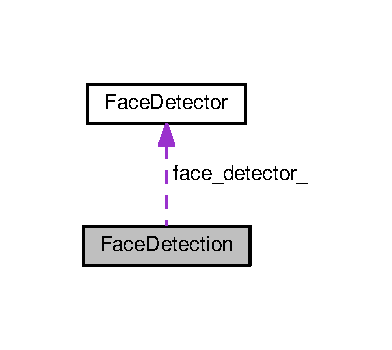
\includegraphics[width=188pt]{classFaceDetection__coll__graph}
\end{center}
\end{figure}
\subsection*{Public Member Functions}
\begin{DoxyCompactItemize}
\item 
\hyperlink{classFaceDetection_ae047cd60fcdc6a2b0fbfd06410c38529}{Face\-Detection} (void)
\begin{DoxyCompactList}\small\item\em Default constructor. \end{DoxyCompactList}\item 
bool \hyperlink{classFaceDetection_a72f1e1890fcf06eae61016ad42506314}{face\-Detection\-Callback} (rapp\-\_\-platform\-\_\-ros\-\_\-communications\-::\-Face\-Detection\-Ros\-Srv\-::\-Request \&req, rapp\-\_\-platform\-\_\-ros\-\_\-communications\-::\-Face\-Detection\-Ros\-Srv\-::\-Response \&res)
\begin{DoxyCompactList}\small\item\em Serves the face detection R\-O\-S service callback. \end{DoxyCompactList}\end{DoxyCompactItemize}
\subsection*{Private Attributes}
\begin{DoxyCompactItemize}
\item 
\hyperlink{classFaceDetector}{Face\-Detector} \hyperlink{classFaceDetection_a74003a22de1b6d9b1140f3e2c1a6444c}{face\-\_\-detector\-\_\-}
\item 
ros\-::\-Service\-Server \hyperlink{classFaceDetection_a72874127ac52787483a3f1a744771eb7}{face\-Detection\-Service\-\_\-}
\item 
std\-::string \hyperlink{classFaceDetection_a579ac45aa616167d12e25b7657c05af1}{face\-Detection\-Topic\-\_\-}
\item 
ros\-::\-Node\-Handle \hyperlink{classFaceDetection_a72f7ce4daf0768075f88c48db5957195}{nh\-\_\-}
\end{DoxyCompactItemize}


\subsection{Detailed Description}
Class \hyperlink{classFaceDetection}{Face\-Detection} uptakes the task of handling the R\-O\-S service callbacks. 

Definition at line 31 of file face\-\_\-detection.\-h.



\subsection{Constructor \& Destructor Documentation}
\hypertarget{classFaceDetection_ae047cd60fcdc6a2b0fbfd06410c38529}{\index{Face\-Detection@{Face\-Detection}!Face\-Detection@{Face\-Detection}}
\index{Face\-Detection@{Face\-Detection}!FaceDetection@{Face\-Detection}}
\subsubsection[{Face\-Detection}]{\setlength{\rightskip}{0pt plus 5cm}Face\-Detection\-::\-Face\-Detection (
\begin{DoxyParamCaption}
\item[{void}]{}
\end{DoxyParamCaption}
)}}\label{classFaceDetection_ae047cd60fcdc6a2b0fbfd06410c38529}


Default constructor. 

Default constructor. Performs initializations. 

Definition at line 24 of file face\-\_\-detection.\-cpp.



\subsection{Member Function Documentation}
\hypertarget{classFaceDetection_a72f1e1890fcf06eae61016ad42506314}{\index{Face\-Detection@{Face\-Detection}!face\-Detection\-Callback@{face\-Detection\-Callback}}
\index{face\-Detection\-Callback@{face\-Detection\-Callback}!FaceDetection@{Face\-Detection}}
\subsubsection[{face\-Detection\-Callback}]{\setlength{\rightskip}{0pt plus 5cm}bool Face\-Detection\-::face\-Detection\-Callback (
\begin{DoxyParamCaption}
\item[{rapp\-\_\-platform\-\_\-ros\-\_\-communications\-::\-Face\-Detection\-Ros\-Srv\-::\-Request \&}]{req, }
\item[{rapp\-\_\-platform\-\_\-ros\-\_\-communications\-::\-Face\-Detection\-Ros\-Srv\-::\-Response \&}]{res}
\end{DoxyParamCaption}
)}}\label{classFaceDetection_a72f1e1890fcf06eae61016ad42506314}


Serves the face detection R\-O\-S service callback. 


\begin{DoxyParams}{Parameters}
{\em req} & \mbox{[}rapp\-\_\-platform\-\_\-ros\-\_\-communications\-::\-Face\-Detection\-Ros\-Srv\-::\-Request\&\mbox{]} The R\-O\-S service request \\
\hline
{\em res} & \mbox{[}rapp\-\_\-platform\-\_\-ros\-\_\-communications\-::\-Face\-Detection\-Ros\-Srv\-::\-Response\&\mbox{]} The R\-O\-S service response \\
\hline
\end{DoxyParams}
\begin{DoxyReturn}{Returns}
bool -\/ The success status of the call 
\end{DoxyReturn}


Definition at line 42 of file face\-\_\-detection.\-cpp.



\subsection{Member Data Documentation}
\hypertarget{classFaceDetection_a74003a22de1b6d9b1140f3e2c1a6444c}{\index{Face\-Detection@{Face\-Detection}!face\-\_\-detector\-\_\-@{face\-\_\-detector\-\_\-}}
\index{face\-\_\-detector\-\_\-@{face\-\_\-detector\-\_\-}!FaceDetection@{Face\-Detection}}
\subsubsection[{face\-\_\-detector\-\_\-}]{\setlength{\rightskip}{0pt plus 5cm}{\bf Face\-Detector} Face\-Detection\-::face\-\_\-detector\-\_\-\hspace{0.3cm}{\ttfamily [private]}}}\label{classFaceDetection_a74003a22de1b6d9b1140f3e2c1a6444c}


Definition at line 62 of file face\-\_\-detection.\-h.

\hypertarget{classFaceDetection_a72874127ac52787483a3f1a744771eb7}{\index{Face\-Detection@{Face\-Detection}!face\-Detection\-Service\-\_\-@{face\-Detection\-Service\-\_\-}}
\index{face\-Detection\-Service\-\_\-@{face\-Detection\-Service\-\_\-}!FaceDetection@{Face\-Detection}}
\subsubsection[{face\-Detection\-Service\-\_\-}]{\setlength{\rightskip}{0pt plus 5cm}ros\-::\-Service\-Server Face\-Detection\-::face\-Detection\-Service\-\_\-\hspace{0.3cm}{\ttfamily [private]}}}\label{classFaceDetection_a72874127ac52787483a3f1a744771eb7}
Member variable holding the face detection R\-O\-S service topic 

Definition at line 56 of file face\-\_\-detection.\-h.

\hypertarget{classFaceDetection_a579ac45aa616167d12e25b7657c05af1}{\index{Face\-Detection@{Face\-Detection}!face\-Detection\-Topic\-\_\-@{face\-Detection\-Topic\-\_\-}}
\index{face\-Detection\-Topic\-\_\-@{face\-Detection\-Topic\-\_\-}!FaceDetection@{Face\-Detection}}
\subsubsection[{face\-Detection\-Topic\-\_\-}]{\setlength{\rightskip}{0pt plus 5cm}std\-::string Face\-Detection\-::face\-Detection\-Topic\-\_\-\hspace{0.3cm}{\ttfamily [private]}}}\label{classFaceDetection_a579ac45aa616167d12e25b7657c05af1}
Object of type \hyperlink{classFaceDetector}{Face\-Detector} 

Definition at line 59 of file face\-\_\-detection.\-h.

\hypertarget{classFaceDetection_a72f7ce4daf0768075f88c48db5957195}{\index{Face\-Detection@{Face\-Detection}!nh\-\_\-@{nh\-\_\-}}
\index{nh\-\_\-@{nh\-\_\-}!FaceDetection@{Face\-Detection}}
\subsubsection[{nh\-\_\-}]{\setlength{\rightskip}{0pt plus 5cm}ros\-::\-Node\-Handle Face\-Detection\-::nh\-\_\-\hspace{0.3cm}{\ttfamily [private]}}}\label{classFaceDetection_a72f7ce4daf0768075f88c48db5957195}
$<$ The R\-O\-S node handle The face detection service server 

Definition at line 53 of file face\-\_\-detection.\-h.



The documentation for this class was generated from the following files\-:\begin{DoxyCompactItemize}
\item 
/home/travis/rapp\-\_\-temp/rapp-\/platform/rapp\-\_\-face\-\_\-detection/include/face\-\_\-detection/\hyperlink{face__detection_8h}{face\-\_\-detection.\-h}\item 
/home/travis/rapp\-\_\-temp/rapp-\/platform/rapp\-\_\-face\-\_\-detection/src/\hyperlink{face__detection_8cpp}{face\-\_\-detection.\-cpp}\end{DoxyCompactItemize}

\hypertarget{classFaceDetector}{\section{Face\-Detector Class Reference}
\label{classFaceDetector}\index{Face\-Detector@{Face\-Detector}}
}


Class that implements a face detection algorithm based on a Haar cascade classifier.  




{\ttfamily \#include $<$face\-\_\-detector.\-h$>$}

\subsection*{Public Member Functions}
\begin{DoxyCompactItemize}
\item 
\hyperlink{classFaceDetector_af08a8c38a26b029e02e05d8d9498332c}{Face\-Detector} (void)
\begin{DoxyCompactList}\small\item\em Default constructor. \end{DoxyCompactList}\item 
std\-::vector$<$ cv\-::\-Rect $>$ \hyperlink{classFaceDetector_a154988581f876e3a15f59c57c4420df8}{detect\-Faces} (const cv\-::\-Mat \&input\-\_\-img, bool fast=false)
\begin{DoxyCompactList}\small\item\em Detects faces from a cv\-::\-Mat. \end{DoxyCompactList}\item 
std\-::vector$<$ cv\-::\-Rect $>$ \hyperlink{classFaceDetector_a590b5ba361a049b2b93d63ebb7518647}{find\-Faces} (std\-::string file\-\_\-name, bool fast=false)
\begin{DoxyCompactList}\small\item\em Finds faces in an image retrieved from a file U\-R\-L. \end{DoxyCompactList}\item 
cv\-::\-Mat \hyperlink{classFaceDetector_ad8223498ebc15a177485f86274583d81}{load\-Image} (std\-::string file\-\_\-name)
\begin{DoxyCompactList}\small\item\em Loads an image from a file U\-R\-L. \end{DoxyCompactList}\end{DoxyCompactItemize}
\subsection*{Private Member Functions}
\begin{DoxyCompactItemize}
\item 
std\-::vector$<$ cv\-::\-Rect $>$ \hyperlink{classFaceDetector_a442209589a939c663ed1ab07dd6c3a90}{detect\-Faces} (const cv\-::\-Mat \&input\-\_\-img, const std\-::string \&haar\-\_\-path)
\begin{DoxyCompactList}\small\item\em Detects faces from a cv\-::\-Mat. \end{DoxyCompactList}\item 
std\-::vector$<$ cv\-::\-Rect $>$ \hyperlink{classFaceDetector_a31426b2557e0548c5ca5c0542e51f394}{identify\-Unique\-Faces} (const std\-::vector$<$ cv\-::\-Rect $>$ first\-Face\-Vector, const std\-::vector$<$ cv\-::\-Rect $>$ second\-Face\-Vector)
\begin{DoxyCompactList}\small\item\em Identify unique faces from two sets of faces. \end{DoxyCompactList}\end{DoxyCompactItemize}


\subsection{Detailed Description}
Class that implements a face detection algorithm based on a Haar cascade classifier. 

Definition at line 33 of file face\-\_\-detector.\-h.



\subsection{Constructor \& Destructor Documentation}
\hypertarget{classFaceDetector_af08a8c38a26b029e02e05d8d9498332c}{\index{Face\-Detector@{Face\-Detector}!Face\-Detector@{Face\-Detector}}
\index{Face\-Detector@{Face\-Detector}!FaceDetector@{Face\-Detector}}
\subsubsection[{Face\-Detector}]{\setlength{\rightskip}{0pt plus 5cm}Face\-Detector\-::\-Face\-Detector (
\begin{DoxyParamCaption}
\item[{void}]{}
\end{DoxyParamCaption}
)}}\label{classFaceDetector_af08a8c38a26b029e02e05d8d9498332c}


Default constructor. 



Definition at line 26 of file face\-\_\-detector.\-cpp.



\subsection{Member Function Documentation}
\hypertarget{classFaceDetector_a154988581f876e3a15f59c57c4420df8}{\index{Face\-Detector@{Face\-Detector}!detect\-Faces@{detect\-Faces}}
\index{detect\-Faces@{detect\-Faces}!FaceDetector@{Face\-Detector}}
\subsubsection[{detect\-Faces}]{\setlength{\rightskip}{0pt plus 5cm}std\-::vector$<$ cv\-::\-Rect $>$ Face\-Detector\-::detect\-Faces (
\begin{DoxyParamCaption}
\item[{const cv\-::\-Mat \&}]{input\-\_\-img, }
\item[{bool}]{fast = {\ttfamily false}}
\end{DoxyParamCaption}
)}}\label{classFaceDetector_a154988581f876e3a15f59c57c4420df8}


Detects faces from a cv\-::\-Mat. 


\begin{DoxyParams}{Parameters}
{\em input\-\_\-img} & \mbox{[}const cv\-::\-Mat\&\mbox{]} The input image \\
\hline
{\em fast} & \mbox{[}bool\mbox{]} True for fast detection -- frontal only \\
\hline
\end{DoxyParams}
\begin{DoxyReturn}{Returns}
\mbox{[}std\-::vector$<$cv\-::\-Rect$>$\mbox{]} A vector containing the detected faces. Each face is represented by a rectangle. 
\end{DoxyReturn}


Definition at line 50 of file face\-\_\-detector.\-cpp.

\hypertarget{classFaceDetector_a442209589a939c663ed1ab07dd6c3a90}{\index{Face\-Detector@{Face\-Detector}!detect\-Faces@{detect\-Faces}}
\index{detect\-Faces@{detect\-Faces}!FaceDetector@{Face\-Detector}}
\subsubsection[{detect\-Faces}]{\setlength{\rightskip}{0pt plus 5cm}std\-::vector$<$ cv\-::\-Rect $>$ Face\-Detector\-::detect\-Faces (
\begin{DoxyParamCaption}
\item[{const cv\-::\-Mat \&}]{input\-\_\-img, }
\item[{const std\-::string \&}]{haar\-\_\-path}
\end{DoxyParamCaption}
)\hspace{0.3cm}{\ttfamily [private]}}}\label{classFaceDetector_a442209589a939c663ed1ab07dd6c3a90}


Detects faces from a cv\-::\-Mat. 


\begin{DoxyParams}{Parameters}
{\em input\-\_\-img} & \mbox{[}const cv\-::\-Mat\&\mbox{]} The input image \\
\hline
{\em haar\-\_\-path} & \mbox{[}const std\-::string\mbox{]} The Haar training model path \\
\hline
\end{DoxyParams}
\begin{DoxyReturn}{Returns}
\mbox{[}std\-::vector$<$cv\-::\-Rect$>$\mbox{]} A vector containing the detected faces. Each face is represented by a rectangle. 
\end{DoxyReturn}


Definition at line 89 of file face\-\_\-detector.\-cpp.

\hypertarget{classFaceDetector_a590b5ba361a049b2b93d63ebb7518647}{\index{Face\-Detector@{Face\-Detector}!find\-Faces@{find\-Faces}}
\index{find\-Faces@{find\-Faces}!FaceDetector@{Face\-Detector}}
\subsubsection[{find\-Faces}]{\setlength{\rightskip}{0pt plus 5cm}std\-::vector$<$ cv\-::\-Rect $>$ Face\-Detector\-::find\-Faces (
\begin{DoxyParamCaption}
\item[{std\-::string}]{file\-\_\-name, }
\item[{bool}]{fast = {\ttfamily false}}
\end{DoxyParamCaption}
)}}\label{classFaceDetector_a590b5ba361a049b2b93d63ebb7518647}


Finds faces in an image retrieved from a file U\-R\-L. 


\begin{DoxyParams}{Parameters}
{\em file\-\_\-name} & \mbox{[}std\-::string\mbox{]} The image file's U\-R\-L \\
\hline
{\em fast} & \mbox{[}bool\mbox{]} True for fast detection -- frontal only \\
\hline
\end{DoxyParams}
\begin{DoxyReturn}{Returns}
\mbox{[}std\-::vector$<$cv\-::\-Rect$>$\mbox{]} A vector containing the detected faces. Each face is represented by a rectangle. 
\end{DoxyReturn}


Definition at line 168 of file face\-\_\-detector.\-cpp.

\hypertarget{classFaceDetector_a31426b2557e0548c5ca5c0542e51f394}{\index{Face\-Detector@{Face\-Detector}!identify\-Unique\-Faces@{identify\-Unique\-Faces}}
\index{identify\-Unique\-Faces@{identify\-Unique\-Faces}!FaceDetector@{Face\-Detector}}
\subsubsection[{identify\-Unique\-Faces}]{\setlength{\rightskip}{0pt plus 5cm}std\-::vector$<$ cv\-::\-Rect $>$ Face\-Detector\-::identify\-Unique\-Faces (
\begin{DoxyParamCaption}
\item[{const std\-::vector$<$ cv\-::\-Rect $>$}]{first\-Face\-Vector, }
\item[{const std\-::vector$<$ cv\-::\-Rect $>$}]{second\-Face\-Vector}
\end{DoxyParamCaption}
)\hspace{0.3cm}{\ttfamily [private]}}}\label{classFaceDetector_a31426b2557e0548c5ca5c0542e51f394}


Identify unique faces from two sets of faces. 


\begin{DoxyParams}{Parameters}
{\em front\-Face\-Vector} & \mbox{[}const std\-::vector$<$cv\-::\-Rect$>$\&\mbox{]} The first set of faces \\
\hline
{\em second\-Face\-Vector} & \mbox{[}const std\-::vector$<$cv\-::\-Rect$>$\&\mbox{]} The second set of faces \\
\hline
\end{DoxyParams}
\begin{DoxyReturn}{Returns}
\mbox{[}std\-::vector$<$cv\-::\-Rect$>$\mbox{]} A vector containing the unique faces. Each face is represented by a rectangle. 
\end{DoxyReturn}


Definition at line 140 of file face\-\_\-detector.\-cpp.

\hypertarget{classFaceDetector_ad8223498ebc15a177485f86274583d81}{\index{Face\-Detector@{Face\-Detector}!load\-Image@{load\-Image}}
\index{load\-Image@{load\-Image}!FaceDetector@{Face\-Detector}}
\subsubsection[{load\-Image}]{\setlength{\rightskip}{0pt plus 5cm}cv\-::\-Mat Face\-Detector\-::load\-Image (
\begin{DoxyParamCaption}
\item[{std\-::string}]{file\-\_\-name}
\end{DoxyParamCaption}
)}}\label{classFaceDetector_ad8223498ebc15a177485f86274583d81}


Loads an image from a file U\-R\-L. 


\begin{DoxyParams}{Parameters}
{\em file\-\_\-name} & \mbox{[}std\-::string\mbox{]} The image's file U\-R\-L \\
\hline
\end{DoxyParams}
\begin{DoxyReturn}{Returns}
\mbox{[}cv\-::\-Mat\mbox{]} The image in Open\-C\-V representation 
\end{DoxyReturn}


Definition at line 35 of file face\-\_\-detector.\-cpp.



The documentation for this class was generated from the following files\-:\begin{DoxyCompactItemize}
\item 
/home/travis/rapp\-\_\-temp/rapp-\/platform/rapp\-\_\-face\-\_\-detection/include/face\-\_\-detection/\hyperlink{face__detector_8h}{face\-\_\-detector.\-h}\item 
/home/travis/rapp\-\_\-temp/rapp-\/platform/rapp\-\_\-face\-\_\-detection/src/\hyperlink{face__detector_8cpp}{face\-\_\-detector.\-cpp}\end{DoxyCompactItemize}

\hypertarget{classrapp__speech__detection__sphinx4_1_1global__parameters_1_1GlobalParams}{\section{rapp\-\_\-speech\-\_\-detection\-\_\-sphinx4.\-global\-\_\-parameters.\-Global\-Params Class Reference}
\label{classrapp__speech__detection__sphinx4_1_1global__parameters_1_1GlobalParams}\index{rapp\-\_\-speech\-\_\-detection\-\_\-sphinx4.\-global\-\_\-parameters.\-Global\-Params@{rapp\-\_\-speech\-\_\-detection\-\_\-sphinx4.\-global\-\_\-parameters.\-Global\-Params}}
}


Contains global Sphinx parameters.  


\subsection*{Public Member Functions}
\begin{DoxyCompactItemize}
\item 
def \hyperlink{classrapp__speech__detection__sphinx4_1_1global__parameters_1_1GlobalParams_a00ffd74720678058d8380021d4a167d9}{\-\_\-\-\_\-init\-\_\-\-\_\-}
\end{DoxyCompactItemize}
\subsection*{Public Attributes}
\begin{DoxyCompactItemize}
\item 
\hyperlink{classrapp__speech__detection__sphinx4_1_1global__parameters_1_1GlobalParams_a544bff3ab91e6ec8c782ba2b4386ef0a}{rospack}
\end{DoxyCompactItemize}
\subsection*{Private Attributes}
\begin{DoxyCompactItemize}
\item 
\hyperlink{classrapp__speech__detection__sphinx4_1_1global__parameters_1_1GlobalParams_a21df0be4b855b05285c4dc7d35d7454f}{\-\_\-acoustic\-\_\-models\-\_\-url}
\begin{DoxyCompactList}\small\item\em Acoustic models path. \end{DoxyCompactList}\item 
\hyperlink{classrapp__speech__detection__sphinx4_1_1global__parameters_1_1GlobalParams_a401cee442875d271a64c6cff9eb376ed}{\-\_\-allow\-\_\-sphinx\-\_\-output}
\begin{DoxyCompactList}\small\item\em True if Sphinx is allowed output on S\-T\-D\-I\-N, S\-T\-D\-E\-R\-R. \end{DoxyCompactList}\item 
\hyperlink{classrapp__speech__detection__sphinx4_1_1global__parameters_1_1GlobalParams_a669e25ce189ad6cae67f52ebeb3404c7}{\-\_\-language\-\_\-models\-\_\-url}
\begin{DoxyCompactList}\small\item\em Language models path. \end{DoxyCompactList}\item 
\hyperlink{classrapp__speech__detection__sphinx4_1_1global__parameters_1_1GlobalParams_a254c79291b9c78ea0a08b86accdcf3d0}{\-\_\-noise\-\_\-profiles\-\_\-url}
\begin{DoxyCompactList}\small\item\em Noise profiles path. \end{DoxyCompactList}\item 
\hyperlink{classrapp__speech__detection__sphinx4_1_1global__parameters_1_1GlobalParams_a3f81e8f790adf1b6e8de24b8aaa5d7a3}{\-\_\-socket\-\_\-host}
\begin{DoxyCompactList}\small\item\em I\-P\-C socket H\-O\-S\-T parameter. \end{DoxyCompactList}\item 
\hyperlink{classrapp__speech__detection__sphinx4_1_1global__parameters_1_1GlobalParams_aef8bca74a5ed8b58dbe8f842c3e685e0}{\-\_\-sphinx\-\_\-jar\-\_\-file}
\begin{DoxyCompactList}\small\item\em Sphinx jar file path. \end{DoxyCompactList}\item 
\hyperlink{classrapp__speech__detection__sphinx4_1_1global__parameters_1_1GlobalParams_afcb09126b08bb8de186f3687f62ff83a}{\-\_\-sphinx\-\_\-jar\-\_\-files\-\_\-url}
\begin{DoxyCompactList}\small\item\em Java libraries path. \end{DoxyCompactList}\item 
\hyperlink{classrapp__speech__detection__sphinx4_1_1global__parameters_1_1GlobalParams_aec2fabfa84128e000d5af362d659cc95}{\-\_\-sphinx\-\_\-package\-\_\-url}
\begin{DoxyCompactList}\small\item\em Sphinx package path. \end{DoxyCompactList}\item 
\hyperlink{classrapp__speech__detection__sphinx4_1_1global__parameters_1_1GlobalParams_a7812512e88ceff516022a250a218a7c6}{\-\_\-sphinx\-\_\-preconf}
\begin{DoxyCompactList}\small\item\em Sphinx preconfigurations yaml. \end{DoxyCompactList}\item 
\hyperlink{classrapp__speech__detection__sphinx4_1_1global__parameters_1_1GlobalParams_ac21cbb95712d8873cf5c357e7006bf59}{\-\_\-tmp\-\_\-language\-\_\-models\-\_\-url}
\begin{DoxyCompactList}\small\item\em Temporary language models path. \end{DoxyCompactList}\end{DoxyCompactItemize}


\subsection{Detailed Description}
Contains global Sphinx parameters. 

Definition at line 22 of file global\-\_\-parameters.\-py.



\subsection{Constructor \& Destructor Documentation}
\hypertarget{classrapp__speech__detection__sphinx4_1_1global__parameters_1_1GlobalParams_a00ffd74720678058d8380021d4a167d9}{\index{rapp\-\_\-speech\-\_\-detection\-\_\-sphinx4\-::global\-\_\-parameters\-::\-Global\-Params@{rapp\-\_\-speech\-\_\-detection\-\_\-sphinx4\-::global\-\_\-parameters\-::\-Global\-Params}!\-\_\-\-\_\-init\-\_\-\-\_\-@{\-\_\-\-\_\-init\-\_\-\-\_\-}}
\index{\-\_\-\-\_\-init\-\_\-\-\_\-@{\-\_\-\-\_\-init\-\_\-\-\_\-}!rapp_speech_detection_sphinx4::global_parameters::GlobalParams@{rapp\-\_\-speech\-\_\-detection\-\_\-sphinx4\-::global\-\_\-parameters\-::\-Global\-Params}}
\subsubsection[{\-\_\-\-\_\-init\-\_\-\-\_\-}]{\setlength{\rightskip}{0pt plus 5cm}def rapp\-\_\-speech\-\_\-detection\-\_\-sphinx4.\-global\-\_\-parameters.\-Global\-Params.\-\_\-\-\_\-init\-\_\-\-\_\- (
\begin{DoxyParamCaption}
\item[{}]{self}
\end{DoxyParamCaption}
)}}\label{classrapp__speech__detection__sphinx4_1_1global__parameters_1_1GlobalParams_a00ffd74720678058d8380021d4a167d9}


Definition at line 23 of file global\-\_\-parameters.\-py.



\subsection{Member Data Documentation}
\hypertarget{classrapp__speech__detection__sphinx4_1_1global__parameters_1_1GlobalParams_a21df0be4b855b05285c4dc7d35d7454f}{\index{rapp\-\_\-speech\-\_\-detection\-\_\-sphinx4\-::global\-\_\-parameters\-::\-Global\-Params@{rapp\-\_\-speech\-\_\-detection\-\_\-sphinx4\-::global\-\_\-parameters\-::\-Global\-Params}!\-\_\-acoustic\-\_\-models\-\_\-url@{\-\_\-acoustic\-\_\-models\-\_\-url}}
\index{\-\_\-acoustic\-\_\-models\-\_\-url@{\-\_\-acoustic\-\_\-models\-\_\-url}!rapp_speech_detection_sphinx4::global_parameters::GlobalParams@{rapp\-\_\-speech\-\_\-detection\-\_\-sphinx4\-::global\-\_\-parameters\-::\-Global\-Params}}
\subsubsection[{\-\_\-acoustic\-\_\-models\-\_\-url}]{\setlength{\rightskip}{0pt plus 5cm}rapp\-\_\-speech\-\_\-detection\-\_\-sphinx4.\-global\-\_\-parameters.\-Global\-Params.\-\_\-acoustic\-\_\-models\-\_\-url\hspace{0.3cm}{\ttfamily [private]}}}\label{classrapp__speech__detection__sphinx4_1_1global__parameters_1_1GlobalParams_a21df0be4b855b05285c4dc7d35d7454f}


Acoustic models path. 



Definition at line 38 of file global\-\_\-parameters.\-py.

\hypertarget{classrapp__speech__detection__sphinx4_1_1global__parameters_1_1GlobalParams_a401cee442875d271a64c6cff9eb376ed}{\index{rapp\-\_\-speech\-\_\-detection\-\_\-sphinx4\-::global\-\_\-parameters\-::\-Global\-Params@{rapp\-\_\-speech\-\_\-detection\-\_\-sphinx4\-::global\-\_\-parameters\-::\-Global\-Params}!\-\_\-allow\-\_\-sphinx\-\_\-output@{\-\_\-allow\-\_\-sphinx\-\_\-output}}
\index{\-\_\-allow\-\_\-sphinx\-\_\-output@{\-\_\-allow\-\_\-sphinx\-\_\-output}!rapp_speech_detection_sphinx4::global_parameters::GlobalParams@{rapp\-\_\-speech\-\_\-detection\-\_\-sphinx4\-::global\-\_\-parameters\-::\-Global\-Params}}
\subsubsection[{\-\_\-allow\-\_\-sphinx\-\_\-output}]{\setlength{\rightskip}{0pt plus 5cm}rapp\-\_\-speech\-\_\-detection\-\_\-sphinx4.\-global\-\_\-parameters.\-Global\-Params.\-\_\-allow\-\_\-sphinx\-\_\-output\hspace{0.3cm}{\ttfamily [private]}}}\label{classrapp__speech__detection__sphinx4_1_1global__parameters_1_1GlobalParams_a401cee442875d271a64c6cff9eb376ed}


True if Sphinx is allowed output on S\-T\-D\-I\-N, S\-T\-D\-E\-R\-R. 



Definition at line 43 of file global\-\_\-parameters.\-py.

\hypertarget{classrapp__speech__detection__sphinx4_1_1global__parameters_1_1GlobalParams_a669e25ce189ad6cae67f52ebeb3404c7}{\index{rapp\-\_\-speech\-\_\-detection\-\_\-sphinx4\-::global\-\_\-parameters\-::\-Global\-Params@{rapp\-\_\-speech\-\_\-detection\-\_\-sphinx4\-::global\-\_\-parameters\-::\-Global\-Params}!\-\_\-language\-\_\-models\-\_\-url@{\-\_\-language\-\_\-models\-\_\-url}}
\index{\-\_\-language\-\_\-models\-\_\-url@{\-\_\-language\-\_\-models\-\_\-url}!rapp_speech_detection_sphinx4::global_parameters::GlobalParams@{rapp\-\_\-speech\-\_\-detection\-\_\-sphinx4\-::global\-\_\-parameters\-::\-Global\-Params}}
\subsubsection[{\-\_\-language\-\_\-models\-\_\-url}]{\setlength{\rightskip}{0pt plus 5cm}rapp\-\_\-speech\-\_\-detection\-\_\-sphinx4.\-global\-\_\-parameters.\-Global\-Params.\-\_\-language\-\_\-models\-\_\-url\hspace{0.3cm}{\ttfamily [private]}}}\label{classrapp__speech__detection__sphinx4_1_1global__parameters_1_1GlobalParams_a669e25ce189ad6cae67f52ebeb3404c7}


Language models path. 



Definition at line 31 of file global\-\_\-parameters.\-py.

\hypertarget{classrapp__speech__detection__sphinx4_1_1global__parameters_1_1GlobalParams_a254c79291b9c78ea0a08b86accdcf3d0}{\index{rapp\-\_\-speech\-\_\-detection\-\_\-sphinx4\-::global\-\_\-parameters\-::\-Global\-Params@{rapp\-\_\-speech\-\_\-detection\-\_\-sphinx4\-::global\-\_\-parameters\-::\-Global\-Params}!\-\_\-noise\-\_\-profiles\-\_\-url@{\-\_\-noise\-\_\-profiles\-\_\-url}}
\index{\-\_\-noise\-\_\-profiles\-\_\-url@{\-\_\-noise\-\_\-profiles\-\_\-url}!rapp_speech_detection_sphinx4::global_parameters::GlobalParams@{rapp\-\_\-speech\-\_\-detection\-\_\-sphinx4\-::global\-\_\-parameters\-::\-Global\-Params}}
\subsubsection[{\-\_\-noise\-\_\-profiles\-\_\-url}]{\setlength{\rightskip}{0pt plus 5cm}rapp\-\_\-speech\-\_\-detection\-\_\-sphinx4.\-global\-\_\-parameters.\-Global\-Params.\-\_\-noise\-\_\-profiles\-\_\-url\hspace{0.3cm}{\ttfamily [private]}}}\label{classrapp__speech__detection__sphinx4_1_1global__parameters_1_1GlobalParams_a254c79291b9c78ea0a08b86accdcf3d0}


Noise profiles path. 



Definition at line 36 of file global\-\_\-parameters.\-py.

\hypertarget{classrapp__speech__detection__sphinx4_1_1global__parameters_1_1GlobalParams_a3f81e8f790adf1b6e8de24b8aaa5d7a3}{\index{rapp\-\_\-speech\-\_\-detection\-\_\-sphinx4\-::global\-\_\-parameters\-::\-Global\-Params@{rapp\-\_\-speech\-\_\-detection\-\_\-sphinx4\-::global\-\_\-parameters\-::\-Global\-Params}!\-\_\-socket\-\_\-host@{\-\_\-socket\-\_\-host}}
\index{\-\_\-socket\-\_\-host@{\-\_\-socket\-\_\-host}!rapp_speech_detection_sphinx4::global_parameters::GlobalParams@{rapp\-\_\-speech\-\_\-detection\-\_\-sphinx4\-::global\-\_\-parameters\-::\-Global\-Params}}
\subsubsection[{\-\_\-socket\-\_\-host}]{\setlength{\rightskip}{0pt plus 5cm}rapp\-\_\-speech\-\_\-detection\-\_\-sphinx4.\-global\-\_\-parameters.\-Global\-Params.\-\_\-socket\-\_\-host\hspace{0.3cm}{\ttfamily [private]}}}\label{classrapp__speech__detection__sphinx4_1_1global__parameters_1_1GlobalParams_a3f81e8f790adf1b6e8de24b8aaa5d7a3}


I\-P\-C socket H\-O\-S\-T parameter. 



Definition at line 45 of file global\-\_\-parameters.\-py.

\hypertarget{classrapp__speech__detection__sphinx4_1_1global__parameters_1_1GlobalParams_aef8bca74a5ed8b58dbe8f842c3e685e0}{\index{rapp\-\_\-speech\-\_\-detection\-\_\-sphinx4\-::global\-\_\-parameters\-::\-Global\-Params@{rapp\-\_\-speech\-\_\-detection\-\_\-sphinx4\-::global\-\_\-parameters\-::\-Global\-Params}!\-\_\-sphinx\-\_\-jar\-\_\-file@{\-\_\-sphinx\-\_\-jar\-\_\-file}}
\index{\-\_\-sphinx\-\_\-jar\-\_\-file@{\-\_\-sphinx\-\_\-jar\-\_\-file}!rapp_speech_detection_sphinx4::global_parameters::GlobalParams@{rapp\-\_\-speech\-\_\-detection\-\_\-sphinx4\-::global\-\_\-parameters\-::\-Global\-Params}}
\subsubsection[{\-\_\-sphinx\-\_\-jar\-\_\-file}]{\setlength{\rightskip}{0pt plus 5cm}rapp\-\_\-speech\-\_\-detection\-\_\-sphinx4.\-global\-\_\-parameters.\-Global\-Params.\-\_\-sphinx\-\_\-jar\-\_\-file\hspace{0.3cm}{\ttfamily [private]}}}\label{classrapp__speech__detection__sphinx4_1_1global__parameters_1_1GlobalParams_aef8bca74a5ed8b58dbe8f842c3e685e0}


Sphinx jar file path. 



Definition at line 41 of file global\-\_\-parameters.\-py.

\hypertarget{classrapp__speech__detection__sphinx4_1_1global__parameters_1_1GlobalParams_afcb09126b08bb8de186f3687f62ff83a}{\index{rapp\-\_\-speech\-\_\-detection\-\_\-sphinx4\-::global\-\_\-parameters\-::\-Global\-Params@{rapp\-\_\-speech\-\_\-detection\-\_\-sphinx4\-::global\-\_\-parameters\-::\-Global\-Params}!\-\_\-sphinx\-\_\-jar\-\_\-files\-\_\-url@{\-\_\-sphinx\-\_\-jar\-\_\-files\-\_\-url}}
\index{\-\_\-sphinx\-\_\-jar\-\_\-files\-\_\-url@{\-\_\-sphinx\-\_\-jar\-\_\-files\-\_\-url}!rapp_speech_detection_sphinx4::global_parameters::GlobalParams@{rapp\-\_\-speech\-\_\-detection\-\_\-sphinx4\-::global\-\_\-parameters\-::\-Global\-Params}}
\subsubsection[{\-\_\-sphinx\-\_\-jar\-\_\-files\-\_\-url}]{\setlength{\rightskip}{0pt plus 5cm}rapp\-\_\-speech\-\_\-detection\-\_\-sphinx4.\-global\-\_\-parameters.\-Global\-Params.\-\_\-sphinx\-\_\-jar\-\_\-files\-\_\-url\hspace{0.3cm}{\ttfamily [private]}}}\label{classrapp__speech__detection__sphinx4_1_1global__parameters_1_1GlobalParams_afcb09126b08bb8de186f3687f62ff83a}


Java libraries path. 



Definition at line 27 of file global\-\_\-parameters.\-py.

\hypertarget{classrapp__speech__detection__sphinx4_1_1global__parameters_1_1GlobalParams_aec2fabfa84128e000d5af362d659cc95}{\index{rapp\-\_\-speech\-\_\-detection\-\_\-sphinx4\-::global\-\_\-parameters\-::\-Global\-Params@{rapp\-\_\-speech\-\_\-detection\-\_\-sphinx4\-::global\-\_\-parameters\-::\-Global\-Params}!\-\_\-sphinx\-\_\-package\-\_\-url@{\-\_\-sphinx\-\_\-package\-\_\-url}}
\index{\-\_\-sphinx\-\_\-package\-\_\-url@{\-\_\-sphinx\-\_\-package\-\_\-url}!rapp_speech_detection_sphinx4::global_parameters::GlobalParams@{rapp\-\_\-speech\-\_\-detection\-\_\-sphinx4\-::global\-\_\-parameters\-::\-Global\-Params}}
\subsubsection[{\-\_\-sphinx\-\_\-package\-\_\-url}]{\setlength{\rightskip}{0pt plus 5cm}rapp\-\_\-speech\-\_\-detection\-\_\-sphinx4.\-global\-\_\-parameters.\-Global\-Params.\-\_\-sphinx\-\_\-package\-\_\-url\hspace{0.3cm}{\ttfamily [private]}}}\label{classrapp__speech__detection__sphinx4_1_1global__parameters_1_1GlobalParams_aec2fabfa84128e000d5af362d659cc95}


Sphinx package path. 



Definition at line 29 of file global\-\_\-parameters.\-py.

\hypertarget{classrapp__speech__detection__sphinx4_1_1global__parameters_1_1GlobalParams_a7812512e88ceff516022a250a218a7c6}{\index{rapp\-\_\-speech\-\_\-detection\-\_\-sphinx4\-::global\-\_\-parameters\-::\-Global\-Params@{rapp\-\_\-speech\-\_\-detection\-\_\-sphinx4\-::global\-\_\-parameters\-::\-Global\-Params}!\-\_\-sphinx\-\_\-preconf@{\-\_\-sphinx\-\_\-preconf}}
\index{\-\_\-sphinx\-\_\-preconf@{\-\_\-sphinx\-\_\-preconf}!rapp_speech_detection_sphinx4::global_parameters::GlobalParams@{rapp\-\_\-speech\-\_\-detection\-\_\-sphinx4\-::global\-\_\-parameters\-::\-Global\-Params}}
\subsubsection[{\-\_\-sphinx\-\_\-preconf}]{\setlength{\rightskip}{0pt plus 5cm}rapp\-\_\-speech\-\_\-detection\-\_\-sphinx4.\-global\-\_\-parameters.\-Global\-Params.\-\_\-sphinx\-\_\-preconf\hspace{0.3cm}{\ttfamily [private]}}}\label{classrapp__speech__detection__sphinx4_1_1global__parameters_1_1GlobalParams_a7812512e88ceff516022a250a218a7c6}


Sphinx preconfigurations yaml. 



Definition at line 47 of file global\-\_\-parameters.\-py.

\hypertarget{classrapp__speech__detection__sphinx4_1_1global__parameters_1_1GlobalParams_ac21cbb95712d8873cf5c357e7006bf59}{\index{rapp\-\_\-speech\-\_\-detection\-\_\-sphinx4\-::global\-\_\-parameters\-::\-Global\-Params@{rapp\-\_\-speech\-\_\-detection\-\_\-sphinx4\-::global\-\_\-parameters\-::\-Global\-Params}!\-\_\-tmp\-\_\-language\-\_\-models\-\_\-url@{\-\_\-tmp\-\_\-language\-\_\-models\-\_\-url}}
\index{\-\_\-tmp\-\_\-language\-\_\-models\-\_\-url@{\-\_\-tmp\-\_\-language\-\_\-models\-\_\-url}!rapp_speech_detection_sphinx4::global_parameters::GlobalParams@{rapp\-\_\-speech\-\_\-detection\-\_\-sphinx4\-::global\-\_\-parameters\-::\-Global\-Params}}
\subsubsection[{\-\_\-tmp\-\_\-language\-\_\-models\-\_\-url}]{\setlength{\rightskip}{0pt plus 5cm}rapp\-\_\-speech\-\_\-detection\-\_\-sphinx4.\-global\-\_\-parameters.\-Global\-Params.\-\_\-tmp\-\_\-language\-\_\-models\-\_\-url\hspace{0.3cm}{\ttfamily [private]}}}\label{classrapp__speech__detection__sphinx4_1_1global__parameters_1_1GlobalParams_ac21cbb95712d8873cf5c357e7006bf59}


Temporary language models path. 



Definition at line 33 of file global\-\_\-parameters.\-py.

\hypertarget{classrapp__speech__detection__sphinx4_1_1global__parameters_1_1GlobalParams_a544bff3ab91e6ec8c782ba2b4386ef0a}{\index{rapp\-\_\-speech\-\_\-detection\-\_\-sphinx4\-::global\-\_\-parameters\-::\-Global\-Params@{rapp\-\_\-speech\-\_\-detection\-\_\-sphinx4\-::global\-\_\-parameters\-::\-Global\-Params}!rospack@{rospack}}
\index{rospack@{rospack}!rapp_speech_detection_sphinx4::global_parameters::GlobalParams@{rapp\-\_\-speech\-\_\-detection\-\_\-sphinx4\-::global\-\_\-parameters\-::\-Global\-Params}}
\subsubsection[{rospack}]{\setlength{\rightskip}{0pt plus 5cm}rapp\-\_\-speech\-\_\-detection\-\_\-sphinx4.\-global\-\_\-parameters.\-Global\-Params.\-rospack}}\label{classrapp__speech__detection__sphinx4_1_1global__parameters_1_1GlobalParams_a544bff3ab91e6ec8c782ba2b4386ef0a}


Definition at line 24 of file global\-\_\-parameters.\-py.



The documentation for this class was generated from the following file\-:\begin{DoxyCompactItemize}
\item 
/home/travis/rapp\-\_\-temp/rapp-\/platform/rapp\-\_\-speech\-\_\-detection\-\_\-sphinx4/src/rapp\-\_\-speech\-\_\-detection\-\_\-sphinx4/\hyperlink{global__parameters_8py}{global\-\_\-parameters.\-py}\end{DoxyCompactItemize}

\hypertarget{classrapp__speech__detection__sphinx4_1_1greek__support_1_1GreekSupport}{\section{rapp\-\_\-speech\-\_\-detection\-\_\-sphinx4.\-greek\-\_\-support.\-Greek\-Support Class Reference}
\label{classrapp__speech__detection__sphinx4_1_1greek__support_1_1GreekSupport}\index{rapp\-\_\-speech\-\_\-detection\-\_\-sphinx4.\-greek\-\_\-support.\-Greek\-Support@{rapp\-\_\-speech\-\_\-detection\-\_\-sphinx4.\-greek\-\_\-support.\-Greek\-Support}}
}


Allows the creation of configuration files for Greek Sphinx speech recognition.  




Inheritance diagram for rapp\-\_\-speech\-\_\-detection\-\_\-sphinx4.\-greek\-\_\-support.\-Greek\-Support\-:
\nopagebreak
\begin{figure}[H]
\begin{center}
\leavevmode
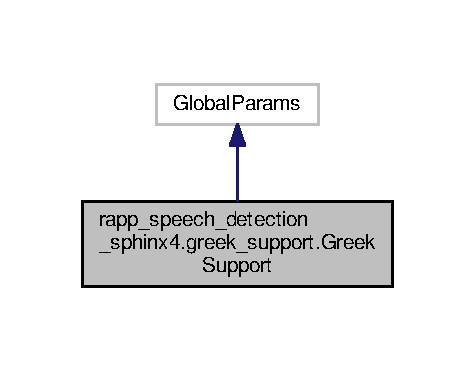
\includegraphics[width=260pt]{classrapp__speech__detection__sphinx4_1_1greek__support_1_1GreekSupport__inherit__graph}
\end{center}
\end{figure}


Collaboration diagram for rapp\-\_\-speech\-\_\-detection\-\_\-sphinx4.\-greek\-\_\-support.\-Greek\-Support\-:
\nopagebreak
\begin{figure}[H]
\begin{center}
\leavevmode
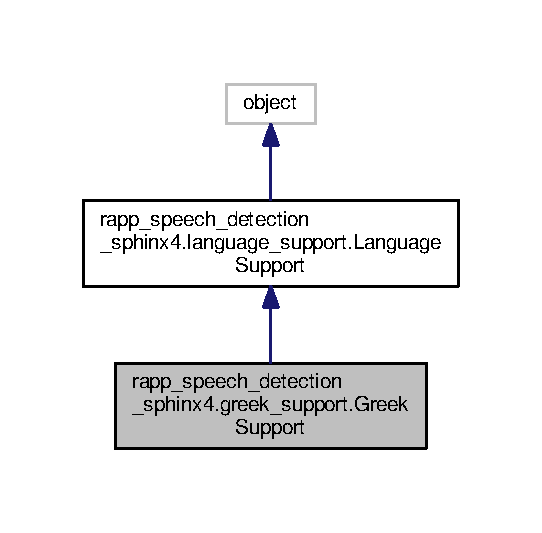
\includegraphics[width=260pt]{classrapp__speech__detection__sphinx4_1_1greek__support_1_1GreekSupport__coll__graph}
\end{center}
\end{figure}
\subsection*{Public Member Functions}
\begin{DoxyCompactItemize}
\item 
def \hyperlink{classrapp__speech__detection__sphinx4_1_1greek__support_1_1GreekSupport_a11ade953742b11f592db3fdee75d97c1}{\-\_\-\-\_\-init\-\_\-\-\_\-}
\begin{DoxyCompactList}\small\item\em Performs initializations. \end{DoxyCompactList}\item 
def \hyperlink{classrapp__speech__detection__sphinx4_1_1greek__support_1_1GreekSupport_aaf3225dba3273dbd5fd7b01944e20289}{get\-Limited\-Vocebulary\-Configuration}
\begin{DoxyCompactList}\small\item\em Computes the Limited Greek Configuration. \end{DoxyCompactList}\end{DoxyCompactItemize}
\subsection*{Private Member Functions}
\begin{DoxyCompactItemize}
\item 
def \hyperlink{classrapp__speech__detection__sphinx4_1_1greek__support_1_1GreekSupport_ac5823a37a949ba4bf9669906913e064b}{\-\_\-configure\-Letters}
\begin{DoxyCompactList}\small\item\em Creates the basic Greek letter to English configuration. \end{DoxyCompactList}\item 
def \hyperlink{classrapp__speech__detection__sphinx4_1_1greek__support_1_1GreekSupport_a26445e371062313c7e1a7a04562a3bf7}{\-\_\-englify\-\_\-words}
\begin{DoxyCompactList}\small\item\em Englify Greek words. \end{DoxyCompactList}\item 
def \hyperlink{classrapp__speech__detection__sphinx4_1_1greek__support_1_1GreekSupport_ac7e3b9ebc81d7c52b0892edf79ae5edc}{\-\_\-transform\-Words}
\begin{DoxyCompactList}\small\item\em Transforms the Greek words into phonemes for the Sphinx configuration. \end{DoxyCompactList}\end{DoxyCompactItemize}
\subsection*{Private Attributes}
\begin{DoxyCompactItemize}
\item 
\hyperlink{classrapp__speech__detection__sphinx4_1_1greek__support_1_1GreekSupport_a533b86fa7f9105c49d0a729140d76c27}{\-\_\-all\-\_\-special\-\_\-two\-\_\-digit\-\_\-letters}
\begin{DoxyCompactList}\small\item\em All special two digit Greek letter-\/$>$English phonemes mapping. \end{DoxyCompactList}\item 
\hyperlink{classrapp__speech__detection__sphinx4_1_1greek__support_1_1GreekSupport_a69f45d4217814cba24edcb2e5597956b}{\-\_\-capital\-\_\-letters}
\begin{DoxyCompactList}\small\item\em Greek uppercase to lowercase mapping. \end{DoxyCompactList}\item 
\hyperlink{classrapp__speech__detection__sphinx4_1_1greek__support_1_1GreekSupport_aff5fd96d6423b28163b900c2ea06e188}{\-\_\-english\-\_\-support}
\begin{DoxyCompactList}\small\item\em Allows the creation of configuration files for English words. \end{DoxyCompactList}\item 
\hyperlink{classrapp__speech__detection__sphinx4_1_1greek__support_1_1GreekSupport_a6115cc5d04ce7f8e891f5b112f8d4151}{\-\_\-letters}
\begin{DoxyCompactList}\small\item\em Standard Greek letter-\/$>$English phonemes mapping. \end{DoxyCompactList}\item 
\hyperlink{classrapp__speech__detection__sphinx4_1_1greek__support_1_1GreekSupport_a553a5e8b07dc6b3b9b83a2f814535204}{\-\_\-literal\-\_\-letters}
\begin{DoxyCompactList}\small\item\em Greek letters-\/$>$English letters mapping. \end{DoxyCompactList}\item 
\hyperlink{classrapp__speech__detection__sphinx4_1_1greek__support_1_1GreekSupport_ac660aeb52c669c9e0bd81d9cac50c3d6}{\-\_\-phonemes}
\begin{DoxyCompactList}\small\item\em Greek words-\/$>$English standard phonemes mapping. \end{DoxyCompactList}\item 
\hyperlink{classrapp__speech__detection__sphinx4_1_1greek__support_1_1GreekSupport_acdc908eced1c5243b5f8cb75dae0cd8b}{\-\_\-s\-\_\-specific\-\_\-rules}
\begin{DoxyCompactList}\small\item\em Special Greek words -\/$>$English phonemes mapping. \end{DoxyCompactList}\item 
\hyperlink{classrapp__speech__detection__sphinx4_1_1greek__support_1_1GreekSupport_a556cca34cd5c3e51561b77a4ebcf7510}{\-\_\-special\-\_\-two\-\_\-digit\-\_\-letters}
\begin{DoxyCompactList}\small\item\em Special two digit Greek letter-\/$>$English phonemes mapping. \end{DoxyCompactList}\item 
\hyperlink{classrapp__speech__detection__sphinx4_1_1greek__support_1_1GreekSupport_a86a67ca628328d247fd54cefe02c4962}{\-\_\-two\-\_\-digit\-\_\-letters}
\begin{DoxyCompactList}\small\item\em Two digit Greek letters-\/$>$English phonemes mapping. \end{DoxyCompactList}\end{DoxyCompactItemize}


\subsection{Detailed Description}
Allows the creation of configuration files for Greek Sphinx speech recognition. 

Also supports multilanguage words (English/\-Greek) by utilizing \hyperlink{classrapp__speech__detection__sphinx4_1_1english__support_1_1EnglishSupport}{english\-\_\-support.\-English\-Support} 

Definition at line 30 of file greek\-\_\-support.\-py.



\subsection{Constructor \& Destructor Documentation}
\hypertarget{classrapp__speech__detection__sphinx4_1_1greek__support_1_1GreekSupport_a11ade953742b11f592db3fdee75d97c1}{\index{rapp\-\_\-speech\-\_\-detection\-\_\-sphinx4\-::greek\-\_\-support\-::\-Greek\-Support@{rapp\-\_\-speech\-\_\-detection\-\_\-sphinx4\-::greek\-\_\-support\-::\-Greek\-Support}!\-\_\-\-\_\-init\-\_\-\-\_\-@{\-\_\-\-\_\-init\-\_\-\-\_\-}}
\index{\-\_\-\-\_\-init\-\_\-\-\_\-@{\-\_\-\-\_\-init\-\_\-\-\_\-}!rapp_speech_detection_sphinx4::greek_support::GreekSupport@{rapp\-\_\-speech\-\_\-detection\-\_\-sphinx4\-::greek\-\_\-support\-::\-Greek\-Support}}
\subsubsection[{\-\_\-\-\_\-init\-\_\-\-\_\-}]{\setlength{\rightskip}{0pt plus 5cm}def rapp\-\_\-speech\-\_\-detection\-\_\-sphinx4.\-greek\-\_\-support.\-Greek\-Support.\-\_\-\-\_\-init\-\_\-\-\_\- (
\begin{DoxyParamCaption}
\item[{}]{self}
\end{DoxyParamCaption}
)}}\label{classrapp__speech__detection__sphinx4_1_1greek__support_1_1GreekSupport_a11ade953742b11f592db3fdee75d97c1}


Performs initializations. 



Definition at line 33 of file greek\-\_\-support.\-py.



\subsection{Member Function Documentation}
\hypertarget{classrapp__speech__detection__sphinx4_1_1greek__support_1_1GreekSupport_ac5823a37a949ba4bf9669906913e064b}{\index{rapp\-\_\-speech\-\_\-detection\-\_\-sphinx4\-::greek\-\_\-support\-::\-Greek\-Support@{rapp\-\_\-speech\-\_\-detection\-\_\-sphinx4\-::greek\-\_\-support\-::\-Greek\-Support}!\-\_\-configure\-Letters@{\-\_\-configure\-Letters}}
\index{\-\_\-configure\-Letters@{\-\_\-configure\-Letters}!rapp_speech_detection_sphinx4::greek_support::GreekSupport@{rapp\-\_\-speech\-\_\-detection\-\_\-sphinx4\-::greek\-\_\-support\-::\-Greek\-Support}}
\subsubsection[{\-\_\-configure\-Letters}]{\setlength{\rightskip}{0pt plus 5cm}def rapp\-\_\-speech\-\_\-detection\-\_\-sphinx4.\-greek\-\_\-support.\-Greek\-Support.\-\_\-configure\-Letters (
\begin{DoxyParamCaption}
\item[{}]{self}
\end{DoxyParamCaption}
)\hspace{0.3cm}{\ttfamily [private]}}}\label{classrapp__speech__detection__sphinx4_1_1greek__support_1_1GreekSupport_ac5823a37a949ba4bf9669906913e064b}


Creates the basic Greek letter to English configuration. 



Definition at line 69 of file greek\-\_\-support.\-py.

\hypertarget{classrapp__speech__detection__sphinx4_1_1greek__support_1_1GreekSupport_a26445e371062313c7e1a7a04562a3bf7}{\index{rapp\-\_\-speech\-\_\-detection\-\_\-sphinx4\-::greek\-\_\-support\-::\-Greek\-Support@{rapp\-\_\-speech\-\_\-detection\-\_\-sphinx4\-::greek\-\_\-support\-::\-Greek\-Support}!\-\_\-englify\-\_\-words@{\-\_\-englify\-\_\-words}}
\index{\-\_\-englify\-\_\-words@{\-\_\-englify\-\_\-words}!rapp_speech_detection_sphinx4::greek_support::GreekSupport@{rapp\-\_\-speech\-\_\-detection\-\_\-sphinx4\-::greek\-\_\-support\-::\-Greek\-Support}}
\subsubsection[{\-\_\-englify\-\_\-words}]{\setlength{\rightskip}{0pt plus 5cm}def rapp\-\_\-speech\-\_\-detection\-\_\-sphinx4.\-greek\-\_\-support.\-Greek\-Support.\-\_\-englify\-\_\-words (
\begin{DoxyParamCaption}
\item[{}]{self, }
\item[{}]{words}
\end{DoxyParamCaption}
)\hspace{0.3cm}{\ttfamily [private]}}}\label{classrapp__speech__detection__sphinx4_1_1greek__support_1_1GreekSupport_a26445e371062313c7e1a7a04562a3bf7}


Englify Greek words. 


\begin{DoxyParams}{Parameters}
{\em words} & \mbox{[}list\-::string\mbox{]} The set of Greek words \\
\hline
\end{DoxyParams}


Definition at line 308 of file greek\-\_\-support.\-py.

\hypertarget{classrapp__speech__detection__sphinx4_1_1greek__support_1_1GreekSupport_ac7e3b9ebc81d7c52b0892edf79ae5edc}{\index{rapp\-\_\-speech\-\_\-detection\-\_\-sphinx4\-::greek\-\_\-support\-::\-Greek\-Support@{rapp\-\_\-speech\-\_\-detection\-\_\-sphinx4\-::greek\-\_\-support\-::\-Greek\-Support}!\-\_\-transform\-Words@{\-\_\-transform\-Words}}
\index{\-\_\-transform\-Words@{\-\_\-transform\-Words}!rapp_speech_detection_sphinx4::greek_support::GreekSupport@{rapp\-\_\-speech\-\_\-detection\-\_\-sphinx4\-::greek\-\_\-support\-::\-Greek\-Support}}
\subsubsection[{\-\_\-transform\-Words}]{\setlength{\rightskip}{0pt plus 5cm}def rapp\-\_\-speech\-\_\-detection\-\_\-sphinx4.\-greek\-\_\-support.\-Greek\-Support.\-\_\-transform\-Words (
\begin{DoxyParamCaption}
\item[{}]{self, }
\item[{}]{words}
\end{DoxyParamCaption}
)\hspace{0.3cm}{\ttfamily [private]}}}\label{classrapp__speech__detection__sphinx4_1_1greek__support_1_1GreekSupport_ac7e3b9ebc81d7c52b0892edf79ae5edc}


Transforms the Greek words into phonemes for the Sphinx configuration. 


\begin{DoxyParams}{Parameters}
{\em words} & \mbox{[}list\-::string\mbox{]} The set of Greek words\\
\hline
\end{DoxyParams}
\begin{DoxyReturn}{Returns}
enhanced\-\_\-words \mbox{[}dictionary\mbox{]} The Greek word-\/$>$phonemes mapping 

englified\-\_\-words \mbox{[}dictionary\mbox{]} The Greek word-\/$>$Englified Greek word mapping 
\end{DoxyReturn}


Definition at line 259 of file greek\-\_\-support.\-py.

\hypertarget{classrapp__speech__detection__sphinx4_1_1greek__support_1_1GreekSupport_aaf3225dba3273dbd5fd7b01944e20289}{\index{rapp\-\_\-speech\-\_\-detection\-\_\-sphinx4\-::greek\-\_\-support\-::\-Greek\-Support@{rapp\-\_\-speech\-\_\-detection\-\_\-sphinx4\-::greek\-\_\-support\-::\-Greek\-Support}!get\-Limited\-Vocebulary\-Configuration@{get\-Limited\-Vocebulary\-Configuration}}
\index{get\-Limited\-Vocebulary\-Configuration@{get\-Limited\-Vocebulary\-Configuration}!rapp_speech_detection_sphinx4::greek_support::GreekSupport@{rapp\-\_\-speech\-\_\-detection\-\_\-sphinx4\-::greek\-\_\-support\-::\-Greek\-Support}}
\subsubsection[{get\-Limited\-Vocebulary\-Configuration}]{\setlength{\rightskip}{0pt plus 5cm}def rapp\-\_\-speech\-\_\-detection\-\_\-sphinx4.\-greek\-\_\-support.\-Greek\-Support.\-get\-Limited\-Vocebulary\-Configuration (
\begin{DoxyParamCaption}
\item[{}]{self, }
\item[{}]{words, }
\item[{}]{grammar, }
\item[{}]{sentences}
\end{DoxyParamCaption}
)}}\label{classrapp__speech__detection__sphinx4_1_1greek__support_1_1GreekSupport_aaf3225dba3273dbd5fd7b01944e20289}


Computes the Limited Greek Configuration. 


\begin{DoxyParams}{Parameters}
{\em words} & \mbox{[}list\-::string\mbox{]} The set of words to be identified \\
\hline
{\em grammar} & \mbox{[}list\-::string\mbox{]} The Sphinx grammar parameter \\
\hline
{\em sentences} & \mbox{[}list\-::string\mbox{]} The Sphinx sentences parameter\\
\hline
\end{DoxyParams}
\begin{DoxyReturn}{Returns}
limited\-\_\-sphinx\-\_\-configuration \mbox{[}dictionary\mbox{]} The Limited Greek configuration 

englified\-\_\-to\-\_\-greek\-\_\-dict \mbox{[}dictionary\mbox{]} A dictionary to transform the englified greek words to actual greek words 
\end{DoxyReturn}


Definition at line 329 of file greek\-\_\-support.\-py.



\subsection{Member Data Documentation}
\hypertarget{classrapp__speech__detection__sphinx4_1_1greek__support_1_1GreekSupport_a533b86fa7f9105c49d0a729140d76c27}{\index{rapp\-\_\-speech\-\_\-detection\-\_\-sphinx4\-::greek\-\_\-support\-::\-Greek\-Support@{rapp\-\_\-speech\-\_\-detection\-\_\-sphinx4\-::greek\-\_\-support\-::\-Greek\-Support}!\-\_\-all\-\_\-special\-\_\-two\-\_\-digit\-\_\-letters@{\-\_\-all\-\_\-special\-\_\-two\-\_\-digit\-\_\-letters}}
\index{\-\_\-all\-\_\-special\-\_\-two\-\_\-digit\-\_\-letters@{\-\_\-all\-\_\-special\-\_\-two\-\_\-digit\-\_\-letters}!rapp_speech_detection_sphinx4::greek_support::GreekSupport@{rapp\-\_\-speech\-\_\-detection\-\_\-sphinx4\-::greek\-\_\-support\-::\-Greek\-Support}}
\subsubsection[{\-\_\-all\-\_\-special\-\_\-two\-\_\-digit\-\_\-letters}]{\setlength{\rightskip}{0pt plus 5cm}rapp\-\_\-speech\-\_\-detection\-\_\-sphinx4.\-greek\-\_\-support.\-Greek\-Support.\-\_\-all\-\_\-special\-\_\-two\-\_\-digit\-\_\-letters\hspace{0.3cm}{\ttfamily [private]}}}\label{classrapp__speech__detection__sphinx4_1_1greek__support_1_1GreekSupport_a533b86fa7f9105c49d0a729140d76c27}


All special two digit Greek letter-\/$>$English phonemes mapping. 



Definition at line 58 of file greek\-\_\-support.\-py.

\hypertarget{classrapp__speech__detection__sphinx4_1_1greek__support_1_1GreekSupport_a69f45d4217814cba24edcb2e5597956b}{\index{rapp\-\_\-speech\-\_\-detection\-\_\-sphinx4\-::greek\-\_\-support\-::\-Greek\-Support@{rapp\-\_\-speech\-\_\-detection\-\_\-sphinx4\-::greek\-\_\-support\-::\-Greek\-Support}!\-\_\-capital\-\_\-letters@{\-\_\-capital\-\_\-letters}}
\index{\-\_\-capital\-\_\-letters@{\-\_\-capital\-\_\-letters}!rapp_speech_detection_sphinx4::greek_support::GreekSupport@{rapp\-\_\-speech\-\_\-detection\-\_\-sphinx4\-::greek\-\_\-support\-::\-Greek\-Support}}
\subsubsection[{\-\_\-capital\-\_\-letters}]{\setlength{\rightskip}{0pt plus 5cm}rapp\-\_\-speech\-\_\-detection\-\_\-sphinx4.\-greek\-\_\-support.\-Greek\-Support.\-\_\-capital\-\_\-letters\hspace{0.3cm}{\ttfamily [private]}}}\label{classrapp__speech__detection__sphinx4_1_1greek__support_1_1GreekSupport_a69f45d4217814cba24edcb2e5597956b}


Greek uppercase to lowercase mapping. 



Definition at line 50 of file greek\-\_\-support.\-py.

\hypertarget{classrapp__speech__detection__sphinx4_1_1greek__support_1_1GreekSupport_aff5fd96d6423b28163b900c2ea06e188}{\index{rapp\-\_\-speech\-\_\-detection\-\_\-sphinx4\-::greek\-\_\-support\-::\-Greek\-Support@{rapp\-\_\-speech\-\_\-detection\-\_\-sphinx4\-::greek\-\_\-support\-::\-Greek\-Support}!\-\_\-english\-\_\-support@{\-\_\-english\-\_\-support}}
\index{\-\_\-english\-\_\-support@{\-\_\-english\-\_\-support}!rapp_speech_detection_sphinx4::greek_support::GreekSupport@{rapp\-\_\-speech\-\_\-detection\-\_\-sphinx4\-::greek\-\_\-support\-::\-Greek\-Support}}
\subsubsection[{\-\_\-english\-\_\-support}]{\setlength{\rightskip}{0pt plus 5cm}rapp\-\_\-speech\-\_\-detection\-\_\-sphinx4.\-greek\-\_\-support.\-Greek\-Support.\-\_\-english\-\_\-support\hspace{0.3cm}{\ttfamily [private]}}}\label{classrapp__speech__detection__sphinx4_1_1greek__support_1_1GreekSupport_aff5fd96d6423b28163b900c2ea06e188}


Allows the creation of configuration files for English words. 

Instantiates \hyperlink{classrapp__speech__detection__sphinx4_1_1english__support_1_1EnglishSupport}{english\-\_\-support.\-English\-Support} to identify english words 

Definition at line 47 of file greek\-\_\-support.\-py.

\hypertarget{classrapp__speech__detection__sphinx4_1_1greek__support_1_1GreekSupport_a6115cc5d04ce7f8e891f5b112f8d4151}{\index{rapp\-\_\-speech\-\_\-detection\-\_\-sphinx4\-::greek\-\_\-support\-::\-Greek\-Support@{rapp\-\_\-speech\-\_\-detection\-\_\-sphinx4\-::greek\-\_\-support\-::\-Greek\-Support}!\-\_\-letters@{\-\_\-letters}}
\index{\-\_\-letters@{\-\_\-letters}!rapp_speech_detection_sphinx4::greek_support::GreekSupport@{rapp\-\_\-speech\-\_\-detection\-\_\-sphinx4\-::greek\-\_\-support\-::\-Greek\-Support}}
\subsubsection[{\-\_\-letters}]{\setlength{\rightskip}{0pt plus 5cm}rapp\-\_\-speech\-\_\-detection\-\_\-sphinx4.\-greek\-\_\-support.\-Greek\-Support.\-\_\-letters\hspace{0.3cm}{\ttfamily [private]}}}\label{classrapp__speech__detection__sphinx4_1_1greek__support_1_1GreekSupport_a6115cc5d04ce7f8e891f5b112f8d4151}


Standard Greek letter-\/$>$English phonemes mapping. 



Definition at line 62 of file greek\-\_\-support.\-py.

\hypertarget{classrapp__speech__detection__sphinx4_1_1greek__support_1_1GreekSupport_a553a5e8b07dc6b3b9b83a2f814535204}{\index{rapp\-\_\-speech\-\_\-detection\-\_\-sphinx4\-::greek\-\_\-support\-::\-Greek\-Support@{rapp\-\_\-speech\-\_\-detection\-\_\-sphinx4\-::greek\-\_\-support\-::\-Greek\-Support}!\-\_\-literal\-\_\-letters@{\-\_\-literal\-\_\-letters}}
\index{\-\_\-literal\-\_\-letters@{\-\_\-literal\-\_\-letters}!rapp_speech_detection_sphinx4::greek_support::GreekSupport@{rapp\-\_\-speech\-\_\-detection\-\_\-sphinx4\-::greek\-\_\-support\-::\-Greek\-Support}}
\subsubsection[{\-\_\-literal\-\_\-letters}]{\setlength{\rightskip}{0pt plus 5cm}rapp\-\_\-speech\-\_\-detection\-\_\-sphinx4.\-greek\-\_\-support.\-Greek\-Support.\-\_\-literal\-\_\-letters\hspace{0.3cm}{\ttfamily [private]}}}\label{classrapp__speech__detection__sphinx4_1_1greek__support_1_1GreekSupport_a553a5e8b07dc6b3b9b83a2f814535204}


Greek letters-\/$>$English letters mapping. 



Definition at line 64 of file greek\-\_\-support.\-py.

\hypertarget{classrapp__speech__detection__sphinx4_1_1greek__support_1_1GreekSupport_ac660aeb52c669c9e0bd81d9cac50c3d6}{\index{rapp\-\_\-speech\-\_\-detection\-\_\-sphinx4\-::greek\-\_\-support\-::\-Greek\-Support@{rapp\-\_\-speech\-\_\-detection\-\_\-sphinx4\-::greek\-\_\-support\-::\-Greek\-Support}!\-\_\-phonemes@{\-\_\-phonemes}}
\index{\-\_\-phonemes@{\-\_\-phonemes}!rapp_speech_detection_sphinx4::greek_support::GreekSupport@{rapp\-\_\-speech\-\_\-detection\-\_\-sphinx4\-::greek\-\_\-support\-::\-Greek\-Support}}
\subsubsection[{\-\_\-phonemes}]{\setlength{\rightskip}{0pt plus 5cm}rapp\-\_\-speech\-\_\-detection\-\_\-sphinx4.\-greek\-\_\-support.\-Greek\-Support.\-\_\-phonemes\hspace{0.3cm}{\ttfamily [private]}}}\label{classrapp__speech__detection__sphinx4_1_1greek__support_1_1GreekSupport_ac660aeb52c669c9e0bd81d9cac50c3d6}


Greek words-\/$>$English standard phonemes mapping. 



Definition at line 52 of file greek\-\_\-support.\-py.

\hypertarget{classrapp__speech__detection__sphinx4_1_1greek__support_1_1GreekSupport_acdc908eced1c5243b5f8cb75dae0cd8b}{\index{rapp\-\_\-speech\-\_\-detection\-\_\-sphinx4\-::greek\-\_\-support\-::\-Greek\-Support@{rapp\-\_\-speech\-\_\-detection\-\_\-sphinx4\-::greek\-\_\-support\-::\-Greek\-Support}!\-\_\-s\-\_\-specific\-\_\-rules@{\-\_\-s\-\_\-specific\-\_\-rules}}
\index{\-\_\-s\-\_\-specific\-\_\-rules@{\-\_\-s\-\_\-specific\-\_\-rules}!rapp_speech_detection_sphinx4::greek_support::GreekSupport@{rapp\-\_\-speech\-\_\-detection\-\_\-sphinx4\-::greek\-\_\-support\-::\-Greek\-Support}}
\subsubsection[{\-\_\-s\-\_\-specific\-\_\-rules}]{\setlength{\rightskip}{0pt plus 5cm}rapp\-\_\-speech\-\_\-detection\-\_\-sphinx4.\-greek\-\_\-support.\-Greek\-Support.\-\_\-s\-\_\-specific\-\_\-rules\hspace{0.3cm}{\ttfamily [private]}}}\label{classrapp__speech__detection__sphinx4_1_1greek__support_1_1GreekSupport_acdc908eced1c5243b5f8cb75dae0cd8b}


Special Greek words -\/$>$English phonemes mapping. 



Definition at line 60 of file greek\-\_\-support.\-py.

\hypertarget{classrapp__speech__detection__sphinx4_1_1greek__support_1_1GreekSupport_a556cca34cd5c3e51561b77a4ebcf7510}{\index{rapp\-\_\-speech\-\_\-detection\-\_\-sphinx4\-::greek\-\_\-support\-::\-Greek\-Support@{rapp\-\_\-speech\-\_\-detection\-\_\-sphinx4\-::greek\-\_\-support\-::\-Greek\-Support}!\-\_\-special\-\_\-two\-\_\-digit\-\_\-letters@{\-\_\-special\-\_\-two\-\_\-digit\-\_\-letters}}
\index{\-\_\-special\-\_\-two\-\_\-digit\-\_\-letters@{\-\_\-special\-\_\-two\-\_\-digit\-\_\-letters}!rapp_speech_detection_sphinx4::greek_support::GreekSupport@{rapp\-\_\-speech\-\_\-detection\-\_\-sphinx4\-::greek\-\_\-support\-::\-Greek\-Support}}
\subsubsection[{\-\_\-special\-\_\-two\-\_\-digit\-\_\-letters}]{\setlength{\rightskip}{0pt plus 5cm}rapp\-\_\-speech\-\_\-detection\-\_\-sphinx4.\-greek\-\_\-support.\-Greek\-Support.\-\_\-special\-\_\-two\-\_\-digit\-\_\-letters\hspace{0.3cm}{\ttfamily [private]}}}\label{classrapp__speech__detection__sphinx4_1_1greek__support_1_1GreekSupport_a556cca34cd5c3e51561b77a4ebcf7510}


Special two digit Greek letter-\/$>$English phonemes mapping. 



Definition at line 56 of file greek\-\_\-support.\-py.

\hypertarget{classrapp__speech__detection__sphinx4_1_1greek__support_1_1GreekSupport_a86a67ca628328d247fd54cefe02c4962}{\index{rapp\-\_\-speech\-\_\-detection\-\_\-sphinx4\-::greek\-\_\-support\-::\-Greek\-Support@{rapp\-\_\-speech\-\_\-detection\-\_\-sphinx4\-::greek\-\_\-support\-::\-Greek\-Support}!\-\_\-two\-\_\-digit\-\_\-letters@{\-\_\-two\-\_\-digit\-\_\-letters}}
\index{\-\_\-two\-\_\-digit\-\_\-letters@{\-\_\-two\-\_\-digit\-\_\-letters}!rapp_speech_detection_sphinx4::greek_support::GreekSupport@{rapp\-\_\-speech\-\_\-detection\-\_\-sphinx4\-::greek\-\_\-support\-::\-Greek\-Support}}
\subsubsection[{\-\_\-two\-\_\-digit\-\_\-letters}]{\setlength{\rightskip}{0pt plus 5cm}rapp\-\_\-speech\-\_\-detection\-\_\-sphinx4.\-greek\-\_\-support.\-Greek\-Support.\-\_\-two\-\_\-digit\-\_\-letters\hspace{0.3cm}{\ttfamily [private]}}}\label{classrapp__speech__detection__sphinx4_1_1greek__support_1_1GreekSupport_a86a67ca628328d247fd54cefe02c4962}


Two digit Greek letters-\/$>$English phonemes mapping. 



Definition at line 54 of file greek\-\_\-support.\-py.



The documentation for this class was generated from the following file\-:\begin{DoxyCompactItemize}
\item 
/home/travis/rapp\-\_\-temp/rapp-\/platform/rapp\-\_\-speech\-\_\-detection\-\_\-sphinx4/src/rapp\-\_\-speech\-\_\-detection\-\_\-sphinx4/\hyperlink{greek__support_8py}{greek\-\_\-support.\-py}\end{DoxyCompactItemize}

\hypertarget{classKnowrobWrapper}{\section{Knowrob\-Wrapper Class Reference}
\label{classKnowrobWrapper}\index{Knowrob\-Wrapper@{Knowrob\-Wrapper}}
}


Class \hyperlink{classKnowrobWrapperCommunications}{Knowrob\-Wrapper\-Communications} contains all the necessary knowrob wrapper functions.  




{\ttfamily \#include $<$knowrob\-\_\-wrapper.\-h$>$}

\subsection*{Public Member Functions}
\begin{DoxyCompactItemize}
\item 
\hyperlink{classKnowrobWrapper_adfaff3e5574aa56d54fcf31c36fd3450}{Knowrob\-Wrapper} (ros\-::\-Node\-Handle nh)
\begin{DoxyCompactList}\small\item\em Default constructor. \end{DoxyCompactList}\item 
rapp\-\_\-platform\-\_\-ros\-\_\-communications\-::assert\-Retract\-Attribute\-Srv\-::\-Response \hyperlink{classKnowrobWrapper_a7dc0ea0f609179e541e51b5351c47243}{assert\-Attribute\-Value} (rapp\-\_\-platform\-\_\-ros\-\_\-communications\-::assert\-Retract\-Attribute\-Srv\-::\-Request req)
\begin{DoxyCompactList}\small\item\em Implements the assert\-Retract\-Attribute R\-O\-S service. \end{DoxyCompactList}\item 
rapp\-\_\-platform\-\_\-ros\-\_\-communications\-::clear\-User\-Performance\-Cognitve\-Tests\-Srv\-::\-Response \hyperlink{classKnowrobWrapper_ad80bcfe67c92da6bd3d5edf22d465c38}{clear\-\_\-user\-\_\-cognitive\-\_\-tests\-\_\-performance\-\_\-records} (rapp\-\_\-platform\-\_\-ros\-\_\-communications\-::clear\-User\-Performance\-Cognitve\-Tests\-Srv\-::\-Request req)
\begin{DoxyCompactList}\small\item\em Implements the clear\-\_\-user\-\_\-cognitive\-\_\-tests\-\_\-performance\-\_\-records R\-O\-S service. \end{DoxyCompactList}\item 
rapp\-\_\-platform\-\_\-ros\-\_\-communications\-::cognitive\-Tests\-Of\-Type\-Srv\-::\-Response \hyperlink{classKnowrobWrapper_a6b97ec7ecde086f444cfce881c4625dc}{cognitive\-\_\-tests\-\_\-of\-\_\-type} (rapp\-\_\-platform\-\_\-ros\-\_\-communications\-::cognitive\-Tests\-Of\-Type\-Srv\-::\-Request req)
\begin{DoxyCompactList}\small\item\em Implements the cognitive\-\_\-tests\-\_\-of\-\_\-type R\-O\-S service. \end{DoxyCompactList}\item 
rapp\-\_\-platform\-\_\-ros\-\_\-communications\-::create\-Cognitive\-Exercise\-Test\-Srv\-::\-Response \hyperlink{classKnowrobWrapper_a21bb40079cf4cd21afe114f51ec6125b}{create\-\_\-cognitve\-\_\-tests} (rapp\-\_\-platform\-\_\-ros\-\_\-communications\-::create\-Cognitive\-Exercise\-Test\-Srv\-::\-Request req)
\begin{DoxyCompactList}\small\item\em Implements the create\-\_\-cognitve\-\_\-tests R\-O\-S service. \end{DoxyCompactList}\item 
rapp\-\_\-platform\-\_\-ros\-\_\-communications\-::create\-Ontology\-Alias\-Srv\-::\-Response \hyperlink{classKnowrobWrapper_a6b5c92e16d3592a63d6509dbca1317fe}{create\-\_\-ontology\-\_\-alias} (rapp\-\_\-platform\-\_\-ros\-\_\-communications\-::create\-Ontology\-Alias\-Srv\-::\-Request req)
\begin{DoxyCompactList}\small\item\em Implements the create\-\_\-ontology\-\_\-alias R\-O\-S service. \end{DoxyCompactList}\item 
std\-::string \hyperlink{classKnowrobWrapper_a85be3123e645ca77004c7461e097a15e}{create\-\_\-ontology\-\_\-alias\-\_\-for\-\_\-new\-\_\-user} (std\-::string user\-\_\-id)
\begin{DoxyCompactList}\small\item\em Creates a new ontology alias for a user. \end{DoxyCompactList}\item 
rapp\-\_\-platform\-\_\-ros\-\_\-communications\-::create\-Instance\-Srv\-::\-Response \hyperlink{classKnowrobWrapper_a798a52556983073055944fd1c51495de}{create\-Instance\-Query} (rapp\-\_\-platform\-\_\-ros\-\_\-communications\-::create\-Instance\-Srv\-::\-Request req)
\begin{DoxyCompactList}\small\item\em Implements the create\-Instance R\-O\-S service. \end{DoxyCompactList}\item 
rapp\-\_\-platform\-\_\-ros\-\_\-communications\-::ontology\-Load\-Dump\-Srv\-::\-Response \hyperlink{classKnowrobWrapper_a86796d95e57f4620474dab7e1f2df128}{dump\-Ontology\-Query} (rapp\-\_\-platform\-\_\-ros\-\_\-communications\-::ontology\-Load\-Dump\-Srv\-::\-Request req)
\begin{DoxyCompactList}\small\item\em Implements the dump\-Ontology R\-O\-S service. \end{DoxyCompactList}\item 
std\-::string \hyperlink{classKnowrobWrapper_af50b1b512559d86a74c6de69a34ac3cc}{get\-\_\-ontology\-\_\-alias} (std\-::string user\-\_\-id)
\begin{DoxyCompactList}\small\item\em Returns the ontology alias of the user. \end{DoxyCompactList}\item 
rapp\-\_\-platform\-\_\-ros\-\_\-communications\-::ontology\-Is\-Sub\-Super\-Class\-Of\-Srv\-::\-Response \hyperlink{classKnowrobWrapper_a0608e1b44bdbf4925b8f3df7433e1b4d}{is\-Sub\-Superclass\-Of\-Query} (rapp\-\_\-platform\-\_\-ros\-\_\-communications\-::ontology\-Is\-Sub\-Super\-Class\-Of\-Srv\-::\-Request req)
\begin{DoxyCompactList}\small\item\em Implements the is\-Sub\-Superclass R\-O\-S service. \end{DoxyCompactList}\item 
rapp\-\_\-platform\-\_\-ros\-\_\-communications\-::ontology\-Load\-Dump\-Srv\-::\-Response \hyperlink{classKnowrobWrapper_acb503520ab8db0e11b5d6511c7d1a69b}{load\-Ontology\-Query} (rapp\-\_\-platform\-\_\-ros\-\_\-communications\-::ontology\-Load\-Dump\-Srv\-::\-Request req)
\begin{DoxyCompactList}\small\item\em Implements the load\-Ontology R\-O\-S service. \end{DoxyCompactList}\item 
rapp\-\_\-platform\-\_\-ros\-\_\-communications\-::record\-User\-Performance\-Cognitive\-Tests\-Srv\-::\-Response \hyperlink{classKnowrobWrapper_a77d7c7d52db582093065271ebb6d8be7}{record\-\_\-user\-\_\-cognitive\-\_\-tests\-\_\-performance} (rapp\-\_\-platform\-\_\-ros\-\_\-communications\-::record\-User\-Performance\-Cognitive\-Tests\-Srv\-::\-Request req)
\begin{DoxyCompactList}\small\item\em Implements the record\-\_\-user\-\_\-cognitive\-\_\-tests\-\_\-performance R\-O\-S service. \end{DoxyCompactList}\item 
rapp\-\_\-platform\-\_\-ros\-\_\-communications\-::ontology\-Sub\-Super\-Classes\-Of\-Srv\-::\-Response \hyperlink{classKnowrobWrapper_a6e2ee6a631a705466a490f37ecf8afd5}{subclasses\-Of\-Query} (rapp\-\_\-platform\-\_\-ros\-\_\-communications\-::ontology\-Sub\-Super\-Classes\-Of\-Srv\-::\-Request req)
\begin{DoxyCompactList}\small\item\em Implements the subclasses\-Of R\-O\-S service. \end{DoxyCompactList}\item 
rapp\-\_\-platform\-\_\-ros\-\_\-communications\-::ontology\-Sub\-Super\-Classes\-Of\-Srv\-::\-Response \hyperlink{classKnowrobWrapper_a5347e77b2c2bf866c91b883f7eb19e42}{superclasses\-Of\-Query} (rapp\-\_\-platform\-\_\-ros\-\_\-communications\-::ontology\-Sub\-Super\-Classes\-Of\-Srv\-::\-Request req)
\begin{DoxyCompactList}\small\item\em Implements the superclasses\-Of R\-O\-S service. \end{DoxyCompactList}\item 
rapp\-\_\-platform\-\_\-ros\-\_\-communications\-::return\-User\-Instances\-Of\-Class\-Srv\-::\-Response \hyperlink{classKnowrobWrapper_a458f965a337460f5822c71bab7a9180d}{user\-\_\-instances\-\_\-of\-\_\-class} (rapp\-\_\-platform\-\_\-ros\-\_\-communications\-::return\-User\-Instances\-Of\-Class\-Srv\-::\-Request req)
\begin{DoxyCompactList}\small\item\em Implements the return\-User\-Instances\-Of\-Class R\-O\-S service. \end{DoxyCompactList}\item 
rapp\-\_\-platform\-\_\-ros\-\_\-communications\-::user\-Performance\-Cognitve\-Tests\-Srv\-::\-Response \hyperlink{classKnowrobWrapper_aada77adb91efe2be3ddd2ade2e90154a}{user\-\_\-performance\-\_\-cognitve\-\_\-tests} (rapp\-\_\-platform\-\_\-ros\-\_\-communications\-::user\-Performance\-Cognitve\-Tests\-Srv\-::\-Request req)
\begin{DoxyCompactList}\small\item\em Implements the user\-\_\-performance\-\_\-cognitve\-\_\-tests R\-O\-S service. \end{DoxyCompactList}\end{DoxyCompactItemize}
\subsection*{Private Attributes}
\begin{DoxyCompactItemize}
\item 
ros\-::\-Service\-Client \hyperlink{classKnowrobWrapper_aaa8ac92e0387787a4ba8bdc9a5886c4d}{mysql\-\_\-fetch\-\_\-client}
\item 
ros\-::\-Service\-Client \hyperlink{classKnowrobWrapper_a16a7e3854cd229eabb1675eded4bafb4}{mysql\-\_\-update\-\_\-client}
\item 
ros\-::\-Service\-Client \hyperlink{classKnowrobWrapper_a3751c23317ae08cb539f51ea1eead504}{mysql\-\_\-write\-\_\-client}
\item 
ros\-::\-Node\-Handle \hyperlink{classKnowrobWrapper_a7e3aae6f36c23857030d977fa53e3baf}{nh\-\_\-}
\item 
json\-\_\-prolog\-::\-Prolog \hyperlink{classKnowrobWrapper_a85cb0352dccaebe49a4f382d39911400}{pl}
\end{DoxyCompactItemize}


\subsection{Detailed Description}
Class \hyperlink{classKnowrobWrapperCommunications}{Knowrob\-Wrapper\-Communications} contains all the necessary knowrob wrapper functions. 

Definition at line 46 of file knowrob\-\_\-wrapper.\-h.



\subsection{Constructor \& Destructor Documentation}
\hypertarget{classKnowrobWrapper_adfaff3e5574aa56d54fcf31c36fd3450}{\index{Knowrob\-Wrapper@{Knowrob\-Wrapper}!Knowrob\-Wrapper@{Knowrob\-Wrapper}}
\index{Knowrob\-Wrapper@{Knowrob\-Wrapper}!KnowrobWrapper@{Knowrob\-Wrapper}}
\subsubsection[{Knowrob\-Wrapper}]{\setlength{\rightskip}{0pt plus 5cm}Knowrob\-Wrapper\-::\-Knowrob\-Wrapper (
\begin{DoxyParamCaption}
\item[{ros\-::\-Node\-Handle}]{nh}
\end{DoxyParamCaption}
)}}\label{classKnowrobWrapper_adfaff3e5574aa56d54fcf31c36fd3450}


Default constructor. 



Definition at line 30 of file knowrob\-\_\-wrapper.\-cpp.



\subsection{Member Function Documentation}
\hypertarget{classKnowrobWrapper_a7dc0ea0f609179e541e51b5351c47243}{\index{Knowrob\-Wrapper@{Knowrob\-Wrapper}!assert\-Attribute\-Value@{assert\-Attribute\-Value}}
\index{assert\-Attribute\-Value@{assert\-Attribute\-Value}!KnowrobWrapper@{Knowrob\-Wrapper}}
\subsubsection[{assert\-Attribute\-Value}]{\setlength{\rightskip}{0pt plus 5cm}rapp\-\_\-platform\-\_\-ros\-\_\-communications\-::assert\-Retract\-Attribute\-Srv\-::\-Response Knowrob\-Wrapper\-::assert\-Attribute\-Value (
\begin{DoxyParamCaption}
\item[{rapp\-\_\-platform\-\_\-ros\-\_\-communications\-::assert\-Retract\-Attribute\-Srv\-::\-Request}]{req}
\end{DoxyParamCaption}
)}}\label{classKnowrobWrapper_a7dc0ea0f609179e541e51b5351c47243}


Implements the assert\-Retract\-Attribute R\-O\-S service. 


\begin{DoxyParams}{Parameters}
{\em req} & \mbox{[}rapp\-\_\-platform\-\_\-ros\-\_\-communications\-::assert\-Retract\-Attribute\-Srv\-::\-Request\&\mbox{]} The R\-O\-S service request \\
\hline
\end{DoxyParams}
\begin{DoxyReturn}{Returns}
res \mbox{[}rapp\-\_\-platform\-\_\-ros\-\_\-communications\-::assert\-Retract\-Attribute\-Srv\-::\-Response\&\mbox{]} The R\-O\-S service response 
\end{DoxyReturn}
\hypertarget{classKnowrobWrapper_ad80bcfe67c92da6bd3d5edf22d465c38}{\index{Knowrob\-Wrapper@{Knowrob\-Wrapper}!clear\-\_\-user\-\_\-cognitive\-\_\-tests\-\_\-performance\-\_\-records@{clear\-\_\-user\-\_\-cognitive\-\_\-tests\-\_\-performance\-\_\-records}}
\index{clear\-\_\-user\-\_\-cognitive\-\_\-tests\-\_\-performance\-\_\-records@{clear\-\_\-user\-\_\-cognitive\-\_\-tests\-\_\-performance\-\_\-records}!KnowrobWrapper@{Knowrob\-Wrapper}}
\subsubsection[{clear\-\_\-user\-\_\-cognitive\-\_\-tests\-\_\-performance\-\_\-records}]{\setlength{\rightskip}{0pt plus 5cm}rapp\-\_\-platform\-\_\-ros\-\_\-communications\-::clear\-User\-Performance\-Cognitve\-Tests\-Srv\-::\-Response Knowrob\-Wrapper\-::clear\-\_\-user\-\_\-cognitive\-\_\-tests\-\_\-performance\-\_\-records (
\begin{DoxyParamCaption}
\item[{rapp\-\_\-platform\-\_\-ros\-\_\-communications\-::clear\-User\-Performance\-Cognitve\-Tests\-Srv\-::\-Request}]{req}
\end{DoxyParamCaption}
)}}\label{classKnowrobWrapper_ad80bcfe67c92da6bd3d5edf22d465c38}


Implements the clear\-\_\-user\-\_\-cognitive\-\_\-tests\-\_\-performance\-\_\-records R\-O\-S service. 


\begin{DoxyParams}{Parameters}
{\em req} & \mbox{[}rapp\-\_\-platform\-\_\-ros\-\_\-communications\-::clear\-User\-Performance\-Cognitve\-Tests\-Srv\-::\-Request\&\mbox{]} The R\-O\-S service request \\
\hline
\end{DoxyParams}
\begin{DoxyReturn}{Returns}
res \mbox{[}rapp\-\_\-platform\-\_\-ros\-\_\-communications\-::clear\-User\-Performance\-Cognitve\-Tests\-Srv\-::\-Response\&\mbox{]} The R\-O\-S service response 
\end{DoxyReturn}


Definition at line 458 of file knowrob\-\_\-wrapper.\-cpp.

\hypertarget{classKnowrobWrapper_a6b97ec7ecde086f444cfce881c4625dc}{\index{Knowrob\-Wrapper@{Knowrob\-Wrapper}!cognitive\-\_\-tests\-\_\-of\-\_\-type@{cognitive\-\_\-tests\-\_\-of\-\_\-type}}
\index{cognitive\-\_\-tests\-\_\-of\-\_\-type@{cognitive\-\_\-tests\-\_\-of\-\_\-type}!KnowrobWrapper@{Knowrob\-Wrapper}}
\subsubsection[{cognitive\-\_\-tests\-\_\-of\-\_\-type}]{\setlength{\rightskip}{0pt plus 5cm}rapp\-\_\-platform\-\_\-ros\-\_\-communications\-::cognitive\-Tests\-Of\-Type\-Srv\-::\-Response Knowrob\-Wrapper\-::cognitive\-\_\-tests\-\_\-of\-\_\-type (
\begin{DoxyParamCaption}
\item[{rapp\-\_\-platform\-\_\-ros\-\_\-communications\-::cognitive\-Tests\-Of\-Type\-Srv\-::\-Request}]{req}
\end{DoxyParamCaption}
)}}\label{classKnowrobWrapper_a6b97ec7ecde086f444cfce881c4625dc}


Implements the cognitive\-\_\-tests\-\_\-of\-\_\-type R\-O\-S service. 


\begin{DoxyParams}{Parameters}
{\em req} & \mbox{[}rapp\-\_\-platform\-\_\-ros\-\_\-communications\-::cognitive\-Tests\-Of\-Type\-Srv\-::\-Request\&\mbox{]} The R\-O\-S service request \\
\hline
\end{DoxyParams}
\begin{DoxyReturn}{Returns}
res \mbox{[}rapp\-\_\-platform\-\_\-ros\-\_\-communications\-::cognitive\-Tests\-Of\-Type\-Srv\-::\-Response\&\mbox{]} The R\-O\-S service response 
\end{DoxyReturn}


Definition at line 321 of file knowrob\-\_\-wrapper.\-cpp.

\hypertarget{classKnowrobWrapper_a21bb40079cf4cd21afe114f51ec6125b}{\index{Knowrob\-Wrapper@{Knowrob\-Wrapper}!create\-\_\-cognitve\-\_\-tests@{create\-\_\-cognitve\-\_\-tests}}
\index{create\-\_\-cognitve\-\_\-tests@{create\-\_\-cognitve\-\_\-tests}!KnowrobWrapper@{Knowrob\-Wrapper}}
\subsubsection[{create\-\_\-cognitve\-\_\-tests}]{\setlength{\rightskip}{0pt plus 5cm}rapp\-\_\-platform\-\_\-ros\-\_\-communications\-::create\-Cognitive\-Exercise\-Test\-Srv\-::\-Response Knowrob\-Wrapper\-::create\-\_\-cognitve\-\_\-tests (
\begin{DoxyParamCaption}
\item[{rapp\-\_\-platform\-\_\-ros\-\_\-communications\-::create\-Cognitive\-Exercise\-Test\-Srv\-::\-Request}]{req}
\end{DoxyParamCaption}
)}}\label{classKnowrobWrapper_a21bb40079cf4cd21afe114f51ec6125b}


Implements the create\-\_\-cognitve\-\_\-tests R\-O\-S service. 


\begin{DoxyParams}{Parameters}
{\em req} & \mbox{[}rapp\-\_\-platform\-\_\-ros\-\_\-communications\-::create\-Cognitive\-Exercise\-Test\-Srv\-::\-Request\&\mbox{]} The R\-O\-S service request \\
\hline
\end{DoxyParams}
\begin{DoxyReturn}{Returns}
res \mbox{[}rapp\-\_\-platform\-\_\-ros\-\_\-communications\-::create\-Cognitive\-Exercise\-Test\-Srv\-::\-Response\&\mbox{]} The R\-O\-S service response 
\end{DoxyReturn}


Definition at line 248 of file knowrob\-\_\-wrapper.\-cpp.

\hypertarget{classKnowrobWrapper_a6b5c92e16d3592a63d6509dbca1317fe}{\index{Knowrob\-Wrapper@{Knowrob\-Wrapper}!create\-\_\-ontology\-\_\-alias@{create\-\_\-ontology\-\_\-alias}}
\index{create\-\_\-ontology\-\_\-alias@{create\-\_\-ontology\-\_\-alias}!KnowrobWrapper@{Knowrob\-Wrapper}}
\subsubsection[{create\-\_\-ontology\-\_\-alias}]{\setlength{\rightskip}{0pt plus 5cm}rapp\-\_\-platform\-\_\-ros\-\_\-communications\-::create\-Ontology\-Alias\-Srv\-::\-Response Knowrob\-Wrapper\-::create\-\_\-ontology\-\_\-alias (
\begin{DoxyParamCaption}
\item[{rapp\-\_\-platform\-\_\-ros\-\_\-communications\-::create\-Ontology\-Alias\-Srv\-::\-Request}]{req}
\end{DoxyParamCaption}
)}}\label{classKnowrobWrapper_a6b5c92e16d3592a63d6509dbca1317fe}


Implements the create\-\_\-ontology\-\_\-alias R\-O\-S service. 


\begin{DoxyParams}{Parameters}
{\em req} & \mbox{[}rapp\-\_\-platform\-\_\-ros\-\_\-communications\-::create\-Ontology\-Alias\-Srv\-::\-Request\&\mbox{]} The R\-O\-S service request \\
\hline
\end{DoxyParams}
\begin{DoxyReturn}{Returns}
res \mbox{[}rapp\-\_\-platform\-\_\-ros\-\_\-communications\-::create\-Ontology\-Alias\-Srv\-::\-Response\&\mbox{]} The R\-O\-S service response 
\end{DoxyReturn}


Definition at line 513 of file knowrob\-\_\-wrapper.\-cpp.

\hypertarget{classKnowrobWrapper_a85be3123e645ca77004c7461e097a15e}{\index{Knowrob\-Wrapper@{Knowrob\-Wrapper}!create\-\_\-ontology\-\_\-alias\-\_\-for\-\_\-new\-\_\-user@{create\-\_\-ontology\-\_\-alias\-\_\-for\-\_\-new\-\_\-user}}
\index{create\-\_\-ontology\-\_\-alias\-\_\-for\-\_\-new\-\_\-user@{create\-\_\-ontology\-\_\-alias\-\_\-for\-\_\-new\-\_\-user}!KnowrobWrapper@{Knowrob\-Wrapper}}
\subsubsection[{create\-\_\-ontology\-\_\-alias\-\_\-for\-\_\-new\-\_\-user}]{\setlength{\rightskip}{0pt plus 5cm}std\-::string Knowrob\-Wrapper\-::create\-\_\-ontology\-\_\-alias\-\_\-for\-\_\-new\-\_\-user (
\begin{DoxyParamCaption}
\item[{std\-::string}]{user\-\_\-id}
\end{DoxyParamCaption}
)}}\label{classKnowrobWrapper_a85be3123e645ca77004c7461e097a15e}


Creates a new ontology alias for a user. 


\begin{DoxyParams}{Parameters}
{\em user\-\_\-id} & \mbox{[}string\mbox{]} The username of the user \\
\hline
\end{DoxyParams}
\begin{DoxyReturn}{Returns}
ontology\-\_\-alias \mbox{[}string\mbox{]} The ontology\-\_\-alias of the user or possible error 
\end{DoxyReturn}


Definition at line 134 of file knowrob\-\_\-wrapper.\-cpp.

\hypertarget{classKnowrobWrapper_a798a52556983073055944fd1c51495de}{\index{Knowrob\-Wrapper@{Knowrob\-Wrapper}!create\-Instance\-Query@{create\-Instance\-Query}}
\index{create\-Instance\-Query@{create\-Instance\-Query}!KnowrobWrapper@{Knowrob\-Wrapper}}
\subsubsection[{create\-Instance\-Query}]{\setlength{\rightskip}{0pt plus 5cm}rapp\-\_\-platform\-\_\-ros\-\_\-communications\-::create\-Instance\-Srv\-::\-Response Knowrob\-Wrapper\-::create\-Instance\-Query (
\begin{DoxyParamCaption}
\item[{rapp\-\_\-platform\-\_\-ros\-\_\-communications\-::create\-Instance\-Srv\-::\-Request}]{req}
\end{DoxyParamCaption}
)}}\label{classKnowrobWrapper_a798a52556983073055944fd1c51495de}


Implements the create\-Instance R\-O\-S service. 


\begin{DoxyParams}{Parameters}
{\em req} & \mbox{[}rapp\-\_\-platform\-\_\-ros\-\_\-communications\-::create\-Instance\-Srv\-::\-Request\&\mbox{]} The R\-O\-S service request \\
\hline
\end{DoxyParams}
\begin{DoxyReturn}{Returns}
res \mbox{[}rapp\-\_\-platform\-\_\-ros\-\_\-communications\-::create\-Instance\-Srv\-::\-Response\&\mbox{]} The R\-O\-S service response 
\end{DoxyReturn}


Definition at line 757 of file knowrob\-\_\-wrapper.\-cpp.

\hypertarget{classKnowrobWrapper_a86796d95e57f4620474dab7e1f2df128}{\index{Knowrob\-Wrapper@{Knowrob\-Wrapper}!dump\-Ontology\-Query@{dump\-Ontology\-Query}}
\index{dump\-Ontology\-Query@{dump\-Ontology\-Query}!KnowrobWrapper@{Knowrob\-Wrapper}}
\subsubsection[{dump\-Ontology\-Query}]{\setlength{\rightskip}{0pt plus 5cm}rapp\-\_\-platform\-\_\-ros\-\_\-communications\-::ontology\-Load\-Dump\-Srv\-::\-Response Knowrob\-Wrapper\-::dump\-Ontology\-Query (
\begin{DoxyParamCaption}
\item[{rapp\-\_\-platform\-\_\-ros\-\_\-communications\-::ontology\-Load\-Dump\-Srv\-::\-Request}]{req}
\end{DoxyParamCaption}
)}}\label{classKnowrobWrapper_a86796d95e57f4620474dab7e1f2df128}


Implements the dump\-Ontology R\-O\-S service. 


\begin{DoxyParams}{Parameters}
{\em req} & \mbox{[}rapp\-\_\-platform\-\_\-ros\-\_\-communications\-::ontology\-Load\-Dump\-Srv\-::\-Request\&\mbox{]} The R\-O\-S service request \\
\hline
\end{DoxyParams}
\begin{DoxyReturn}{Returns}
res \mbox{[}rapp\-\_\-platform\-\_\-ros\-\_\-communications\-::ontology\-Load\-Dump\-Srv\-::\-Response\&\mbox{]} The R\-O\-S service response 
\end{DoxyReturn}


Definition at line 924 of file knowrob\-\_\-wrapper.\-cpp.

\hypertarget{classKnowrobWrapper_af50b1b512559d86a74c6de69a34ac3cc}{\index{Knowrob\-Wrapper@{Knowrob\-Wrapper}!get\-\_\-ontology\-\_\-alias@{get\-\_\-ontology\-\_\-alias}}
\index{get\-\_\-ontology\-\_\-alias@{get\-\_\-ontology\-\_\-alias}!KnowrobWrapper@{Knowrob\-Wrapper}}
\subsubsection[{get\-\_\-ontology\-\_\-alias}]{\setlength{\rightskip}{0pt plus 5cm}std\-::string Knowrob\-Wrapper\-::get\-\_\-ontology\-\_\-alias (
\begin{DoxyParamCaption}
\item[{std\-::string}]{user\-\_\-id}
\end{DoxyParamCaption}
)}}\label{classKnowrobWrapper_af50b1b512559d86a74c6de69a34ac3cc}


Returns the ontology alias of the user. 


\begin{DoxyParams}{Parameters}
{\em user\-\_\-id} & \mbox{[}string\mbox{]} The username of the user \\
\hline
\end{DoxyParams}
\begin{DoxyReturn}{Returns}
ontology\-\_\-alias \mbox{[}string\mbox{]} The ontology\-\_\-alias of the user or possible error 
\end{DoxyReturn}


Definition at line 95 of file knowrob\-\_\-wrapper.\-cpp.

\hypertarget{classKnowrobWrapper_a0608e1b44bdbf4925b8f3df7433e1b4d}{\index{Knowrob\-Wrapper@{Knowrob\-Wrapper}!is\-Sub\-Superclass\-Of\-Query@{is\-Sub\-Superclass\-Of\-Query}}
\index{is\-Sub\-Superclass\-Of\-Query@{is\-Sub\-Superclass\-Of\-Query}!KnowrobWrapper@{Knowrob\-Wrapper}}
\subsubsection[{is\-Sub\-Superclass\-Of\-Query}]{\setlength{\rightskip}{0pt plus 5cm}rapp\-\_\-platform\-\_\-ros\-\_\-communications\-::ontology\-Is\-Sub\-Super\-Class\-Of\-Srv\-::\-Response Knowrob\-Wrapper\-::is\-Sub\-Superclass\-Of\-Query (
\begin{DoxyParamCaption}
\item[{rapp\-\_\-platform\-\_\-ros\-\_\-communications\-::ontology\-Is\-Sub\-Super\-Class\-Of\-Srv\-::\-Request}]{req}
\end{DoxyParamCaption}
)}}\label{classKnowrobWrapper_a0608e1b44bdbf4925b8f3df7433e1b4d}


Implements the is\-Sub\-Superclass R\-O\-S service. 


\begin{DoxyParams}{Parameters}
{\em req} & \mbox{[}rapp\-\_\-platform\-\_\-ros\-\_\-communications\-::ontology\-Is\-Sub\-Super\-Class\-Of\-Srv\-::\-Request\&\mbox{]} The R\-O\-S service request \\
\hline
\end{DoxyParams}
\begin{DoxyReturn}{Returns}
res \mbox{[}rapp\-\_\-platform\-\_\-ros\-\_\-communications\-::ontology\-Is\-Sub\-Super\-Class\-Of\-Srv\-::\-Response\&\mbox{]} The R\-O\-S service response 
\end{DoxyReturn}


Definition at line 687 of file knowrob\-\_\-wrapper.\-cpp.

\hypertarget{classKnowrobWrapper_acb503520ab8db0e11b5d6511c7d1a69b}{\index{Knowrob\-Wrapper@{Knowrob\-Wrapper}!load\-Ontology\-Query@{load\-Ontology\-Query}}
\index{load\-Ontology\-Query@{load\-Ontology\-Query}!KnowrobWrapper@{Knowrob\-Wrapper}}
\subsubsection[{load\-Ontology\-Query}]{\setlength{\rightskip}{0pt plus 5cm}rapp\-\_\-platform\-\_\-ros\-\_\-communications\-::ontology\-Load\-Dump\-Srv\-::\-Response Knowrob\-Wrapper\-::load\-Ontology\-Query (
\begin{DoxyParamCaption}
\item[{rapp\-\_\-platform\-\_\-ros\-\_\-communications\-::ontology\-Load\-Dump\-Srv\-::\-Request}]{req}
\end{DoxyParamCaption}
)}}\label{classKnowrobWrapper_acb503520ab8db0e11b5d6511c7d1a69b}


Implements the load\-Ontology R\-O\-S service. 


\begin{DoxyParams}{Parameters}
{\em req} & \mbox{[}rapp\-\_\-platform\-\_\-ros\-\_\-communications\-::ontology\-Load\-Dump\-Srv\-::\-Request\&\mbox{]} The R\-O\-S service request \\
\hline
\end{DoxyParams}
\begin{DoxyReturn}{Returns}
res \mbox{[}rapp\-\_\-platform\-\_\-ros\-\_\-communications\-::ontology\-Load\-Dump\-Srv\-::\-Response\&\mbox{]} The R\-O\-S service response 
\end{DoxyReturn}


Definition at line 989 of file knowrob\-\_\-wrapper.\-cpp.

\hypertarget{classKnowrobWrapper_a77d7c7d52db582093065271ebb6d8be7}{\index{Knowrob\-Wrapper@{Knowrob\-Wrapper}!record\-\_\-user\-\_\-cognitive\-\_\-tests\-\_\-performance@{record\-\_\-user\-\_\-cognitive\-\_\-tests\-\_\-performance}}
\index{record\-\_\-user\-\_\-cognitive\-\_\-tests\-\_\-performance@{record\-\_\-user\-\_\-cognitive\-\_\-tests\-\_\-performance}!KnowrobWrapper@{Knowrob\-Wrapper}}
\subsubsection[{record\-\_\-user\-\_\-cognitive\-\_\-tests\-\_\-performance}]{\setlength{\rightskip}{0pt plus 5cm}rapp\-\_\-platform\-\_\-ros\-\_\-communications\-::record\-User\-Performance\-Cognitive\-Tests\-Srv\-::\-Response Knowrob\-Wrapper\-::record\-\_\-user\-\_\-cognitive\-\_\-tests\-\_\-performance (
\begin{DoxyParamCaption}
\item[{rapp\-\_\-platform\-\_\-ros\-\_\-communications\-::record\-User\-Performance\-Cognitive\-Tests\-Srv\-::\-Request}]{req}
\end{DoxyParamCaption}
)}}\label{classKnowrobWrapper_a77d7c7d52db582093065271ebb6d8be7}


Implements the record\-\_\-user\-\_\-cognitive\-\_\-tests\-\_\-performance R\-O\-S service. 


\begin{DoxyParams}{Parameters}
{\em req} & \mbox{[}rapp\-\_\-platform\-\_\-ros\-\_\-communications\-::record\-User\-Performance\-Cognitive\-Tests\-Srv\-::\-Request\&\mbox{]} The R\-O\-S service request \\
\hline
\end{DoxyParams}
\begin{DoxyReturn}{Returns}
res \mbox{[}rapp\-\_\-platform\-\_\-ros\-\_\-communications\-::record\-User\-Performance\-Cognitive\-Tests\-Srv\-::\-Response\&\mbox{]} The R\-O\-S service response 
\end{DoxyReturn}


Definition at line 195 of file knowrob\-\_\-wrapper.\-cpp.

\hypertarget{classKnowrobWrapper_a6e2ee6a631a705466a490f37ecf8afd5}{\index{Knowrob\-Wrapper@{Knowrob\-Wrapper}!subclasses\-Of\-Query@{subclasses\-Of\-Query}}
\index{subclasses\-Of\-Query@{subclasses\-Of\-Query}!KnowrobWrapper@{Knowrob\-Wrapper}}
\subsubsection[{subclasses\-Of\-Query}]{\setlength{\rightskip}{0pt plus 5cm}rapp\-\_\-platform\-\_\-ros\-\_\-communications\-::ontology\-Sub\-Super\-Classes\-Of\-Srv\-::\-Response Knowrob\-Wrapper\-::subclasses\-Of\-Query (
\begin{DoxyParamCaption}
\item[{rapp\-\_\-platform\-\_\-ros\-\_\-communications\-::ontology\-Sub\-Super\-Classes\-Of\-Srv\-::\-Request}]{req}
\end{DoxyParamCaption}
)}}\label{classKnowrobWrapper_a6e2ee6a631a705466a490f37ecf8afd5}


Implements the subclasses\-Of R\-O\-S service. 


\begin{DoxyParams}{Parameters}
{\em req} & \mbox{[}rapp\-\_\-platform\-\_\-ros\-\_\-communications\-::ontology\-Sub\-Super\-Classes\-Of\-Srv\-::\-Request\&\mbox{]} The R\-O\-S service request \\
\hline
\end{DoxyParams}
\begin{DoxyReturn}{Returns}
res \mbox{[}rapp\-\_\-platform\-\_\-ros\-\_\-communications\-::ontology\-Sub\-Super\-Classes\-Of\-Srv\-::\-Response\&\mbox{]} The R\-O\-S service response 
\end{DoxyReturn}


Definition at line 546 of file knowrob\-\_\-wrapper.\-cpp.

\hypertarget{classKnowrobWrapper_a5347e77b2c2bf866c91b883f7eb19e42}{\index{Knowrob\-Wrapper@{Knowrob\-Wrapper}!superclasses\-Of\-Query@{superclasses\-Of\-Query}}
\index{superclasses\-Of\-Query@{superclasses\-Of\-Query}!KnowrobWrapper@{Knowrob\-Wrapper}}
\subsubsection[{superclasses\-Of\-Query}]{\setlength{\rightskip}{0pt plus 5cm}rapp\-\_\-platform\-\_\-ros\-\_\-communications\-::ontology\-Sub\-Super\-Classes\-Of\-Srv\-::\-Response Knowrob\-Wrapper\-::superclasses\-Of\-Query (
\begin{DoxyParamCaption}
\item[{rapp\-\_\-platform\-\_\-ros\-\_\-communications\-::ontology\-Sub\-Super\-Classes\-Of\-Srv\-::\-Request}]{req}
\end{DoxyParamCaption}
)}}\label{classKnowrobWrapper_a5347e77b2c2bf866c91b883f7eb19e42}


Implements the superclasses\-Of R\-O\-S service. 


\begin{DoxyParams}{Parameters}
{\em req} & \mbox{[}rapp\-\_\-platform\-\_\-ros\-\_\-communications\-::ontology\-Sub\-Super\-Classes\-Of\-Srv\-::\-Request\&\mbox{]} The R\-O\-S service request \\
\hline
\end{DoxyParams}
\begin{DoxyReturn}{Returns}
res \mbox{[}rapp\-\_\-platform\-\_\-ros\-\_\-communications\-::ontology\-Sub\-Super\-Classes\-Of\-Srv\-::\-Response\&\mbox{]} The R\-O\-S service response 
\end{DoxyReturn}


Definition at line 617 of file knowrob\-\_\-wrapper.\-cpp.

\hypertarget{classKnowrobWrapper_a458f965a337460f5822c71bab7a9180d}{\index{Knowrob\-Wrapper@{Knowrob\-Wrapper}!user\-\_\-instances\-\_\-of\-\_\-class@{user\-\_\-instances\-\_\-of\-\_\-class}}
\index{user\-\_\-instances\-\_\-of\-\_\-class@{user\-\_\-instances\-\_\-of\-\_\-class}!KnowrobWrapper@{Knowrob\-Wrapper}}
\subsubsection[{user\-\_\-instances\-\_\-of\-\_\-class}]{\setlength{\rightskip}{0pt plus 5cm}rapp\-\_\-platform\-\_\-ros\-\_\-communications\-::return\-User\-Instances\-Of\-Class\-Srv\-::\-Response Knowrob\-Wrapper\-::user\-\_\-instances\-\_\-of\-\_\-class (
\begin{DoxyParamCaption}
\item[{rapp\-\_\-platform\-\_\-ros\-\_\-communications\-::return\-User\-Instances\-Of\-Class\-Srv\-::\-Request}]{req}
\end{DoxyParamCaption}
)}}\label{classKnowrobWrapper_a458f965a337460f5822c71bab7a9180d}


Implements the return\-User\-Instances\-Of\-Class R\-O\-S service. 


\begin{DoxyParams}{Parameters}
{\em req} & \mbox{[}rapp\-\_\-platform\-\_\-ros\-\_\-communications\-::return\-User\-Instances\-Of\-Class\-Srv\-::\-Request\&\mbox{]} The R\-O\-S service request \\
\hline
\end{DoxyParams}
\begin{DoxyReturn}{Returns}
res \mbox{[}rapp\-\_\-platform\-\_\-ros\-\_\-communications\-::return\-User\-Instances\-Of\-Class\-Srv\-::\-Response\&\mbox{]} The R\-O\-S service response 
\end{DoxyReturn}


Definition at line 1037 of file knowrob\-\_\-wrapper.\-cpp.

\hypertarget{classKnowrobWrapper_aada77adb91efe2be3ddd2ade2e90154a}{\index{Knowrob\-Wrapper@{Knowrob\-Wrapper}!user\-\_\-performance\-\_\-cognitve\-\_\-tests@{user\-\_\-performance\-\_\-cognitve\-\_\-tests}}
\index{user\-\_\-performance\-\_\-cognitve\-\_\-tests@{user\-\_\-performance\-\_\-cognitve\-\_\-tests}!KnowrobWrapper@{Knowrob\-Wrapper}}
\subsubsection[{user\-\_\-performance\-\_\-cognitve\-\_\-tests}]{\setlength{\rightskip}{0pt plus 5cm}rapp\-\_\-platform\-\_\-ros\-\_\-communications\-::user\-Performance\-Cognitve\-Tests\-Srv\-::\-Response Knowrob\-Wrapper\-::user\-\_\-performance\-\_\-cognitve\-\_\-tests (
\begin{DoxyParamCaption}
\item[{rapp\-\_\-platform\-\_\-ros\-\_\-communications\-::user\-Performance\-Cognitve\-Tests\-Srv\-::\-Request}]{req}
\end{DoxyParamCaption}
)}}\label{classKnowrobWrapper_aada77adb91efe2be3ddd2ade2e90154a}


Implements the user\-\_\-performance\-\_\-cognitve\-\_\-tests R\-O\-S service. 


\begin{DoxyParams}{Parameters}
{\em req} & \mbox{[}rapp\-\_\-platform\-\_\-ros\-\_\-communications\-::user\-Performance\-Cognitve\-Tests\-Srv\-::\-Request\&\mbox{]} The R\-O\-S service request \\
\hline
\end{DoxyParams}
\begin{DoxyReturn}{Returns}
res \mbox{[}rapp\-\_\-platform\-\_\-ros\-\_\-communications\-::user\-Performance\-Cognitve\-Tests\-Srv\-::\-Response\&\mbox{]} The R\-O\-S service response 
\end{DoxyReturn}


Definition at line 390 of file knowrob\-\_\-wrapper.\-cpp.



\subsection{Member Data Documentation}
\hypertarget{classKnowrobWrapper_aaa8ac92e0387787a4ba8bdc9a5886c4d}{\index{Knowrob\-Wrapper@{Knowrob\-Wrapper}!mysql\-\_\-fetch\-\_\-client@{mysql\-\_\-fetch\-\_\-client}}
\index{mysql\-\_\-fetch\-\_\-client@{mysql\-\_\-fetch\-\_\-client}!KnowrobWrapper@{Knowrob\-Wrapper}}
\subsubsection[{mysql\-\_\-fetch\-\_\-client}]{\setlength{\rightskip}{0pt plus 5cm}ros\-::\-Service\-Client Knowrob\-Wrapper\-::mysql\-\_\-fetch\-\_\-client\hspace{0.3cm}{\ttfamily [private]}}}\label{classKnowrobWrapper_aaa8ac92e0387787a4ba8bdc9a5886c4d}
The mysql update tbl\-User client server 

Definition at line 59 of file knowrob\-\_\-wrapper.\-h.

\hypertarget{classKnowrobWrapper_a16a7e3854cd229eabb1675eded4bafb4}{\index{Knowrob\-Wrapper@{Knowrob\-Wrapper}!mysql\-\_\-update\-\_\-client@{mysql\-\_\-update\-\_\-client}}
\index{mysql\-\_\-update\-\_\-client@{mysql\-\_\-update\-\_\-client}!KnowrobWrapper@{Knowrob\-Wrapper}}
\subsubsection[{mysql\-\_\-update\-\_\-client}]{\setlength{\rightskip}{0pt plus 5cm}ros\-::\-Service\-Client Knowrob\-Wrapper\-::mysql\-\_\-update\-\_\-client\hspace{0.3cm}{\ttfamily [private]}}}\label{classKnowrobWrapper_a16a7e3854cd229eabb1675eded4bafb4}


Definition at line 62 of file knowrob\-\_\-wrapper.\-h.

\hypertarget{classKnowrobWrapper_a3751c23317ae08cb539f51ea1eead504}{\index{Knowrob\-Wrapper@{Knowrob\-Wrapper}!mysql\-\_\-write\-\_\-client@{mysql\-\_\-write\-\_\-client}}
\index{mysql\-\_\-write\-\_\-client@{mysql\-\_\-write\-\_\-client}!KnowrobWrapper@{Knowrob\-Wrapper}}
\subsubsection[{mysql\-\_\-write\-\_\-client}]{\setlength{\rightskip}{0pt plus 5cm}ros\-::\-Service\-Client Knowrob\-Wrapper\-::mysql\-\_\-write\-\_\-client\hspace{0.3cm}{\ttfamily [private]}}}\label{classKnowrobWrapper_a3751c23317ae08cb539f51ea1eead504}
The mysql fetch from tbl\-User client server 

Definition at line 56 of file knowrob\-\_\-wrapper.\-h.

\hypertarget{classKnowrobWrapper_a7e3aae6f36c23857030d977fa53e3baf}{\index{Knowrob\-Wrapper@{Knowrob\-Wrapper}!nh\-\_\-@{nh\-\_\-}}
\index{nh\-\_\-@{nh\-\_\-}!KnowrobWrapper@{Knowrob\-Wrapper}}
\subsubsection[{nh\-\_\-}]{\setlength{\rightskip}{0pt plus 5cm}ros\-::\-Node\-Handle Knowrob\-Wrapper\-::nh\-\_\-\hspace{0.3cm}{\ttfamily [private]}}}\label{classKnowrobWrapper_a7e3aae6f36c23857030d977fa53e3baf}
$<$ The R\-O\-S node handle The json prolog handle 

Definition at line 50 of file knowrob\-\_\-wrapper.\-h.

\hypertarget{classKnowrobWrapper_a85cb0352dccaebe49a4f382d39911400}{\index{Knowrob\-Wrapper@{Knowrob\-Wrapper}!pl@{pl}}
\index{pl@{pl}!KnowrobWrapper@{Knowrob\-Wrapper}}
\subsubsection[{pl}]{\setlength{\rightskip}{0pt plus 5cm}json\-\_\-prolog\-::\-Prolog Knowrob\-Wrapper\-::pl\hspace{0.3cm}{\ttfamily [private]}}}\label{classKnowrobWrapper_a85cb0352dccaebe49a4f382d39911400}
The mysql write to tbl\-User client server 

Definition at line 53 of file knowrob\-\_\-wrapper.\-h.



The documentation for this class was generated from the following files\-:\begin{DoxyCompactItemize}
\item 
/home/travis/rapp\-\_\-temp/rapp-\/platform/rapp\-\_\-knowrob\-\_\-wrapper/include/knowrob\-\_\-wrapper/\hyperlink{knowrob__wrapper_8h}{knowrob\-\_\-wrapper.\-h}\item 
/home/travis/rapp\-\_\-temp/rapp-\/platform/rapp\-\_\-knowrob\-\_\-wrapper/src/\hyperlink{knowrob__wrapper_8cpp}{knowrob\-\_\-wrapper.\-cpp}\end{DoxyCompactItemize}

\hypertarget{classKnowrobWrapperCommunications}{\section{Knowrob\-Wrapper\-Communications Class Reference}
\label{classKnowrobWrapperCommunications}\index{Knowrob\-Wrapper\-Communications@{Knowrob\-Wrapper\-Communications}}
}


Class \hyperlink{classKnowrobWrapperCommunications}{Knowrob\-Wrapper\-Communications} uptakes the task of handling the R\-O\-S service callbacks.  




{\ttfamily \#include $<$knowrob\-\_\-wrapper\-\_\-communications.\-h$>$}



Collaboration diagram for Knowrob\-Wrapper\-Communications\-:
\nopagebreak
\begin{figure}[H]
\begin{center}
\leavevmode
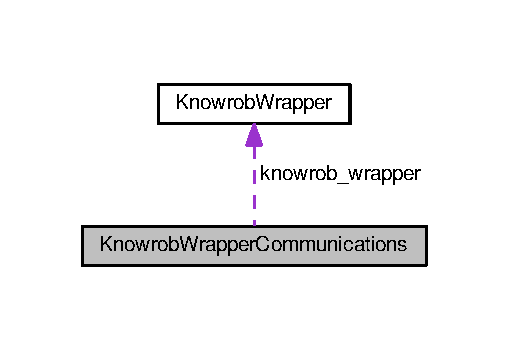
\includegraphics[width=244pt]{classKnowrobWrapperCommunications__coll__graph}
\end{center}
\end{figure}
\subsection*{Public Member Functions}
\begin{DoxyCompactItemize}
\item 
\hyperlink{classKnowrobWrapperCommunications_aa796e3e743aa06c6fd0153cfe4863abd}{Knowrob\-Wrapper\-Communications} ()
\begin{DoxyCompactList}\small\item\em Default constructor. \end{DoxyCompactList}\item 
bool \hyperlink{classKnowrobWrapperCommunications_ad7fae0d25d1f657a5f40df8a4985fb15}{clear\-\_\-user\-\_\-cognitive\-\_\-tests\-\_\-performance\-\_\-records\-\_\-callback} (rapp\-\_\-platform\-\_\-ros\-\_\-communications\-::clear\-User\-Performance\-Cognitve\-Tests\-Srv\-::\-Request \&req, rapp\-\_\-platform\-\_\-ros\-\_\-communications\-::clear\-User\-Performance\-Cognitve\-Tests\-Srv\-::\-Response \&res)
\begin{DoxyCompactList}\small\item\em Serves the clear\-\_\-user\-\_\-cognitive\-\_\-tests\-\_\-performance\-\_\-records R\-O\-S service callback. \end{DoxyCompactList}\item 
bool \hyperlink{classKnowrobWrapperCommunications_a9c598f55161da568022fa1da1406f7e5}{cognitive\-\_\-tests\-\_\-of\-\_\-type\-\_\-callback} (rapp\-\_\-platform\-\_\-ros\-\_\-communications\-::cognitive\-Tests\-Of\-Type\-Srv\-::\-Request \&req, rapp\-\_\-platform\-\_\-ros\-\_\-communications\-::cognitive\-Tests\-Of\-Type\-Srv\-::\-Response \&res)
\begin{DoxyCompactList}\small\item\em Serves the cognitive\-\_\-tests\-\_\-of\-\_\-type R\-O\-S service callback. \end{DoxyCompactList}\item 
bool \hyperlink{classKnowrobWrapperCommunications_af2addeace661115f731721be3a326d8d}{create\-\_\-cognitve\-\_\-tests\-\_\-callback} (rapp\-\_\-platform\-\_\-ros\-\_\-communications\-::create\-Cognitive\-Exercise\-Test\-Srv\-::\-Request \&req, rapp\-\_\-platform\-\_\-ros\-\_\-communications\-::create\-Cognitive\-Exercise\-Test\-Srv\-::\-Response \&res)
\begin{DoxyCompactList}\small\item\em Serves the create\-\_\-cognitve\-\_\-tests R\-O\-S service callback. \end{DoxyCompactList}\item 
bool \hyperlink{classKnowrobWrapperCommunications_a00791d76db809cb09c1f06fd38077c58}{create\-\_\-ontology\-\_\-alias\-\_\-callback} (rapp\-\_\-platform\-\_\-ros\-\_\-communications\-::create\-Ontology\-Alias\-Srv\-::\-Request \&req, rapp\-\_\-platform\-\_\-ros\-\_\-communications\-::create\-Ontology\-Alias\-Srv\-::\-Response \&res)
\begin{DoxyCompactList}\small\item\em Serves the create\-\_\-ontology\-\_\-alias R\-O\-S service callback. \end{DoxyCompactList}\item 
bool \hyperlink{classKnowrobWrapperCommunications_a1b1b3016fe4b7b5321fcbea3a268daa0}{create\-Instance\-Callback} (rapp\-\_\-platform\-\_\-ros\-\_\-communications\-::create\-Instance\-Srv\-::\-Request \&req, rapp\-\_\-platform\-\_\-ros\-\_\-communications\-::create\-Instance\-Srv\-::\-Response \&res)
\begin{DoxyCompactList}\small\item\em Serves the create\-Instance R\-O\-S service callback. \end{DoxyCompactList}\item 
bool \hyperlink{classKnowrobWrapperCommunications_a3be6c8a48ac43fd971d037c7da44ac8c}{dump\-Ontology\-Callback} (rapp\-\_\-platform\-\_\-ros\-\_\-communications\-::ontology\-Load\-Dump\-Srv\-::\-Request \&req, rapp\-\_\-platform\-\_\-ros\-\_\-communications\-::ontology\-Load\-Dump\-Srv\-::\-Response \&res)
\begin{DoxyCompactList}\small\item\em Serves the dump\-Ontology R\-O\-S service callback. \end{DoxyCompactList}\item 
bool \hyperlink{classKnowrobWrapperCommunications_a9323106f5ecb88147604eb12150d92a0}{is\-Sub\-Superclass\-Of\-Callback} (rapp\-\_\-platform\-\_\-ros\-\_\-communications\-::ontology\-Is\-Sub\-Super\-Class\-Of\-Srv\-::\-Request \&req, rapp\-\_\-platform\-\_\-ros\-\_\-communications\-::ontology\-Is\-Sub\-Super\-Class\-Of\-Srv\-::\-Response \&res)
\begin{DoxyCompactList}\small\item\em Serves the is\-Sub\-Superclass\-Of R\-O\-S service callback. \end{DoxyCompactList}\item 
bool \hyperlink{classKnowrobWrapperCommunications_aa7d046afb167ae2fa0658876bafa42ba}{load\-Ontology\-Callback} (rapp\-\_\-platform\-\_\-ros\-\_\-communications\-::ontology\-Load\-Dump\-Srv\-::\-Request \&req, rapp\-\_\-platform\-\_\-ros\-\_\-communications\-::ontology\-Load\-Dump\-Srv\-::\-Response \&res)
\begin{DoxyCompactList}\small\item\em Serves the load\-Ontology R\-O\-S service callback. \end{DoxyCompactList}\item 
bool \hyperlink{classKnowrobWrapperCommunications_a4c2e5ed4bf27e9ae7d722b50d8f607e3}{record\-\_\-user\-\_\-cognitive\-\_\-tests\-\_\-performance\-\_\-callback} (rapp\-\_\-platform\-\_\-ros\-\_\-communications\-::record\-User\-Performance\-Cognitive\-Tests\-Srv\-::\-Request \&req, rapp\-\_\-platform\-\_\-ros\-\_\-communications\-::record\-User\-Performance\-Cognitive\-Tests\-Srv\-::\-Response \&res)
\begin{DoxyCompactList}\small\item\em Serves the record\-\_\-user\-\_\-cognitive\-\_\-tests\-\_\-performance R\-O\-S service callback. \end{DoxyCompactList}\item 
bool \hyperlink{classKnowrobWrapperCommunications_a9d73180cd20c89bbc9e71469a0c53388}{register\-\_\-image\-\_\-object\-\_\-to\-\_\-ontology\-\_\-callback} (rapp\-\_\-platform\-\_\-ros\-\_\-communications\-::register\-Image\-Object\-To\-Ontology\-Srv\-::\-Request \&req, rapp\-\_\-platform\-\_\-ros\-\_\-communications\-::register\-Image\-Object\-To\-Ontology\-Srv\-::\-Response \&res)
\begin{DoxyCompactList}\small\item\em Serves the register\-\_\-image\-\_\-object\-\_\-to\-\_\-ontology R\-O\-S service callback. \end{DoxyCompactList}\item 
bool \hyperlink{classKnowrobWrapperCommunications_aa149f2929cb7b5cda2c7615e07d4a5cc}{retract\-\_\-user\-\_\-ontology\-\_\-alias\-\_\-callback} (rapp\-\_\-platform\-\_\-ros\-\_\-communications\-::retract\-User\-Ontology\-Alias\-Srv\-::\-Request \&req, rapp\-\_\-platform\-\_\-ros\-\_\-communications\-::retract\-User\-Ontology\-Alias\-Srv\-::\-Response \&res)
\begin{DoxyCompactList}\small\item\em Serves the retract\-\_\-user\-\_\-ontology\-\_\-alias R\-O\-S service callback. \end{DoxyCompactList}\item 
bool \hyperlink{classKnowrobWrapperCommunications_a4d0118b6016bd1df21abca155ae9b423}{subclasses\-Of\-Callback} (rapp\-\_\-platform\-\_\-ros\-\_\-communications\-::ontology\-Sub\-Super\-Classes\-Of\-Srv\-::\-Request \&req, rapp\-\_\-platform\-\_\-ros\-\_\-communications\-::ontology\-Sub\-Super\-Classes\-Of\-Srv\-::\-Response \&res)
\begin{DoxyCompactList}\small\item\em Serves the subclasses\-Of R\-O\-S service callback. \end{DoxyCompactList}\item 
bool \hyperlink{classKnowrobWrapperCommunications_aa2f78a0238538e4c047ee7d931969219}{superclasses\-Of\-Callback} (rapp\-\_\-platform\-\_\-ros\-\_\-communications\-::ontology\-Sub\-Super\-Classes\-Of\-Srv\-::\-Request \&req, rapp\-\_\-platform\-\_\-ros\-\_\-communications\-::ontology\-Sub\-Super\-Classes\-Of\-Srv\-::\-Response \&res)
\begin{DoxyCompactList}\small\item\em Serves the superlasses\-Of R\-O\-S service callback. \end{DoxyCompactList}\item 
bool \hyperlink{classKnowrobWrapperCommunications_aa0de5d8940bd5b84b44306eb193d4adc}{user\-\_\-instances\-\_\-of\-\_\-class\-\_\-callback} (rapp\-\_\-platform\-\_\-ros\-\_\-communications\-::return\-User\-Instances\-Of\-Class\-Srv\-::\-Request \&req, rapp\-\_\-platform\-\_\-ros\-\_\-communications\-::return\-User\-Instances\-Of\-Class\-Srv\-::\-Response \&res)
\begin{DoxyCompactList}\small\item\em Serves the user\-\_\-instances\-\_\-of\-\_\-class R\-O\-S service callback. \end{DoxyCompactList}\item 
bool \hyperlink{classKnowrobWrapperCommunications_a956d4705d0234c0ed13179aff5897b30}{user\-\_\-performance\-\_\-cognitve\-\_\-tests\-\_\-callback} (rapp\-\_\-platform\-\_\-ros\-\_\-communications\-::user\-Performance\-Cognitve\-Tests\-Srv\-::\-Request \&req, rapp\-\_\-platform\-\_\-ros\-\_\-communications\-::user\-Performance\-Cognitve\-Tests\-Srv\-::\-Response \&res)
\begin{DoxyCompactList}\small\item\em Serves the user\-\_\-performance\-\_\-cognitve\-\_\-tests R\-O\-S service callback. \end{DoxyCompactList}\end{DoxyCompactItemize}
\subsection*{Private Attributes}
\begin{DoxyCompactItemize}
\item 
ros\-::\-Service\-Server \hyperlink{classKnowrobWrapperCommunications_afc3b9e19e7d950f62dd29222a779ea30}{clear\-\_\-user\-\_\-cognitive\-\_\-tests\-\_\-performance\-\_\-records\-\_\-service\-\_\-}
\item 
std\-::string \hyperlink{classKnowrobWrapperCommunications_ac555026ed985ed7cc020b1f0c33ae054}{clear\-\_\-user\-\_\-cognitive\-\_\-tests\-\_\-performance\-\_\-records\-\_\-topic\-\_\-}
\item 
ros\-::\-Service\-Server \hyperlink{classKnowrobWrapperCommunications_ac2498f2732057c72fc4bbc0ffcb29c7b}{cognitive\-\_\-tests\-\_\-of\-\_\-type\-\_\-service\-\_\-}
\item 
std\-::string \hyperlink{classKnowrobWrapperCommunications_a40ffe00f1d833232faf6d265bd5276b8}{cognitive\-\_\-tests\-\_\-of\-\_\-type\-\_\-topic\-\_\-}
\item 
ros\-::\-Service\-Server \hyperlink{classKnowrobWrapperCommunications_a835254476d15a2c224069d4ff5ae0ce5}{create\-\_\-cognitve\-\_\-tests\-\_\-service\-\_\-}
\item 
std\-::string \hyperlink{classKnowrobWrapperCommunications_ab90753196ac931da226e940346162255}{create\-\_\-cognitve\-\_\-tests\-\_\-topic\-\_\-}
\item 
ros\-::\-Service\-Server \hyperlink{classKnowrobWrapperCommunications_a522e95f339e854d9202d212885cd542e}{create\-\_\-ontology\-\_\-alias\-\_\-service\-\_\-}
\item 
std\-::string \hyperlink{classKnowrobWrapperCommunications_ae3bf27737520a9ee4ce0ec43bffb15e4}{create\-\_\-ontology\-\_\-alias\-\_\-topic\-\_\-}
\item 
ros\-::\-Service\-Server \hyperlink{classKnowrobWrapperCommunications_a2be003e4372235aba8c48f08ee160bdb}{create\-Instance\-Service\-\_\-}
\item 
std\-::string \hyperlink{classKnowrobWrapperCommunications_ae4d64655c9da3ad80b79197f7cc761ef}{create\-Instance\-Service\-Topic\-\_\-}
\item 
ros\-::\-Service\-Server \hyperlink{classKnowrobWrapperCommunications_af0ad3b846b7441ed1256ab14501689dc}{dump\-Ontology\-Service\-\_\-}
\item 
std\-::string \hyperlink{classKnowrobWrapperCommunications_a581d7bbfc90299d80e504c59df83510d}{dump\-Ontology\-Service\-Topic\-\_\-}
\item 
ros\-::\-Service\-Server \hyperlink{classKnowrobWrapperCommunications_a9b20954a7983e1a0f842161d06555484}{is\-\_\-subsuperclass\-\_\-of\-\_\-service\-\_\-}
\item 
std\-::string \hyperlink{classKnowrobWrapperCommunications_ab7d3b5d16106e51472f8fcb771be96aa}{is\-\_\-subsuperclass\-\_\-of\-\_\-service\-\_\-topic\-\_\-}
\item 
\hyperlink{classKnowrobWrapper}{Knowrob\-Wrapper} \hyperlink{classKnowrobWrapperCommunications_a6f4d52c56702c85b21b96df9caf95f46}{knowrob\-\_\-wrapper}
\item 
ros\-::\-Service\-Server \hyperlink{classKnowrobWrapperCommunications_aa0e819f7420b8e9f5315b9cfaac53bf4}{load\-Ontology\-Service\-\_\-}
\item 
std\-::string \hyperlink{classKnowrobWrapperCommunications_a6d5a84e3b69d020b5e11595a2ae871b5}{load\-Ontology\-Service\-Topic\-\_\-}
\item 
ros\-::\-Node\-Handle \hyperlink{classKnowrobWrapperCommunications_afe35871d80ea79c6446d2bdf39ba6204}{nh\-\_\-}
\item 
ros\-::\-Service\-Server \hyperlink{classKnowrobWrapperCommunications_a17e239928cdfac593e27e015e70ad376}{record\-\_\-user\-\_\-cognitive\-\_\-tests\-\_\-performance\-\_\-service\-\_\-}
\item 
std\-::string \hyperlink{classKnowrobWrapperCommunications_a1e44e99eba8f3a2fb196a9d215cec89c}{record\-\_\-user\-\_\-cognitive\-\_\-tests\-\_\-performance\-\_\-topic\-\_\-}
\item 
ros\-::\-Service\-Server \hyperlink{classKnowrobWrapperCommunications_a80d24d312e258d4b546573d4eaeb6a16}{register\-\_\-image\-\_\-object\-\_\-to\-\_\-ontology\-\_\-service\-\_\-}
\item 
std\-::string \hyperlink{classKnowrobWrapperCommunications_aeeadfeab13814b51e78182bb52358303}{register\-\_\-image\-\_\-object\-\_\-to\-\_\-ontology\-\_\-topic\-\_\-}
\item 
ros\-::\-Service\-Server \hyperlink{classKnowrobWrapperCommunications_a281262d96049a59096a5a29fbaac77d2}{retract\-\_\-user\-\_\-ontology\-\_\-alias\-\_\-service\-\_\-}
\item 
std\-::string \hyperlink{classKnowrobWrapperCommunications_afde9fb500053dd1ac1605af6728f03f0}{retract\-\_\-user\-\_\-ontology\-\_\-alias\-\_\-topic\-\_\-}
\item 
ros\-::\-Service\-Server \hyperlink{classKnowrobWrapperCommunications_aa694eb182b48822ca845e34096b17ad4}{subclasses\-\_\-of\-\_\-service\-\_\-}
\item 
std\-::string \hyperlink{classKnowrobWrapperCommunications_afbce99db77d63a6a052ebf7041cbc232}{subclasses\-\_\-of\-\_\-service\-\_\-topic\-\_\-}
\item 
ros\-::\-Service\-Server \hyperlink{classKnowrobWrapperCommunications_a4f20e98c56e5dd773524db0518ea55a2}{superclasses\-\_\-of\-\_\-service\-\_\-}
\item 
std\-::string \hyperlink{classKnowrobWrapperCommunications_aeed7bc627032586a30f7405ed7450dc2}{superclasses\-\_\-of\-\_\-service\-\_\-topic\-\_\-}
\item 
ros\-::\-Service\-Server \hyperlink{classKnowrobWrapperCommunications_a135ffaafe3229f5208de0622430fa9b6}{user\-\_\-instances\-\_\-of\-\_\-class\-\_\-service\-\_\-}
\item 
std\-::string \hyperlink{classKnowrobWrapperCommunications_aa6f2cc5d4d4dd17b22f490a89387dc35}{user\-\_\-instances\-\_\-of\-\_\-class\-\_\-topic\-\_\-}
\item 
ros\-::\-Service\-Server \hyperlink{classKnowrobWrapperCommunications_acc4fabd8a1dd21309c01b03e4c5129e5}{user\-\_\-performance\-\_\-cognitve\-\_\-tests\-\_\-service\-\_\-}
\item 
std\-::string \hyperlink{classKnowrobWrapperCommunications_a8304cf850b658cabf9a8494b6b745f1b}{user\-\_\-performance\-\_\-cognitve\-\_\-tests\-\_\-topic\-\_\-}
\end{DoxyCompactItemize}


\subsection{Detailed Description}
Class \hyperlink{classKnowrobWrapperCommunications}{Knowrob\-Wrapper\-Communications} uptakes the task of handling the R\-O\-S service callbacks. 

Definition at line 28 of file knowrob\-\_\-wrapper\-\_\-communications.\-h.



\subsection{Constructor \& Destructor Documentation}
\hypertarget{classKnowrobWrapperCommunications_aa796e3e743aa06c6fd0153cfe4863abd}{\index{Knowrob\-Wrapper\-Communications@{Knowrob\-Wrapper\-Communications}!Knowrob\-Wrapper\-Communications@{Knowrob\-Wrapper\-Communications}}
\index{Knowrob\-Wrapper\-Communications@{Knowrob\-Wrapper\-Communications}!KnowrobWrapperCommunications@{Knowrob\-Wrapper\-Communications}}
\subsubsection[{Knowrob\-Wrapper\-Communications}]{\setlength{\rightskip}{0pt plus 5cm}Knowrob\-Wrapper\-Communications\-::\-Knowrob\-Wrapper\-Communications (
\begin{DoxyParamCaption}
{}
\end{DoxyParamCaption}
)}}\label{classKnowrobWrapperCommunications_aa796e3e743aa06c6fd0153cfe4863abd}


Default constructor. 

Default constructor Waits for services it depends on and declares the knowrob wrapper services callbacks. 

Definition at line 28 of file knowrob\-\_\-wrapper\-\_\-communications.\-cpp.



\subsection{Member Function Documentation}
\hypertarget{classKnowrobWrapperCommunications_ad7fae0d25d1f657a5f40df8a4985fb15}{\index{Knowrob\-Wrapper\-Communications@{Knowrob\-Wrapper\-Communications}!clear\-\_\-user\-\_\-cognitive\-\_\-tests\-\_\-performance\-\_\-records\-\_\-callback@{clear\-\_\-user\-\_\-cognitive\-\_\-tests\-\_\-performance\-\_\-records\-\_\-callback}}
\index{clear\-\_\-user\-\_\-cognitive\-\_\-tests\-\_\-performance\-\_\-records\-\_\-callback@{clear\-\_\-user\-\_\-cognitive\-\_\-tests\-\_\-performance\-\_\-records\-\_\-callback}!KnowrobWrapperCommunications@{Knowrob\-Wrapper\-Communications}}
\subsubsection[{clear\-\_\-user\-\_\-cognitive\-\_\-tests\-\_\-performance\-\_\-records\-\_\-callback}]{\setlength{\rightskip}{0pt plus 5cm}bool Knowrob\-Wrapper\-Communications\-::clear\-\_\-user\-\_\-cognitive\-\_\-tests\-\_\-performance\-\_\-records\-\_\-callback (
\begin{DoxyParamCaption}
\item[{rapp\-\_\-platform\-\_\-ros\-\_\-communications\-::clear\-User\-Performance\-Cognitve\-Tests\-Srv\-::\-Request \&}]{req, }
\item[{rapp\-\_\-platform\-\_\-ros\-\_\-communications\-::clear\-User\-Performance\-Cognitve\-Tests\-Srv\-::\-Response \&}]{res}
\end{DoxyParamCaption}
)}}\label{classKnowrobWrapperCommunications_ad7fae0d25d1f657a5f40df8a4985fb15}


Serves the clear\-\_\-user\-\_\-cognitive\-\_\-tests\-\_\-performance\-\_\-records R\-O\-S service callback. 


\begin{DoxyParams}{Parameters}
{\em req} & \mbox{[}rapp\-\_\-platform\-\_\-ros\-\_\-communications\-::clear\-User\-Performance\-Cognitve\-Tests\-Srv\-::\-Request\&\mbox{]} The R\-O\-S service request \\
\hline
{\em res} & \mbox{[}rapp\-\_\-platform\-\_\-ros\-\_\-communications\-::clear\-User\-Performance\-Cognitve\-Tests\-Srv\-::\-Response\&\mbox{]} The R\-O\-S service response \\
\hline
\end{DoxyParams}
\begin{DoxyReturn}{Returns}
bool -\/ The success status of the call 
\end{DoxyReturn}


Definition at line 331 of file knowrob\-\_\-wrapper\-\_\-communications.\-cpp.

\hypertarget{classKnowrobWrapperCommunications_a9c598f55161da568022fa1da1406f7e5}{\index{Knowrob\-Wrapper\-Communications@{Knowrob\-Wrapper\-Communications}!cognitive\-\_\-tests\-\_\-of\-\_\-type\-\_\-callback@{cognitive\-\_\-tests\-\_\-of\-\_\-type\-\_\-callback}}
\index{cognitive\-\_\-tests\-\_\-of\-\_\-type\-\_\-callback@{cognitive\-\_\-tests\-\_\-of\-\_\-type\-\_\-callback}!KnowrobWrapperCommunications@{Knowrob\-Wrapper\-Communications}}
\subsubsection[{cognitive\-\_\-tests\-\_\-of\-\_\-type\-\_\-callback}]{\setlength{\rightskip}{0pt plus 5cm}bool Knowrob\-Wrapper\-Communications\-::cognitive\-\_\-tests\-\_\-of\-\_\-type\-\_\-callback (
\begin{DoxyParamCaption}
\item[{rapp\-\_\-platform\-\_\-ros\-\_\-communications\-::cognitive\-Tests\-Of\-Type\-Srv\-::\-Request \&}]{req, }
\item[{rapp\-\_\-platform\-\_\-ros\-\_\-communications\-::cognitive\-Tests\-Of\-Type\-Srv\-::\-Response \&}]{res}
\end{DoxyParamCaption}
)}}\label{classKnowrobWrapperCommunications_a9c598f55161da568022fa1da1406f7e5}


Serves the cognitive\-\_\-tests\-\_\-of\-\_\-type R\-O\-S service callback. 


\begin{DoxyParams}{Parameters}
{\em req} & \mbox{[}rapp\-\_\-platform\-\_\-ros\-\_\-communications\-::cognitive\-Tests\-Of\-Type\-Srv\-::\-Request\&\mbox{]} The R\-O\-S service request \\
\hline
{\em res} & \mbox{[}rapp\-\_\-platform\-\_\-ros\-\_\-communications\-::cognitive\-Tests\-Of\-Type\-Srv\-::\-Response\&\mbox{]} The R\-O\-S service response \\
\hline
\end{DoxyParams}
\begin{DoxyReturn}{Returns}
bool -\/ The success status of the call 
\end{DoxyReturn}


Definition at line 303 of file knowrob\-\_\-wrapper\-\_\-communications.\-cpp.

\hypertarget{classKnowrobWrapperCommunications_af2addeace661115f731721be3a326d8d}{\index{Knowrob\-Wrapper\-Communications@{Knowrob\-Wrapper\-Communications}!create\-\_\-cognitve\-\_\-tests\-\_\-callback@{create\-\_\-cognitve\-\_\-tests\-\_\-callback}}
\index{create\-\_\-cognitve\-\_\-tests\-\_\-callback@{create\-\_\-cognitve\-\_\-tests\-\_\-callback}!KnowrobWrapperCommunications@{Knowrob\-Wrapper\-Communications}}
\subsubsection[{create\-\_\-cognitve\-\_\-tests\-\_\-callback}]{\setlength{\rightskip}{0pt plus 5cm}bool Knowrob\-Wrapper\-Communications\-::create\-\_\-cognitve\-\_\-tests\-\_\-callback (
\begin{DoxyParamCaption}
\item[{rapp\-\_\-platform\-\_\-ros\-\_\-communications\-::create\-Cognitive\-Exercise\-Test\-Srv\-::\-Request \&}]{req, }
\item[{rapp\-\_\-platform\-\_\-ros\-\_\-communications\-::create\-Cognitive\-Exercise\-Test\-Srv\-::\-Response \&}]{res}
\end{DoxyParamCaption}
)}}\label{classKnowrobWrapperCommunications_af2addeace661115f731721be3a326d8d}


Serves the create\-\_\-cognitve\-\_\-tests R\-O\-S service callback. 


\begin{DoxyParams}{Parameters}
{\em req} & \mbox{[}rapp\-\_\-platform\-\_\-ros\-\_\-communications\-::create\-Cognitive\-Exercise\-Test\-Srv\-::\-Request\&\mbox{]} The R\-O\-S service request \\
\hline
{\em res} & \mbox{[}rapp\-\_\-platform\-\_\-ros\-\_\-communications\-::create\-Cognitive\-Exercise\-Test\-Srv\-::\-Response\&\mbox{]} The R\-O\-S service response \\
\hline
\end{DoxyParams}
\begin{DoxyReturn}{Returns}
bool -\/ The success status of the call 
\end{DoxyReturn}


Definition at line 289 of file knowrob\-\_\-wrapper\-\_\-communications.\-cpp.

\hypertarget{classKnowrobWrapperCommunications_a00791d76db809cb09c1f06fd38077c58}{\index{Knowrob\-Wrapper\-Communications@{Knowrob\-Wrapper\-Communications}!create\-\_\-ontology\-\_\-alias\-\_\-callback@{create\-\_\-ontology\-\_\-alias\-\_\-callback}}
\index{create\-\_\-ontology\-\_\-alias\-\_\-callback@{create\-\_\-ontology\-\_\-alias\-\_\-callback}!KnowrobWrapperCommunications@{Knowrob\-Wrapper\-Communications}}
\subsubsection[{create\-\_\-ontology\-\_\-alias\-\_\-callback}]{\setlength{\rightskip}{0pt plus 5cm}bool Knowrob\-Wrapper\-Communications\-::create\-\_\-ontology\-\_\-alias\-\_\-callback (
\begin{DoxyParamCaption}
\item[{rapp\-\_\-platform\-\_\-ros\-\_\-communications\-::create\-Ontology\-Alias\-Srv\-::\-Request \&}]{req, }
\item[{rapp\-\_\-platform\-\_\-ros\-\_\-communications\-::create\-Ontology\-Alias\-Srv\-::\-Response \&}]{res}
\end{DoxyParamCaption}
)}}\label{classKnowrobWrapperCommunications_a00791d76db809cb09c1f06fd38077c58}


Serves the create\-\_\-ontology\-\_\-alias R\-O\-S service callback. 


\begin{DoxyParams}{Parameters}
{\em req} & \mbox{[}rapp\-\_\-platform\-\_\-ros\-\_\-communications\-::create\-Ontology\-Alias\-Srv\-::\-Request\&\mbox{]} The R\-O\-S service request \\
\hline
{\em res} & \mbox{[}rapp\-\_\-platform\-\_\-ros\-\_\-communications\-::create\-Ontology\-Alias\-Srv\-::\-Response\&\mbox{]} The R\-O\-S service response \\
\hline
\end{DoxyParams}
\begin{DoxyReturn}{Returns}
bool -\/ The success status of the call 
\end{DoxyReturn}


Definition at line 247 of file knowrob\-\_\-wrapper\-\_\-communications.\-cpp.

\hypertarget{classKnowrobWrapperCommunications_a1b1b3016fe4b7b5321fcbea3a268daa0}{\index{Knowrob\-Wrapper\-Communications@{Knowrob\-Wrapper\-Communications}!create\-Instance\-Callback@{create\-Instance\-Callback}}
\index{create\-Instance\-Callback@{create\-Instance\-Callback}!KnowrobWrapperCommunications@{Knowrob\-Wrapper\-Communications}}
\subsubsection[{create\-Instance\-Callback}]{\setlength{\rightskip}{0pt plus 5cm}bool Knowrob\-Wrapper\-Communications\-::create\-Instance\-Callback (
\begin{DoxyParamCaption}
\item[{rapp\-\_\-platform\-\_\-ros\-\_\-communications\-::create\-Instance\-Srv\-::\-Request \&}]{req, }
\item[{rapp\-\_\-platform\-\_\-ros\-\_\-communications\-::create\-Instance\-Srv\-::\-Response \&}]{res}
\end{DoxyParamCaption}
)}}\label{classKnowrobWrapperCommunications_a1b1b3016fe4b7b5321fcbea3a268daa0}


Serves the create\-Instance R\-O\-S service callback. 


\begin{DoxyParams}{Parameters}
{\em req} & \mbox{[}rapp\-\_\-platform\-\_\-ros\-\_\-communications\-::create\-Instance\-Srv\-::\-Request\&\mbox{]} The R\-O\-S service request \\
\hline
{\em res} & \mbox{[}rapp\-\_\-platform\-\_\-ros\-\_\-communications\-::create\-Instance\-Srv\-::\-Response\&\mbox{]} The R\-O\-S service response \\
\hline
\end{DoxyParams}
\begin{DoxyReturn}{Returns}
bool -\/ The success status of the call 
\end{DoxyReturn}


Definition at line 205 of file knowrob\-\_\-wrapper\-\_\-communications.\-cpp.

\hypertarget{classKnowrobWrapperCommunications_a3be6c8a48ac43fd971d037c7da44ac8c}{\index{Knowrob\-Wrapper\-Communications@{Knowrob\-Wrapper\-Communications}!dump\-Ontology\-Callback@{dump\-Ontology\-Callback}}
\index{dump\-Ontology\-Callback@{dump\-Ontology\-Callback}!KnowrobWrapperCommunications@{Knowrob\-Wrapper\-Communications}}
\subsubsection[{dump\-Ontology\-Callback}]{\setlength{\rightskip}{0pt plus 5cm}bool Knowrob\-Wrapper\-Communications\-::dump\-Ontology\-Callback (
\begin{DoxyParamCaption}
\item[{rapp\-\_\-platform\-\_\-ros\-\_\-communications\-::ontology\-Load\-Dump\-Srv\-::\-Request \&}]{req, }
\item[{rapp\-\_\-platform\-\_\-ros\-\_\-communications\-::ontology\-Load\-Dump\-Srv\-::\-Response \&}]{res}
\end{DoxyParamCaption}
)}}\label{classKnowrobWrapperCommunications_a3be6c8a48ac43fd971d037c7da44ac8c}


Serves the dump\-Ontology R\-O\-S service callback. 


\begin{DoxyParams}{Parameters}
{\em req} & \mbox{[}rapp\-\_\-platform\-\_\-ros\-\_\-communications\-::ontology\-Load\-Dump\-Srv\-::\-Request\&\mbox{]} The R\-O\-S service request \\
\hline
{\em res} & \mbox{[}rapp\-\_\-platform\-\_\-ros\-\_\-communications\-::ontology\-Load\-Dump\-Srv\-::\-Response\&\mbox{]} The R\-O\-S service response \\
\hline
\end{DoxyParams}
\begin{DoxyReturn}{Returns}
bool -\/ The success status of the call 
\end{DoxyReturn}


Definition at line 219 of file knowrob\-\_\-wrapper\-\_\-communications.\-cpp.

\hypertarget{classKnowrobWrapperCommunications_a9323106f5ecb88147604eb12150d92a0}{\index{Knowrob\-Wrapper\-Communications@{Knowrob\-Wrapper\-Communications}!is\-Sub\-Superclass\-Of\-Callback@{is\-Sub\-Superclass\-Of\-Callback}}
\index{is\-Sub\-Superclass\-Of\-Callback@{is\-Sub\-Superclass\-Of\-Callback}!KnowrobWrapperCommunications@{Knowrob\-Wrapper\-Communications}}
\subsubsection[{is\-Sub\-Superclass\-Of\-Callback}]{\setlength{\rightskip}{0pt plus 5cm}bool Knowrob\-Wrapper\-Communications\-::is\-Sub\-Superclass\-Of\-Callback (
\begin{DoxyParamCaption}
\item[{rapp\-\_\-platform\-\_\-ros\-\_\-communications\-::ontology\-Is\-Sub\-Super\-Class\-Of\-Srv\-::\-Request \&}]{req, }
\item[{rapp\-\_\-platform\-\_\-ros\-\_\-communications\-::ontology\-Is\-Sub\-Super\-Class\-Of\-Srv\-::\-Response \&}]{res}
\end{DoxyParamCaption}
)}}\label{classKnowrobWrapperCommunications_a9323106f5ecb88147604eb12150d92a0}


Serves the is\-Sub\-Superclass\-Of R\-O\-S service callback. 


\begin{DoxyParams}{Parameters}
{\em req} & \mbox{[}rapp\-\_\-platform\-\_\-ros\-\_\-communications\-::ontology\-Is\-Sub\-Super\-Class\-Of\-Srv\-::\-Request\&\mbox{]} The R\-O\-S service request \\
\hline
{\em res} & \mbox{[}rapp\-\_\-platform\-\_\-ros\-\_\-communications\-::ontology\-Is\-Sub\-Super\-Class\-Of\-Srv\-::\-Response\&\mbox{]} The R\-O\-S service response \\
\hline
\end{DoxyParams}
\begin{DoxyReturn}{Returns}
bool -\/ The success status of the call 
\end{DoxyReturn}


Definition at line 191 of file knowrob\-\_\-wrapper\-\_\-communications.\-cpp.

\hypertarget{classKnowrobWrapperCommunications_aa7d046afb167ae2fa0658876bafa42ba}{\index{Knowrob\-Wrapper\-Communications@{Knowrob\-Wrapper\-Communications}!load\-Ontology\-Callback@{load\-Ontology\-Callback}}
\index{load\-Ontology\-Callback@{load\-Ontology\-Callback}!KnowrobWrapperCommunications@{Knowrob\-Wrapper\-Communications}}
\subsubsection[{load\-Ontology\-Callback}]{\setlength{\rightskip}{0pt plus 5cm}bool Knowrob\-Wrapper\-Communications\-::load\-Ontology\-Callback (
\begin{DoxyParamCaption}
\item[{rapp\-\_\-platform\-\_\-ros\-\_\-communications\-::ontology\-Load\-Dump\-Srv\-::\-Request \&}]{req, }
\item[{rapp\-\_\-platform\-\_\-ros\-\_\-communications\-::ontology\-Load\-Dump\-Srv\-::\-Response \&}]{res}
\end{DoxyParamCaption}
)}}\label{classKnowrobWrapperCommunications_aa7d046afb167ae2fa0658876bafa42ba}


Serves the load\-Ontology R\-O\-S service callback. 


\begin{DoxyParams}{Parameters}
{\em req} & \mbox{[}rapp\-\_\-platform\-\_\-ros\-\_\-communications\-::ontology\-Load\-Dump\-Srv\-::\-Request\&\mbox{]} The R\-O\-S service request \\
\hline
{\em res} & \mbox{[}rapp\-\_\-platform\-\_\-ros\-\_\-communications\-::ontology\-Load\-Dump\-Srv\-::\-Response\&\mbox{]} The R\-O\-S service response \\
\hline
\end{DoxyParams}
\begin{DoxyReturn}{Returns}
bool -\/ The success status of the call 
\end{DoxyReturn}


Definition at line 233 of file knowrob\-\_\-wrapper\-\_\-communications.\-cpp.

\hypertarget{classKnowrobWrapperCommunications_a4c2e5ed4bf27e9ae7d722b50d8f607e3}{\index{Knowrob\-Wrapper\-Communications@{Knowrob\-Wrapper\-Communications}!record\-\_\-user\-\_\-cognitive\-\_\-tests\-\_\-performance\-\_\-callback@{record\-\_\-user\-\_\-cognitive\-\_\-tests\-\_\-performance\-\_\-callback}}
\index{record\-\_\-user\-\_\-cognitive\-\_\-tests\-\_\-performance\-\_\-callback@{record\-\_\-user\-\_\-cognitive\-\_\-tests\-\_\-performance\-\_\-callback}!KnowrobWrapperCommunications@{Knowrob\-Wrapper\-Communications}}
\subsubsection[{record\-\_\-user\-\_\-cognitive\-\_\-tests\-\_\-performance\-\_\-callback}]{\setlength{\rightskip}{0pt plus 5cm}bool Knowrob\-Wrapper\-Communications\-::record\-\_\-user\-\_\-cognitive\-\_\-tests\-\_\-performance\-\_\-callback (
\begin{DoxyParamCaption}
\item[{rapp\-\_\-platform\-\_\-ros\-\_\-communications\-::record\-User\-Performance\-Cognitive\-Tests\-Srv\-::\-Request \&}]{req, }
\item[{rapp\-\_\-platform\-\_\-ros\-\_\-communications\-::record\-User\-Performance\-Cognitive\-Tests\-Srv\-::\-Response \&}]{res}
\end{DoxyParamCaption}
)}}\label{classKnowrobWrapperCommunications_a4c2e5ed4bf27e9ae7d722b50d8f607e3}


Serves the record\-\_\-user\-\_\-cognitive\-\_\-tests\-\_\-performance R\-O\-S service callback. 


\begin{DoxyParams}{Parameters}
{\em req} & \mbox{[}rapp\-\_\-platform\-\_\-ros\-\_\-communications\-::record\-User\-Performance\-Cognitive\-Tests\-Srv\-::\-Request\&\mbox{]} The R\-O\-S service request \\
\hline
{\em res} & \mbox{[}rapp\-\_\-platform\-\_\-ros\-\_\-communications\-::record\-User\-Performance\-Cognitive\-Tests\-Srv\-::\-Response\&\mbox{]} The R\-O\-S service response \\
\hline
\end{DoxyParams}
\begin{DoxyReturn}{Returns}
bool -\/ The success status of the call 
\end{DoxyReturn}


Definition at line 317 of file knowrob\-\_\-wrapper\-\_\-communications.\-cpp.

\hypertarget{classKnowrobWrapperCommunications_a9d73180cd20c89bbc9e71469a0c53388}{\index{Knowrob\-Wrapper\-Communications@{Knowrob\-Wrapper\-Communications}!register\-\_\-image\-\_\-object\-\_\-to\-\_\-ontology\-\_\-callback@{register\-\_\-image\-\_\-object\-\_\-to\-\_\-ontology\-\_\-callback}}
\index{register\-\_\-image\-\_\-object\-\_\-to\-\_\-ontology\-\_\-callback@{register\-\_\-image\-\_\-object\-\_\-to\-\_\-ontology\-\_\-callback}!KnowrobWrapperCommunications@{Knowrob\-Wrapper\-Communications}}
\subsubsection[{register\-\_\-image\-\_\-object\-\_\-to\-\_\-ontology\-\_\-callback}]{\setlength{\rightskip}{0pt plus 5cm}bool Knowrob\-Wrapper\-Communications\-::register\-\_\-image\-\_\-object\-\_\-to\-\_\-ontology\-\_\-callback (
\begin{DoxyParamCaption}
\item[{rapp\-\_\-platform\-\_\-ros\-\_\-communications\-::register\-Image\-Object\-To\-Ontology\-Srv\-::\-Request \&}]{req, }
\item[{rapp\-\_\-platform\-\_\-ros\-\_\-communications\-::register\-Image\-Object\-To\-Ontology\-Srv\-::\-Response \&}]{res}
\end{DoxyParamCaption}
)}}\label{classKnowrobWrapperCommunications_a9d73180cd20c89bbc9e71469a0c53388}


Serves the register\-\_\-image\-\_\-object\-\_\-to\-\_\-ontology R\-O\-S service callback. 


\begin{DoxyParams}{Parameters}
{\em req} & \mbox{[}rapp\-\_\-platform\-\_\-ros\-\_\-communications\-::register\-Image\-To\-Ontology\-Srv\-::\-Request\&\mbox{]} The R\-O\-S service request \\
\hline
{\em res} & \mbox{[}rapp\-\_\-platform\-\_\-ros\-\_\-communications\-::register\-Image\-To\-Ontology\-Srv\-::\-Response\&\mbox{]} The R\-O\-S service response \\
\hline
\end{DoxyParams}
\begin{DoxyReturn}{Returns}
bool -\/ The success status of the call 
\end{DoxyReturn}


Definition at line 359 of file knowrob\-\_\-wrapper\-\_\-communications.\-cpp.

\hypertarget{classKnowrobWrapperCommunications_aa149f2929cb7b5cda2c7615e07d4a5cc}{\index{Knowrob\-Wrapper\-Communications@{Knowrob\-Wrapper\-Communications}!retract\-\_\-user\-\_\-ontology\-\_\-alias\-\_\-callback@{retract\-\_\-user\-\_\-ontology\-\_\-alias\-\_\-callback}}
\index{retract\-\_\-user\-\_\-ontology\-\_\-alias\-\_\-callback@{retract\-\_\-user\-\_\-ontology\-\_\-alias\-\_\-callback}!KnowrobWrapperCommunications@{Knowrob\-Wrapper\-Communications}}
\subsubsection[{retract\-\_\-user\-\_\-ontology\-\_\-alias\-\_\-callback}]{\setlength{\rightskip}{0pt plus 5cm}bool Knowrob\-Wrapper\-Communications\-::retract\-\_\-user\-\_\-ontology\-\_\-alias\-\_\-callback (
\begin{DoxyParamCaption}
\item[{rapp\-\_\-platform\-\_\-ros\-\_\-communications\-::retract\-User\-Ontology\-Alias\-Srv\-::\-Request \&}]{req, }
\item[{rapp\-\_\-platform\-\_\-ros\-\_\-communications\-::retract\-User\-Ontology\-Alias\-Srv\-::\-Response \&}]{res}
\end{DoxyParamCaption}
)}}\label{classKnowrobWrapperCommunications_aa149f2929cb7b5cda2c7615e07d4a5cc}


Serves the retract\-\_\-user\-\_\-ontology\-\_\-alias R\-O\-S service callback. 


\begin{DoxyParams}{Parameters}
{\em req} & \mbox{[}rapp\-\_\-platform\-\_\-ros\-\_\-communications\-::retract\-User\-Ontology\-Alias\-Srv\-::\-Request\&\mbox{]} The R\-O\-S service request \\
\hline
{\em res} & \mbox{[}rapp\-\_\-platform\-\_\-ros\-\_\-communications\-::retract\-User\-Ontology\-Alias\-Srv\-::\-Response\&\mbox{]} The R\-O\-S service response \\
\hline
\end{DoxyParams}
\begin{DoxyReturn}{Returns}
bool -\/ The success status of the call 
\end{DoxyReturn}


Definition at line 345 of file knowrob\-\_\-wrapper\-\_\-communications.\-cpp.

\hypertarget{classKnowrobWrapperCommunications_a4d0118b6016bd1df21abca155ae9b423}{\index{Knowrob\-Wrapper\-Communications@{Knowrob\-Wrapper\-Communications}!subclasses\-Of\-Callback@{subclasses\-Of\-Callback}}
\index{subclasses\-Of\-Callback@{subclasses\-Of\-Callback}!KnowrobWrapperCommunications@{Knowrob\-Wrapper\-Communications}}
\subsubsection[{subclasses\-Of\-Callback}]{\setlength{\rightskip}{0pt plus 5cm}bool Knowrob\-Wrapper\-Communications\-::subclasses\-Of\-Callback (
\begin{DoxyParamCaption}
\item[{rapp\-\_\-platform\-\_\-ros\-\_\-communications\-::ontology\-Sub\-Super\-Classes\-Of\-Srv\-::\-Request \&}]{req, }
\item[{rapp\-\_\-platform\-\_\-ros\-\_\-communications\-::ontology\-Sub\-Super\-Classes\-Of\-Srv\-::\-Response \&}]{res}
\end{DoxyParamCaption}
)}}\label{classKnowrobWrapperCommunications_a4d0118b6016bd1df21abca155ae9b423}


Serves the subclasses\-Of R\-O\-S service callback. 


\begin{DoxyParams}{Parameters}
{\em req} & \mbox{[}rapp\-\_\-platform\-\_\-ros\-\_\-communications\-::ontology\-Sub\-Super\-Classes\-Of\-Srv\-::\-Request\&\mbox{]} The R\-O\-S service request \\
\hline
{\em res} & \mbox{[}rapp\-\_\-platform\-\_\-ros\-\_\-communications\-::ontology\-Sub\-Super\-Classes\-Of\-Srv\-::\-Response\&\mbox{]} The R\-O\-S service response \\
\hline
\end{DoxyParams}
\begin{DoxyReturn}{Returns}
bool -\/ The success status of the call 
\end{DoxyReturn}


Definition at line 163 of file knowrob\-\_\-wrapper\-\_\-communications.\-cpp.

\hypertarget{classKnowrobWrapperCommunications_aa2f78a0238538e4c047ee7d931969219}{\index{Knowrob\-Wrapper\-Communications@{Knowrob\-Wrapper\-Communications}!superclasses\-Of\-Callback@{superclasses\-Of\-Callback}}
\index{superclasses\-Of\-Callback@{superclasses\-Of\-Callback}!KnowrobWrapperCommunications@{Knowrob\-Wrapper\-Communications}}
\subsubsection[{superclasses\-Of\-Callback}]{\setlength{\rightskip}{0pt plus 5cm}bool Knowrob\-Wrapper\-Communications\-::superclasses\-Of\-Callback (
\begin{DoxyParamCaption}
\item[{rapp\-\_\-platform\-\_\-ros\-\_\-communications\-::ontology\-Sub\-Super\-Classes\-Of\-Srv\-::\-Request \&}]{req, }
\item[{rapp\-\_\-platform\-\_\-ros\-\_\-communications\-::ontology\-Sub\-Super\-Classes\-Of\-Srv\-::\-Response \&}]{res}
\end{DoxyParamCaption}
)}}\label{classKnowrobWrapperCommunications_aa2f78a0238538e4c047ee7d931969219}


Serves the superlasses\-Of R\-O\-S service callback. 


\begin{DoxyParams}{Parameters}
{\em req} & \mbox{[}rapp\-\_\-platform\-\_\-ros\-\_\-communications\-::ontology\-Sub\-Super\-Classes\-Of\-Srv\-::\-Request\&\mbox{]} The R\-O\-S service request \\
\hline
{\em res} & \mbox{[}rapp\-\_\-platform\-\_\-ros\-\_\-communications\-::ontology\-Sub\-Super\-Classes\-Of\-Srv\-::\-Response\&\mbox{]} The R\-O\-S service response \\
\hline
\end{DoxyParams}
\begin{DoxyReturn}{Returns}
bool -\/ The success status of the call 
\end{DoxyReturn}


Definition at line 177 of file knowrob\-\_\-wrapper\-\_\-communications.\-cpp.

\hypertarget{classKnowrobWrapperCommunications_aa0de5d8940bd5b84b44306eb193d4adc}{\index{Knowrob\-Wrapper\-Communications@{Knowrob\-Wrapper\-Communications}!user\-\_\-instances\-\_\-of\-\_\-class\-\_\-callback@{user\-\_\-instances\-\_\-of\-\_\-class\-\_\-callback}}
\index{user\-\_\-instances\-\_\-of\-\_\-class\-\_\-callback@{user\-\_\-instances\-\_\-of\-\_\-class\-\_\-callback}!KnowrobWrapperCommunications@{Knowrob\-Wrapper\-Communications}}
\subsubsection[{user\-\_\-instances\-\_\-of\-\_\-class\-\_\-callback}]{\setlength{\rightskip}{0pt plus 5cm}bool Knowrob\-Wrapper\-Communications\-::user\-\_\-instances\-\_\-of\-\_\-class\-\_\-callback (
\begin{DoxyParamCaption}
\item[{rapp\-\_\-platform\-\_\-ros\-\_\-communications\-::return\-User\-Instances\-Of\-Class\-Srv\-::\-Request \&}]{req, }
\item[{rapp\-\_\-platform\-\_\-ros\-\_\-communications\-::return\-User\-Instances\-Of\-Class\-Srv\-::\-Response \&}]{res}
\end{DoxyParamCaption}
)}}\label{classKnowrobWrapperCommunications_aa0de5d8940bd5b84b44306eb193d4adc}


Serves the user\-\_\-instances\-\_\-of\-\_\-class R\-O\-S service callback. 


\begin{DoxyParams}{Parameters}
{\em req} & \mbox{[}rapp\-\_\-platform\-\_\-ros\-\_\-communications\-::return\-User\-Instances\-Of\-Class\-Srv\-::\-Request\&\mbox{]} The R\-O\-S service request \\
\hline
{\em res} & \mbox{[}rapp\-\_\-platform\-\_\-ros\-\_\-communications\-::return\-User\-Instances\-Of\-Class\-Srv\-::\-Response\&\mbox{]} The R\-O\-S service response \\
\hline
\end{DoxyParams}
\begin{DoxyReturn}{Returns}
bool -\/ The success status of the call 
\end{DoxyReturn}


Definition at line 261 of file knowrob\-\_\-wrapper\-\_\-communications.\-cpp.

\hypertarget{classKnowrobWrapperCommunications_a956d4705d0234c0ed13179aff5897b30}{\index{Knowrob\-Wrapper\-Communications@{Knowrob\-Wrapper\-Communications}!user\-\_\-performance\-\_\-cognitve\-\_\-tests\-\_\-callback@{user\-\_\-performance\-\_\-cognitve\-\_\-tests\-\_\-callback}}
\index{user\-\_\-performance\-\_\-cognitve\-\_\-tests\-\_\-callback@{user\-\_\-performance\-\_\-cognitve\-\_\-tests\-\_\-callback}!KnowrobWrapperCommunications@{Knowrob\-Wrapper\-Communications}}
\subsubsection[{user\-\_\-performance\-\_\-cognitve\-\_\-tests\-\_\-callback}]{\setlength{\rightskip}{0pt plus 5cm}bool Knowrob\-Wrapper\-Communications\-::user\-\_\-performance\-\_\-cognitve\-\_\-tests\-\_\-callback (
\begin{DoxyParamCaption}
\item[{rapp\-\_\-platform\-\_\-ros\-\_\-communications\-::user\-Performance\-Cognitve\-Tests\-Srv\-::\-Request \&}]{req, }
\item[{rapp\-\_\-platform\-\_\-ros\-\_\-communications\-::user\-Performance\-Cognitve\-Tests\-Srv\-::\-Response \&}]{res}
\end{DoxyParamCaption}
)}}\label{classKnowrobWrapperCommunications_a956d4705d0234c0ed13179aff5897b30}


Serves the user\-\_\-performance\-\_\-cognitve\-\_\-tests R\-O\-S service callback. 


\begin{DoxyParams}{Parameters}
{\em req} & \mbox{[}rapp\-\_\-platform\-\_\-ros\-\_\-communications\-::user\-Performance\-Cognitve\-Tests\-Srv\-::\-Request\&\mbox{]} The R\-O\-S service request \\
\hline
{\em res} & \mbox{[}rapp\-\_\-platform\-\_\-ros\-\_\-communications\-::user\-Performance\-Cognitve\-Tests\-Srv\-::\-Response\&\mbox{]} The R\-O\-S service response \\
\hline
\end{DoxyParams}
\begin{DoxyReturn}{Returns}
bool -\/ The success status of the call 
\end{DoxyReturn}


Definition at line 275 of file knowrob\-\_\-wrapper\-\_\-communications.\-cpp.



\subsection{Member Data Documentation}
\hypertarget{classKnowrobWrapperCommunications_afc3b9e19e7d950f62dd29222a779ea30}{\index{Knowrob\-Wrapper\-Communications@{Knowrob\-Wrapper\-Communications}!clear\-\_\-user\-\_\-cognitive\-\_\-tests\-\_\-performance\-\_\-records\-\_\-service\-\_\-@{clear\-\_\-user\-\_\-cognitive\-\_\-tests\-\_\-performance\-\_\-records\-\_\-service\-\_\-}}
\index{clear\-\_\-user\-\_\-cognitive\-\_\-tests\-\_\-performance\-\_\-records\-\_\-service\-\_\-@{clear\-\_\-user\-\_\-cognitive\-\_\-tests\-\_\-performance\-\_\-records\-\_\-service\-\_\-}!KnowrobWrapperCommunications@{Knowrob\-Wrapper\-Communications}}
\subsubsection[{clear\-\_\-user\-\_\-cognitive\-\_\-tests\-\_\-performance\-\_\-records\-\_\-service\-\_\-}]{\setlength{\rightskip}{0pt plus 5cm}ros\-::\-Service\-Server Knowrob\-Wrapper\-Communications\-::clear\-\_\-user\-\_\-cognitive\-\_\-tests\-\_\-performance\-\_\-records\-\_\-service\-\_\-\hspace{0.3cm}{\ttfamily [private]}}}\label{classKnowrobWrapperCommunications_afc3b9e19e7d950f62dd29222a779ea30}
Member variable holding the clear\-\_\-user\-\_\-cognitive\-\_\-tests\-\_\-performance\-\_\-records R\-O\-S service topic 

Definition at line 99 of file knowrob\-\_\-wrapper\-\_\-communications.\-h.

\hypertarget{classKnowrobWrapperCommunications_ac555026ed985ed7cc020b1f0c33ae054}{\index{Knowrob\-Wrapper\-Communications@{Knowrob\-Wrapper\-Communications}!clear\-\_\-user\-\_\-cognitive\-\_\-tests\-\_\-performance\-\_\-records\-\_\-topic\-\_\-@{clear\-\_\-user\-\_\-cognitive\-\_\-tests\-\_\-performance\-\_\-records\-\_\-topic\-\_\-}}
\index{clear\-\_\-user\-\_\-cognitive\-\_\-tests\-\_\-performance\-\_\-records\-\_\-topic\-\_\-@{clear\-\_\-user\-\_\-cognitive\-\_\-tests\-\_\-performance\-\_\-records\-\_\-topic\-\_\-}!KnowrobWrapperCommunications@{Knowrob\-Wrapper\-Communications}}
\subsubsection[{clear\-\_\-user\-\_\-cognitive\-\_\-tests\-\_\-performance\-\_\-records\-\_\-topic\-\_\-}]{\setlength{\rightskip}{0pt plus 5cm}std\-::string Knowrob\-Wrapper\-Communications\-::clear\-\_\-user\-\_\-cognitive\-\_\-tests\-\_\-performance\-\_\-records\-\_\-topic\-\_\-\hspace{0.3cm}{\ttfamily [private]}}}\label{classKnowrobWrapperCommunications_ac555026ed985ed7cc020b1f0c33ae054}
The retract\-\_\-user\-\_\-ontology\-\_\-alias service server 

Definition at line 101 of file knowrob\-\_\-wrapper\-\_\-communications.\-h.

\hypertarget{classKnowrobWrapperCommunications_ac2498f2732057c72fc4bbc0ffcb29c7b}{\index{Knowrob\-Wrapper\-Communications@{Knowrob\-Wrapper\-Communications}!cognitive\-\_\-tests\-\_\-of\-\_\-type\-\_\-service\-\_\-@{cognitive\-\_\-tests\-\_\-of\-\_\-type\-\_\-service\-\_\-}}
\index{cognitive\-\_\-tests\-\_\-of\-\_\-type\-\_\-service\-\_\-@{cognitive\-\_\-tests\-\_\-of\-\_\-type\-\_\-service\-\_\-}!KnowrobWrapperCommunications@{Knowrob\-Wrapper\-Communications}}
\subsubsection[{cognitive\-\_\-tests\-\_\-of\-\_\-type\-\_\-service\-\_\-}]{\setlength{\rightskip}{0pt plus 5cm}ros\-::\-Service\-Server Knowrob\-Wrapper\-Communications\-::cognitive\-\_\-tests\-\_\-of\-\_\-type\-\_\-service\-\_\-\hspace{0.3cm}{\ttfamily [private]}}}\label{classKnowrobWrapperCommunications_ac2498f2732057c72fc4bbc0ffcb29c7b}
Member variable holding the cognitive\-\_\-tests\-\_\-of\-\_\-type R\-O\-S service topic 

Definition at line 89 of file knowrob\-\_\-wrapper\-\_\-communications.\-h.

\hypertarget{classKnowrobWrapperCommunications_a40ffe00f1d833232faf6d265bd5276b8}{\index{Knowrob\-Wrapper\-Communications@{Knowrob\-Wrapper\-Communications}!cognitive\-\_\-tests\-\_\-of\-\_\-type\-\_\-topic\-\_\-@{cognitive\-\_\-tests\-\_\-of\-\_\-type\-\_\-topic\-\_\-}}
\index{cognitive\-\_\-tests\-\_\-of\-\_\-type\-\_\-topic\-\_\-@{cognitive\-\_\-tests\-\_\-of\-\_\-type\-\_\-topic\-\_\-}!KnowrobWrapperCommunications@{Knowrob\-Wrapper\-Communications}}
\subsubsection[{cognitive\-\_\-tests\-\_\-of\-\_\-type\-\_\-topic\-\_\-}]{\setlength{\rightskip}{0pt plus 5cm}std\-::string Knowrob\-Wrapper\-Communications\-::cognitive\-\_\-tests\-\_\-of\-\_\-type\-\_\-topic\-\_\-\hspace{0.3cm}{\ttfamily [private]}}}\label{classKnowrobWrapperCommunications_a40ffe00f1d833232faf6d265bd5276b8}
The record\-\_\-user\-\_\-cognitive\-\_\-tests\-\_\-performance service server 

Definition at line 91 of file knowrob\-\_\-wrapper\-\_\-communications.\-h.

\hypertarget{classKnowrobWrapperCommunications_a835254476d15a2c224069d4ff5ae0ce5}{\index{Knowrob\-Wrapper\-Communications@{Knowrob\-Wrapper\-Communications}!create\-\_\-cognitve\-\_\-tests\-\_\-service\-\_\-@{create\-\_\-cognitve\-\_\-tests\-\_\-service\-\_\-}}
\index{create\-\_\-cognitve\-\_\-tests\-\_\-service\-\_\-@{create\-\_\-cognitve\-\_\-tests\-\_\-service\-\_\-}!KnowrobWrapperCommunications@{Knowrob\-Wrapper\-Communications}}
\subsubsection[{create\-\_\-cognitve\-\_\-tests\-\_\-service\-\_\-}]{\setlength{\rightskip}{0pt plus 5cm}ros\-::\-Service\-Server Knowrob\-Wrapper\-Communications\-::create\-\_\-cognitve\-\_\-tests\-\_\-service\-\_\-\hspace{0.3cm}{\ttfamily [private]}}}\label{classKnowrobWrapperCommunications_a835254476d15a2c224069d4ff5ae0ce5}
Member variable holding the create\-\_\-cognitve\-\_\-tests R\-O\-S service topic 

Definition at line 84 of file knowrob\-\_\-wrapper\-\_\-communications.\-h.

\hypertarget{classKnowrobWrapperCommunications_ab90753196ac931da226e940346162255}{\index{Knowrob\-Wrapper\-Communications@{Knowrob\-Wrapper\-Communications}!create\-\_\-cognitve\-\_\-tests\-\_\-topic\-\_\-@{create\-\_\-cognitve\-\_\-tests\-\_\-topic\-\_\-}}
\index{create\-\_\-cognitve\-\_\-tests\-\_\-topic\-\_\-@{create\-\_\-cognitve\-\_\-tests\-\_\-topic\-\_\-}!KnowrobWrapperCommunications@{Knowrob\-Wrapper\-Communications}}
\subsubsection[{create\-\_\-cognitve\-\_\-tests\-\_\-topic\-\_\-}]{\setlength{\rightskip}{0pt plus 5cm}std\-::string Knowrob\-Wrapper\-Communications\-::create\-\_\-cognitve\-\_\-tests\-\_\-topic\-\_\-\hspace{0.3cm}{\ttfamily [private]}}}\label{classKnowrobWrapperCommunications_ab90753196ac931da226e940346162255}
The cognitive\-\_\-tests\-\_\-of\-\_\-type service server 

Definition at line 86 of file knowrob\-\_\-wrapper\-\_\-communications.\-h.

\hypertarget{classKnowrobWrapperCommunications_a522e95f339e854d9202d212885cd542e}{\index{Knowrob\-Wrapper\-Communications@{Knowrob\-Wrapper\-Communications}!create\-\_\-ontology\-\_\-alias\-\_\-service\-\_\-@{create\-\_\-ontology\-\_\-alias\-\_\-service\-\_\-}}
\index{create\-\_\-ontology\-\_\-alias\-\_\-service\-\_\-@{create\-\_\-ontology\-\_\-alias\-\_\-service\-\_\-}!KnowrobWrapperCommunications@{Knowrob\-Wrapper\-Communications}}
\subsubsection[{create\-\_\-ontology\-\_\-alias\-\_\-service\-\_\-}]{\setlength{\rightskip}{0pt plus 5cm}ros\-::\-Service\-Server Knowrob\-Wrapper\-Communications\-::create\-\_\-ontology\-\_\-alias\-\_\-service\-\_\-\hspace{0.3cm}{\ttfamily [private]}}}\label{classKnowrobWrapperCommunications_a522e95f339e854d9202d212885cd542e}
Member variable holding the create\-\_\-ontology\-\_\-alias R\-O\-S service topic 

Definition at line 74 of file knowrob\-\_\-wrapper\-\_\-communications.\-h.

\hypertarget{classKnowrobWrapperCommunications_ae3bf27737520a9ee4ce0ec43bffb15e4}{\index{Knowrob\-Wrapper\-Communications@{Knowrob\-Wrapper\-Communications}!create\-\_\-ontology\-\_\-alias\-\_\-topic\-\_\-@{create\-\_\-ontology\-\_\-alias\-\_\-topic\-\_\-}}
\index{create\-\_\-ontology\-\_\-alias\-\_\-topic\-\_\-@{create\-\_\-ontology\-\_\-alias\-\_\-topic\-\_\-}!KnowrobWrapperCommunications@{Knowrob\-Wrapper\-Communications}}
\subsubsection[{create\-\_\-ontology\-\_\-alias\-\_\-topic\-\_\-}]{\setlength{\rightskip}{0pt plus 5cm}std\-::string Knowrob\-Wrapper\-Communications\-::create\-\_\-ontology\-\_\-alias\-\_\-topic\-\_\-\hspace{0.3cm}{\ttfamily [private]}}}\label{classKnowrobWrapperCommunications_ae3bf27737520a9ee4ce0ec43bffb15e4}
The user\-\_\-performance\-\_\-cognitve\-\_\-tests service server 

Definition at line 76 of file knowrob\-\_\-wrapper\-\_\-communications.\-h.

\hypertarget{classKnowrobWrapperCommunications_a2be003e4372235aba8c48f08ee160bdb}{\index{Knowrob\-Wrapper\-Communications@{Knowrob\-Wrapper\-Communications}!create\-Instance\-Service\-\_\-@{create\-Instance\-Service\-\_\-}}
\index{create\-Instance\-Service\-\_\-@{create\-Instance\-Service\-\_\-}!KnowrobWrapperCommunications@{Knowrob\-Wrapper\-Communications}}
\subsubsection[{create\-Instance\-Service\-\_\-}]{\setlength{\rightskip}{0pt plus 5cm}ros\-::\-Service\-Server Knowrob\-Wrapper\-Communications\-::create\-Instance\-Service\-\_\-\hspace{0.3cm}{\ttfamily [private]}}}\label{classKnowrobWrapperCommunications_a2be003e4372235aba8c48f08ee160bdb}
Member variable holding the create\-Instance\-Service\-Topic R\-O\-S service topic 

Definition at line 54 of file knowrob\-\_\-wrapper\-\_\-communications.\-h.

\hypertarget{classKnowrobWrapperCommunications_ae4d64655c9da3ad80b79197f7cc761ef}{\index{Knowrob\-Wrapper\-Communications@{Knowrob\-Wrapper\-Communications}!create\-Instance\-Service\-Topic\-\_\-@{create\-Instance\-Service\-Topic\-\_\-}}
\index{create\-Instance\-Service\-Topic\-\_\-@{create\-Instance\-Service\-Topic\-\_\-}!KnowrobWrapperCommunications@{Knowrob\-Wrapper\-Communications}}
\subsubsection[{create\-Instance\-Service\-Topic\-\_\-}]{\setlength{\rightskip}{0pt plus 5cm}std\-::string Knowrob\-Wrapper\-Communications\-::create\-Instance\-Service\-Topic\-\_\-\hspace{0.3cm}{\ttfamily [private]}}}\label{classKnowrobWrapperCommunications_ae4d64655c9da3ad80b79197f7cc761ef}
The dump\-Ontology\-Service service server 

Definition at line 56 of file knowrob\-\_\-wrapper\-\_\-communications.\-h.

\hypertarget{classKnowrobWrapperCommunications_af0ad3b846b7441ed1256ab14501689dc}{\index{Knowrob\-Wrapper\-Communications@{Knowrob\-Wrapper\-Communications}!dump\-Ontology\-Service\-\_\-@{dump\-Ontology\-Service\-\_\-}}
\index{dump\-Ontology\-Service\-\_\-@{dump\-Ontology\-Service\-\_\-}!KnowrobWrapperCommunications@{Knowrob\-Wrapper\-Communications}}
\subsubsection[{dump\-Ontology\-Service\-\_\-}]{\setlength{\rightskip}{0pt plus 5cm}ros\-::\-Service\-Server Knowrob\-Wrapper\-Communications\-::dump\-Ontology\-Service\-\_\-\hspace{0.3cm}{\ttfamily [private]}}}\label{classKnowrobWrapperCommunications_af0ad3b846b7441ed1256ab14501689dc}
Member variable holding the dump\-Ontology\-Service\-Topic R\-O\-S service topic 

Definition at line 59 of file knowrob\-\_\-wrapper\-\_\-communications.\-h.

\hypertarget{classKnowrobWrapperCommunications_a581d7bbfc90299d80e504c59df83510d}{\index{Knowrob\-Wrapper\-Communications@{Knowrob\-Wrapper\-Communications}!dump\-Ontology\-Service\-Topic\-\_\-@{dump\-Ontology\-Service\-Topic\-\_\-}}
\index{dump\-Ontology\-Service\-Topic\-\_\-@{dump\-Ontology\-Service\-Topic\-\_\-}!KnowrobWrapperCommunications@{Knowrob\-Wrapper\-Communications}}
\subsubsection[{dump\-Ontology\-Service\-Topic\-\_\-}]{\setlength{\rightskip}{0pt plus 5cm}std\-::string Knowrob\-Wrapper\-Communications\-::dump\-Ontology\-Service\-Topic\-\_\-\hspace{0.3cm}{\ttfamily [private]}}}\label{classKnowrobWrapperCommunications_a581d7bbfc90299d80e504c59df83510d}
The load\-Ontology\-Service service server 

Definition at line 61 of file knowrob\-\_\-wrapper\-\_\-communications.\-h.

\hypertarget{classKnowrobWrapperCommunications_a9b20954a7983e1a0f842161d06555484}{\index{Knowrob\-Wrapper\-Communications@{Knowrob\-Wrapper\-Communications}!is\-\_\-subsuperclass\-\_\-of\-\_\-service\-\_\-@{is\-\_\-subsuperclass\-\_\-of\-\_\-service\-\_\-}}
\index{is\-\_\-subsuperclass\-\_\-of\-\_\-service\-\_\-@{is\-\_\-subsuperclass\-\_\-of\-\_\-service\-\_\-}!KnowrobWrapperCommunications@{Knowrob\-Wrapper\-Communications}}
\subsubsection[{is\-\_\-subsuperclass\-\_\-of\-\_\-service\-\_\-}]{\setlength{\rightskip}{0pt plus 5cm}ros\-::\-Service\-Server Knowrob\-Wrapper\-Communications\-::is\-\_\-subsuperclass\-\_\-of\-\_\-service\-\_\-\hspace{0.3cm}{\ttfamily [private]}}}\label{classKnowrobWrapperCommunications_a9b20954a7983e1a0f842161d06555484}
Member variable holding the is\-\_\-subsuperclass R\-O\-S service topic 

Definition at line 49 of file knowrob\-\_\-wrapper\-\_\-communications.\-h.

\hypertarget{classKnowrobWrapperCommunications_ab7d3b5d16106e51472f8fcb771be96aa}{\index{Knowrob\-Wrapper\-Communications@{Knowrob\-Wrapper\-Communications}!is\-\_\-subsuperclass\-\_\-of\-\_\-service\-\_\-topic\-\_\-@{is\-\_\-subsuperclass\-\_\-of\-\_\-service\-\_\-topic\-\_\-}}
\index{is\-\_\-subsuperclass\-\_\-of\-\_\-service\-\_\-topic\-\_\-@{is\-\_\-subsuperclass\-\_\-of\-\_\-service\-\_\-topic\-\_\-}!KnowrobWrapperCommunications@{Knowrob\-Wrapper\-Communications}}
\subsubsection[{is\-\_\-subsuperclass\-\_\-of\-\_\-service\-\_\-topic\-\_\-}]{\setlength{\rightskip}{0pt plus 5cm}std\-::string Knowrob\-Wrapper\-Communications\-::is\-\_\-subsuperclass\-\_\-of\-\_\-service\-\_\-topic\-\_\-\hspace{0.3cm}{\ttfamily [private]}}}\label{classKnowrobWrapperCommunications_ab7d3b5d16106e51472f8fcb771be96aa}
The create\-Instance\-Service service server 

Definition at line 51 of file knowrob\-\_\-wrapper\-\_\-communications.\-h.

\hypertarget{classKnowrobWrapperCommunications_a6f4d52c56702c85b21b96df9caf95f46}{\index{Knowrob\-Wrapper\-Communications@{Knowrob\-Wrapper\-Communications}!knowrob\-\_\-wrapper@{knowrob\-\_\-wrapper}}
\index{knowrob\-\_\-wrapper@{knowrob\-\_\-wrapper}!KnowrobWrapperCommunications@{Knowrob\-Wrapper\-Communications}}
\subsubsection[{knowrob\-\_\-wrapper}]{\setlength{\rightskip}{0pt plus 5cm}{\bf Knowrob\-Wrapper} Knowrob\-Wrapper\-Communications\-::knowrob\-\_\-wrapper\hspace{0.3cm}{\ttfamily [private]}}}\label{classKnowrobWrapperCommunications_a6f4d52c56702c85b21b96df9caf95f46}
The subclasses\-\_\-of service server 

Definition at line 35 of file knowrob\-\_\-wrapper\-\_\-communications.\-h.

\hypertarget{classKnowrobWrapperCommunications_aa0e819f7420b8e9f5315b9cfaac53bf4}{\index{Knowrob\-Wrapper\-Communications@{Knowrob\-Wrapper\-Communications}!load\-Ontology\-Service\-\_\-@{load\-Ontology\-Service\-\_\-}}
\index{load\-Ontology\-Service\-\_\-@{load\-Ontology\-Service\-\_\-}!KnowrobWrapperCommunications@{Knowrob\-Wrapper\-Communications}}
\subsubsection[{load\-Ontology\-Service\-\_\-}]{\setlength{\rightskip}{0pt plus 5cm}ros\-::\-Service\-Server Knowrob\-Wrapper\-Communications\-::load\-Ontology\-Service\-\_\-\hspace{0.3cm}{\ttfamily [private]}}}\label{classKnowrobWrapperCommunications_aa0e819f7420b8e9f5315b9cfaac53bf4}
Member variable holding the load\-Ontology\-Service\-Topic R\-O\-S service topic 

Definition at line 64 of file knowrob\-\_\-wrapper\-\_\-communications.\-h.

\hypertarget{classKnowrobWrapperCommunications_a6d5a84e3b69d020b5e11595a2ae871b5}{\index{Knowrob\-Wrapper\-Communications@{Knowrob\-Wrapper\-Communications}!load\-Ontology\-Service\-Topic\-\_\-@{load\-Ontology\-Service\-Topic\-\_\-}}
\index{load\-Ontology\-Service\-Topic\-\_\-@{load\-Ontology\-Service\-Topic\-\_\-}!KnowrobWrapperCommunications@{Knowrob\-Wrapper\-Communications}}
\subsubsection[{load\-Ontology\-Service\-Topic\-\_\-}]{\setlength{\rightskip}{0pt plus 5cm}std\-::string Knowrob\-Wrapper\-Communications\-::load\-Ontology\-Service\-Topic\-\_\-\hspace{0.3cm}{\ttfamily [private]}}}\label{classKnowrobWrapperCommunications_a6d5a84e3b69d020b5e11595a2ae871b5}
The user\-\_\-instances\-\_\-of\-\_\-class service server 

Definition at line 66 of file knowrob\-\_\-wrapper\-\_\-communications.\-h.

\hypertarget{classKnowrobWrapperCommunications_afe35871d80ea79c6446d2bdf39ba6204}{\index{Knowrob\-Wrapper\-Communications@{Knowrob\-Wrapper\-Communications}!nh\-\_\-@{nh\-\_\-}}
\index{nh\-\_\-@{nh\-\_\-}!KnowrobWrapperCommunications@{Knowrob\-Wrapper\-Communications}}
\subsubsection[{nh\-\_\-}]{\setlength{\rightskip}{0pt plus 5cm}ros\-::\-Node\-Handle Knowrob\-Wrapper\-Communications\-::nh\-\_\-\hspace{0.3cm}{\ttfamily [private]}}}\label{classKnowrobWrapperCommunications_afe35871d80ea79c6446d2bdf39ba6204}
$<$ The R\-O\-S node handle Object of type knowrob\-\_\-wrapper 

Definition at line 32 of file knowrob\-\_\-wrapper\-\_\-communications.\-h.

\hypertarget{classKnowrobWrapperCommunications_a17e239928cdfac593e27e015e70ad376}{\index{Knowrob\-Wrapper\-Communications@{Knowrob\-Wrapper\-Communications}!record\-\_\-user\-\_\-cognitive\-\_\-tests\-\_\-performance\-\_\-service\-\_\-@{record\-\_\-user\-\_\-cognitive\-\_\-tests\-\_\-performance\-\_\-service\-\_\-}}
\index{record\-\_\-user\-\_\-cognitive\-\_\-tests\-\_\-performance\-\_\-service\-\_\-@{record\-\_\-user\-\_\-cognitive\-\_\-tests\-\_\-performance\-\_\-service\-\_\-}!KnowrobWrapperCommunications@{Knowrob\-Wrapper\-Communications}}
\subsubsection[{record\-\_\-user\-\_\-cognitive\-\_\-tests\-\_\-performance\-\_\-service\-\_\-}]{\setlength{\rightskip}{0pt plus 5cm}ros\-::\-Service\-Server Knowrob\-Wrapper\-Communications\-::record\-\_\-user\-\_\-cognitive\-\_\-tests\-\_\-performance\-\_\-service\-\_\-\hspace{0.3cm}{\ttfamily [private]}}}\label{classKnowrobWrapperCommunications_a17e239928cdfac593e27e015e70ad376}
Member variable holding the record\-\_\-user\-\_\-cognitive\-\_\-tests\-\_\-performance R\-O\-S service topic 

Definition at line 94 of file knowrob\-\_\-wrapper\-\_\-communications.\-h.

\hypertarget{classKnowrobWrapperCommunications_a1e44e99eba8f3a2fb196a9d215cec89c}{\index{Knowrob\-Wrapper\-Communications@{Knowrob\-Wrapper\-Communications}!record\-\_\-user\-\_\-cognitive\-\_\-tests\-\_\-performance\-\_\-topic\-\_\-@{record\-\_\-user\-\_\-cognitive\-\_\-tests\-\_\-performance\-\_\-topic\-\_\-}}
\index{record\-\_\-user\-\_\-cognitive\-\_\-tests\-\_\-performance\-\_\-topic\-\_\-@{record\-\_\-user\-\_\-cognitive\-\_\-tests\-\_\-performance\-\_\-topic\-\_\-}!KnowrobWrapperCommunications@{Knowrob\-Wrapper\-Communications}}
\subsubsection[{record\-\_\-user\-\_\-cognitive\-\_\-tests\-\_\-performance\-\_\-topic\-\_\-}]{\setlength{\rightskip}{0pt plus 5cm}std\-::string Knowrob\-Wrapper\-Communications\-::record\-\_\-user\-\_\-cognitive\-\_\-tests\-\_\-performance\-\_\-topic\-\_\-\hspace{0.3cm}{\ttfamily [private]}}}\label{classKnowrobWrapperCommunications_a1e44e99eba8f3a2fb196a9d215cec89c}
The clear\-\_\-user\-\_\-cognitive\-\_\-tests\-\_\-performance\-\_\-records service server 

Definition at line 96 of file knowrob\-\_\-wrapper\-\_\-communications.\-h.

\hypertarget{classKnowrobWrapperCommunications_a80d24d312e258d4b546573d4eaeb6a16}{\index{Knowrob\-Wrapper\-Communications@{Knowrob\-Wrapper\-Communications}!register\-\_\-image\-\_\-object\-\_\-to\-\_\-ontology\-\_\-service\-\_\-@{register\-\_\-image\-\_\-object\-\_\-to\-\_\-ontology\-\_\-service\-\_\-}}
\index{register\-\_\-image\-\_\-object\-\_\-to\-\_\-ontology\-\_\-service\-\_\-@{register\-\_\-image\-\_\-object\-\_\-to\-\_\-ontology\-\_\-service\-\_\-}!KnowrobWrapperCommunications@{Knowrob\-Wrapper\-Communications}}
\subsubsection[{register\-\_\-image\-\_\-object\-\_\-to\-\_\-ontology\-\_\-service\-\_\-}]{\setlength{\rightskip}{0pt plus 5cm}ros\-::\-Service\-Server Knowrob\-Wrapper\-Communications\-::register\-\_\-image\-\_\-object\-\_\-to\-\_\-ontology\-\_\-service\-\_\-\hspace{0.3cm}{\ttfamily [private]}}}\label{classKnowrobWrapperCommunications_a80d24d312e258d4b546573d4eaeb6a16}
Member variable holding the register\-\_\-image\-\_\-object\-\_\-to\-\_\-ontology R\-O\-S service topic 

Definition at line 109 of file knowrob\-\_\-wrapper\-\_\-communications.\-h.

\hypertarget{classKnowrobWrapperCommunications_aeeadfeab13814b51e78182bb52358303}{\index{Knowrob\-Wrapper\-Communications@{Knowrob\-Wrapper\-Communications}!register\-\_\-image\-\_\-object\-\_\-to\-\_\-ontology\-\_\-topic\-\_\-@{register\-\_\-image\-\_\-object\-\_\-to\-\_\-ontology\-\_\-topic\-\_\-}}
\index{register\-\_\-image\-\_\-object\-\_\-to\-\_\-ontology\-\_\-topic\-\_\-@{register\-\_\-image\-\_\-object\-\_\-to\-\_\-ontology\-\_\-topic\-\_\-}!KnowrobWrapperCommunications@{Knowrob\-Wrapper\-Communications}}
\subsubsection[{register\-\_\-image\-\_\-object\-\_\-to\-\_\-ontology\-\_\-topic\-\_\-}]{\setlength{\rightskip}{0pt plus 5cm}std\-::string Knowrob\-Wrapper\-Communications\-::register\-\_\-image\-\_\-object\-\_\-to\-\_\-ontology\-\_\-topic\-\_\-\hspace{0.3cm}{\ttfamily [private]}}}\label{classKnowrobWrapperCommunications_aeeadfeab13814b51e78182bb52358303}


Definition at line 111 of file knowrob\-\_\-wrapper\-\_\-communications.\-h.

\hypertarget{classKnowrobWrapperCommunications_a281262d96049a59096a5a29fbaac77d2}{\index{Knowrob\-Wrapper\-Communications@{Knowrob\-Wrapper\-Communications}!retract\-\_\-user\-\_\-ontology\-\_\-alias\-\_\-service\-\_\-@{retract\-\_\-user\-\_\-ontology\-\_\-alias\-\_\-service\-\_\-}}
\index{retract\-\_\-user\-\_\-ontology\-\_\-alias\-\_\-service\-\_\-@{retract\-\_\-user\-\_\-ontology\-\_\-alias\-\_\-service\-\_\-}!KnowrobWrapperCommunications@{Knowrob\-Wrapper\-Communications}}
\subsubsection[{retract\-\_\-user\-\_\-ontology\-\_\-alias\-\_\-service\-\_\-}]{\setlength{\rightskip}{0pt plus 5cm}ros\-::\-Service\-Server Knowrob\-Wrapper\-Communications\-::retract\-\_\-user\-\_\-ontology\-\_\-alias\-\_\-service\-\_\-\hspace{0.3cm}{\ttfamily [private]}}}\label{classKnowrobWrapperCommunications_a281262d96049a59096a5a29fbaac77d2}
Member variable holding the retract\-\_\-user\-\_\-ontology\-\_\-alias R\-O\-S service topic 

Definition at line 104 of file knowrob\-\_\-wrapper\-\_\-communications.\-h.

\hypertarget{classKnowrobWrapperCommunications_afde9fb500053dd1ac1605af6728f03f0}{\index{Knowrob\-Wrapper\-Communications@{Knowrob\-Wrapper\-Communications}!retract\-\_\-user\-\_\-ontology\-\_\-alias\-\_\-topic\-\_\-@{retract\-\_\-user\-\_\-ontology\-\_\-alias\-\_\-topic\-\_\-}}
\index{retract\-\_\-user\-\_\-ontology\-\_\-alias\-\_\-topic\-\_\-@{retract\-\_\-user\-\_\-ontology\-\_\-alias\-\_\-topic\-\_\-}!KnowrobWrapperCommunications@{Knowrob\-Wrapper\-Communications}}
\subsubsection[{retract\-\_\-user\-\_\-ontology\-\_\-alias\-\_\-topic\-\_\-}]{\setlength{\rightskip}{0pt plus 5cm}std\-::string Knowrob\-Wrapper\-Communications\-::retract\-\_\-user\-\_\-ontology\-\_\-alias\-\_\-topic\-\_\-\hspace{0.3cm}{\ttfamily [private]}}}\label{classKnowrobWrapperCommunications_afde9fb500053dd1ac1605af6728f03f0}
The register\-\_\-image\-\_\-object\-\_\-to\-\_\-ontology service server 

Definition at line 106 of file knowrob\-\_\-wrapper\-\_\-communications.\-h.

\hypertarget{classKnowrobWrapperCommunications_aa694eb182b48822ca845e34096b17ad4}{\index{Knowrob\-Wrapper\-Communications@{Knowrob\-Wrapper\-Communications}!subclasses\-\_\-of\-\_\-service\-\_\-@{subclasses\-\_\-of\-\_\-service\-\_\-}}
\index{subclasses\-\_\-of\-\_\-service\-\_\-@{subclasses\-\_\-of\-\_\-service\-\_\-}!KnowrobWrapperCommunications@{Knowrob\-Wrapper\-Communications}}
\subsubsection[{subclasses\-\_\-of\-\_\-service\-\_\-}]{\setlength{\rightskip}{0pt plus 5cm}ros\-::\-Service\-Server Knowrob\-Wrapper\-Communications\-::subclasses\-\_\-of\-\_\-service\-\_\-\hspace{0.3cm}{\ttfamily [private]}}}\label{classKnowrobWrapperCommunications_aa694eb182b48822ca845e34096b17ad4}
Member variable holding the subclasses\-\_\-of R\-O\-S service topic 

Definition at line 38 of file knowrob\-\_\-wrapper\-\_\-communications.\-h.

\hypertarget{classKnowrobWrapperCommunications_afbce99db77d63a6a052ebf7041cbc232}{\index{Knowrob\-Wrapper\-Communications@{Knowrob\-Wrapper\-Communications}!subclasses\-\_\-of\-\_\-service\-\_\-topic\-\_\-@{subclasses\-\_\-of\-\_\-service\-\_\-topic\-\_\-}}
\index{subclasses\-\_\-of\-\_\-service\-\_\-topic\-\_\-@{subclasses\-\_\-of\-\_\-service\-\_\-topic\-\_\-}!KnowrobWrapperCommunications@{Knowrob\-Wrapper\-Communications}}
\subsubsection[{subclasses\-\_\-of\-\_\-service\-\_\-topic\-\_\-}]{\setlength{\rightskip}{0pt plus 5cm}std\-::string Knowrob\-Wrapper\-Communications\-::subclasses\-\_\-of\-\_\-service\-\_\-topic\-\_\-\hspace{0.3cm}{\ttfamily [private]}}}\label{classKnowrobWrapperCommunications_afbce99db77d63a6a052ebf7041cbc232}
The superclasses\-\_\-of service server 

Definition at line 41 of file knowrob\-\_\-wrapper\-\_\-communications.\-h.

\hypertarget{classKnowrobWrapperCommunications_a4f20e98c56e5dd773524db0518ea55a2}{\index{Knowrob\-Wrapper\-Communications@{Knowrob\-Wrapper\-Communications}!superclasses\-\_\-of\-\_\-service\-\_\-@{superclasses\-\_\-of\-\_\-service\-\_\-}}
\index{superclasses\-\_\-of\-\_\-service\-\_\-@{superclasses\-\_\-of\-\_\-service\-\_\-}!KnowrobWrapperCommunications@{Knowrob\-Wrapper\-Communications}}
\subsubsection[{superclasses\-\_\-of\-\_\-service\-\_\-}]{\setlength{\rightskip}{0pt plus 5cm}ros\-::\-Service\-Server Knowrob\-Wrapper\-Communications\-::superclasses\-\_\-of\-\_\-service\-\_\-\hspace{0.3cm}{\ttfamily [private]}}}\label{classKnowrobWrapperCommunications_a4f20e98c56e5dd773524db0518ea55a2}
Member variable holding the superclasses\-\_\-of R\-O\-S service topic 

Definition at line 44 of file knowrob\-\_\-wrapper\-\_\-communications.\-h.

\hypertarget{classKnowrobWrapperCommunications_aeed7bc627032586a30f7405ed7450dc2}{\index{Knowrob\-Wrapper\-Communications@{Knowrob\-Wrapper\-Communications}!superclasses\-\_\-of\-\_\-service\-\_\-topic\-\_\-@{superclasses\-\_\-of\-\_\-service\-\_\-topic\-\_\-}}
\index{superclasses\-\_\-of\-\_\-service\-\_\-topic\-\_\-@{superclasses\-\_\-of\-\_\-service\-\_\-topic\-\_\-}!KnowrobWrapperCommunications@{Knowrob\-Wrapper\-Communications}}
\subsubsection[{superclasses\-\_\-of\-\_\-service\-\_\-topic\-\_\-}]{\setlength{\rightskip}{0pt plus 5cm}std\-::string Knowrob\-Wrapper\-Communications\-::superclasses\-\_\-of\-\_\-service\-\_\-topic\-\_\-\hspace{0.3cm}{\ttfamily [private]}}}\label{classKnowrobWrapperCommunications_aeed7bc627032586a30f7405ed7450dc2}
The is\-\_\-subsuperclass service server 

Definition at line 46 of file knowrob\-\_\-wrapper\-\_\-communications.\-h.

\hypertarget{classKnowrobWrapperCommunications_a135ffaafe3229f5208de0622430fa9b6}{\index{Knowrob\-Wrapper\-Communications@{Knowrob\-Wrapper\-Communications}!user\-\_\-instances\-\_\-of\-\_\-class\-\_\-service\-\_\-@{user\-\_\-instances\-\_\-of\-\_\-class\-\_\-service\-\_\-}}
\index{user\-\_\-instances\-\_\-of\-\_\-class\-\_\-service\-\_\-@{user\-\_\-instances\-\_\-of\-\_\-class\-\_\-service\-\_\-}!KnowrobWrapperCommunications@{Knowrob\-Wrapper\-Communications}}
\subsubsection[{user\-\_\-instances\-\_\-of\-\_\-class\-\_\-service\-\_\-}]{\setlength{\rightskip}{0pt plus 5cm}ros\-::\-Service\-Server Knowrob\-Wrapper\-Communications\-::user\-\_\-instances\-\_\-of\-\_\-class\-\_\-service\-\_\-\hspace{0.3cm}{\ttfamily [private]}}}\label{classKnowrobWrapperCommunications_a135ffaafe3229f5208de0622430fa9b6}
Member variable holding the user\-\_\-instances\-\_\-of\-\_\-class R\-O\-S service topic 

Definition at line 69 of file knowrob\-\_\-wrapper\-\_\-communications.\-h.

\hypertarget{classKnowrobWrapperCommunications_aa6f2cc5d4d4dd17b22f490a89387dc35}{\index{Knowrob\-Wrapper\-Communications@{Knowrob\-Wrapper\-Communications}!user\-\_\-instances\-\_\-of\-\_\-class\-\_\-topic\-\_\-@{user\-\_\-instances\-\_\-of\-\_\-class\-\_\-topic\-\_\-}}
\index{user\-\_\-instances\-\_\-of\-\_\-class\-\_\-topic\-\_\-@{user\-\_\-instances\-\_\-of\-\_\-class\-\_\-topic\-\_\-}!KnowrobWrapperCommunications@{Knowrob\-Wrapper\-Communications}}
\subsubsection[{user\-\_\-instances\-\_\-of\-\_\-class\-\_\-topic\-\_\-}]{\setlength{\rightskip}{0pt plus 5cm}std\-::string Knowrob\-Wrapper\-Communications\-::user\-\_\-instances\-\_\-of\-\_\-class\-\_\-topic\-\_\-\hspace{0.3cm}{\ttfamily [private]}}}\label{classKnowrobWrapperCommunications_aa6f2cc5d4d4dd17b22f490a89387dc35}
The create\-\_\-ontology\-\_\-alias service server 

Definition at line 71 of file knowrob\-\_\-wrapper\-\_\-communications.\-h.

\hypertarget{classKnowrobWrapperCommunications_acc4fabd8a1dd21309c01b03e4c5129e5}{\index{Knowrob\-Wrapper\-Communications@{Knowrob\-Wrapper\-Communications}!user\-\_\-performance\-\_\-cognitve\-\_\-tests\-\_\-service\-\_\-@{user\-\_\-performance\-\_\-cognitve\-\_\-tests\-\_\-service\-\_\-}}
\index{user\-\_\-performance\-\_\-cognitve\-\_\-tests\-\_\-service\-\_\-@{user\-\_\-performance\-\_\-cognitve\-\_\-tests\-\_\-service\-\_\-}!KnowrobWrapperCommunications@{Knowrob\-Wrapper\-Communications}}
\subsubsection[{user\-\_\-performance\-\_\-cognitve\-\_\-tests\-\_\-service\-\_\-}]{\setlength{\rightskip}{0pt plus 5cm}ros\-::\-Service\-Server Knowrob\-Wrapper\-Communications\-::user\-\_\-performance\-\_\-cognitve\-\_\-tests\-\_\-service\-\_\-\hspace{0.3cm}{\ttfamily [private]}}}\label{classKnowrobWrapperCommunications_acc4fabd8a1dd21309c01b03e4c5129e5}
Member variable holding the user\-\_\-performance\-\_\-cognitve\-\_\-tests R\-O\-S service topic 

Definition at line 79 of file knowrob\-\_\-wrapper\-\_\-communications.\-h.

\hypertarget{classKnowrobWrapperCommunications_a8304cf850b658cabf9a8494b6b745f1b}{\index{Knowrob\-Wrapper\-Communications@{Knowrob\-Wrapper\-Communications}!user\-\_\-performance\-\_\-cognitve\-\_\-tests\-\_\-topic\-\_\-@{user\-\_\-performance\-\_\-cognitve\-\_\-tests\-\_\-topic\-\_\-}}
\index{user\-\_\-performance\-\_\-cognitve\-\_\-tests\-\_\-topic\-\_\-@{user\-\_\-performance\-\_\-cognitve\-\_\-tests\-\_\-topic\-\_\-}!KnowrobWrapperCommunications@{Knowrob\-Wrapper\-Communications}}
\subsubsection[{user\-\_\-performance\-\_\-cognitve\-\_\-tests\-\_\-topic\-\_\-}]{\setlength{\rightskip}{0pt plus 5cm}std\-::string Knowrob\-Wrapper\-Communications\-::user\-\_\-performance\-\_\-cognitve\-\_\-tests\-\_\-topic\-\_\-\hspace{0.3cm}{\ttfamily [private]}}}\label{classKnowrobWrapperCommunications_a8304cf850b658cabf9a8494b6b745f1b}
The create\-\_\-cognitve\-\_\-tests service server 

Definition at line 81 of file knowrob\-\_\-wrapper\-\_\-communications.\-h.



The documentation for this class was generated from the following files\-:\begin{DoxyCompactItemize}
\item 
/home/travis/rapp\-\_\-temp/rapp-\/platform/rapp\-\_\-knowrob\-\_\-wrapper/include/knowrob\-\_\-wrapper/\hyperlink{knowrob__wrapper__communications_8h}{knowrob\-\_\-wrapper\-\_\-communications.\-h}\item 
/home/travis/rapp\-\_\-temp/rapp-\/platform/rapp\-\_\-knowrob\-\_\-wrapper/src/\hyperlink{knowrob__wrapper__communications_8cpp}{knowrob\-\_\-wrapper\-\_\-communications.\-cpp}\end{DoxyCompactItemize}

\hypertarget{classrapp__speech__detection__sphinx4_1_1limited__vocabulary__creator_1_1LimitedVocabularyCreator}{\section{rapp\-\_\-speech\-\_\-detection\-\_\-sphinx4.\-limited\-\_\-vocabulary\-\_\-creator.\-Limited\-Vocabulary\-Creator Class Reference}
\label{classrapp__speech__detection__sphinx4_1_1limited__vocabulary__creator_1_1LimitedVocabularyCreator}\index{rapp\-\_\-speech\-\_\-detection\-\_\-sphinx4.\-limited\-\_\-vocabulary\-\_\-creator.\-Limited\-Vocabulary\-Creator@{rapp\-\_\-speech\-\_\-detection\-\_\-sphinx4.\-limited\-\_\-vocabulary\-\_\-creator.\-Limited\-Vocabulary\-Creator}}
}


Creates temporary configuration files for the input limited vocabulary.  


\subsection*{Public Member Functions}
\begin{DoxyCompactItemize}
\item 
def \hyperlink{classrapp__speech__detection__sphinx4_1_1limited__vocabulary__creator_1_1LimitedVocabularyCreator_a26ef90561284a9d51a29894801fbdbd8}{\-\_\-\-\_\-init\-\_\-\-\_\-}
\begin{DoxyCompactList}\small\item\em Performs initializations. \end{DoxyCompactList}\item 
def \hyperlink{classrapp__speech__detection__sphinx4_1_1limited__vocabulary__creator_1_1LimitedVocabularyCreator_a5ea9589816e726aca357489c2e7a1d19}{create\-Configuration\-Files}
\begin{DoxyCompactList}\small\item\em Creates temporary configuration files for the input limited vocabulary. \end{DoxyCompactList}\end{DoxyCompactItemize}
\subsection*{Private Attributes}
\begin{DoxyCompactItemize}
\item 
\hyperlink{classrapp__speech__detection__sphinx4_1_1limited__vocabulary__creator_1_1LimitedVocabularyCreator_aed3371150a1a9bf3a2c08b2d723b9b6d}{\-\_\-global\-Params}
\begin{DoxyCompactList}\small\item\em Contains global Sphinx parameters. \end{DoxyCompactList}\item 
\hyperlink{classrapp__speech__detection__sphinx4_1_1limited__vocabulary__creator_1_1LimitedVocabularyCreator_ae1b8d5800533017114debb9af3b3f8bf}{\-\_\-languages\-\_\-package}
\begin{DoxyCompactList}\small\item\em The temporary directory containing the configurations. \end{DoxyCompactList}\item 
\hyperlink{classrapp__speech__detection__sphinx4_1_1limited__vocabulary__creator_1_1LimitedVocabularyCreator_a314b210f269c8fad2cc6ff57d03f6db4}{\-\_\-sphinx\-\_\-configuration}
\begin{DoxyCompactList}\small\item\em The default configuration. \end{DoxyCompactList}\end{DoxyCompactItemize}


\subsection{Detailed Description}
Creates temporary configuration files for the input limited vocabulary. 

Definition at line 35 of file limited\-\_\-vocabulary\-\_\-creator.\-py.



\subsection{Constructor \& Destructor Documentation}
\hypertarget{classrapp__speech__detection__sphinx4_1_1limited__vocabulary__creator_1_1LimitedVocabularyCreator_a26ef90561284a9d51a29894801fbdbd8}{\index{rapp\-\_\-speech\-\_\-detection\-\_\-sphinx4\-::limited\-\_\-vocabulary\-\_\-creator\-::\-Limited\-Vocabulary\-Creator@{rapp\-\_\-speech\-\_\-detection\-\_\-sphinx4\-::limited\-\_\-vocabulary\-\_\-creator\-::\-Limited\-Vocabulary\-Creator}!\-\_\-\-\_\-init\-\_\-\-\_\-@{\-\_\-\-\_\-init\-\_\-\-\_\-}}
\index{\-\_\-\-\_\-init\-\_\-\-\_\-@{\-\_\-\-\_\-init\-\_\-\-\_\-}!rapp_speech_detection_sphinx4::limited_vocabulary_creator::LimitedVocabularyCreator@{rapp\-\_\-speech\-\_\-detection\-\_\-sphinx4\-::limited\-\_\-vocabulary\-\_\-creator\-::\-Limited\-Vocabulary\-Creator}}
\subsubsection[{\-\_\-\-\_\-init\-\_\-\-\_\-}]{\setlength{\rightskip}{0pt plus 5cm}def rapp\-\_\-speech\-\_\-detection\-\_\-sphinx4.\-limited\-\_\-vocabulary\-\_\-creator.\-Limited\-Vocabulary\-Creator.\-\_\-\-\_\-init\-\_\-\-\_\- (
\begin{DoxyParamCaption}
\item[{}]{self}
\end{DoxyParamCaption}
)}}\label{classrapp__speech__detection__sphinx4_1_1limited__vocabulary__creator_1_1LimitedVocabularyCreator_a26ef90561284a9d51a29894801fbdbd8}


Performs initializations. 



Definition at line 38 of file limited\-\_\-vocabulary\-\_\-creator.\-py.



\subsection{Member Function Documentation}
\hypertarget{classrapp__speech__detection__sphinx4_1_1limited__vocabulary__creator_1_1LimitedVocabularyCreator_a5ea9589816e726aca357489c2e7a1d19}{\index{rapp\-\_\-speech\-\_\-detection\-\_\-sphinx4\-::limited\-\_\-vocabulary\-\_\-creator\-::\-Limited\-Vocabulary\-Creator@{rapp\-\_\-speech\-\_\-detection\-\_\-sphinx4\-::limited\-\_\-vocabulary\-\_\-creator\-::\-Limited\-Vocabulary\-Creator}!create\-Configuration\-Files@{create\-Configuration\-Files}}
\index{create\-Configuration\-Files@{create\-Configuration\-Files}!rapp_speech_detection_sphinx4::limited_vocabulary_creator::LimitedVocabularyCreator@{rapp\-\_\-speech\-\_\-detection\-\_\-sphinx4\-::limited\-\_\-vocabulary\-\_\-creator\-::\-Limited\-Vocabulary\-Creator}}
\subsubsection[{create\-Configuration\-Files}]{\setlength{\rightskip}{0pt plus 5cm}def rapp\-\_\-speech\-\_\-detection\-\_\-sphinx4.\-limited\-\_\-vocabulary\-\_\-creator.\-Limited\-Vocabulary\-Creator.\-create\-Configuration\-Files (
\begin{DoxyParamCaption}
\item[{}]{self, }
\item[{}]{words, }
\item[{}]{grammar, }
\item[{}]{sentences}
\end{DoxyParamCaption}
)}}\label{classrapp__speech__detection__sphinx4_1_1limited__vocabulary__creator_1_1LimitedVocabularyCreator_a5ea9589816e726aca357489c2e7a1d19}


Creates temporary configuration files for the input limited vocabulary. 

The 'words' input argument is of the form\-: words = \{ 'word1\-\_\-en\-\_\-chars'\-: \mbox{[}phonem1, phonem2,...\mbox{]}, 'word2\-\_\-en\-\_\-chars'\-: \mbox{[}phonem1, phonem2,...\mbox{]} ... \}


\begin{DoxyParams}{Parameters}
{\em words} & \mbox{[}list\-::string\mbox{]} The set of words to be identified \\
\hline
{\em grammar} & \mbox{[}list\-::string\mbox{]} The Sphinx grammar parameter \\
\hline
{\em sentences} & \mbox{[}list\-::string\mbox{]} The Sphinx sentences parameter\\
\hline
\end{DoxyParams}
\begin{DoxyReturn}{Returns}
conf \mbox{[}dictionary\mbox{]} The final configuration 

status \mbox{[}string\mbox{]} Either the error (string) or True (bool) 
\end{DoxyReturn}


Definition at line 88 of file limited\-\_\-vocabulary\-\_\-creator.\-py.



\subsection{Member Data Documentation}
\hypertarget{classrapp__speech__detection__sphinx4_1_1limited__vocabulary__creator_1_1LimitedVocabularyCreator_aed3371150a1a9bf3a2c08b2d723b9b6d}{\index{rapp\-\_\-speech\-\_\-detection\-\_\-sphinx4\-::limited\-\_\-vocabulary\-\_\-creator\-::\-Limited\-Vocabulary\-Creator@{rapp\-\_\-speech\-\_\-detection\-\_\-sphinx4\-::limited\-\_\-vocabulary\-\_\-creator\-::\-Limited\-Vocabulary\-Creator}!\-\_\-global\-Params@{\-\_\-global\-Params}}
\index{\-\_\-global\-Params@{\-\_\-global\-Params}!rapp_speech_detection_sphinx4::limited_vocabulary_creator::LimitedVocabularyCreator@{rapp\-\_\-speech\-\_\-detection\-\_\-sphinx4\-::limited\-\_\-vocabulary\-\_\-creator\-::\-Limited\-Vocabulary\-Creator}}
\subsubsection[{\-\_\-global\-Params}]{\setlength{\rightskip}{0pt plus 5cm}rapp\-\_\-speech\-\_\-detection\-\_\-sphinx4.\-limited\-\_\-vocabulary\-\_\-creator.\-Limited\-Vocabulary\-Creator.\-\_\-global\-Params\hspace{0.3cm}{\ttfamily [private]}}}\label{classrapp__speech__detection__sphinx4_1_1limited__vocabulary__creator_1_1LimitedVocabularyCreator_aed3371150a1a9bf3a2c08b2d723b9b6d}


Contains global Sphinx parameters. 

(see \hyperlink{classrapp__speech__detection__sphinx4_1_1global__parameters_1_1GlobalParams}{global\-\_\-parameters.\-Global\-Params}) 

Definition at line 42 of file limited\-\_\-vocabulary\-\_\-creator.\-py.

\hypertarget{classrapp__speech__detection__sphinx4_1_1limited__vocabulary__creator_1_1LimitedVocabularyCreator_ae1b8d5800533017114debb9af3b3f8bf}{\index{rapp\-\_\-speech\-\_\-detection\-\_\-sphinx4\-::limited\-\_\-vocabulary\-\_\-creator\-::\-Limited\-Vocabulary\-Creator@{rapp\-\_\-speech\-\_\-detection\-\_\-sphinx4\-::limited\-\_\-vocabulary\-\_\-creator\-::\-Limited\-Vocabulary\-Creator}!\-\_\-languages\-\_\-package@{\-\_\-languages\-\_\-package}}
\index{\-\_\-languages\-\_\-package@{\-\_\-languages\-\_\-package}!rapp_speech_detection_sphinx4::limited_vocabulary_creator::LimitedVocabularyCreator@{rapp\-\_\-speech\-\_\-detection\-\_\-sphinx4\-::limited\-\_\-vocabulary\-\_\-creator\-::\-Limited\-Vocabulary\-Creator}}
\subsubsection[{\-\_\-languages\-\_\-package}]{\setlength{\rightskip}{0pt plus 5cm}rapp\-\_\-speech\-\_\-detection\-\_\-sphinx4.\-limited\-\_\-vocabulary\-\_\-creator.\-Limited\-Vocabulary\-Creator.\-\_\-languages\-\_\-package\hspace{0.3cm}{\ttfamily [private]}}}\label{classrapp__speech__detection__sphinx4_1_1limited__vocabulary__creator_1_1LimitedVocabularyCreator_ae1b8d5800533017114debb9af3b3f8bf}


The temporary directory containing the configurations. 



Definition at line 50 of file limited\-\_\-vocabulary\-\_\-creator.\-py.

\hypertarget{classrapp__speech__detection__sphinx4_1_1limited__vocabulary__creator_1_1LimitedVocabularyCreator_a314b210f269c8fad2cc6ff57d03f6db4}{\index{rapp\-\_\-speech\-\_\-detection\-\_\-sphinx4\-::limited\-\_\-vocabulary\-\_\-creator\-::\-Limited\-Vocabulary\-Creator@{rapp\-\_\-speech\-\_\-detection\-\_\-sphinx4\-::limited\-\_\-vocabulary\-\_\-creator\-::\-Limited\-Vocabulary\-Creator}!\-\_\-sphinx\-\_\-configuration@{\-\_\-sphinx\-\_\-configuration}}
\index{\-\_\-sphinx\-\_\-configuration@{\-\_\-sphinx\-\_\-configuration}!rapp_speech_detection_sphinx4::limited_vocabulary_creator::LimitedVocabularyCreator@{rapp\-\_\-speech\-\_\-detection\-\_\-sphinx4\-::limited\-\_\-vocabulary\-\_\-creator\-::\-Limited\-Vocabulary\-Creator}}
\subsubsection[{\-\_\-sphinx\-\_\-configuration}]{\setlength{\rightskip}{0pt plus 5cm}rapp\-\_\-speech\-\_\-detection\-\_\-sphinx4.\-limited\-\_\-vocabulary\-\_\-creator.\-Limited\-Vocabulary\-Creator.\-\_\-sphinx\-\_\-configuration\hspace{0.3cm}{\ttfamily [private]}}}\label{classrapp__speech__detection__sphinx4_1_1limited__vocabulary__creator_1_1LimitedVocabularyCreator_a314b210f269c8fad2cc6ff57d03f6db4}


The default configuration. 



Definition at line 58 of file limited\-\_\-vocabulary\-\_\-creator.\-py.



The documentation for this class was generated from the following file\-:\begin{DoxyCompactItemize}
\item 
/home/travis/rapp\-\_\-temp/rapp-\/platform/rapp\-\_\-speech\-\_\-detection\-\_\-sphinx4/src/rapp\-\_\-speech\-\_\-detection\-\_\-sphinx4/\hyperlink{limited__vocabulary__creator_8py}{limited\-\_\-vocabulary\-\_\-creator.\-py}\end{DoxyCompactItemize}

\hypertarget{classmysql__wrapper_1_1MySQLdbWrapper}{\section{mysql\-\_\-wrapper.\-My\-S\-Q\-Ldb\-Wrapper Class Reference}
\label{classmysql__wrapper_1_1MySQLdbWrapper}\index{mysql\-\_\-wrapper.\-My\-S\-Q\-Ldb\-Wrapper@{mysql\-\_\-wrapper.\-My\-S\-Q\-Ldb\-Wrapper}}
}


The mysql wrapper ros node.  


\subsection*{Public Member Functions}
\begin{DoxyCompactItemize}
\item 
def \hyperlink{classmysql__wrapper_1_1MySQLdbWrapper_a2b6fd40da2a2f542b28b36ce0f1a934e}{\-\_\-\-\_\-init\-\_\-\-\_\-}
\begin{DoxyCompactList}\small\item\em Default contructor. \end{DoxyCompactList}\item 
def \hyperlink{classmysql__wrapper_1_1MySQLdbWrapper_a6bc36cff3edc5a9640a47c69f1a51de2}{add\-Store\-Token\-To\-Device}
\begin{DoxyCompactList}\small\item\em Implements the add\-Store\-Token\-To\-Device service main function. \end{DoxyCompactList}\item 
def \hyperlink{classmysql__wrapper_1_1MySQLdbWrapper_a9eb24b5da20ddc08782a2c79316f09c9}{add\-Store\-Token\-To\-Device\-Data\-Handler}
\begin{DoxyCompactList}\small\item\em The add\-Store\-Token\-To\-Device\-Srv service callback. \end{DoxyCompactList}\item 
def \hyperlink{classmysql__wrapper_1_1MySQLdbWrapper_a8ec3882112d792dea46c90a1913ebffa}{check\-Active\-Application\-Token}
\begin{DoxyCompactList}\small\item\em Implements the check\-Active\-Robot\-Session service main function. \end{DoxyCompactList}\item 
def \hyperlink{classmysql__wrapper_1_1MySQLdbWrapper_a783c39a163fce71b51a328f473611716}{check\-Active\-Application\-Token\-Data\-Handler}
\begin{DoxyCompactList}\small\item\em The check\-Active\-Application\-Token\-Srv service callback. \end{DoxyCompactList}\item 
def \hyperlink{classmysql__wrapper_1_1MySQLdbWrapper_a1ffb3748110b8e877dd0091a2b79c7f5}{check\-Active\-Robot\-Session}
\begin{DoxyCompactList}\small\item\em Implements the check\-Active\-Robot\-Session service main function. \end{DoxyCompactList}\item 
def \hyperlink{classmysql__wrapper_1_1MySQLdbWrapper_a0c4575d1dcfb00fbbc371a8ba578e2ed}{check\-Active\-Robot\-Session\-Data\-Handler}
\begin{DoxyCompactList}\small\item\em The check\-Active\-Robot\-Session\-Srv service callback. \end{DoxyCompactList}\item 
def \hyperlink{classmysql__wrapper_1_1MySQLdbWrapper_a799119b4e8ddbe43c6e6104a24e00810}{check\-Connection}
\begin{DoxyCompactList}\small\item\em Checks connectivity to the D\-B. \end{DoxyCompactList}\item 
def \hyperlink{classmysql__wrapper_1_1MySQLdbWrapper_a25a3fcc21534a4b7b0f4101b3cd22375}{check\-If\-User\-Exists}
\begin{DoxyCompactList}\small\item\em Implements the check\-If\-User\-Exists service main function. \end{DoxyCompactList}\item 
def \hyperlink{classmysql__wrapper_1_1MySQLdbWrapper_ab5dad27ab00239ccd23505e8d1dffbca}{check\-If\-User\-Exists\-Data\-Handler}
\begin{DoxyCompactList}\small\item\em The check\-If\-User\-Exists\-Srv service callback. \end{DoxyCompactList}\item 
def \hyperlink{classmysql__wrapper_1_1MySQLdbWrapper_af4b058ca92dde961f22c587ee99330b4}{create\-New\-Application\-Token}
\begin{DoxyCompactList}\small\item\em Implements the create\-New\-Application\-Token service main function. \end{DoxyCompactList}\item 
def \hyperlink{classmysql__wrapper_1_1MySQLdbWrapper_a2083f7ac355490c98e6249009fda86eb}{create\-New\-Application\-Token\-Data\-Handler}
\begin{DoxyCompactList}\small\item\em The create\-New\-Application\-Token\-Srv service callback. \end{DoxyCompactList}\item 
def \hyperlink{classmysql__wrapper_1_1MySQLdbWrapper_aa2e6c06c6b5b7b31977f5c554ca17b11}{create\-New\-Cloud\-Agent}
\begin{DoxyCompactList}\small\item\em Implements the create\-New\-Cloud\-Agent service main function. \end{DoxyCompactList}\item 
def \hyperlink{classmysql__wrapper_1_1MySQLdbWrapper_a82bbdc528cb64dd5a49472edc00f10d8}{create\-New\-Cloud\-Agent\-Data\-Handler}
\begin{DoxyCompactList}\small\item\em The create\-New\-Cloud\-Agent\-Srv service callback. \end{DoxyCompactList}\item 
def \hyperlink{classmysql__wrapper_1_1MySQLdbWrapper_a07a713d220a00edffbaca1c352c2a59a}{create\-New\-Cloud\-Agent\-Service}
\begin{DoxyCompactList}\small\item\em Implements the create\-New\-Cloud\-Agent\-Service service main function. \end{DoxyCompactList}\item 
def \hyperlink{classmysql__wrapper_1_1MySQLdbWrapper_a78d15be88629da3cd472ea8275423f32}{create\-New\-Cloud\-Agent\-Service\-Data\-Handler}
\begin{DoxyCompactList}\small\item\em The create\-New\-Cloud\-Agent\-Service\-Srv service callback. \end{DoxyCompactList}\item 
def \hyperlink{classmysql__wrapper_1_1MySQLdbWrapper_a024e33e958c2332bddf426bdefc993b3}{create\-New\-Platform\-User}
\begin{DoxyCompactList}\small\item\em Implements the create\-New\-Platform\-User service main function. \end{DoxyCompactList}\item 
def \hyperlink{classmysql__wrapper_1_1MySQLdbWrapper_a7494d1ac0e5d6cea985c0df611e20c21}{create\-New\-Platform\-User\-Data\-Handler}
\begin{DoxyCompactList}\small\item\em The create\-New\-Platform\-User\-Srv service callback. \end{DoxyCompactList}\item 
def \hyperlink{classmysql__wrapper_1_1MySQLdbWrapper_a82218f85ddad7b39bdb13ab86365919e}{get\-Cloud\-Agent\-Service\-Type\-And\-Host\-Port}
\begin{DoxyCompactList}\small\item\em Implements the get\-Cloud\-Agent\-Service\-Type\-And\-Host\-Port service main function. \end{DoxyCompactList}\item 
def \hyperlink{classmysql__wrapper_1_1MySQLdbWrapper_a88188bf92c568e8b287899adb6cc8336}{get\-Cloud\-Agent\-Service\-Type\-And\-Host\-Port\-Data\-Handler}
\begin{DoxyCompactList}\small\item\em The get\-Cloud\-Agent\-Service\-Type\-And\-Host\-Port\-Srv service callback. \end{DoxyCompactList}\item 
def \hyperlink{classmysql__wrapper_1_1MySQLdbWrapper_aee044e7881e8cf2606237381e22c506a}{get\-Login}
\begin{DoxyCompactList}\small\item\em Loads login details from file. \end{DoxyCompactList}\item 
def \hyperlink{classmysql__wrapper_1_1MySQLdbWrapper_a563e04fe07ecfc2d15461a4c4bdba65a}{get\-Table\-Column\-Names}
\begin{DoxyCompactList}\small\item\em Gets the columns of the table. \end{DoxyCompactList}\item 
def \hyperlink{classmysql__wrapper_1_1MySQLdbWrapper_a1755a075e48f2010e640f5419a0d4016}{get\-User\-Language}
\begin{DoxyCompactList}\small\item\em Implements the get\-User\-Language service main function. \end{DoxyCompactList}\item 
def \hyperlink{classmysql__wrapper_1_1MySQLdbWrapper_a055aa3d89849e1d97d3772607e49fc50}{get\-User\-Language\-Data\-Handler}
\begin{DoxyCompactList}\small\item\em The get\-User\-Language service callback. \end{DoxyCompactList}\item 
def \hyperlink{classmysql__wrapper_1_1MySQLdbWrapper_abb09fc5020ab6a0c4e8418686aca3f2b}{get\-Username\-Associated\-With\-Application\-Token}
\begin{DoxyCompactList}\small\item\em Implements the get\-Username\-Associated\-With\-Application\-Token service main function. \end{DoxyCompactList}\item 
def \hyperlink{classmysql__wrapper_1_1MySQLdbWrapper_a7adfed03d9273651385825dd48f116ef}{get\-Username\-Associated\-With\-Application\-Token\-Data\-Handler}
\begin{DoxyCompactList}\small\item\em The get\-Username\-Associated\-With\-Application\-Token\-Srv service callback. \end{DoxyCompactList}\item 
def \hyperlink{classmysql__wrapper_1_1MySQLdbWrapper_a342a02201b46ee15e52f142057282057}{get\-User\-Ontology\-Alias}
\begin{DoxyCompactList}\small\item\em Implements the get\-User\-Ontology\-Alias service main function. \end{DoxyCompactList}\item 
def \hyperlink{classmysql__wrapper_1_1MySQLdbWrapper_a6519bb5e92dbf1361b43782ccde0b05e}{get\-User\-Ontology\-Alias\-Data\-Handler}
\begin{DoxyCompactList}\small\item\em The get\-User\-Ontology\-Alias service callback. \end{DoxyCompactList}\item 
def \hyperlink{classmysql__wrapper_1_1MySQLdbWrapper_a12e0252f76ed6ff53d07a9d148fabc45}{get\-User\-Password}
\begin{DoxyCompactList}\small\item\em Implements the get\-User\-Password service main function. \end{DoxyCompactList}\item 
def \hyperlink{classmysql__wrapper_1_1MySQLdbWrapper_ad3ad44a49b141a20424312677609cb55}{get\-User\-Password\-Data\-Handler}
\begin{DoxyCompactList}\small\item\em The get\-User\-Password\-Srv service callback. \end{DoxyCompactList}\item 
def \hyperlink{classmysql__wrapper_1_1MySQLdbWrapper_a450bff6178797cd59a4d605e65fc640d}{register\-New\-Token\-Data\-Handler}
\begin{DoxyCompactList}\small\item\em The register\-New\-Token\-Srv service callback. \end{DoxyCompactList}\item 
def \hyperlink{classmysql__wrapper_1_1MySQLdbWrapper_abd8179b73ace8c795deea68676aef84b}{register\-User\-Ontology\-Alias}
\begin{DoxyCompactList}\small\item\em Implements the register\-User\-Ontology\-Alias service main function. \end{DoxyCompactList}\item 
def \hyperlink{classmysql__wrapper_1_1MySQLdbWrapper_a6ffb093f9624e46c02682ce3118e9240}{register\-User\-Ontology\-Alias\-Data\-Handler}
\begin{DoxyCompactList}\small\item\em The register\-User\-Ontology\-Alias\-Srv service callback. \end{DoxyCompactList}\item 
def \hyperlink{classmysql__wrapper_1_1MySQLdbWrapper_acf86487d614c1dd67df70ca1dc29d28c}{remove\-Platform\-User}
\begin{DoxyCompactList}\small\item\em Implements the remove\-Platform\-User service main function. \end{DoxyCompactList}\item 
def \hyperlink{classmysql__wrapper_1_1MySQLdbWrapper_ad1b5a47c12ab21e8566b380f56a70a67}{remove\-Platform\-User\-Data\-Handler}
\begin{DoxyCompactList}\small\item\em The remove\-Platform\-User\-Srv service callback. \end{DoxyCompactList}\item 
def \hyperlink{classmysql__wrapper_1_1MySQLdbWrapper_a40d33b8bbaf14f545ca26fb751e383e8}{validate\-Existing\-Platform\-Device\-Token}
\begin{DoxyCompactList}\small\item\em Implements the validate\-Existing\-Platform\-Device\-Token service main function. \end{DoxyCompactList}\item 
def \hyperlink{classmysql__wrapper_1_1MySQLdbWrapper_ad8652e3b7f18f5b73062c9c4d992a417}{validate\-Existing\-Platform\-Device\-Token\-Data\-Handler}
\begin{DoxyCompactList}\small\item\em The validate\-Existing\-Platform\-Device\-Token\-Srv service callback. \end{DoxyCompactList}\item 
def \hyperlink{classmysql__wrapper_1_1MySQLdbWrapper_a524fca9645d07ece605467cb3267aae4}{validate\-User\-Role}
\begin{DoxyCompactList}\small\item\em Implements the validate\-User\-Role service main function. \end{DoxyCompactList}\item 
def \hyperlink{classmysql__wrapper_1_1MySQLdbWrapper_a462fa3e764128984b1383244a9c72857}{validate\-User\-Role\-Data\-Handler}
\begin{DoxyCompactList}\small\item\em The validate\-User\-Role\-Srv service callback. \end{DoxyCompactList}\end{DoxyCompactItemize}
\subsection*{Public Attributes}
\begin{DoxyCompactItemize}
\item 
\hyperlink{classmysql__wrapper_1_1MySQLdbWrapper_ad3f471033029f6ca7487fa7e32ba533b}{serv}
\item 
\hyperlink{classmysql__wrapper_1_1MySQLdbWrapper_a63992807961399f3fbd3f963daad8cc1}{serv\-\_\-topic}
\end{DoxyCompactItemize}


\subsection{Detailed Description}
The mysql wrapper ros node. 

Definition at line 79 of file mysql\-\_\-wrapper.\-py.



\subsection{Constructor \& Destructor Documentation}
\hypertarget{classmysql__wrapper_1_1MySQLdbWrapper_a2b6fd40da2a2f542b28b36ce0f1a934e}{\index{mysql\-\_\-wrapper\-::\-My\-S\-Q\-Ldb\-Wrapper@{mysql\-\_\-wrapper\-::\-My\-S\-Q\-Ldb\-Wrapper}!\-\_\-\-\_\-init\-\_\-\-\_\-@{\-\_\-\-\_\-init\-\_\-\-\_\-}}
\index{\-\_\-\-\_\-init\-\_\-\-\_\-@{\-\_\-\-\_\-init\-\_\-\-\_\-}!mysql_wrapper::MySQLdbWrapper@{mysql\-\_\-wrapper\-::\-My\-S\-Q\-Ldb\-Wrapper}}
\subsubsection[{\-\_\-\-\_\-init\-\_\-\-\_\-}]{\setlength{\rightskip}{0pt plus 5cm}def mysql\-\_\-wrapper.\-My\-S\-Q\-Ldb\-Wrapper.\-\_\-\-\_\-init\-\_\-\-\_\- (
\begin{DoxyParamCaption}
\item[{}]{self}
\end{DoxyParamCaption}
)}}\label{classmysql__wrapper_1_1MySQLdbWrapper_a2b6fd40da2a2f542b28b36ce0f1a934e}


Default contructor. 

Declares the callbacks of the node's services 

Definition at line 84 of file mysql\-\_\-wrapper.\-py.



\subsection{Member Function Documentation}
\hypertarget{classmysql__wrapper_1_1MySQLdbWrapper_a6bc36cff3edc5a9640a47c69f1a51de2}{\index{mysql\-\_\-wrapper\-::\-My\-S\-Q\-Ldb\-Wrapper@{mysql\-\_\-wrapper\-::\-My\-S\-Q\-Ldb\-Wrapper}!add\-Store\-Token\-To\-Device@{add\-Store\-Token\-To\-Device}}
\index{add\-Store\-Token\-To\-Device@{add\-Store\-Token\-To\-Device}!mysql_wrapper::MySQLdbWrapper@{mysql\-\_\-wrapper\-::\-My\-S\-Q\-Ldb\-Wrapper}}
\subsubsection[{add\-Store\-Token\-To\-Device}]{\setlength{\rightskip}{0pt plus 5cm}def mysql\-\_\-wrapper.\-My\-S\-Q\-Ldb\-Wrapper.\-add\-Store\-Token\-To\-Device (
\begin{DoxyParamCaption}
\item[{}]{self, }
\item[{}]{req}
\end{DoxyParamCaption}
)}}\label{classmysql__wrapper_1_1MySQLdbWrapper_a6bc36cff3edc5a9640a47c69f1a51de2}


Implements the add\-Store\-Token\-To\-Device service main function. 


\begin{DoxyParams}{Parameters}
{\em req} & \mbox{[}rapp\-\_\-platform\-\_\-ros\-\_\-communications\-::add\-Store\-Token\-To\-Device\-Srv\-Request\-::\-Request\&\mbox{]} The R\-O\-S service request\\
\hline
\end{DoxyParams}
\begin{DoxyReturn}{Returns}
res \mbox{[}rapp\-\_\-platform\-\_\-ros\-\_\-communications\-::add\-Store\-Token\-To\-Device\-Srv\-Response\-::\-Response\&\mbox{]} The R\-O\-S service response 
\end{DoxyReturn}

\begin{DoxyExceptions}{Exceptions}
{\em Exception} & Index\-Error \\
\hline
{\em Exception} & I\-O\-Error \\
\hline
{\em Exception} & mdb\-Error \\
\hline
\end{DoxyExceptions}


Definition at line 507 of file mysql\-\_\-wrapper.\-py.

\hypertarget{classmysql__wrapper_1_1MySQLdbWrapper_a9eb24b5da20ddc08782a2c79316f09c9}{\index{mysql\-\_\-wrapper\-::\-My\-S\-Q\-Ldb\-Wrapper@{mysql\-\_\-wrapper\-::\-My\-S\-Q\-Ldb\-Wrapper}!add\-Store\-Token\-To\-Device\-Data\-Handler@{add\-Store\-Token\-To\-Device\-Data\-Handler}}
\index{add\-Store\-Token\-To\-Device\-Data\-Handler@{add\-Store\-Token\-To\-Device\-Data\-Handler}!mysql_wrapper::MySQLdbWrapper@{mysql\-\_\-wrapper\-::\-My\-S\-Q\-Ldb\-Wrapper}}
\subsubsection[{add\-Store\-Token\-To\-Device\-Data\-Handler}]{\setlength{\rightskip}{0pt plus 5cm}def mysql\-\_\-wrapper.\-My\-S\-Q\-Ldb\-Wrapper.\-add\-Store\-Token\-To\-Device\-Data\-Handler (
\begin{DoxyParamCaption}
\item[{}]{self, }
\item[{}]{req}
\end{DoxyParamCaption}
)}}\label{classmysql__wrapper_1_1MySQLdbWrapper_a9eb24b5da20ddc08782a2c79316f09c9}


The add\-Store\-Token\-To\-Device\-Srv service callback. 


\begin{DoxyParams}{Parameters}
{\em req} & \mbox{[}rapp\-\_\-platform\-\_\-ros\-\_\-communications\-::add\-Store\-Token\-To\-Device\-Srv\-Request\-::\-Request\&\mbox{]} The R\-O\-S service request \\
\hline
\end{DoxyParams}
\begin{DoxyReturn}{Returns}
res \mbox{[}rapp\-\_\-platform\-\_\-ros\-\_\-communications\-::add\-Store\-Token\-To\-Device\-Srv\-Response\-::\-Response\&\mbox{]} The R\-O\-S service response 
\end{DoxyReturn}


Definition at line 924 of file mysql\-\_\-wrapper.\-py.

\hypertarget{classmysql__wrapper_1_1MySQLdbWrapper_a8ec3882112d792dea46c90a1913ebffa}{\index{mysql\-\_\-wrapper\-::\-My\-S\-Q\-Ldb\-Wrapper@{mysql\-\_\-wrapper\-::\-My\-S\-Q\-Ldb\-Wrapper}!check\-Active\-Application\-Token@{check\-Active\-Application\-Token}}
\index{check\-Active\-Application\-Token@{check\-Active\-Application\-Token}!mysql_wrapper::MySQLdbWrapper@{mysql\-\_\-wrapper\-::\-My\-S\-Q\-Ldb\-Wrapper}}
\subsubsection[{check\-Active\-Application\-Token}]{\setlength{\rightskip}{0pt plus 5cm}def mysql\-\_\-wrapper.\-My\-S\-Q\-Ldb\-Wrapper.\-check\-Active\-Application\-Token (
\begin{DoxyParamCaption}
\item[{}]{self, }
\item[{}]{req}
\end{DoxyParamCaption}
)}}\label{classmysql__wrapper_1_1MySQLdbWrapper_a8ec3882112d792dea46c90a1913ebffa}


Implements the check\-Active\-Robot\-Session service main function. 


\begin{DoxyParams}{Parameters}
{\em req} & \mbox{[}rapp\-\_\-platform\-\_\-ros\-\_\-communications\-::check\-Active\-Robot\-Session\-Srv\-Request\-::\-Request\&\mbox{]} The R\-O\-S service request\\
\hline
\end{DoxyParams}
\begin{DoxyReturn}{Returns}
res \mbox{[}rapp\-\_\-platform\-\_\-ros\-\_\-communications\-::check\-Active\-Robot\-Session\-Srv\-Response\-::\-Response\&\mbox{]} The R\-O\-S service response 
\end{DoxyReturn}

\begin{DoxyExceptions}{Exceptions}
{\em Exception} & Index\-Error \\
\hline
{\em Exception} & I\-O\-Error \\
\hline
{\em Exception} & mdb\-Error \\
\hline
\end{DoxyExceptions}


Definition at line 613 of file mysql\-\_\-wrapper.\-py.

\hypertarget{classmysql__wrapper_1_1MySQLdbWrapper_a783c39a163fce71b51a328f473611716}{\index{mysql\-\_\-wrapper\-::\-My\-S\-Q\-Ldb\-Wrapper@{mysql\-\_\-wrapper\-::\-My\-S\-Q\-Ldb\-Wrapper}!check\-Active\-Application\-Token\-Data\-Handler@{check\-Active\-Application\-Token\-Data\-Handler}}
\index{check\-Active\-Application\-Token\-Data\-Handler@{check\-Active\-Application\-Token\-Data\-Handler}!mysql_wrapper::MySQLdbWrapper@{mysql\-\_\-wrapper\-::\-My\-S\-Q\-Ldb\-Wrapper}}
\subsubsection[{check\-Active\-Application\-Token\-Data\-Handler}]{\setlength{\rightskip}{0pt plus 5cm}def mysql\-\_\-wrapper.\-My\-S\-Q\-Ldb\-Wrapper.\-check\-Active\-Application\-Token\-Data\-Handler (
\begin{DoxyParamCaption}
\item[{}]{self, }
\item[{}]{req}
\end{DoxyParamCaption}
)}}\label{classmysql__wrapper_1_1MySQLdbWrapper_a783c39a163fce71b51a328f473611716}


The check\-Active\-Application\-Token\-Srv service callback. 


\begin{DoxyParams}{Parameters}
{\em req} & \mbox{[}rapp\-\_\-platform\-\_\-ros\-\_\-communications\-::check\-Active\-Application\-Token\-Srv\-Response\-::\-Request\&\mbox{]} The R\-O\-S service request \\
\hline
\end{DoxyParams}
\begin{DoxyReturn}{Returns}
res \mbox{[}rapp\-\_\-platform\-\_\-ros\-\_\-communications\-::check\-Active\-Application\-Token\-Srv\-Request\-::\-Response\&\mbox{]} The R\-O\-S service response 
\end{DoxyReturn}


Definition at line 908 of file mysql\-\_\-wrapper.\-py.

\hypertarget{classmysql__wrapper_1_1MySQLdbWrapper_a1ffb3748110b8e877dd0091a2b79c7f5}{\index{mysql\-\_\-wrapper\-::\-My\-S\-Q\-Ldb\-Wrapper@{mysql\-\_\-wrapper\-::\-My\-S\-Q\-Ldb\-Wrapper}!check\-Active\-Robot\-Session@{check\-Active\-Robot\-Session}}
\index{check\-Active\-Robot\-Session@{check\-Active\-Robot\-Session}!mysql_wrapper::MySQLdbWrapper@{mysql\-\_\-wrapper\-::\-My\-S\-Q\-Ldb\-Wrapper}}
\subsubsection[{check\-Active\-Robot\-Session}]{\setlength{\rightskip}{0pt plus 5cm}def mysql\-\_\-wrapper.\-My\-S\-Q\-Ldb\-Wrapper.\-check\-Active\-Robot\-Session (
\begin{DoxyParamCaption}
\item[{}]{self, }
\item[{}]{req}
\end{DoxyParamCaption}
)}}\label{classmysql__wrapper_1_1MySQLdbWrapper_a1ffb3748110b8e877dd0091a2b79c7f5}


Implements the check\-Active\-Robot\-Session service main function. 


\begin{DoxyParams}{Parameters}
{\em req} & \mbox{[}rapp\-\_\-platform\-\_\-ros\-\_\-communications\-::check\-Active\-Robot\-Session\-Srv\-Request\-::\-Request\&\mbox{]} The R\-O\-S service request\\
\hline
\end{DoxyParams}
\begin{DoxyReturn}{Returns}
res \mbox{[}rapp\-\_\-platform\-\_\-ros\-\_\-communications\-::check\-Active\-Robot\-Session\-Srv\-Response\-::\-Response\&\mbox{]} The R\-O\-S service response 
\end{DoxyReturn}

\begin{DoxyExceptions}{Exceptions}
{\em Exception} & Index\-Error \\
\hline
{\em Exception} & I\-O\-Error \\
\hline
{\em Exception} & mdb\-Error \\
\hline
\end{DoxyExceptions}


Definition at line 576 of file mysql\-\_\-wrapper.\-py.

\hypertarget{classmysql__wrapper_1_1MySQLdbWrapper_a0c4575d1dcfb00fbbc371a8ba578e2ed}{\index{mysql\-\_\-wrapper\-::\-My\-S\-Q\-Ldb\-Wrapper@{mysql\-\_\-wrapper\-::\-My\-S\-Q\-Ldb\-Wrapper}!check\-Active\-Robot\-Session\-Data\-Handler@{check\-Active\-Robot\-Session\-Data\-Handler}}
\index{check\-Active\-Robot\-Session\-Data\-Handler@{check\-Active\-Robot\-Session\-Data\-Handler}!mysql_wrapper::MySQLdbWrapper@{mysql\-\_\-wrapper\-::\-My\-S\-Q\-Ldb\-Wrapper}}
\subsubsection[{check\-Active\-Robot\-Session\-Data\-Handler}]{\setlength{\rightskip}{0pt plus 5cm}def mysql\-\_\-wrapper.\-My\-S\-Q\-Ldb\-Wrapper.\-check\-Active\-Robot\-Session\-Data\-Handler (
\begin{DoxyParamCaption}
\item[{}]{self, }
\item[{}]{req}
\end{DoxyParamCaption}
)}}\label{classmysql__wrapper_1_1MySQLdbWrapper_a0c4575d1dcfb00fbbc371a8ba578e2ed}


The check\-Active\-Robot\-Session\-Srv service callback. 


\begin{DoxyParams}{Parameters}
{\em req} & \mbox{[}rapp\-\_\-platform\-\_\-ros\-\_\-communications\-::check\-Active\-Robot\-Session\-Srv\-Request\-::\-Request\&\mbox{]} The R\-O\-S service request \\
\hline
\end{DoxyParams}
\begin{DoxyReturn}{Returns}
res \mbox{[}rapp\-\_\-platform\-\_\-ros\-\_\-communications\-::check\-Active\-Robot\-Session\-Srv\-Response\-::\-Response\&\mbox{]} The R\-O\-S service response 
\end{DoxyReturn}


Definition at line 916 of file mysql\-\_\-wrapper.\-py.

\hypertarget{classmysql__wrapper_1_1MySQLdbWrapper_a799119b4e8ddbe43c6e6104a24e00810}{\index{mysql\-\_\-wrapper\-::\-My\-S\-Q\-Ldb\-Wrapper@{mysql\-\_\-wrapper\-::\-My\-S\-Q\-Ldb\-Wrapper}!check\-Connection@{check\-Connection}}
\index{check\-Connection@{check\-Connection}!mysql_wrapper::MySQLdbWrapper@{mysql\-\_\-wrapper\-::\-My\-S\-Q\-Ldb\-Wrapper}}
\subsubsection[{check\-Connection}]{\setlength{\rightskip}{0pt plus 5cm}def mysql\-\_\-wrapper.\-My\-S\-Q\-Ldb\-Wrapper.\-check\-Connection (
\begin{DoxyParamCaption}
\item[{}]{self}
\end{DoxyParamCaption}
)}}\label{classmysql__wrapper_1_1MySQLdbWrapper_a799119b4e8ddbe43c6e6104a24e00810}


Checks connectivity to the D\-B. 

\begin{DoxyReturn}{Returns}
\mbox{[} void \mbox{]} Connection performed successfully 
\end{DoxyReturn}


Definition at line 821 of file mysql\-\_\-wrapper.\-py.

\hypertarget{classmysql__wrapper_1_1MySQLdbWrapper_a25a3fcc21534a4b7b0f4101b3cd22375}{\index{mysql\-\_\-wrapper\-::\-My\-S\-Q\-Ldb\-Wrapper@{mysql\-\_\-wrapper\-::\-My\-S\-Q\-Ldb\-Wrapper}!check\-If\-User\-Exists@{check\-If\-User\-Exists}}
\index{check\-If\-User\-Exists@{check\-If\-User\-Exists}!mysql_wrapper::MySQLdbWrapper@{mysql\-\_\-wrapper\-::\-My\-S\-Q\-Ldb\-Wrapper}}
\subsubsection[{check\-If\-User\-Exists}]{\setlength{\rightskip}{0pt plus 5cm}def mysql\-\_\-wrapper.\-My\-S\-Q\-Ldb\-Wrapper.\-check\-If\-User\-Exists (
\begin{DoxyParamCaption}
\item[{}]{self, }
\item[{}]{req}
\end{DoxyParamCaption}
)}}\label{classmysql__wrapper_1_1MySQLdbWrapper_a25a3fcc21534a4b7b0f4101b3cd22375}


Implements the check\-If\-User\-Exists service main function. 


\begin{DoxyParams}{Parameters}
{\em req} & \mbox{[}rapp\-\_\-platform\-\_\-ros\-\_\-communications\-::check\-If\-User\-Exists\-Srv\-Request\-::\-Request\&\mbox{]} The R\-O\-S service request\\
\hline
\end{DoxyParams}
\begin{DoxyReturn}{Returns}
res \mbox{[}rapp\-\_\-platform\-\_\-ros\-\_\-communications\-::check\-If\-User\-Exists\-Srv\-Response\-::\-Response\&\mbox{]} The R\-O\-S service response 
\end{DoxyReturn}

\begin{DoxyExceptions}{Exceptions}
{\em Exception} & Index\-Error \\
\hline
{\em Exception} & I\-O\-Error \\
\hline
{\em Exception} & mdb\-Error \\
\hline
\end{DoxyExceptions}


Definition at line 291 of file mysql\-\_\-wrapper.\-py.

\hypertarget{classmysql__wrapper_1_1MySQLdbWrapper_ab5dad27ab00239ccd23505e8d1dffbca}{\index{mysql\-\_\-wrapper\-::\-My\-S\-Q\-Ldb\-Wrapper@{mysql\-\_\-wrapper\-::\-My\-S\-Q\-Ldb\-Wrapper}!check\-If\-User\-Exists\-Data\-Handler@{check\-If\-User\-Exists\-Data\-Handler}}
\index{check\-If\-User\-Exists\-Data\-Handler@{check\-If\-User\-Exists\-Data\-Handler}!mysql_wrapper::MySQLdbWrapper@{mysql\-\_\-wrapper\-::\-My\-S\-Q\-Ldb\-Wrapper}}
\subsubsection[{check\-If\-User\-Exists\-Data\-Handler}]{\setlength{\rightskip}{0pt plus 5cm}def mysql\-\_\-wrapper.\-My\-S\-Q\-Ldb\-Wrapper.\-check\-If\-User\-Exists\-Data\-Handler (
\begin{DoxyParamCaption}
\item[{}]{self, }
\item[{}]{req}
\end{DoxyParamCaption}
)}}\label{classmysql__wrapper_1_1MySQLdbWrapper_ab5dad27ab00239ccd23505e8d1dffbca}


The check\-If\-User\-Exists\-Srv service callback. 


\begin{DoxyParams}{Parameters}
{\em req} & \mbox{[}rapp\-\_\-platform\-\_\-ros\-\_\-communications\-::check\-If\-User\-Exists\-Srv\-Response\-::\-Request\&\mbox{]} The R\-O\-S service request \\
\hline
\end{DoxyParams}
\begin{DoxyReturn}{Returns}
res \mbox{[}rapp\-\_\-platform\-\_\-ros\-\_\-communications\-::check\-If\-User\-Exists\-Srv\-Request\-::\-Response\&\mbox{]} The R\-O\-S service response 
\end{DoxyReturn}


Definition at line 868 of file mysql\-\_\-wrapper.\-py.

\hypertarget{classmysql__wrapper_1_1MySQLdbWrapper_af4b058ca92dde961f22c587ee99330b4}{\index{mysql\-\_\-wrapper\-::\-My\-S\-Q\-Ldb\-Wrapper@{mysql\-\_\-wrapper\-::\-My\-S\-Q\-Ldb\-Wrapper}!create\-New\-Application\-Token@{create\-New\-Application\-Token}}
\index{create\-New\-Application\-Token@{create\-New\-Application\-Token}!mysql_wrapper::MySQLdbWrapper@{mysql\-\_\-wrapper\-::\-My\-S\-Q\-Ldb\-Wrapper}}
\subsubsection[{create\-New\-Application\-Token}]{\setlength{\rightskip}{0pt plus 5cm}def mysql\-\_\-wrapper.\-My\-S\-Q\-Ldb\-Wrapper.\-create\-New\-Application\-Token (
\begin{DoxyParamCaption}
\item[{}]{self, }
\item[{}]{req}
\end{DoxyParamCaption}
)}}\label{classmysql__wrapper_1_1MySQLdbWrapper_af4b058ca92dde961f22c587ee99330b4}


Implements the create\-New\-Application\-Token service main function. 


\begin{DoxyParams}{Parameters}
{\em req} & \mbox{[}rapp\-\_\-platform\-\_\-ros\-\_\-communications\-::create\-New\-Application\-Token\-Srv\-Request\-::\-Request\&\mbox{]} The R\-O\-S service request\\
\hline
\end{DoxyParams}
\begin{DoxyReturn}{Returns}
res \mbox{[}rapp\-\_\-platform\-\_\-ros\-\_\-communications\-::create\-New\-Application\-Token\-Srv\-Response\-::\-Response\&\mbox{]} The R\-O\-S service response 
\end{DoxyReturn}

\begin{DoxyExceptions}{Exceptions}
{\em Exception} & Index\-Error \\
\hline
{\em Exception} & I\-O\-Error \\
\hline
{\em Exception} & mdb\-Error \\
\hline
\end{DoxyExceptions}


Definition at line 472 of file mysql\-\_\-wrapper.\-py.

\hypertarget{classmysql__wrapper_1_1MySQLdbWrapper_a2083f7ac355490c98e6249009fda86eb}{\index{mysql\-\_\-wrapper\-::\-My\-S\-Q\-Ldb\-Wrapper@{mysql\-\_\-wrapper\-::\-My\-S\-Q\-Ldb\-Wrapper}!create\-New\-Application\-Token\-Data\-Handler@{create\-New\-Application\-Token\-Data\-Handler}}
\index{create\-New\-Application\-Token\-Data\-Handler@{create\-New\-Application\-Token\-Data\-Handler}!mysql_wrapper::MySQLdbWrapper@{mysql\-\_\-wrapper\-::\-My\-S\-Q\-Ldb\-Wrapper}}
\subsubsection[{create\-New\-Application\-Token\-Data\-Handler}]{\setlength{\rightskip}{0pt plus 5cm}def mysql\-\_\-wrapper.\-My\-S\-Q\-Ldb\-Wrapper.\-create\-New\-Application\-Token\-Data\-Handler (
\begin{DoxyParamCaption}
\item[{}]{self, }
\item[{}]{req}
\end{DoxyParamCaption}
)}}\label{classmysql__wrapper_1_1MySQLdbWrapper_a2083f7ac355490c98e6249009fda86eb}


The create\-New\-Application\-Token\-Srv service callback. 


\begin{DoxyParams}{Parameters}
{\em req} & \mbox{[}rapp\-\_\-platform\-\_\-ros\-\_\-communications\-::create\-New\-Application\-Token\-Srv\-Response\-::\-Request\&\mbox{]} The R\-O\-S service request \\
\hline
\end{DoxyParams}
\begin{DoxyReturn}{Returns}
res \mbox{[}rapp\-\_\-platform\-\_\-ros\-\_\-communications\-::create\-New\-Application\-Token\-Srv\-Request\-::\-Response\&\mbox{]} The R\-O\-S service response 
\end{DoxyReturn}


Definition at line 900 of file mysql\-\_\-wrapper.\-py.

\hypertarget{classmysql__wrapper_1_1MySQLdbWrapper_aa2e6c06c6b5b7b31977f5c554ca17b11}{\index{mysql\-\_\-wrapper\-::\-My\-S\-Q\-Ldb\-Wrapper@{mysql\-\_\-wrapper\-::\-My\-S\-Q\-Ldb\-Wrapper}!create\-New\-Cloud\-Agent@{create\-New\-Cloud\-Agent}}
\index{create\-New\-Cloud\-Agent@{create\-New\-Cloud\-Agent}!mysql_wrapper::MySQLdbWrapper@{mysql\-\_\-wrapper\-::\-My\-S\-Q\-Ldb\-Wrapper}}
\subsubsection[{create\-New\-Cloud\-Agent}]{\setlength{\rightskip}{0pt plus 5cm}def mysql\-\_\-wrapper.\-My\-S\-Q\-Ldb\-Wrapper.\-create\-New\-Cloud\-Agent (
\begin{DoxyParamCaption}
\item[{}]{self, }
\item[{}]{req}
\end{DoxyParamCaption}
)}}\label{classmysql__wrapper_1_1MySQLdbWrapper_aa2e6c06c6b5b7b31977f5c554ca17b11}


Implements the create\-New\-Cloud\-Agent service main function. 


\begin{DoxyParams}{Parameters}
{\em req} & \mbox{[}rapp\-\_\-platform\-\_\-ros\-\_\-communications\-::create\-New\-Cloud\-Agent\-Srv\-Request\-::\-Request\&\mbox{]} The R\-O\-S service request\\
\hline
\end{DoxyParams}
\begin{DoxyReturn}{Returns}
res \mbox{[}rapp\-\_\-platform\-\_\-ros\-\_\-communications\-::create\-New\-Cloud\-Agent\-Srv\-Response\-::\-Response\&\mbox{]} The R\-O\-S service response 
\end{DoxyReturn}

\begin{DoxyExceptions}{Exceptions}
{\em Exception} & Index\-Error \\
\hline
{\em Exception} & I\-O\-Error \\
\hline
{\em Exception} & mdb\-Error \\
\hline
\end{DoxyExceptions}


Definition at line 688 of file mysql\-\_\-wrapper.\-py.

\hypertarget{classmysql__wrapper_1_1MySQLdbWrapper_a82bbdc528cb64dd5a49472edc00f10d8}{\index{mysql\-\_\-wrapper\-::\-My\-S\-Q\-Ldb\-Wrapper@{mysql\-\_\-wrapper\-::\-My\-S\-Q\-Ldb\-Wrapper}!create\-New\-Cloud\-Agent\-Data\-Handler@{create\-New\-Cloud\-Agent\-Data\-Handler}}
\index{create\-New\-Cloud\-Agent\-Data\-Handler@{create\-New\-Cloud\-Agent\-Data\-Handler}!mysql_wrapper::MySQLdbWrapper@{mysql\-\_\-wrapper\-::\-My\-S\-Q\-Ldb\-Wrapper}}
\subsubsection[{create\-New\-Cloud\-Agent\-Data\-Handler}]{\setlength{\rightskip}{0pt plus 5cm}def mysql\-\_\-wrapper.\-My\-S\-Q\-Ldb\-Wrapper.\-create\-New\-Cloud\-Agent\-Data\-Handler (
\begin{DoxyParamCaption}
\item[{}]{self, }
\item[{}]{req}
\end{DoxyParamCaption}
)}}\label{classmysql__wrapper_1_1MySQLdbWrapper_a82bbdc528cb64dd5a49472edc00f10d8}


The create\-New\-Cloud\-Agent\-Srv service callback. 


\begin{DoxyParams}{Parameters}
{\em req} & \mbox{[}rapp\-\_\-platform\-\_\-ros\-\_\-communications\-::create\-New\-Cloud\-Agent\-Srv\-Request\-::\-Request\&\mbox{]} The R\-O\-S service request \\
\hline
\end{DoxyParams}
\begin{DoxyReturn}{Returns}
res \mbox{[}rapp\-\_\-platform\-\_\-ros\-\_\-communications\-::create\-New\-Cloud\-Agent\-Srv\-Response\-::\-Response\&\mbox{]} The R\-O\-S service response 
\end{DoxyReturn}


Definition at line 956 of file mysql\-\_\-wrapper.\-py.

\hypertarget{classmysql__wrapper_1_1MySQLdbWrapper_a07a713d220a00edffbaca1c352c2a59a}{\index{mysql\-\_\-wrapper\-::\-My\-S\-Q\-Ldb\-Wrapper@{mysql\-\_\-wrapper\-::\-My\-S\-Q\-Ldb\-Wrapper}!create\-New\-Cloud\-Agent\-Service@{create\-New\-Cloud\-Agent\-Service}}
\index{create\-New\-Cloud\-Agent\-Service@{create\-New\-Cloud\-Agent\-Service}!mysql_wrapper::MySQLdbWrapper@{mysql\-\_\-wrapper\-::\-My\-S\-Q\-Ldb\-Wrapper}}
\subsubsection[{create\-New\-Cloud\-Agent\-Service}]{\setlength{\rightskip}{0pt plus 5cm}def mysql\-\_\-wrapper.\-My\-S\-Q\-Ldb\-Wrapper.\-create\-New\-Cloud\-Agent\-Service (
\begin{DoxyParamCaption}
\item[{}]{self, }
\item[{}]{req}
\end{DoxyParamCaption}
)}}\label{classmysql__wrapper_1_1MySQLdbWrapper_a07a713d220a00edffbaca1c352c2a59a}


Implements the create\-New\-Cloud\-Agent\-Service service main function. 


\begin{DoxyParams}{Parameters}
{\em req} & \mbox{[}rapp\-\_\-platform\-\_\-ros\-\_\-communications\-::create\-New\-Cloud\-Agent\-Service\-Srv\-Request\-::\-Request\&\mbox{]} The R\-O\-S service request\\
\hline
\end{DoxyParams}
\begin{DoxyReturn}{Returns}
res \mbox{[}rapp\-\_\-platform\-\_\-ros\-\_\-communications\-::create\-New\-Cloud\-Agent\-Service\-Srv\-Response\-::\-Response\&\mbox{]} The R\-O\-S service response 
\end{DoxyReturn}

\begin{DoxyExceptions}{Exceptions}
{\em Exception} & Index\-Error \\
\hline
{\em Exception} & I\-O\-Error \\
\hline
{\em Exception} & mdb\-Error \\
\hline
\end{DoxyExceptions}


Definition at line 723 of file mysql\-\_\-wrapper.\-py.

\hypertarget{classmysql__wrapper_1_1MySQLdbWrapper_a78d15be88629da3cd472ea8275423f32}{\index{mysql\-\_\-wrapper\-::\-My\-S\-Q\-Ldb\-Wrapper@{mysql\-\_\-wrapper\-::\-My\-S\-Q\-Ldb\-Wrapper}!create\-New\-Cloud\-Agent\-Service\-Data\-Handler@{create\-New\-Cloud\-Agent\-Service\-Data\-Handler}}
\index{create\-New\-Cloud\-Agent\-Service\-Data\-Handler@{create\-New\-Cloud\-Agent\-Service\-Data\-Handler}!mysql_wrapper::MySQLdbWrapper@{mysql\-\_\-wrapper\-::\-My\-S\-Q\-Ldb\-Wrapper}}
\subsubsection[{create\-New\-Cloud\-Agent\-Service\-Data\-Handler}]{\setlength{\rightskip}{0pt plus 5cm}def mysql\-\_\-wrapper.\-My\-S\-Q\-Ldb\-Wrapper.\-create\-New\-Cloud\-Agent\-Service\-Data\-Handler (
\begin{DoxyParamCaption}
\item[{}]{self, }
\item[{}]{req}
\end{DoxyParamCaption}
)}}\label{classmysql__wrapper_1_1MySQLdbWrapper_a78d15be88629da3cd472ea8275423f32}


The create\-New\-Cloud\-Agent\-Service\-Srv service callback. 


\begin{DoxyParams}{Parameters}
{\em req} & \mbox{[}rapp\-\_\-platform\-\_\-ros\-\_\-communications\-::create\-New\-Cloud\-Agent\-Service\-Srv\-Request\-::\-Request\&\mbox{]} The R\-O\-S service request \\
\hline
\end{DoxyParams}
\begin{DoxyReturn}{Returns}
res \mbox{[}rapp\-\_\-platform\-\_\-ros\-\_\-communications\-::create\-New\-Cloud\-Agent\-Service\-Srv\-Response\-::\-Response\&\mbox{]} The R\-O\-S service response 
\end{DoxyReturn}


Definition at line 964 of file mysql\-\_\-wrapper.\-py.

\hypertarget{classmysql__wrapper_1_1MySQLdbWrapper_a024e33e958c2332bddf426bdefc993b3}{\index{mysql\-\_\-wrapper\-::\-My\-S\-Q\-Ldb\-Wrapper@{mysql\-\_\-wrapper\-::\-My\-S\-Q\-Ldb\-Wrapper}!create\-New\-Platform\-User@{create\-New\-Platform\-User}}
\index{create\-New\-Platform\-User@{create\-New\-Platform\-User}!mysql_wrapper::MySQLdbWrapper@{mysql\-\_\-wrapper\-::\-My\-S\-Q\-Ldb\-Wrapper}}
\subsubsection[{create\-New\-Platform\-User}]{\setlength{\rightskip}{0pt plus 5cm}def mysql\-\_\-wrapper.\-My\-S\-Q\-Ldb\-Wrapper.\-create\-New\-Platform\-User (
\begin{DoxyParamCaption}
\item[{}]{self, }
\item[{}]{req}
\end{DoxyParamCaption}
)}}\label{classmysql__wrapper_1_1MySQLdbWrapper_a024e33e958c2332bddf426bdefc993b3}


Implements the create\-New\-Platform\-User service main function. 


\begin{DoxyParams}{Parameters}
{\em req} & \mbox{[}rapp\-\_\-platform\-\_\-ros\-\_\-communications\-::create\-New\-Platform\-User\-Srv\-Request\-::\-Request\&\mbox{]} The R\-O\-S service request\\
\hline
\end{DoxyParams}
\begin{DoxyReturn}{Returns}
res \mbox{[}rapp\-\_\-platform\-\_\-ros\-\_\-communications\-::create\-New\-Platform\-User\-Srv\-Response\-::\-Response\&\mbox{]} The R\-O\-S service response 
\end{DoxyReturn}

\begin{DoxyExceptions}{Exceptions}
{\em Exception} & Index\-Error \\
\hline
{\em Exception} & I\-O\-Error \\
\hline
{\em Exception} & mdb\-Error \\
\hline
\end{DoxyExceptions}


Definition at line 402 of file mysql\-\_\-wrapper.\-py.

\hypertarget{classmysql__wrapper_1_1MySQLdbWrapper_a7494d1ac0e5d6cea985c0df611e20c21}{\index{mysql\-\_\-wrapper\-::\-My\-S\-Q\-Ldb\-Wrapper@{mysql\-\_\-wrapper\-::\-My\-S\-Q\-Ldb\-Wrapper}!create\-New\-Platform\-User\-Data\-Handler@{create\-New\-Platform\-User\-Data\-Handler}}
\index{create\-New\-Platform\-User\-Data\-Handler@{create\-New\-Platform\-User\-Data\-Handler}!mysql_wrapper::MySQLdbWrapper@{mysql\-\_\-wrapper\-::\-My\-S\-Q\-Ldb\-Wrapper}}
\subsubsection[{create\-New\-Platform\-User\-Data\-Handler}]{\setlength{\rightskip}{0pt plus 5cm}def mysql\-\_\-wrapper.\-My\-S\-Q\-Ldb\-Wrapper.\-create\-New\-Platform\-User\-Data\-Handler (
\begin{DoxyParamCaption}
\item[{}]{self, }
\item[{}]{req}
\end{DoxyParamCaption}
)}}\label{classmysql__wrapper_1_1MySQLdbWrapper_a7494d1ac0e5d6cea985c0df611e20c21}


The create\-New\-Platform\-User\-Srv service callback. 


\begin{DoxyParams}{Parameters}
{\em req} & \mbox{[}rapp\-\_\-platform\-\_\-ros\-\_\-communications\-::create\-New\-Platform\-User\-Srv\-Response\-::\-Request\&\mbox{]} The R\-O\-S service request \\
\hline
\end{DoxyParams}
\begin{DoxyReturn}{Returns}
res \mbox{[}rapp\-\_\-platform\-\_\-ros\-\_\-communications\-::create\-New\-Platform\-User\-Srv\-Request\-::\-Response\&\mbox{]} The R\-O\-S service response 
\end{DoxyReturn}


Definition at line 892 of file mysql\-\_\-wrapper.\-py.

\hypertarget{classmysql__wrapper_1_1MySQLdbWrapper_a82218f85ddad7b39bdb13ab86365919e}{\index{mysql\-\_\-wrapper\-::\-My\-S\-Q\-Ldb\-Wrapper@{mysql\-\_\-wrapper\-::\-My\-S\-Q\-Ldb\-Wrapper}!get\-Cloud\-Agent\-Service\-Type\-And\-Host\-Port@{get\-Cloud\-Agent\-Service\-Type\-And\-Host\-Port}}
\index{get\-Cloud\-Agent\-Service\-Type\-And\-Host\-Port@{get\-Cloud\-Agent\-Service\-Type\-And\-Host\-Port}!mysql_wrapper::MySQLdbWrapper@{mysql\-\_\-wrapper\-::\-My\-S\-Q\-Ldb\-Wrapper}}
\subsubsection[{get\-Cloud\-Agent\-Service\-Type\-And\-Host\-Port}]{\setlength{\rightskip}{0pt plus 5cm}def mysql\-\_\-wrapper.\-My\-S\-Q\-Ldb\-Wrapper.\-get\-Cloud\-Agent\-Service\-Type\-And\-Host\-Port (
\begin{DoxyParamCaption}
\item[{}]{self, }
\item[{}]{req}
\end{DoxyParamCaption}
)}}\label{classmysql__wrapper_1_1MySQLdbWrapper_a82218f85ddad7b39bdb13ab86365919e}


Implements the get\-Cloud\-Agent\-Service\-Type\-And\-Host\-Port service main function. 


\begin{DoxyParams}{Parameters}
{\em req} & \mbox{[}rapp\-\_\-platform\-\_\-ros\-\_\-communications\-::get\-Cloud\-Agent\-Service\-Type\-And\-Host\-Port\-Srv\-Request\-::\-Request\&\mbox{]} The R\-O\-S service request\\
\hline
\end{DoxyParams}
\begin{DoxyReturn}{Returns}
res \mbox{[}rapp\-\_\-platform\-\_\-ros\-\_\-communications\-::get\-Cloud\-Agent\-Service\-Type\-And\-Host\-Port\-Srv\-Response\-::\-Response\&\mbox{]} The R\-O\-S service response 
\end{DoxyReturn}

\begin{DoxyExceptions}{Exceptions}
{\em Exception} & Index\-Error \\
\hline
{\em Exception} & I\-O\-Error \\
\hline
{\em Exception} & mdb\-Error \\
\hline
\end{DoxyExceptions}


Definition at line 759 of file mysql\-\_\-wrapper.\-py.

\hypertarget{classmysql__wrapper_1_1MySQLdbWrapper_a88188bf92c568e8b287899adb6cc8336}{\index{mysql\-\_\-wrapper\-::\-My\-S\-Q\-Ldb\-Wrapper@{mysql\-\_\-wrapper\-::\-My\-S\-Q\-Ldb\-Wrapper}!get\-Cloud\-Agent\-Service\-Type\-And\-Host\-Port\-Data\-Handler@{get\-Cloud\-Agent\-Service\-Type\-And\-Host\-Port\-Data\-Handler}}
\index{get\-Cloud\-Agent\-Service\-Type\-And\-Host\-Port\-Data\-Handler@{get\-Cloud\-Agent\-Service\-Type\-And\-Host\-Port\-Data\-Handler}!mysql_wrapper::MySQLdbWrapper@{mysql\-\_\-wrapper\-::\-My\-S\-Q\-Ldb\-Wrapper}}
\subsubsection[{get\-Cloud\-Agent\-Service\-Type\-And\-Host\-Port\-Data\-Handler}]{\setlength{\rightskip}{0pt plus 5cm}def mysql\-\_\-wrapper.\-My\-S\-Q\-Ldb\-Wrapper.\-get\-Cloud\-Agent\-Service\-Type\-And\-Host\-Port\-Data\-Handler (
\begin{DoxyParamCaption}
\item[{}]{self, }
\item[{}]{req}
\end{DoxyParamCaption}
)}}\label{classmysql__wrapper_1_1MySQLdbWrapper_a88188bf92c568e8b287899adb6cc8336}


The get\-Cloud\-Agent\-Service\-Type\-And\-Host\-Port\-Srv service callback. 


\begin{DoxyParams}{Parameters}
{\em req} & \mbox{[}rapp\-\_\-platform\-\_\-ros\-\_\-communications\-::get\-Cloud\-Agent\-Service\-Type\-And\-Host\-Port\-Srv\-Request\-::\-Request\&\mbox{]} The R\-O\-S service request \\
\hline
\end{DoxyParams}
\begin{DoxyReturn}{Returns}
res \mbox{[}rapp\-\_\-platform\-\_\-ros\-\_\-communications\-::get\-Cloud\-Agent\-Service\-Type\-And\-Host\-Port\-Srv\-Response\-::\-Response\&\mbox{]} The R\-O\-S service response 
\end{DoxyReturn}


Definition at line 972 of file mysql\-\_\-wrapper.\-py.

\hypertarget{classmysql__wrapper_1_1MySQLdbWrapper_aee044e7881e8cf2606237381e22c506a}{\index{mysql\-\_\-wrapper\-::\-My\-S\-Q\-Ldb\-Wrapper@{mysql\-\_\-wrapper\-::\-My\-S\-Q\-Ldb\-Wrapper}!get\-Login@{get\-Login}}
\index{get\-Login@{get\-Login}!mysql_wrapper::MySQLdbWrapper@{mysql\-\_\-wrapper\-::\-My\-S\-Q\-Ldb\-Wrapper}}
\subsubsection[{get\-Login}]{\setlength{\rightskip}{0pt plus 5cm}def mysql\-\_\-wrapper.\-My\-S\-Q\-Ldb\-Wrapper.\-get\-Login (
\begin{DoxyParamCaption}
\item[{}]{self}
\end{DoxyParamCaption}
)}}\label{classmysql__wrapper_1_1MySQLdbWrapper_aee044e7881e8cf2606237381e22c506a}


Loads login details from file. 

\begin{DoxyReturn}{Returns}
db\-\_\-username \mbox{[}string\mbox{]} the login username 

db\-\_\-password \mbox{[}string\mbox{]} the login password 
\end{DoxyReturn}


Definition at line 811 of file mysql\-\_\-wrapper.\-py.

\hypertarget{classmysql__wrapper_1_1MySQLdbWrapper_a563e04fe07ecfc2d15461a4c4bdba65a}{\index{mysql\-\_\-wrapper\-::\-My\-S\-Q\-Ldb\-Wrapper@{mysql\-\_\-wrapper\-::\-My\-S\-Q\-Ldb\-Wrapper}!get\-Table\-Column\-Names@{get\-Table\-Column\-Names}}
\index{get\-Table\-Column\-Names@{get\-Table\-Column\-Names}!mysql_wrapper::MySQLdbWrapper@{mysql\-\_\-wrapper\-::\-My\-S\-Q\-Ldb\-Wrapper}}
\subsubsection[{get\-Table\-Column\-Names}]{\setlength{\rightskip}{0pt plus 5cm}def mysql\-\_\-wrapper.\-My\-S\-Q\-Ldb\-Wrapper.\-get\-Table\-Column\-Names (
\begin{DoxyParamCaption}
\item[{}]{self, }
\item[{}]{tbl\-Name}
\end{DoxyParamCaption}
)}}\label{classmysql__wrapper_1_1MySQLdbWrapper_a563e04fe07ecfc2d15461a4c4bdba65a}


Gets the columns of the table. 


\begin{DoxyParams}{Parameters}
{\em tbl\-Name} & \mbox{[}string\mbox{]} the name of the table\\
\hline
\end{DoxyParams}
\begin{DoxyReturn}{Returns}
Columns \mbox{[}list\mbox{]} the columns of the table 
\end{DoxyReturn}


Definition at line 794 of file mysql\-\_\-wrapper.\-py.

\hypertarget{classmysql__wrapper_1_1MySQLdbWrapper_a1755a075e48f2010e640f5419a0d4016}{\index{mysql\-\_\-wrapper\-::\-My\-S\-Q\-Ldb\-Wrapper@{mysql\-\_\-wrapper\-::\-My\-S\-Q\-Ldb\-Wrapper}!get\-User\-Language@{get\-User\-Language}}
\index{get\-User\-Language@{get\-User\-Language}!mysql_wrapper::MySQLdbWrapper@{mysql\-\_\-wrapper\-::\-My\-S\-Q\-Ldb\-Wrapper}}
\subsubsection[{get\-User\-Language}]{\setlength{\rightskip}{0pt plus 5cm}def mysql\-\_\-wrapper.\-My\-S\-Q\-Ldb\-Wrapper.\-get\-User\-Language (
\begin{DoxyParamCaption}
\item[{}]{self, }
\item[{}]{req}
\end{DoxyParamCaption}
)}}\label{classmysql__wrapper_1_1MySQLdbWrapper_a1755a075e48f2010e640f5419a0d4016}


Implements the get\-User\-Language service main function. 


\begin{DoxyParams}{Parameters}
{\em req} & \mbox{[}rapp\-\_\-platform\-\_\-ros\-\_\-communications\-::get\-User\-Language\-Srv\-Request\-::\-Request\&\mbox{]} The R\-O\-S service request\\
\hline
\end{DoxyParams}
\begin{DoxyReturn}{Returns}
res \mbox{[}rapp\-\_\-platform\-\_\-ros\-\_\-communications\-::get\-User\-Language\-Srv\-Response\-::\-Response\&\mbox{]} The R\-O\-S service response 
\end{DoxyReturn}

\begin{DoxyExceptions}{Exceptions}
{\em Exception} & Index\-Error \\
\hline
{\em Exception} & I\-O\-Error \\
\hline
{\em Exception} & mdb\-Error \\
\hline
\end{DoxyExceptions}


Definition at line 252 of file mysql\-\_\-wrapper.\-py.

\hypertarget{classmysql__wrapper_1_1MySQLdbWrapper_a055aa3d89849e1d97d3772607e49fc50}{\index{mysql\-\_\-wrapper\-::\-My\-S\-Q\-Ldb\-Wrapper@{mysql\-\_\-wrapper\-::\-My\-S\-Q\-Ldb\-Wrapper}!get\-User\-Language\-Data\-Handler@{get\-User\-Language\-Data\-Handler}}
\index{get\-User\-Language\-Data\-Handler@{get\-User\-Language\-Data\-Handler}!mysql_wrapper::MySQLdbWrapper@{mysql\-\_\-wrapper\-::\-My\-S\-Q\-Ldb\-Wrapper}}
\subsubsection[{get\-User\-Language\-Data\-Handler}]{\setlength{\rightskip}{0pt plus 5cm}def mysql\-\_\-wrapper.\-My\-S\-Q\-Ldb\-Wrapper.\-get\-User\-Language\-Data\-Handler (
\begin{DoxyParamCaption}
\item[{}]{self, }
\item[{}]{req}
\end{DoxyParamCaption}
)}}\label{classmysql__wrapper_1_1MySQLdbWrapper_a055aa3d89849e1d97d3772607e49fc50}


The get\-User\-Language service callback. 


\begin{DoxyParams}{Parameters}
{\em req} & \mbox{[}rapp\-\_\-platform\-\_\-ros\-\_\-communications\-::get\-User\-Language\-Srv\-Response\-::\-Request\&\mbox{]} The R\-O\-S service request \\
\hline
\end{DoxyParams}
\begin{DoxyReturn}{Returns}
res \mbox{[}rapp\-\_\-platform\-\_\-ros\-\_\-communications\-::get\-User\-Language\-Srv\-Request\-::\-Response\&\mbox{]} The R\-O\-S service response 
\end{DoxyReturn}


Definition at line 852 of file mysql\-\_\-wrapper.\-py.

\hypertarget{classmysql__wrapper_1_1MySQLdbWrapper_abb09fc5020ab6a0c4e8418686aca3f2b}{\index{mysql\-\_\-wrapper\-::\-My\-S\-Q\-Ldb\-Wrapper@{mysql\-\_\-wrapper\-::\-My\-S\-Q\-Ldb\-Wrapper}!get\-Username\-Associated\-With\-Application\-Token@{get\-Username\-Associated\-With\-Application\-Token}}
\index{get\-Username\-Associated\-With\-Application\-Token@{get\-Username\-Associated\-With\-Application\-Token}!mysql_wrapper::MySQLdbWrapper@{mysql\-\_\-wrapper\-::\-My\-S\-Q\-Ldb\-Wrapper}}
\subsubsection[{get\-Username\-Associated\-With\-Application\-Token}]{\setlength{\rightskip}{0pt plus 5cm}def mysql\-\_\-wrapper.\-My\-S\-Q\-Ldb\-Wrapper.\-get\-Username\-Associated\-With\-Application\-Token (
\begin{DoxyParamCaption}
\item[{}]{self, }
\item[{}]{req}
\end{DoxyParamCaption}
)}}\label{classmysql__wrapper_1_1MySQLdbWrapper_abb09fc5020ab6a0c4e8418686aca3f2b}


Implements the get\-Username\-Associated\-With\-Application\-Token service main function. 


\begin{DoxyParams}{Parameters}
{\em req} & \mbox{[}rapp\-\_\-platform\-\_\-ros\-\_\-communications\-::get\-Username\-Associated\-With\-Application\-Token\-Srv\-Request\-::\-Request\&\mbox{]} The R\-O\-S service request\\
\hline
\end{DoxyParams}
\begin{DoxyReturn}{Returns}
res \mbox{[}rapp\-\_\-platform\-\_\-ros\-\_\-communications\-::get\-Username\-Associated\-With\-Application\-Token\-Srv\-Response\-::\-Response\&\mbox{]} The R\-O\-S service response 
\end{DoxyReturn}

\begin{DoxyExceptions}{Exceptions}
{\em Exception} & Index\-Error \\
\hline
{\em Exception} & I\-O\-Error \\
\hline
{\em Exception} & mdb\-Error \\
\hline
\end{DoxyExceptions}


Definition at line 365 of file mysql\-\_\-wrapper.\-py.

\hypertarget{classmysql__wrapper_1_1MySQLdbWrapper_a7adfed03d9273651385825dd48f116ef}{\index{mysql\-\_\-wrapper\-::\-My\-S\-Q\-Ldb\-Wrapper@{mysql\-\_\-wrapper\-::\-My\-S\-Q\-Ldb\-Wrapper}!get\-Username\-Associated\-With\-Application\-Token\-Data\-Handler@{get\-Username\-Associated\-With\-Application\-Token\-Data\-Handler}}
\index{get\-Username\-Associated\-With\-Application\-Token\-Data\-Handler@{get\-Username\-Associated\-With\-Application\-Token\-Data\-Handler}!mysql_wrapper::MySQLdbWrapper@{mysql\-\_\-wrapper\-::\-My\-S\-Q\-Ldb\-Wrapper}}
\subsubsection[{get\-Username\-Associated\-With\-Application\-Token\-Data\-Handler}]{\setlength{\rightskip}{0pt plus 5cm}def mysql\-\_\-wrapper.\-My\-S\-Q\-Ldb\-Wrapper.\-get\-Username\-Associated\-With\-Application\-Token\-Data\-Handler (
\begin{DoxyParamCaption}
\item[{}]{self, }
\item[{}]{req}
\end{DoxyParamCaption}
)}}\label{classmysql__wrapper_1_1MySQLdbWrapper_a7adfed03d9273651385825dd48f116ef}


The get\-Username\-Associated\-With\-Application\-Token\-Srv service callback. 


\begin{DoxyParams}{Parameters}
{\em req} & \mbox{[}rapp\-\_\-platform\-\_\-ros\-\_\-communications\-::get\-Username\-Associated\-With\-Application\-Token\-Srv\-Response\-::\-Request\&\mbox{]} The R\-O\-S service request \\
\hline
\end{DoxyParams}
\begin{DoxyReturn}{Returns}
res \mbox{[}rapp\-\_\-platform\-\_\-ros\-\_\-communications\-::get\-Username\-Associated\-With\-Application\-Token\-Srv\-Request\-::\-Response\&\mbox{]} The R\-O\-S service response 
\end{DoxyReturn}


Definition at line 884 of file mysql\-\_\-wrapper.\-py.

\hypertarget{classmysql__wrapper_1_1MySQLdbWrapper_a342a02201b46ee15e52f142057282057}{\index{mysql\-\_\-wrapper\-::\-My\-S\-Q\-Ldb\-Wrapper@{mysql\-\_\-wrapper\-::\-My\-S\-Q\-Ldb\-Wrapper}!get\-User\-Ontology\-Alias@{get\-User\-Ontology\-Alias}}
\index{get\-User\-Ontology\-Alias@{get\-User\-Ontology\-Alias}!mysql_wrapper::MySQLdbWrapper@{mysql\-\_\-wrapper\-::\-My\-S\-Q\-Ldb\-Wrapper}}
\subsubsection[{get\-User\-Ontology\-Alias}]{\setlength{\rightskip}{0pt plus 5cm}def mysql\-\_\-wrapper.\-My\-S\-Q\-Ldb\-Wrapper.\-get\-User\-Ontology\-Alias (
\begin{DoxyParamCaption}
\item[{}]{self, }
\item[{}]{req}
\end{DoxyParamCaption}
)}}\label{classmysql__wrapper_1_1MySQLdbWrapper_a342a02201b46ee15e52f142057282057}


Implements the get\-User\-Ontology\-Alias service main function. 


\begin{DoxyParams}{Parameters}
{\em req} & \mbox{[}rapp\-\_\-platform\-\_\-ros\-\_\-communications\-::get\-User\-Ontology\-Alias\-Srv\-Request\-::\-Request\&\mbox{]} The R\-O\-S service request\\
\hline
\end{DoxyParams}
\begin{DoxyReturn}{Returns}
res \mbox{[}rapp\-\_\-platform\-\_\-ros\-\_\-communications\-::get\-User\-Ontology\-Alias\-Srv\-Response\-::\-Response\&\mbox{]} The R\-O\-S service response 
\end{DoxyReturn}

\begin{DoxyExceptions}{Exceptions}
{\em Exception} & Index\-Error \\
\hline
{\em Exception} & I\-O\-Error \\
\hline
{\em Exception} & mdb\-Error \\
\hline
\end{DoxyExceptions}


Definition at line 179 of file mysql\-\_\-wrapper.\-py.

\hypertarget{classmysql__wrapper_1_1MySQLdbWrapper_a6519bb5e92dbf1361b43782ccde0b05e}{\index{mysql\-\_\-wrapper\-::\-My\-S\-Q\-Ldb\-Wrapper@{mysql\-\_\-wrapper\-::\-My\-S\-Q\-Ldb\-Wrapper}!get\-User\-Ontology\-Alias\-Data\-Handler@{get\-User\-Ontology\-Alias\-Data\-Handler}}
\index{get\-User\-Ontology\-Alias\-Data\-Handler@{get\-User\-Ontology\-Alias\-Data\-Handler}!mysql_wrapper::MySQLdbWrapper@{mysql\-\_\-wrapper\-::\-My\-S\-Q\-Ldb\-Wrapper}}
\subsubsection[{get\-User\-Ontology\-Alias\-Data\-Handler}]{\setlength{\rightskip}{0pt plus 5cm}def mysql\-\_\-wrapper.\-My\-S\-Q\-Ldb\-Wrapper.\-get\-User\-Ontology\-Alias\-Data\-Handler (
\begin{DoxyParamCaption}
\item[{}]{self, }
\item[{}]{req}
\end{DoxyParamCaption}
)}}\label{classmysql__wrapper_1_1MySQLdbWrapper_a6519bb5e92dbf1361b43782ccde0b05e}


The get\-User\-Ontology\-Alias service callback. 


\begin{DoxyParams}{Parameters}
{\em req} & \mbox{[}rapp\-\_\-platform\-\_\-ros\-\_\-communications\-::get\-User\-Ontology\-Alias\-Srv\-Response\-::\-Request\&\mbox{]} The R\-O\-S service request \\
\hline
\end{DoxyParams}
\begin{DoxyReturn}{Returns}
res \mbox{[}rapp\-\_\-platform\-\_\-ros\-\_\-communications\-::get\-User\-Ontology\-Alias\-Srv\-Request\-::\-Response\&\mbox{]} The R\-O\-S service response 
\end{DoxyReturn}


Definition at line 836 of file mysql\-\_\-wrapper.\-py.

\hypertarget{classmysql__wrapper_1_1MySQLdbWrapper_a12e0252f76ed6ff53d07a9d148fabc45}{\index{mysql\-\_\-wrapper\-::\-My\-S\-Q\-Ldb\-Wrapper@{mysql\-\_\-wrapper\-::\-My\-S\-Q\-Ldb\-Wrapper}!get\-User\-Password@{get\-User\-Password}}
\index{get\-User\-Password@{get\-User\-Password}!mysql_wrapper::MySQLdbWrapper@{mysql\-\_\-wrapper\-::\-My\-S\-Q\-Ldb\-Wrapper}}
\subsubsection[{get\-User\-Password}]{\setlength{\rightskip}{0pt plus 5cm}def mysql\-\_\-wrapper.\-My\-S\-Q\-Ldb\-Wrapper.\-get\-User\-Password (
\begin{DoxyParamCaption}
\item[{}]{self, }
\item[{}]{req}
\end{DoxyParamCaption}
)}}\label{classmysql__wrapper_1_1MySQLdbWrapper_a12e0252f76ed6ff53d07a9d148fabc45}


Implements the get\-User\-Password service main function. 


\begin{DoxyParams}{Parameters}
{\em req} & \mbox{[}rapp\-\_\-platform\-\_\-ros\-\_\-communications\-::get\-User\-Password\-Srv\-Request\-::\-Request\&\mbox{]} The R\-O\-S service request\\
\hline
\end{DoxyParams}
\begin{DoxyReturn}{Returns}
res \mbox{[}rapp\-\_\-platform\-\_\-ros\-\_\-communications\-::get\-User\-Password\-Srv\-Response\-::\-Response\&\mbox{]} The R\-O\-S service response 
\end{DoxyReturn}

\begin{DoxyExceptions}{Exceptions}
{\em Exception} & Index\-Error \\
\hline
{\em Exception} & I\-O\-Error \\
\hline
{\em Exception} & mdb\-Error \\
\hline
\end{DoxyExceptions}


Definition at line 328 of file mysql\-\_\-wrapper.\-py.

\hypertarget{classmysql__wrapper_1_1MySQLdbWrapper_ad3ad44a49b141a20424312677609cb55}{\index{mysql\-\_\-wrapper\-::\-My\-S\-Q\-Ldb\-Wrapper@{mysql\-\_\-wrapper\-::\-My\-S\-Q\-Ldb\-Wrapper}!get\-User\-Password\-Data\-Handler@{get\-User\-Password\-Data\-Handler}}
\index{get\-User\-Password\-Data\-Handler@{get\-User\-Password\-Data\-Handler}!mysql_wrapper::MySQLdbWrapper@{mysql\-\_\-wrapper\-::\-My\-S\-Q\-Ldb\-Wrapper}}
\subsubsection[{get\-User\-Password\-Data\-Handler}]{\setlength{\rightskip}{0pt plus 5cm}def mysql\-\_\-wrapper.\-My\-S\-Q\-Ldb\-Wrapper.\-get\-User\-Password\-Data\-Handler (
\begin{DoxyParamCaption}
\item[{}]{self, }
\item[{}]{req}
\end{DoxyParamCaption}
)}}\label{classmysql__wrapper_1_1MySQLdbWrapper_ad3ad44a49b141a20424312677609cb55}


The get\-User\-Password\-Srv service callback. 


\begin{DoxyParams}{Parameters}
{\em req} & \mbox{[}rapp\-\_\-platform\-\_\-ros\-\_\-communications\-::get\-User\-Password\-Srv\-Response\-::\-Request\&\mbox{]} The R\-O\-S service request \\
\hline
\end{DoxyParams}
\begin{DoxyReturn}{Returns}
res \mbox{[}rapp\-\_\-platform\-\_\-ros\-\_\-communications\-::get\-User\-Password\-Srv\-Request\-::\-Response\&\mbox{]} The R\-O\-S service response 
\end{DoxyReturn}


Definition at line 876 of file mysql\-\_\-wrapper.\-py.

\hypertarget{classmysql__wrapper_1_1MySQLdbWrapper_a450bff6178797cd59a4d605e65fc640d}{\index{mysql\-\_\-wrapper\-::\-My\-S\-Q\-Ldb\-Wrapper@{mysql\-\_\-wrapper\-::\-My\-S\-Q\-Ldb\-Wrapper}!register\-New\-Token\-Data\-Handler@{register\-New\-Token\-Data\-Handler}}
\index{register\-New\-Token\-Data\-Handler@{register\-New\-Token\-Data\-Handler}!mysql_wrapper::MySQLdbWrapper@{mysql\-\_\-wrapper\-::\-My\-S\-Q\-Ldb\-Wrapper}}
\subsubsection[{register\-New\-Token\-Data\-Handler}]{\setlength{\rightskip}{0pt plus 5cm}def mysql\-\_\-wrapper.\-My\-S\-Q\-Ldb\-Wrapper.\-register\-New\-Token\-Data\-Handler (
\begin{DoxyParamCaption}
\item[{}]{self, }
\item[{}]{req}
\end{DoxyParamCaption}
)}}\label{classmysql__wrapper_1_1MySQLdbWrapper_a450bff6178797cd59a4d605e65fc640d}


The register\-New\-Token\-Srv service callback. 


\begin{DoxyParams}{Parameters}
{\em req} & \mbox{[}rapp\-\_\-platform\-\_\-ros\-\_\-communications\-::register\-New\-Token\-Srv\-Response\-::\-Request\&\mbox{]} The R\-O\-S service request \\
\hline
\end{DoxyParams}
\begin{DoxyReturn}{Returns}
res \mbox{[}rapp\-\_\-platform\-\_\-ros\-\_\-communications\-::register\-New\-Token\-Srv\-Request\-::\-Response\&\mbox{]} The R\-O\-S service response 
\end{DoxyReturn}


Definition at line 860 of file mysql\-\_\-wrapper.\-py.

\hypertarget{classmysql__wrapper_1_1MySQLdbWrapper_abd8179b73ace8c795deea68676aef84b}{\index{mysql\-\_\-wrapper\-::\-My\-S\-Q\-Ldb\-Wrapper@{mysql\-\_\-wrapper\-::\-My\-S\-Q\-Ldb\-Wrapper}!register\-User\-Ontology\-Alias@{register\-User\-Ontology\-Alias}}
\index{register\-User\-Ontology\-Alias@{register\-User\-Ontology\-Alias}!mysql_wrapper::MySQLdbWrapper@{mysql\-\_\-wrapper\-::\-My\-S\-Q\-Ldb\-Wrapper}}
\subsubsection[{register\-User\-Ontology\-Alias}]{\setlength{\rightskip}{0pt plus 5cm}def mysql\-\_\-wrapper.\-My\-S\-Q\-Ldb\-Wrapper.\-register\-User\-Ontology\-Alias (
\begin{DoxyParamCaption}
\item[{}]{self, }
\item[{}]{req}
\end{DoxyParamCaption}
)}}\label{classmysql__wrapper_1_1MySQLdbWrapper_abd8179b73ace8c795deea68676aef84b}


Implements the register\-User\-Ontology\-Alias service main function. 


\begin{DoxyParams}{Parameters}
{\em req} & \mbox{[}rapp\-\_\-platform\-\_\-ros\-\_\-communications\-::register\-User\-Ontology\-Alias\-Srv\-Request\-::\-Request\&\mbox{]} The R\-O\-S service request\\
\hline
\end{DoxyParams}
\begin{DoxyReturn}{Returns}
res \mbox{[}rapp\-\_\-platform\-\_\-ros\-\_\-communications\-::register\-User\-Ontology\-Alias\-Srv\-Response\-::\-Response\&\mbox{]} The R\-O\-S service response 
\end{DoxyReturn}

\begin{DoxyExceptions}{Exceptions}
{\em Exception} & Index\-Error \\
\hline
{\em Exception} & I\-O\-Error \\
\hline
{\em Exception} & mdb\-Error \\
\hline
\end{DoxyExceptions}


Definition at line 216 of file mysql\-\_\-wrapper.\-py.

\hypertarget{classmysql__wrapper_1_1MySQLdbWrapper_a6ffb093f9624e46c02682ce3118e9240}{\index{mysql\-\_\-wrapper\-::\-My\-S\-Q\-Ldb\-Wrapper@{mysql\-\_\-wrapper\-::\-My\-S\-Q\-Ldb\-Wrapper}!register\-User\-Ontology\-Alias\-Data\-Handler@{register\-User\-Ontology\-Alias\-Data\-Handler}}
\index{register\-User\-Ontology\-Alias\-Data\-Handler@{register\-User\-Ontology\-Alias\-Data\-Handler}!mysql_wrapper::MySQLdbWrapper@{mysql\-\_\-wrapper\-::\-My\-S\-Q\-Ldb\-Wrapper}}
\subsubsection[{register\-User\-Ontology\-Alias\-Data\-Handler}]{\setlength{\rightskip}{0pt plus 5cm}def mysql\-\_\-wrapper.\-My\-S\-Q\-Ldb\-Wrapper.\-register\-User\-Ontology\-Alias\-Data\-Handler (
\begin{DoxyParamCaption}
\item[{}]{self, }
\item[{}]{req}
\end{DoxyParamCaption}
)}}\label{classmysql__wrapper_1_1MySQLdbWrapper_a6ffb093f9624e46c02682ce3118e9240}


The register\-User\-Ontology\-Alias\-Srv service callback. 


\begin{DoxyParams}{Parameters}
{\em req} & \mbox{[}rapp\-\_\-platform\-\_\-ros\-\_\-communications\-::register\-User\-Ontology\-Alias\-Srv\-Response\-::\-Request\&\mbox{]} The R\-O\-S service request \\
\hline
\end{DoxyParams}
\begin{DoxyReturn}{Returns}
res \mbox{[}rapp\-\_\-platform\-\_\-ros\-\_\-communications\-::register\-User\-Ontology\-Alias\-Srv\-Request\-::\-Response\&\mbox{]} The R\-O\-S service response 
\end{DoxyReturn}


Definition at line 844 of file mysql\-\_\-wrapper.\-py.

\hypertarget{classmysql__wrapper_1_1MySQLdbWrapper_acf86487d614c1dd67df70ca1dc29d28c}{\index{mysql\-\_\-wrapper\-::\-My\-S\-Q\-Ldb\-Wrapper@{mysql\-\_\-wrapper\-::\-My\-S\-Q\-Ldb\-Wrapper}!remove\-Platform\-User@{remove\-Platform\-User}}
\index{remove\-Platform\-User@{remove\-Platform\-User}!mysql_wrapper::MySQLdbWrapper@{mysql\-\_\-wrapper\-::\-My\-S\-Q\-Ldb\-Wrapper}}
\subsubsection[{remove\-Platform\-User}]{\setlength{\rightskip}{0pt plus 5cm}def mysql\-\_\-wrapper.\-My\-S\-Q\-Ldb\-Wrapper.\-remove\-Platform\-User (
\begin{DoxyParamCaption}
\item[{}]{self, }
\item[{}]{req}
\end{DoxyParamCaption}
)}}\label{classmysql__wrapper_1_1MySQLdbWrapper_acf86487d614c1dd67df70ca1dc29d28c}


Implements the remove\-Platform\-User service main function. 


\begin{DoxyParams}{Parameters}
{\em req} & \mbox{[}rapp\-\_\-platform\-\_\-ros\-\_\-communications\-::remove\-Platform\-User\-Srv\-Request\-::\-Request\&\mbox{]} The R\-O\-S service request\\
\hline
\end{DoxyParams}
\begin{DoxyReturn}{Returns}
res \mbox{[}rapp\-\_\-platform\-\_\-ros\-\_\-communications\-::remove\-Platform\-User\-Srv\-Response\-::\-Response\&\mbox{]} The R\-O\-S service response 
\end{DoxyReturn}

\begin{DoxyExceptions}{Exceptions}
{\em Exception} & Index\-Error \\
\hline
{\em Exception} & I\-O\-Error \\
\hline
{\em Exception} & mdb\-Error \\
\hline
\end{DoxyExceptions}


Definition at line 437 of file mysql\-\_\-wrapper.\-py.

\hypertarget{classmysql__wrapper_1_1MySQLdbWrapper_ad1b5a47c12ab21e8566b380f56a70a67}{\index{mysql\-\_\-wrapper\-::\-My\-S\-Q\-Ldb\-Wrapper@{mysql\-\_\-wrapper\-::\-My\-S\-Q\-Ldb\-Wrapper}!remove\-Platform\-User\-Data\-Handler@{remove\-Platform\-User\-Data\-Handler}}
\index{remove\-Platform\-User\-Data\-Handler@{remove\-Platform\-User\-Data\-Handler}!mysql_wrapper::MySQLdbWrapper@{mysql\-\_\-wrapper\-::\-My\-S\-Q\-Ldb\-Wrapper}}
\subsubsection[{remove\-Platform\-User\-Data\-Handler}]{\setlength{\rightskip}{0pt plus 5cm}def mysql\-\_\-wrapper.\-My\-S\-Q\-Ldb\-Wrapper.\-remove\-Platform\-User\-Data\-Handler (
\begin{DoxyParamCaption}
\item[{}]{self, }
\item[{}]{req}
\end{DoxyParamCaption}
)}}\label{classmysql__wrapper_1_1MySQLdbWrapper_ad1b5a47c12ab21e8566b380f56a70a67}


The remove\-Platform\-User\-Srv service callback. 


\begin{DoxyParams}{Parameters}
{\em req} & \mbox{[}rapp\-\_\-platform\-\_\-ros\-\_\-communications\-::remove\-Platform\-User\-Srv\-Request\-::\-Request\&\mbox{]} The R\-O\-S service request \\
\hline
\end{DoxyParams}
\begin{DoxyReturn}{Returns}
res \mbox{[}rapp\-\_\-platform\-\_\-ros\-\_\-communications\-::remove\-Platform\-User\-Srv\-Response\-::\-Response\&\mbox{]} The R\-O\-S service response 
\end{DoxyReturn}


Definition at line 948 of file mysql\-\_\-wrapper.\-py.

\hypertarget{classmysql__wrapper_1_1MySQLdbWrapper_a40d33b8bbaf14f545ca26fb751e383e8}{\index{mysql\-\_\-wrapper\-::\-My\-S\-Q\-Ldb\-Wrapper@{mysql\-\_\-wrapper\-::\-My\-S\-Q\-Ldb\-Wrapper}!validate\-Existing\-Platform\-Device\-Token@{validate\-Existing\-Platform\-Device\-Token}}
\index{validate\-Existing\-Platform\-Device\-Token@{validate\-Existing\-Platform\-Device\-Token}!mysql_wrapper::MySQLdbWrapper@{mysql\-\_\-wrapper\-::\-My\-S\-Q\-Ldb\-Wrapper}}
\subsubsection[{validate\-Existing\-Platform\-Device\-Token}]{\setlength{\rightskip}{0pt plus 5cm}def mysql\-\_\-wrapper.\-My\-S\-Q\-Ldb\-Wrapper.\-validate\-Existing\-Platform\-Device\-Token (
\begin{DoxyParamCaption}
\item[{}]{self, }
\item[{}]{req}
\end{DoxyParamCaption}
)}}\label{classmysql__wrapper_1_1MySQLdbWrapper_a40d33b8bbaf14f545ca26fb751e383e8}


Implements the validate\-Existing\-Platform\-Device\-Token service main function. 


\begin{DoxyParams}{Parameters}
{\em req} & \mbox{[}rapp\-\_\-platform\-\_\-ros\-\_\-communications\-::validate\-Existing\-Platform\-Device\-Token\-Srv\-Request\-::\-Request\&\mbox{]} The R\-O\-S service request\\
\hline
\end{DoxyParams}
\begin{DoxyReturn}{Returns}
res \mbox{[}rapp\-\_\-platform\-\_\-ros\-\_\-communications\-::validate\-Existing\-Platform\-Device\-Token\-Srv\-Response\-::\-Response\&\mbox{]} The R\-O\-S service response 
\end{DoxyReturn}

\begin{DoxyExceptions}{Exceptions}
{\em Exception} & Index\-Error \\
\hline
{\em Exception} & I\-O\-Error \\
\hline
{\em Exception} & mdb\-Error \\
\hline
\end{DoxyExceptions}


Definition at line 650 of file mysql\-\_\-wrapper.\-py.

\hypertarget{classmysql__wrapper_1_1MySQLdbWrapper_ad8652e3b7f18f5b73062c9c4d992a417}{\index{mysql\-\_\-wrapper\-::\-My\-S\-Q\-Ldb\-Wrapper@{mysql\-\_\-wrapper\-::\-My\-S\-Q\-Ldb\-Wrapper}!validate\-Existing\-Platform\-Device\-Token\-Data\-Handler@{validate\-Existing\-Platform\-Device\-Token\-Data\-Handler}}
\index{validate\-Existing\-Platform\-Device\-Token\-Data\-Handler@{validate\-Existing\-Platform\-Device\-Token\-Data\-Handler}!mysql_wrapper::MySQLdbWrapper@{mysql\-\_\-wrapper\-::\-My\-S\-Q\-Ldb\-Wrapper}}
\subsubsection[{validate\-Existing\-Platform\-Device\-Token\-Data\-Handler}]{\setlength{\rightskip}{0pt plus 5cm}def mysql\-\_\-wrapper.\-My\-S\-Q\-Ldb\-Wrapper.\-validate\-Existing\-Platform\-Device\-Token\-Data\-Handler (
\begin{DoxyParamCaption}
\item[{}]{self, }
\item[{}]{req}
\end{DoxyParamCaption}
)}}\label{classmysql__wrapper_1_1MySQLdbWrapper_ad8652e3b7f18f5b73062c9c4d992a417}


The validate\-Existing\-Platform\-Device\-Token\-Srv service callback. 


\begin{DoxyParams}{Parameters}
{\em req} & \mbox{[}rapp\-\_\-platform\-\_\-ros\-\_\-communications\-::validate\-Existing\-Platform\-Device\-Token\-Srv\-Request\-::\-Request\&\mbox{]} The R\-O\-S service request \\
\hline
\end{DoxyParams}
\begin{DoxyReturn}{Returns}
res \mbox{[}rapp\-\_\-platform\-\_\-ros\-\_\-communications\-::validate\-Existing\-Platform\-Device\-Token\-Srv\-Response\-::\-Response\&\mbox{]} The R\-O\-S service response 
\end{DoxyReturn}


Definition at line 940 of file mysql\-\_\-wrapper.\-py.

\hypertarget{classmysql__wrapper_1_1MySQLdbWrapper_a524fca9645d07ece605467cb3267aae4}{\index{mysql\-\_\-wrapper\-::\-My\-S\-Q\-Ldb\-Wrapper@{mysql\-\_\-wrapper\-::\-My\-S\-Q\-Ldb\-Wrapper}!validate\-User\-Role@{validate\-User\-Role}}
\index{validate\-User\-Role@{validate\-User\-Role}!mysql_wrapper::MySQLdbWrapper@{mysql\-\_\-wrapper\-::\-My\-S\-Q\-Ldb\-Wrapper}}
\subsubsection[{validate\-User\-Role}]{\setlength{\rightskip}{0pt plus 5cm}def mysql\-\_\-wrapper.\-My\-S\-Q\-Ldb\-Wrapper.\-validate\-User\-Role (
\begin{DoxyParamCaption}
\item[{}]{self, }
\item[{}]{req}
\end{DoxyParamCaption}
)}}\label{classmysql__wrapper_1_1MySQLdbWrapper_a524fca9645d07ece605467cb3267aae4}


Implements the validate\-User\-Role service main function. 


\begin{DoxyParams}{Parameters}
{\em req} & \mbox{[}rapp\-\_\-platform\-\_\-ros\-\_\-communications\-::validate\-User\-Role\-Srv\-Request\-::\-Request\&\mbox{]} The R\-O\-S service request\\
\hline
\end{DoxyParams}
\begin{DoxyReturn}{Returns}
res \mbox{[}rapp\-\_\-platform\-\_\-ros\-\_\-communications\-::validate\-User\-Role\-Srv\-Response\-::\-Response\&\mbox{]} The R\-O\-S service response 
\end{DoxyReturn}

\begin{DoxyExceptions}{Exceptions}
{\em Exception} & Index\-Error \\
\hline
{\em Exception} & I\-O\-Error \\
\hline
{\em Exception} & mdb\-Error \\
\hline
\end{DoxyExceptions}


Definition at line 543 of file mysql\-\_\-wrapper.\-py.

\hypertarget{classmysql__wrapper_1_1MySQLdbWrapper_a462fa3e764128984b1383244a9c72857}{\index{mysql\-\_\-wrapper\-::\-My\-S\-Q\-Ldb\-Wrapper@{mysql\-\_\-wrapper\-::\-My\-S\-Q\-Ldb\-Wrapper}!validate\-User\-Role\-Data\-Handler@{validate\-User\-Role\-Data\-Handler}}
\index{validate\-User\-Role\-Data\-Handler@{validate\-User\-Role\-Data\-Handler}!mysql_wrapper::MySQLdbWrapper@{mysql\-\_\-wrapper\-::\-My\-S\-Q\-Ldb\-Wrapper}}
\subsubsection[{validate\-User\-Role\-Data\-Handler}]{\setlength{\rightskip}{0pt plus 5cm}def mysql\-\_\-wrapper.\-My\-S\-Q\-Ldb\-Wrapper.\-validate\-User\-Role\-Data\-Handler (
\begin{DoxyParamCaption}
\item[{}]{self, }
\item[{}]{req}
\end{DoxyParamCaption}
)}}\label{classmysql__wrapper_1_1MySQLdbWrapper_a462fa3e764128984b1383244a9c72857}


The validate\-User\-Role\-Srv service callback. 


\begin{DoxyParams}{Parameters}
{\em req} & \mbox{[}rapp\-\_\-platform\-\_\-ros\-\_\-communications\-::validate\-User\-Role\-Srv\-Request\-::\-Request\&\mbox{]} The R\-O\-S service request \\
\hline
\end{DoxyParams}
\begin{DoxyReturn}{Returns}
res \mbox{[}rapp\-\_\-platform\-\_\-ros\-\_\-communications\-::validate\-User\-Role\-Srv\-Response\-::\-Response\&\mbox{]} The R\-O\-S service response 
\end{DoxyReturn}


Definition at line 932 of file mysql\-\_\-wrapper.\-py.



\subsection{Member Data Documentation}
\hypertarget{classmysql__wrapper_1_1MySQLdbWrapper_ad3f471033029f6ca7487fa7e32ba533b}{\index{mysql\-\_\-wrapper\-::\-My\-S\-Q\-Ldb\-Wrapper@{mysql\-\_\-wrapper\-::\-My\-S\-Q\-Ldb\-Wrapper}!serv@{serv}}
\index{serv@{serv}!mysql_wrapper::MySQLdbWrapper@{mysql\-\_\-wrapper\-::\-My\-S\-Q\-Ldb\-Wrapper}}
\subsubsection[{serv}]{\setlength{\rightskip}{0pt plus 5cm}mysql\-\_\-wrapper.\-My\-S\-Q\-Ldb\-Wrapper.\-serv}}\label{classmysql__wrapper_1_1MySQLdbWrapper_ad3f471033029f6ca7487fa7e32ba533b}


Definition at line 89 of file mysql\-\_\-wrapper.\-py.

\hypertarget{classmysql__wrapper_1_1MySQLdbWrapper_a63992807961399f3fbd3f963daad8cc1}{\index{mysql\-\_\-wrapper\-::\-My\-S\-Q\-Ldb\-Wrapper@{mysql\-\_\-wrapper\-::\-My\-S\-Q\-Ldb\-Wrapper}!serv\-\_\-topic@{serv\-\_\-topic}}
\index{serv\-\_\-topic@{serv\-\_\-topic}!mysql_wrapper::MySQLdbWrapper@{mysql\-\_\-wrapper\-::\-My\-S\-Q\-Ldb\-Wrapper}}
\subsubsection[{serv\-\_\-topic}]{\setlength{\rightskip}{0pt plus 5cm}mysql\-\_\-wrapper.\-My\-S\-Q\-Ldb\-Wrapper.\-serv\-\_\-topic}}\label{classmysql__wrapper_1_1MySQLdbWrapper_a63992807961399f3fbd3f963daad8cc1}


Definition at line 86 of file mysql\-\_\-wrapper.\-py.



The documentation for this class was generated from the following file\-:\begin{DoxyCompactItemize}
\item 
/home/travis/rapp\-\_\-temp/rapp-\/platform/rapp\-\_\-mysql\-\_\-wrapper/src/\hyperlink{mysql__wrapper_8py}{mysql\-\_\-wrapper.\-py}\end{DoxyCompactItemize}

\hypertarget{structQrCode}{\section{Qr\-Code Class Reference}
\label{structQrCode}\index{Qr\-Code@{Qr\-Code}}
}


Structure holding the essential info for a Q\-R code.  




{\ttfamily \#include $<$qr\-\_\-detector.\-h$>$}

\subsection*{Public Attributes}
\begin{DoxyCompactItemize}
\item 
cv\-::\-Point \hyperlink{structQrCode_ad2fbd1b518821ca18226ee718f06c8f2}{center}
\item 
std\-::string \hyperlink{structQrCode_a50c2833944aaacd05c0612fa038974c6}{message}
\end{DoxyCompactItemize}


\subsection{Detailed Description}
Structure holding the essential info for a Q\-R code. 

Definition at line 35 of file qr\-\_\-detector.\-h.



\subsection{Member Data Documentation}
\hypertarget{structQrCode_ad2fbd1b518821ca18226ee718f06c8f2}{\index{Qr\-Code@{Qr\-Code}!center@{center}}
\index{center@{center}!QrCode@{Qr\-Code}}
\subsubsection[{center}]{\setlength{\rightskip}{0pt plus 5cm}cv\-::\-Point Qr\-Code\-::center}}\label{structQrCode_ad2fbd1b518821ca18226ee718f06c8f2}


Definition at line 37 of file qr\-\_\-detector.\-h.

\hypertarget{structQrCode_a50c2833944aaacd05c0612fa038974c6}{\index{Qr\-Code@{Qr\-Code}!message@{message}}
\index{message@{message}!QrCode@{Qr\-Code}}
\subsubsection[{message}]{\setlength{\rightskip}{0pt plus 5cm}std\-::string Qr\-Code\-::message}}\label{structQrCode_a50c2833944aaacd05c0612fa038974c6}


Definition at line 38 of file qr\-\_\-detector.\-h.



The documentation for this class was generated from the following file\-:\begin{DoxyCompactItemize}
\item 
/home/travis/rapp\-\_\-temp/rapp-\/platform/rapp\-\_\-qr\-\_\-detection/include/qr\-\_\-detection/\hyperlink{qr__detector_8h}{qr\-\_\-detector.\-h}\end{DoxyCompactItemize}

\hypertarget{classQrDetection}{\section{Qr\-Detection Class Reference}
\label{classQrDetection}\index{Qr\-Detection@{Qr\-Detection}}
}


Uptakes the task of setting up the R\-O\-S service callbacks towards qr detection.  




{\ttfamily \#include $<$qr\-\_\-detection.\-h$>$}



Collaboration diagram for Qr\-Detection\-:
\nopagebreak
\begin{figure}[H]
\begin{center}
\leavevmode
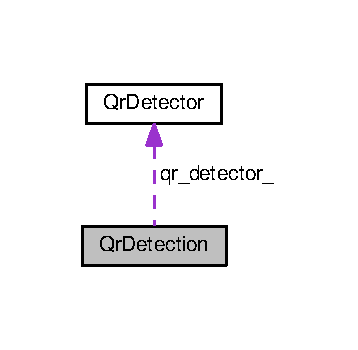
\includegraphics[width=172pt]{classQrDetection__coll__graph}
\end{center}
\end{figure}
\subsection*{Public Member Functions}
\begin{DoxyCompactItemize}
\item 
\hyperlink{classQrDetection_a97890b1548487ff8660924821a7e0e1f}{Qr\-Detection} (void)
\begin{DoxyCompactList}\small\item\em Default constructor. \end{DoxyCompactList}\item 
bool \hyperlink{classQrDetection_a9e81b97a3acc36caa03c2241d649704b}{qr\-Detection\-Callback} (rapp\-\_\-platform\-\_\-ros\-\_\-communications\-::\-Qr\-Detection\-Ros\-Srv\-::\-Request \&req, rapp\-\_\-platform\-\_\-ros\-\_\-communications\-::\-Qr\-Detection\-Ros\-Srv\-::\-Response \&res)
\begin{DoxyCompactList}\small\item\em The qr detection R\-O\-S service callback. \end{DoxyCompactList}\end{DoxyCompactItemize}
\subsection*{Private Attributes}
\begin{DoxyCompactItemize}
\item 
ros\-::\-Node\-Handle \hyperlink{classQrDetection_ab99255e948da428610958e3da45cc692}{nh\-\_\-}
\item 
\hyperlink{classQrDetector}{Qr\-Detector} \hyperlink{classQrDetection_a5417be9d21d01ff82067b022bfd613fe}{qr\-\_\-detector\-\_\-}
\item 
ros\-::\-Service\-Server \hyperlink{classQrDetection_a9785dc6824ccc757d5ba8c22d478b271}{qr\-Detection\-Service\-\_\-}
\item 
std\-::string \hyperlink{classQrDetection_acbf716f43bb9af5cb95cd0289f07269d}{qr\-Detection\-Topic\-\_\-}
\end{DoxyCompactItemize}


\subsection{Detailed Description}
Uptakes the task of setting up the R\-O\-S service callbacks towards qr detection. 

Definition at line 31 of file qr\-\_\-detection.\-h.



\subsection{Constructor \& Destructor Documentation}
\hypertarget{classQrDetection_a97890b1548487ff8660924821a7e0e1f}{\index{Qr\-Detection@{Qr\-Detection}!Qr\-Detection@{Qr\-Detection}}
\index{Qr\-Detection@{Qr\-Detection}!QrDetection@{Qr\-Detection}}
\subsubsection[{Qr\-Detection}]{\setlength{\rightskip}{0pt plus 5cm}Qr\-Detection\-::\-Qr\-Detection (
\begin{DoxyParamCaption}
\item[{void}]{}
\end{DoxyParamCaption}
)}}\label{classQrDetection_a97890b1548487ff8660924821a7e0e1f}


Default constructor. 



Definition at line 23 of file qr\-\_\-detection.\-cpp.



\subsection{Member Function Documentation}
\hypertarget{classQrDetection_a9e81b97a3acc36caa03c2241d649704b}{\index{Qr\-Detection@{Qr\-Detection}!qr\-Detection\-Callback@{qr\-Detection\-Callback}}
\index{qr\-Detection\-Callback@{qr\-Detection\-Callback}!QrDetection@{Qr\-Detection}}
\subsubsection[{qr\-Detection\-Callback}]{\setlength{\rightskip}{0pt plus 5cm}bool Qr\-Detection\-::qr\-Detection\-Callback (
\begin{DoxyParamCaption}
\item[{rapp\-\_\-platform\-\_\-ros\-\_\-communications\-::\-Qr\-Detection\-Ros\-Srv\-::\-Request \&}]{req, }
\item[{rapp\-\_\-platform\-\_\-ros\-\_\-communications\-::\-Qr\-Detection\-Ros\-Srv\-::\-Response \&}]{res}
\end{DoxyParamCaption}
)}}\label{classQrDetection_a9e81b97a3acc36caa03c2241d649704b}


The qr detection R\-O\-S service callback. 


\begin{DoxyParams}{Parameters}
{\em req} & \mbox{[}rapp\-\_\-platform\-\_\-ros\-\_\-communications\-::\-Qr\-Detection\-Ros\-Srv\-::\-Request\&\mbox{]} The service request \\
\hline
{\em res} & \mbox{[}rapp\-\_\-platform\-\_\-ros\-\_\-communications\-::\-Qr\-Detection\-Ros\-Srv\-::\-Response\&\mbox{]} The service response \\
\hline
\end{DoxyParams}
\begin{DoxyReturn}{Returns}
bool -\/ The success status of the call 
\end{DoxyReturn}


Definition at line 40 of file qr\-\_\-detection.\-cpp.



\subsection{Member Data Documentation}
\hypertarget{classQrDetection_ab99255e948da428610958e3da45cc692}{\index{Qr\-Detection@{Qr\-Detection}!nh\-\_\-@{nh\-\_\-}}
\index{nh\-\_\-@{nh\-\_\-}!QrDetection@{Qr\-Detection}}
\subsubsection[{nh\-\_\-}]{\setlength{\rightskip}{0pt plus 5cm}ros\-::\-Node\-Handle Qr\-Detection\-::nh\-\_\-\hspace{0.3cm}{\ttfamily [private]}}}\label{classQrDetection_ab99255e948da428610958e3da45cc692}
$<$ The R\-O\-S node handle The service server 

Definition at line 53 of file qr\-\_\-detection.\-h.

\hypertarget{classQrDetection_a5417be9d21d01ff82067b022bfd613fe}{\index{Qr\-Detection@{Qr\-Detection}!qr\-\_\-detector\-\_\-@{qr\-\_\-detector\-\_\-}}
\index{qr\-\_\-detector\-\_\-@{qr\-\_\-detector\-\_\-}!QrDetection@{Qr\-Detection}}
\subsubsection[{qr\-\_\-detector\-\_\-}]{\setlength{\rightskip}{0pt plus 5cm}{\bf Qr\-Detector} Qr\-Detection\-::qr\-\_\-detector\-\_\-\hspace{0.3cm}{\ttfamily [private]}}}\label{classQrDetection_a5417be9d21d01ff82067b022bfd613fe}


Definition at line 62 of file qr\-\_\-detection.\-h.

\hypertarget{classQrDetection_a9785dc6824ccc757d5ba8c22d478b271}{\index{Qr\-Detection@{Qr\-Detection}!qr\-Detection\-Service\-\_\-@{qr\-Detection\-Service\-\_\-}}
\index{qr\-Detection\-Service\-\_\-@{qr\-Detection\-Service\-\_\-}!QrDetection@{Qr\-Detection}}
\subsubsection[{qr\-Detection\-Service\-\_\-}]{\setlength{\rightskip}{0pt plus 5cm}ros\-::\-Service\-Server Qr\-Detection\-::qr\-Detection\-Service\-\_\-\hspace{0.3cm}{\ttfamily [private]}}}\label{classQrDetection_a9785dc6824ccc757d5ba8c22d478b271}
Topic nomeclarure. Holds the qr detection R\-O\-S service topic U\-R\-I 

Definition at line 56 of file qr\-\_\-detection.\-h.

\hypertarget{classQrDetection_acbf716f43bb9af5cb95cd0289f07269d}{\index{Qr\-Detection@{Qr\-Detection}!qr\-Detection\-Topic\-\_\-@{qr\-Detection\-Topic\-\_\-}}
\index{qr\-Detection\-Topic\-\_\-@{qr\-Detection\-Topic\-\_\-}!QrDetection@{Qr\-Detection}}
\subsubsection[{qr\-Detection\-Topic\-\_\-}]{\setlength{\rightskip}{0pt plus 5cm}std\-::string Qr\-Detection\-::qr\-Detection\-Topic\-\_\-\hspace{0.3cm}{\ttfamily [private]}}}\label{classQrDetection_acbf716f43bb9af5cb95cd0289f07269d}
Object of \hyperlink{classQrDetection}{Qr\-Detection} type 

Definition at line 59 of file qr\-\_\-detection.\-h.



The documentation for this class was generated from the following files\-:\begin{DoxyCompactItemize}
\item 
/home/travis/rapp\-\_\-temp/rapp-\/platform/rapp\-\_\-qr\-\_\-detection/include/qr\-\_\-detection/\hyperlink{qr__detection_8h}{qr\-\_\-detection.\-h}\item 
/home/travis/rapp\-\_\-temp/rapp-\/platform/rapp\-\_\-qr\-\_\-detection/src/\hyperlink{qr__detection_8cpp}{qr\-\_\-detection.\-cpp}\end{DoxyCompactItemize}

\hypertarget{classQrDetector}{\section{Qr\-Detector Class Reference}
\label{classQrDetector}\index{Qr\-Detector@{Qr\-Detector}}
}


Provides the Q\-R detection functionality.  




{\ttfamily \#include $<$qr\-\_\-detector.\-h$>$}

\subsection*{Public Member Functions}
\begin{DoxyCompactItemize}
\item 
\hyperlink{classQrDetector_a467c4d4f36bc4d8ec4f3be3880b57f96}{Qr\-Detector} (void)
\begin{DoxyCompactList}\small\item\em Default constructor. \end{DoxyCompactList}\item 
std\-::vector$<$ \hyperlink{structQrCode}{Qr\-Code} $>$ \hyperlink{classQrDetector_a1f70c86fb01592acb1da2246891e93e2}{detect\-Qrs} (const cv\-::\-Mat \&img)
\begin{DoxyCompactList}\small\item\em Detects Q\-Rs in a cv\-::\-Mat. \end{DoxyCompactList}\item 
std\-::vector$<$ \hyperlink{structQrCode}{Qr\-Code} $>$ \hyperlink{classQrDetector_a2e4bb3be2d9c6a6b7243e9e78402dee9}{find\-Qrs} (std\-::string file\-\_\-name)
\begin{DoxyCompactList}\small\item\em Detects Q\-Rs in an image file. \end{DoxyCompactList}\end{DoxyCompactItemize}
\subsection*{Private Member Functions}
\begin{DoxyCompactItemize}
\item 
cv\-::\-Mat \hyperlink{classQrDetector_a46da54e3da81d4ccc8cee7323237f648}{load\-Image} (std\-::string file\-\_\-name)
\begin{DoxyCompactList}\small\item\em Loads an image into a cv\-::\-Mat structure. \end{DoxyCompactList}\end{DoxyCompactItemize}


\subsection{Detailed Description}
Provides the Q\-R detection functionality. 

Definition at line 45 of file qr\-\_\-detector.\-h.



\subsection{Constructor \& Destructor Documentation}
\hypertarget{classQrDetector_a467c4d4f36bc4d8ec4f3be3880b57f96}{\index{Qr\-Detector@{Qr\-Detector}!Qr\-Detector@{Qr\-Detector}}
\index{Qr\-Detector@{Qr\-Detector}!QrDetector@{Qr\-Detector}}
\subsubsection[{Qr\-Detector}]{\setlength{\rightskip}{0pt plus 5cm}Qr\-Detector\-::\-Qr\-Detector (
\begin{DoxyParamCaption}
\item[{void}]{}
\end{DoxyParamCaption}
)}}\label{classQrDetector_a467c4d4f36bc4d8ec4f3be3880b57f96}


Default constructor. 



Definition at line 23 of file qr\-\_\-detector.\-cpp.



\subsection{Member Function Documentation}
\hypertarget{classQrDetector_a1f70c86fb01592acb1da2246891e93e2}{\index{Qr\-Detector@{Qr\-Detector}!detect\-Qrs@{detect\-Qrs}}
\index{detect\-Qrs@{detect\-Qrs}!QrDetector@{Qr\-Detector}}
\subsubsection[{detect\-Qrs}]{\setlength{\rightskip}{0pt plus 5cm}std\-::vector$<$ {\bf Qr\-Code} $>$ Qr\-Detector\-::detect\-Qrs (
\begin{DoxyParamCaption}
\item[{const cv\-::\-Mat \&}]{input\-\_\-frame}
\end{DoxyParamCaption}
)}}\label{classQrDetector_a1f70c86fb01592acb1da2246891e93e2}


Detects Q\-Rs in a cv\-::\-Mat. 


\begin{DoxyParams}{Parameters}
{\em img} & \mbox{[}const cv\-::\-Mat\&\mbox{]} The input image in cv\-::\-Mat form \\
\hline
\end{DoxyParams}
\begin{DoxyReturn}{Returns}
std\-::vector$<$\-Qr\-Code$>$ The detected Q\-R codes 
\end{DoxyReturn}
$<$ \hyperlink{structQrCode}{Qr\-Code} scanner 

Definition at line 43 of file qr\-\_\-detector.\-cpp.

\hypertarget{classQrDetector_a2e4bb3be2d9c6a6b7243e9e78402dee9}{\index{Qr\-Detector@{Qr\-Detector}!find\-Qrs@{find\-Qrs}}
\index{find\-Qrs@{find\-Qrs}!QrDetector@{Qr\-Detector}}
\subsubsection[{find\-Qrs}]{\setlength{\rightskip}{0pt plus 5cm}std\-::vector$<$ {\bf Qr\-Code} $>$ Qr\-Detector\-::find\-Qrs (
\begin{DoxyParamCaption}
\item[{std\-::string}]{file\-\_\-name}
\end{DoxyParamCaption}
)}}\label{classQrDetector_a2e4bb3be2d9c6a6b7243e9e78402dee9}


Detects Q\-Rs in an image file. 


\begin{DoxyParams}{Parameters}
{\em file\-\_\-name} & \mbox{[}std\-::string\mbox{]} The input image U\-R\-I \\
\hline
\end{DoxyParams}
\begin{DoxyReturn}{Returns}
std\-::vector$<$\-Qr\-Code$>$ The detected Q\-R codes 
\end{DoxyReturn}


Definition at line 101 of file qr\-\_\-detector.\-cpp.

\hypertarget{classQrDetector_a46da54e3da81d4ccc8cee7323237f648}{\index{Qr\-Detector@{Qr\-Detector}!load\-Image@{load\-Image}}
\index{load\-Image@{load\-Image}!QrDetector@{Qr\-Detector}}
\subsubsection[{load\-Image}]{\setlength{\rightskip}{0pt plus 5cm}cv\-::\-Mat Qr\-Detector\-::load\-Image (
\begin{DoxyParamCaption}
\item[{std\-::string}]{file\-\_\-name}
\end{DoxyParamCaption}
)\hspace{0.3cm}{\ttfamily [private]}}}\label{classQrDetector_a46da54e3da81d4ccc8cee7323237f648}


Loads an image into a cv\-::\-Mat structure. 


\begin{DoxyParams}{Parameters}
{\em file\-\_\-name} & \mbox{[}std\-::string\mbox{]} The file U\-R\-I \\
\hline
\end{DoxyParams}
\begin{DoxyReturn}{Returns}
cv\-::\-Mat 
\end{DoxyReturn}


Definition at line 32 of file qr\-\_\-detector.\-cpp.



The documentation for this class was generated from the following files\-:\begin{DoxyCompactItemize}
\item 
/home/travis/rapp\-\_\-temp/rapp-\/platform/rapp\-\_\-qr\-\_\-detection/include/qr\-\_\-detection/\hyperlink{qr__detector_8h}{qr\-\_\-detector.\-h}\item 
/home/travis/rapp\-\_\-temp/rapp-\/platform/rapp\-\_\-qr\-\_\-detection/src/\hyperlink{qr__detector_8cpp}{qr\-\_\-detector.\-cpp}\end{DoxyCompactItemize}

\hypertarget{classrapp__exceptions_1_1RappError}{\section{rapp\-\_\-exceptions.\-Rapp\-Error Class Reference}
\label{classrapp__exceptions_1_1RappError}\index{rapp\-\_\-exceptions.\-Rapp\-Error@{rapp\-\_\-exceptions.\-Rapp\-Error}}
}


Inherits Exception and is used to catch only R\-A\-P\-P-\/specific exceptions.  




Inheritance diagram for rapp\-\_\-exceptions.\-Rapp\-Error\-:


Collaboration diagram for rapp\-\_\-exceptions.\-Rapp\-Error\-:
\subsection*{Public Member Functions}
\begin{DoxyCompactItemize}
\item 
def \hyperlink{classrapp__exceptions_1_1RappError_a90a9797c509de106b6726f50866a1aaa}{\-\_\-\-\_\-init\-\_\-\-\_\-}
\item 
def \hyperlink{classrapp__exceptions_1_1RappError_a90a9797c509de106b6726f50866a1aaa}{\-\_\-\-\_\-init\-\_\-\-\_\-}
\begin{DoxyCompactList}\small\item\em Default contructor. \end{DoxyCompactList}\item 
def \hyperlink{classrapp__exceptions_1_1RappError_aa91e207de1a5fba4ebaf1d4acb0d5951}{\-\_\-\-\_\-str\-\_\-\-\_\-}
\item 
def \hyperlink{classrapp__exceptions_1_1RappError_aa91e207de1a5fba4ebaf1d4acb0d5951}{\-\_\-\-\_\-str\-\_\-\-\_\-}
\begin{DoxyCompactList}\small\item\em Returns the error in a string form. \end{DoxyCompactList}\end{DoxyCompactItemize}
\subsection*{Public Attributes}
\begin{DoxyCompactItemize}
\item 
\hyperlink{classrapp__exceptions_1_1RappError_a4013bcf7e5d7231460c7715a6af02eef}{value}
\end{DoxyCompactItemize}


\subsection{Detailed Description}
Inherits Exception and is used to catch only R\-A\-P\-P-\/specific exceptions. 

\begin{DoxyVerb}Error handling in RAPP\end{DoxyVerb}
 

Definition at line 21 of file rapp\-\_\-exceptions.\-py.



\subsection{Constructor \& Destructor Documentation}
\hypertarget{classrapp__exceptions_1_1RappError_a90a9797c509de106b6726f50866a1aaa}{\index{rapp\-\_\-exceptions\-::\-Rapp\-Error@{rapp\-\_\-exceptions\-::\-Rapp\-Error}!\-\_\-\-\_\-init\-\_\-\-\_\-@{\-\_\-\-\_\-init\-\_\-\-\_\-}}
\index{\-\_\-\-\_\-init\-\_\-\-\_\-@{\-\_\-\-\_\-init\-\_\-\-\_\-}!rapp_exceptions::RappError@{rapp\-\_\-exceptions\-::\-Rapp\-Error}}
\subsubsection[{\-\_\-\-\_\-init\-\_\-\-\_\-}]{\setlength{\rightskip}{0pt plus 5cm}def rapp\-\_\-exceptions.\-Rapp\-Error.\-\_\-\-\_\-init\-\_\-\-\_\- (
\begin{DoxyParamCaption}
\item[{}]{self, }
\item[{}]{value}
\end{DoxyParamCaption}
)}}\label{classrapp__exceptions_1_1RappError_a90a9797c509de106b6726f50866a1aaa}


Default contructor. 



Definition at line 25 of file rapp\-\_\-exceptions.\-py.

\hypertarget{classrapp__exceptions_1_1RappError_a90a9797c509de106b6726f50866a1aaa}{\index{rapp\-\_\-exceptions\-::\-Rapp\-Error@{rapp\-\_\-exceptions\-::\-Rapp\-Error}!\-\_\-\-\_\-init\-\_\-\-\_\-@{\-\_\-\-\_\-init\-\_\-\-\_\-}}
\index{\-\_\-\-\_\-init\-\_\-\-\_\-@{\-\_\-\-\_\-init\-\_\-\-\_\-}!rapp_exceptions::RappError@{rapp\-\_\-exceptions\-::\-Rapp\-Error}}
\subsubsection[{\-\_\-\-\_\-init\-\_\-\-\_\-}]{\setlength{\rightskip}{0pt plus 5cm}def rapp\-\_\-exceptions.\-Rapp\-Error.\-\_\-\-\_\-init\-\_\-\-\_\- (
\begin{DoxyParamCaption}
\item[{}]{self, }
\item[{}]{value}
\end{DoxyParamCaption}
)}}\label{classrapp__exceptions_1_1RappError_a90a9797c509de106b6726f50866a1aaa}


Definition at line 22 of file rapp\-\_\-exceptions.\-py.



\subsection{Member Function Documentation}
\hypertarget{classrapp__exceptions_1_1RappError_aa91e207de1a5fba4ebaf1d4acb0d5951}{\index{rapp\-\_\-exceptions\-::\-Rapp\-Error@{rapp\-\_\-exceptions\-::\-Rapp\-Error}!\-\_\-\-\_\-str\-\_\-\-\_\-@{\-\_\-\-\_\-str\-\_\-\-\_\-}}
\index{\-\_\-\-\_\-str\-\_\-\-\_\-@{\-\_\-\-\_\-str\-\_\-\-\_\-}!rapp_exceptions::RappError@{rapp\-\_\-exceptions\-::\-Rapp\-Error}}
\subsubsection[{\-\_\-\-\_\-str\-\_\-\-\_\-}]{\setlength{\rightskip}{0pt plus 5cm}def rapp\-\_\-exceptions.\-Rapp\-Error.\-\_\-\-\_\-str\-\_\-\-\_\- (
\begin{DoxyParamCaption}
\item[{}]{self}
\end{DoxyParamCaption}
)}}\label{classrapp__exceptions_1_1RappError_aa91e207de1a5fba4ebaf1d4acb0d5951}


Definition at line 25 of file rapp\-\_\-exceptions.\-py.

\hypertarget{classrapp__exceptions_1_1RappError_aa91e207de1a5fba4ebaf1d4acb0d5951}{\index{rapp\-\_\-exceptions\-::\-Rapp\-Error@{rapp\-\_\-exceptions\-::\-Rapp\-Error}!\-\_\-\-\_\-str\-\_\-\-\_\-@{\-\_\-\-\_\-str\-\_\-\-\_\-}}
\index{\-\_\-\-\_\-str\-\_\-\-\_\-@{\-\_\-\-\_\-str\-\_\-\-\_\-}!rapp_exceptions::RappError@{rapp\-\_\-exceptions\-::\-Rapp\-Error}}
\subsubsection[{\-\_\-\-\_\-str\-\_\-\-\_\-}]{\setlength{\rightskip}{0pt plus 5cm}def rapp\-\_\-exceptions.\-Rapp\-Error.\-\_\-\-\_\-str\-\_\-\-\_\- (
\begin{DoxyParamCaption}
\item[{}]{self}
\end{DoxyParamCaption}
)}}\label{classrapp__exceptions_1_1RappError_aa91e207de1a5fba4ebaf1d4acb0d5951}


Returns the error in a string form. 



Definition at line 29 of file rapp\-\_\-exceptions.\-py.



\subsection{Member Data Documentation}
\hypertarget{classrapp__exceptions_1_1RappError_a4013bcf7e5d7231460c7715a6af02eef}{\index{rapp\-\_\-exceptions\-::\-Rapp\-Error@{rapp\-\_\-exceptions\-::\-Rapp\-Error}!value@{value}}
\index{value@{value}!rapp_exceptions::RappError@{rapp\-\_\-exceptions\-::\-Rapp\-Error}}
\subsubsection[{value}]{\setlength{\rightskip}{0pt plus 5cm}rapp\-\_\-exceptions.\-Rapp\-Error.\-value}}\label{classrapp__exceptions_1_1RappError_a4013bcf7e5d7231460c7715a6af02eef}


Definition at line 26 of file rapp\-\_\-exceptions.\-py.



The documentation for this class was generated from the following file\-:\begin{DoxyCompactItemize}
\item 
/home/travis/rapp\-\_\-temp/rapp-\/platform/rapp\-\_\-speech\-\_\-detection\-\_\-google/src/\hyperlink{rapp__speech__detection__google_2src_2rapp__exceptions_8py}{rapp\-\_\-exceptions.\-py}\end{DoxyCompactItemize}

\hypertarget{classrapp__speech__detection__sphinx4_1_1rapp__exceptions_1_1RappError}{\section{rapp\-\_\-speech\-\_\-detection\-\_\-sphinx4.\-rapp\-\_\-exceptions.\-Rapp\-Error Class Reference}
\label{classrapp__speech__detection__sphinx4_1_1rapp__exceptions_1_1RappError}\index{rapp\-\_\-speech\-\_\-detection\-\_\-sphinx4.\-rapp\-\_\-exceptions.\-Rapp\-Error@{rapp\-\_\-speech\-\_\-detection\-\_\-sphinx4.\-rapp\-\_\-exceptions.\-Rapp\-Error}}
}


Provides a R\-A\-P\-P specific exception.  




Inheritance diagram for rapp\-\_\-speech\-\_\-detection\-\_\-sphinx4.\-rapp\-\_\-exceptions.\-Rapp\-Error\-:


Collaboration diagram for rapp\-\_\-speech\-\_\-detection\-\_\-sphinx4.\-rapp\-\_\-exceptions.\-Rapp\-Error\-:
\subsection*{Public Member Functions}
\begin{DoxyCompactItemize}
\item 
def \hyperlink{classrapp__speech__detection__sphinx4_1_1rapp__exceptions_1_1RappError_a96920fb0892c1070dc41c2d19a4d7535}{\-\_\-\-\_\-init\-\_\-\-\_\-}
\item 
def \hyperlink{classrapp__speech__detection__sphinx4_1_1rapp__exceptions_1_1RappError_aebed65d2df9d94ed1bd8f5c30b86a469}{\-\_\-\-\_\-str\-\_\-\-\_\-}
\end{DoxyCompactItemize}
\subsection*{Public Attributes}
\begin{DoxyCompactItemize}
\item 
\hyperlink{classrapp__speech__detection__sphinx4_1_1rapp__exceptions_1_1RappError_a2315c4cb6ee5f5681844294e1ac4c544}{value}
\end{DoxyCompactItemize}


\subsection{Detailed Description}
Provides a R\-A\-P\-P specific exception. 

\begin{DoxyVerb}Error handling in RAPP\end{DoxyVerb}
 

Definition at line 21 of file rapp\-\_\-exceptions.\-py.



\subsection{Constructor \& Destructor Documentation}
\hypertarget{classrapp__speech__detection__sphinx4_1_1rapp__exceptions_1_1RappError_a96920fb0892c1070dc41c2d19a4d7535}{\index{rapp\-\_\-speech\-\_\-detection\-\_\-sphinx4\-::rapp\-\_\-exceptions\-::\-Rapp\-Error@{rapp\-\_\-speech\-\_\-detection\-\_\-sphinx4\-::rapp\-\_\-exceptions\-::\-Rapp\-Error}!\-\_\-\-\_\-init\-\_\-\-\_\-@{\-\_\-\-\_\-init\-\_\-\-\_\-}}
\index{\-\_\-\-\_\-init\-\_\-\-\_\-@{\-\_\-\-\_\-init\-\_\-\-\_\-}!rapp_speech_detection_sphinx4::rapp_exceptions::RappError@{rapp\-\_\-speech\-\_\-detection\-\_\-sphinx4\-::rapp\-\_\-exceptions\-::\-Rapp\-Error}}
\subsubsection[{\-\_\-\-\_\-init\-\_\-\-\_\-}]{\setlength{\rightskip}{0pt plus 5cm}def rapp\-\_\-speech\-\_\-detection\-\_\-sphinx4.\-rapp\-\_\-exceptions.\-Rapp\-Error.\-\_\-\-\_\-init\-\_\-\-\_\- (
\begin{DoxyParamCaption}
\item[{}]{self, }
\item[{}]{value}
\end{DoxyParamCaption}
)}}\label{classrapp__speech__detection__sphinx4_1_1rapp__exceptions_1_1RappError_a96920fb0892c1070dc41c2d19a4d7535}


Definition at line 24 of file rapp\-\_\-exceptions.\-py.



\subsection{Member Function Documentation}
\hypertarget{classrapp__speech__detection__sphinx4_1_1rapp__exceptions_1_1RappError_aebed65d2df9d94ed1bd8f5c30b86a469}{\index{rapp\-\_\-speech\-\_\-detection\-\_\-sphinx4\-::rapp\-\_\-exceptions\-::\-Rapp\-Error@{rapp\-\_\-speech\-\_\-detection\-\_\-sphinx4\-::rapp\-\_\-exceptions\-::\-Rapp\-Error}!\-\_\-\-\_\-str\-\_\-\-\_\-@{\-\_\-\-\_\-str\-\_\-\-\_\-}}
\index{\-\_\-\-\_\-str\-\_\-\-\_\-@{\-\_\-\-\_\-str\-\_\-\-\_\-}!rapp_speech_detection_sphinx4::rapp_exceptions::RappError@{rapp\-\_\-speech\-\_\-detection\-\_\-sphinx4\-::rapp\-\_\-exceptions\-::\-Rapp\-Error}}
\subsubsection[{\-\_\-\-\_\-str\-\_\-\-\_\-}]{\setlength{\rightskip}{0pt plus 5cm}def rapp\-\_\-speech\-\_\-detection\-\_\-sphinx4.\-rapp\-\_\-exceptions.\-Rapp\-Error.\-\_\-\-\_\-str\-\_\-\-\_\- (
\begin{DoxyParamCaption}
\item[{}]{self}
\end{DoxyParamCaption}
)}}\label{classrapp__speech__detection__sphinx4_1_1rapp__exceptions_1_1RappError_aebed65d2df9d94ed1bd8f5c30b86a469}


Definition at line 27 of file rapp\-\_\-exceptions.\-py.



\subsection{Member Data Documentation}
\hypertarget{classrapp__speech__detection__sphinx4_1_1rapp__exceptions_1_1RappError_a2315c4cb6ee5f5681844294e1ac4c544}{\index{rapp\-\_\-speech\-\_\-detection\-\_\-sphinx4\-::rapp\-\_\-exceptions\-::\-Rapp\-Error@{rapp\-\_\-speech\-\_\-detection\-\_\-sphinx4\-::rapp\-\_\-exceptions\-::\-Rapp\-Error}!value@{value}}
\index{value@{value}!rapp_speech_detection_sphinx4::rapp_exceptions::RappError@{rapp\-\_\-speech\-\_\-detection\-\_\-sphinx4\-::rapp\-\_\-exceptions\-::\-Rapp\-Error}}
\subsubsection[{value}]{\setlength{\rightskip}{0pt plus 5cm}rapp\-\_\-speech\-\_\-detection\-\_\-sphinx4.\-rapp\-\_\-exceptions.\-Rapp\-Error.\-value}}\label{classrapp__speech__detection__sphinx4_1_1rapp__exceptions_1_1RappError_a2315c4cb6ee5f5681844294e1ac4c544}


Definition at line 25 of file rapp\-\_\-exceptions.\-py.



The documentation for this class was generated from the following file\-:\begin{DoxyCompactItemize}
\item 
/home/travis/rapp\-\_\-temp/rapp-\/platform/rapp\-\_\-speech\-\_\-detection\-\_\-sphinx4/src/rapp\-\_\-speech\-\_\-detection\-\_\-sphinx4/\hyperlink{rapp__speech__detection__sphinx4_2src_2rapp__speech__detection__sphinx4_2rapp__exceptions_8py}{rapp\-\_\-exceptions.\-py}\end{DoxyCompactItemize}

\hypertarget{classrapp__audio__processing_1_1rapp__set__noise__profile_1_1SetNoiseProfile}{\section{rapp\-\_\-audio\-\_\-processing.\-rapp\-\_\-set\-\_\-noise\-\_\-profile.\-Set\-Noise\-Profile Class Reference}
\label{classrapp__audio__processing_1_1rapp__set__noise__profile_1_1SetNoiseProfile}\index{rapp\-\_\-audio\-\_\-processing.\-rapp\-\_\-set\-\_\-noise\-\_\-profile.\-Set\-Noise\-Profile@{rapp\-\_\-audio\-\_\-processing.\-rapp\-\_\-set\-\_\-noise\-\_\-profile.\-Set\-Noise\-Profile}}
}


Evaluates the noise profile for an audio file.  


\subsection*{Public Member Functions}
\begin{DoxyCompactItemize}
\item 
def \hyperlink{classrapp__audio__processing_1_1rapp__set__noise__profile_1_1SetNoiseProfile_aa8ea75d002c23835ffab8c06d5bedac6}{\-\_\-\-\_\-init\-\_\-\-\_\-}
\begin{DoxyCompactList}\small\item\em Performs initializations. \end{DoxyCompactList}\item 
def \hyperlink{classrapp__audio__processing_1_1rapp__set__noise__profile_1_1SetNoiseProfile_ac66a8db5bcb329d44845fa9703a8e547}{set\-Noise\-\_\-profile}
\begin{DoxyCompactList}\small\item\em Evaluates the audio profile. \end{DoxyCompactList}\end{DoxyCompactItemize}
\subsection*{Public Attributes}
\begin{DoxyCompactItemize}
\item 
\hyperlink{classrapp__audio__processing_1_1rapp__set__noise__profile_1_1SetNoiseProfile_a92b867917dda2074b371fe9bb225df73}{utilities}
\end{DoxyCompactItemize}


\subsection{Detailed Description}
Evaluates the noise profile for an audio file. 

Definition at line 31 of file rapp\-\_\-set\-\_\-noise\-\_\-profile.\-py.



\subsection{Constructor \& Destructor Documentation}
\hypertarget{classrapp__audio__processing_1_1rapp__set__noise__profile_1_1SetNoiseProfile_aa8ea75d002c23835ffab8c06d5bedac6}{\index{rapp\-\_\-audio\-\_\-processing\-::rapp\-\_\-set\-\_\-noise\-\_\-profile\-::\-Set\-Noise\-Profile@{rapp\-\_\-audio\-\_\-processing\-::rapp\-\_\-set\-\_\-noise\-\_\-profile\-::\-Set\-Noise\-Profile}!\-\_\-\-\_\-init\-\_\-\-\_\-@{\-\_\-\-\_\-init\-\_\-\-\_\-}}
\index{\-\_\-\-\_\-init\-\_\-\-\_\-@{\-\_\-\-\_\-init\-\_\-\-\_\-}!rapp_audio_processing::rapp_set_noise_profile::SetNoiseProfile@{rapp\-\_\-audio\-\_\-processing\-::rapp\-\_\-set\-\_\-noise\-\_\-profile\-::\-Set\-Noise\-Profile}}
\subsubsection[{\-\_\-\-\_\-init\-\_\-\-\_\-}]{\setlength{\rightskip}{0pt plus 5cm}def rapp\-\_\-audio\-\_\-processing.\-rapp\-\_\-set\-\_\-noise\-\_\-profile.\-Set\-Noise\-Profile.\-\_\-\-\_\-init\-\_\-\-\_\- (
\begin{DoxyParamCaption}
\item[{}]{self}
\end{DoxyParamCaption}
)}}\label{classrapp__audio__processing_1_1rapp__set__noise__profile_1_1SetNoiseProfile_aa8ea75d002c23835ffab8c06d5bedac6}


Performs initializations. 



Definition at line 34 of file rapp\-\_\-set\-\_\-noise\-\_\-profile.\-py.



\subsection{Member Function Documentation}
\hypertarget{classrapp__audio__processing_1_1rapp__set__noise__profile_1_1SetNoiseProfile_ac66a8db5bcb329d44845fa9703a8e547}{\index{rapp\-\_\-audio\-\_\-processing\-::rapp\-\_\-set\-\_\-noise\-\_\-profile\-::\-Set\-Noise\-Profile@{rapp\-\_\-audio\-\_\-processing\-::rapp\-\_\-set\-\_\-noise\-\_\-profile\-::\-Set\-Noise\-Profile}!set\-Noise\-\_\-profile@{set\-Noise\-\_\-profile}}
\index{set\-Noise\-\_\-profile@{set\-Noise\-\_\-profile}!rapp_audio_processing::rapp_set_noise_profile::SetNoiseProfile@{rapp\-\_\-audio\-\_\-processing\-::rapp\-\_\-set\-\_\-noise\-\_\-profile\-::\-Set\-Noise\-Profile}}
\subsubsection[{set\-Noise\-\_\-profile}]{\setlength{\rightskip}{0pt plus 5cm}def rapp\-\_\-audio\-\_\-processing.\-rapp\-\_\-set\-\_\-noise\-\_\-profile.\-Set\-Noise\-Profile.\-set\-Noise\-\_\-profile (
\begin{DoxyParamCaption}
\item[{}]{self, }
\item[{}]{user, }
\item[{}]{noise\-\_\-audio\-\_\-file, }
\item[{}]{audio\-\_\-file\-\_\-type}
\end{DoxyParamCaption}
)}}\label{classrapp__audio__processing_1_1rapp__set__noise__profile_1_1SetNoiseProfile_ac66a8db5bcb329d44845fa9703a8e547}


Evaluates the audio profile. 

Handles service callback \hyperlink{classrapp__audio__processing_1_1rapp__audio__processing_1_1AudioProcessing_abae3b74a23c3bb6c7d41b31276dfc3cc}{rapp\-\_\-audio\-\_\-processing.\-Audio\-Processing\-::set\-Noise\-Profile\-Callback}


\begin{DoxyParams}{Parameters}
{\em user} & \mbox{[}string\mbox{]} The system user, for environmental variable access \\
\hline
{\em noise\-\_\-audio\-\_\-file} & \mbox{[}string\mbox{]} Noise audio file path \\
\hline
{\em audio\-\_\-type} & \mbox{[}string\mbox{]} Noise audio file's type \\
\hline
\end{DoxyParams}


Definition at line 45 of file rapp\-\_\-set\-\_\-noise\-\_\-profile.\-py.



\subsection{Member Data Documentation}
\hypertarget{classrapp__audio__processing_1_1rapp__set__noise__profile_1_1SetNoiseProfile_a92b867917dda2074b371fe9bb225df73}{\index{rapp\-\_\-audio\-\_\-processing\-::rapp\-\_\-set\-\_\-noise\-\_\-profile\-::\-Set\-Noise\-Profile@{rapp\-\_\-audio\-\_\-processing\-::rapp\-\_\-set\-\_\-noise\-\_\-profile\-::\-Set\-Noise\-Profile}!utilities@{utilities}}
\index{utilities@{utilities}!rapp_audio_processing::rapp_set_noise_profile::SetNoiseProfile@{rapp\-\_\-audio\-\_\-processing\-::rapp\-\_\-set\-\_\-noise\-\_\-profile\-::\-Set\-Noise\-Profile}}
\subsubsection[{utilities}]{\setlength{\rightskip}{0pt plus 5cm}rapp\-\_\-audio\-\_\-processing.\-rapp\-\_\-set\-\_\-noise\-\_\-profile.\-Set\-Noise\-Profile.\-utilities}}\label{classrapp__audio__processing_1_1rapp__set__noise__profile_1_1SetNoiseProfile_a92b867917dda2074b371fe9bb225df73}


Definition at line 35 of file rapp\-\_\-set\-\_\-noise\-\_\-profile.\-py.



The documentation for this class was generated from the following file\-:\begin{DoxyCompactItemize}
\item 
/home/travis/rapp\-\_\-temp/rapp-\/platform/rapp\-\_\-audio\-\_\-processing/src/rapp\-\_\-audio\-\_\-processing/\hyperlink{rapp__set__noise__profile_8py}{rapp\-\_\-set\-\_\-noise\-\_\-profile.\-py}\end{DoxyCompactItemize}

\hypertarget{classrapp__audio__processing_1_1rapp__sox__denoise_1_1SoxDenoise}{\section{rapp\-\_\-audio\-\_\-processing.\-rapp\-\_\-sox\-\_\-denoise.\-Sox\-Denoise Class Reference}
\label{classrapp__audio__processing_1_1rapp__sox__denoise_1_1SoxDenoise}\index{rapp\-\_\-audio\-\_\-processing.\-rapp\-\_\-sox\-\_\-denoise.\-Sox\-Denoise@{rapp\-\_\-audio\-\_\-processing.\-rapp\-\_\-sox\-\_\-denoise.\-Sox\-Denoise}}
}


Performs denoising on an audio file employing Sox application.  


\subsection*{Public Member Functions}
\begin{DoxyCompactItemize}
\item 
def \hyperlink{classrapp__audio__processing_1_1rapp__sox__denoise_1_1SoxDenoise_a96c7e0f872235ce4c383ed775b088a9c}{sox\-Denoise}
\begin{DoxyCompactList}\small\item\em Performs denoising employing Sox apllication. \end{DoxyCompactList}\end{DoxyCompactItemize}


\subsection{Detailed Description}
Performs denoising on an audio file employing Sox application. 

Definition at line 29 of file rapp\-\_\-sox\-\_\-denoise.\-py.



\subsection{Member Function Documentation}
\hypertarget{classrapp__audio__processing_1_1rapp__sox__denoise_1_1SoxDenoise_a96c7e0f872235ce4c383ed775b088a9c}{\index{rapp\-\_\-audio\-\_\-processing\-::rapp\-\_\-sox\-\_\-denoise\-::\-Sox\-Denoise@{rapp\-\_\-audio\-\_\-processing\-::rapp\-\_\-sox\-\_\-denoise\-::\-Sox\-Denoise}!sox\-Denoise@{sox\-Denoise}}
\index{sox\-Denoise@{sox\-Denoise}!rapp_audio_processing::rapp_sox_denoise::SoxDenoise@{rapp\-\_\-audio\-\_\-processing\-::rapp\-\_\-sox\-\_\-denoise\-::\-Sox\-Denoise}}
\subsubsection[{sox\-Denoise}]{\setlength{\rightskip}{0pt plus 5cm}def rapp\-\_\-audio\-\_\-processing.\-rapp\-\_\-sox\-\_\-denoise.\-Sox\-Denoise.\-sox\-Denoise (
\begin{DoxyParamCaption}
\item[{}]{self, }
\item[{}]{user, }
\item[{}]{audio\-\_\-type, }
\item[{}]{audio\-\_\-file, }
\item[{}]{denoised\-\_\-audio\-\_\-file, }
\item[{}]{scale}
\end{DoxyParamCaption}
)}}\label{classrapp__audio__processing_1_1rapp__sox__denoise_1_1SoxDenoise_a96c7e0f872235ce4c383ed775b088a9c}


Performs denoising employing Sox apllication. 

Handles service callback \hyperlink{classrapp__audio__processing_1_1rapp__audio__processing_1_1AudioProcessing_a5280d1ae58e00e61b58959b5c51547ef}{rapp\-\_\-audio\-\_\-processing.\-Audio\-Processing\-::denoise\-Callback}


\begin{DoxyParams}{Parameters}
{\em user} & \mbox{[}string\mbox{]} The system user, for environmental variable access \\
\hline
{\em audio\-\_\-file} & \mbox{[}string\mbox{]} Audio file path \\
\hline
{\em audio\-\_\-type} & \mbox{[}string\mbox{]} Audio file's type \\
\hline
{\em denoised\-\_\-audio\-\_\-file} & \mbox{[}string\mbox{]} Path to write denoised audio file \\
\hline
{\em scale} & \mbox{[}float\mbox{]} Energy denoise scale \\
\hline
\end{DoxyParams}


Definition at line 41 of file rapp\-\_\-sox\-\_\-denoise.\-py.



The documentation for this class was generated from the following file\-:\begin{DoxyCompactItemize}
\item 
/home/travis/rapp\-\_\-temp/rapp-\/platform/rapp\-\_\-audio\-\_\-processing/src/rapp\-\_\-audio\-\_\-processing/\hyperlink{rapp__sox__denoise_8py}{rapp\-\_\-sox\-\_\-denoise.\-py}\end{DoxyCompactItemize}

\hypertarget{classrapp__speech__detection__sphinx4_1_1speech__recognition__sphinx4_1_1SpeechRecognitionSphinx4}{\section{rapp\-\_\-speech\-\_\-detection\-\_\-sphinx4.\-speech\-\_\-recognition\-\_\-sphinx4.\-Speech\-Recognition\-Sphinx4 Class Reference}
\label{classrapp__speech__detection__sphinx4_1_1speech__recognition__sphinx4_1_1SpeechRecognitionSphinx4}\index{rapp\-\_\-speech\-\_\-detection\-\_\-sphinx4.\-speech\-\_\-recognition\-\_\-sphinx4.\-Speech\-Recognition\-Sphinx4@{rapp\-\_\-speech\-\_\-detection\-\_\-sphinx4.\-speech\-\_\-recognition\-\_\-sphinx4.\-Speech\-Recognition\-Sphinx4}}
}


Provides a complete Rapp Sphinx Entity.  


\subsection*{Public Member Functions}
\begin{DoxyCompactItemize}
\item 
def \hyperlink{classrapp__speech__detection__sphinx4_1_1speech__recognition__sphinx4_1_1SpeechRecognitionSphinx4_a43476824e9fc3fe7671164796b1332eb}{\-\_\-\-\_\-init\-\_\-\-\_\-}
\begin{DoxyCompactList}\small\item\em Constructor performing initializations. \end{DoxyCompactList}\item 
def \hyperlink{classrapp__speech__detection__sphinx4_1_1speech__recognition__sphinx4_1_1SpeechRecognitionSphinx4_a547725db1410fdb7ba782387d8ca2507}{get\-Configuration\-Hash}
\begin{DoxyCompactList}\small\item\em Requests the configuration's sha1 hash. \end{DoxyCompactList}\item 
def \hyperlink{classrapp__speech__detection__sphinx4_1_1speech__recognition__sphinx4_1_1SpeechRecognitionSphinx4_a60e2286679d5dce9da486c7b6c3b5ad3}{speech\-Recognition\-Batch}
\begin{DoxyCompactList}\small\item\em Performs \hyperlink{classSphinx4}{Sphinx4} configuration and speech recognition. \end{DoxyCompactList}\end{DoxyCompactItemize}
\subsection*{Private Member Functions}
\begin{DoxyCompactItemize}
\item 
def \hyperlink{classrapp__speech__detection__sphinx4_1_1speech__recognition__sphinx4_1_1SpeechRecognitionSphinx4_a0451d1c7c9a308255d5e93f47b0664f2}{\-\_\-configure\-Speech\-Recognition}
\begin{DoxyCompactList}\small\item\em Performs \hyperlink{classSphinx4}{Sphinx4} configuration. \end{DoxyCompactList}\item 
def \hyperlink{classrapp__speech__detection__sphinx4_1_1speech__recognition__sphinx4_1_1SpeechRecognitionSphinx4_a8b10d0955c0592b98e05b1f5f1cad26a}{\-\_\-create\-Preconfiguration}
\begin{DoxyCompactList}\small\item\em Create the requested preconfiguration. \end{DoxyCompactList}\item 
def \hyperlink{classrapp__speech__detection__sphinx4_1_1speech__recognition__sphinx4_1_1SpeechRecognitionSphinx4_a54a006faca9b32d191e3e4863621a83a}{\-\_\-create\-Support\-Configuration}
\begin{DoxyCompactList}\small\item\em Get Sphinx configuration paths from Language Support. \end{DoxyCompactList}\item 
def \hyperlink{classrapp__speech__detection__sphinx4_1_1speech__recognition__sphinx4_1_1SpeechRecognitionSphinx4_a5ceb0deed7c1dfb1d8bb21c2a401fc93}{\-\_\-select\-Language\-Support}
\begin{DoxyCompactList}\small\item\em Choose the language support based on the request language. \end{DoxyCompactList}\item 
def \hyperlink{classrapp__speech__detection__sphinx4_1_1speech__recognition__sphinx4_1_1SpeechRecognitionSphinx4_a5256ab73fc56d7db4f6e55b36774fa44}{\-\_\-speech\-Recognition}
\begin{DoxyCompactList}\small\item\em Performs \hyperlink{classSphinx4}{Sphinx4} speech recognition. \end{DoxyCompactList}\end{DoxyCompactItemize}
\subsection*{Private Attributes}
\begin{DoxyCompactItemize}
\item 
\hyperlink{classrapp__speech__detection__sphinx4_1_1speech__recognition__sphinx4_1_1SpeechRecognitionSphinx4_ab6a1a99c38bcc6938c0f0a39dd355a04}{\-\_\-configuration\-\_\-params}
\begin{DoxyCompactList}\small\item\em The Sphinx configuration parameters. \end{DoxyCompactList}\item 
\hyperlink{classrapp__speech__detection__sphinx4_1_1speech__recognition__sphinx4_1_1SpeechRecognitionSphinx4_ad506f14432d9452c85b900d79e03c589}{\-\_\-english\-\_\-support}
\begin{DoxyCompactList}\small\item\em English creates necessary files for english speech recognition. \end{DoxyCompactList}\item 
\hyperlink{classrapp__speech__detection__sphinx4_1_1speech__recognition__sphinx4_1_1SpeechRecognitionSphinx4_a530d829504b888823d2e72dafc3ba36c}{\-\_\-global\-Params}
\begin{DoxyCompactList}\small\item\em Contains global Sphinx parameters. \end{DoxyCompactList}\item 
\hyperlink{classrapp__speech__detection__sphinx4_1_1speech__recognition__sphinx4_1_1SpeechRecognitionSphinx4_a4647fa82a552fe670b70550c5e66a253}{\-\_\-greek\-\_\-support}
\begin{DoxyCompactList}\small\item\em Greek\-\_\-support creates necessary files for Greek speech recognition. \end{DoxyCompactList}\item 
\hyperlink{classrapp__speech__detection__sphinx4_1_1speech__recognition__sphinx4_1_1SpeechRecognitionSphinx4_a01424766fb7384f6d005f4be78725af4}{\-\_\-sphinx4}
\begin{DoxyCompactList}\small\item\em The sphinx wrapper communicates with the actual Sphinx.\-java process. \end{DoxyCompactList}\item 
\hyperlink{classrapp__speech__detection__sphinx4_1_1speech__recognition__sphinx4_1_1SpeechRecognitionSphinx4_a752dac4e406d54c3f27db026dca60334}{\-\_\-word\-\_\-mapping}
\begin{DoxyCompactList}\small\item\em A dictionary to transform the englified greek words to actual greek words. \end{DoxyCompactList}\end{DoxyCompactItemize}


\subsection{Detailed Description}
Provides a complete Rapp Sphinx Entity. 

Maintains a complete Rapp Sphinx Entity for the \hyperlink{classrapp__speech__detection__sphinx4_1_1speech__recognition__sphinx4__handler__node_1_1SpeechRecognitionSphinx4HandlerNode}{speech\-\_\-recognition\-\_\-sphinx4\-\_\-handler\-\_\-node.\-Speech\-Recognition\-Sphinx4\-Handler\-Node} to perform the speech recognition. 

Definition at line 61 of file speech\-\_\-recognition\-\_\-sphinx4.\-py.



\subsection{Constructor \& Destructor Documentation}
\hypertarget{classrapp__speech__detection__sphinx4_1_1speech__recognition__sphinx4_1_1SpeechRecognitionSphinx4_a43476824e9fc3fe7671164796b1332eb}{\index{rapp\-\_\-speech\-\_\-detection\-\_\-sphinx4\-::speech\-\_\-recognition\-\_\-sphinx4\-::\-Speech\-Recognition\-Sphinx4@{rapp\-\_\-speech\-\_\-detection\-\_\-sphinx4\-::speech\-\_\-recognition\-\_\-sphinx4\-::\-Speech\-Recognition\-Sphinx4}!\-\_\-\-\_\-init\-\_\-\-\_\-@{\-\_\-\-\_\-init\-\_\-\-\_\-}}
\index{\-\_\-\-\_\-init\-\_\-\-\_\-@{\-\_\-\-\_\-init\-\_\-\-\_\-}!rapp_speech_detection_sphinx4::speech_recognition_sphinx4::SpeechRecognitionSphinx4@{rapp\-\_\-speech\-\_\-detection\-\_\-sphinx4\-::speech\-\_\-recognition\-\_\-sphinx4\-::\-Speech\-Recognition\-Sphinx4}}
\subsubsection[{\-\_\-\-\_\-init\-\_\-\-\_\-}]{\setlength{\rightskip}{0pt plus 5cm}def rapp\-\_\-speech\-\_\-detection\-\_\-sphinx4.\-speech\-\_\-recognition\-\_\-sphinx4.\-Speech\-Recognition\-Sphinx4.\-\_\-\-\_\-init\-\_\-\-\_\- (
\begin{DoxyParamCaption}
\item[{}]{self, }
\item[{}]{configuration\-Name = {\ttfamily None}}
\end{DoxyParamCaption}
)}}\label{classrapp__speech__detection__sphinx4_1_1speech__recognition__sphinx4_1_1SpeechRecognitionSphinx4_a43476824e9fc3fe7671164796b1332eb}


Constructor performing initializations. 



Definition at line 64 of file speech\-\_\-recognition\-\_\-sphinx4.\-py.



\subsection{Member Function Documentation}
\hypertarget{classrapp__speech__detection__sphinx4_1_1speech__recognition__sphinx4_1_1SpeechRecognitionSphinx4_a0451d1c7c9a308255d5e93f47b0664f2}{\index{rapp\-\_\-speech\-\_\-detection\-\_\-sphinx4\-::speech\-\_\-recognition\-\_\-sphinx4\-::\-Speech\-Recognition\-Sphinx4@{rapp\-\_\-speech\-\_\-detection\-\_\-sphinx4\-::speech\-\_\-recognition\-\_\-sphinx4\-::\-Speech\-Recognition\-Sphinx4}!\-\_\-configure\-Speech\-Recognition@{\-\_\-configure\-Speech\-Recognition}}
\index{\-\_\-configure\-Speech\-Recognition@{\-\_\-configure\-Speech\-Recognition}!rapp_speech_detection_sphinx4::speech_recognition_sphinx4::SpeechRecognitionSphinx4@{rapp\-\_\-speech\-\_\-detection\-\_\-sphinx4\-::speech\-\_\-recognition\-\_\-sphinx4\-::\-Speech\-Recognition\-Sphinx4}}
\subsubsection[{\-\_\-configure\-Speech\-Recognition}]{\setlength{\rightskip}{0pt plus 5cm}def rapp\-\_\-speech\-\_\-detection\-\_\-sphinx4.\-speech\-\_\-recognition\-\_\-sphinx4.\-Speech\-Recognition\-Sphinx4.\-\_\-configure\-Speech\-Recognition (
\begin{DoxyParamCaption}
\item[{}]{self, }
\item[{}]{req}
\end{DoxyParamCaption}
)\hspace{0.3cm}{\ttfamily [private]}}}\label{classrapp__speech__detection__sphinx4_1_1speech__recognition__sphinx4_1_1SpeechRecognitionSphinx4_a0451d1c7c9a308255d5e93f47b0664f2}


Performs \hyperlink{classSphinx4}{Sphinx4} configuration. 


\begin{DoxyParams}{Parameters}
{\em req} & \mbox{[}rapp\-\_\-platform\-\_\-ros\-\_\-communications\-::\-Speech\-Detection\-Sphinx4\-Wrapper\-::\-Speech\-Recognition\-Sphinx4\-Configure\-Srv\-Request\mbox{]} The sphinx configuration request \\
\hline
\end{DoxyParams}
\begin{DoxyReturn}{Returns}
res \mbox{[}rapp\-\_\-platform\-\_\-ros\-\_\-communications\-::\-Speech\-Detection\-Sphinx4\-Wrapper\-::\-Speech\-Recognition\-Sphinx4\-Configure\-Srv\-Request\mbox{]} The sphinx configuration response 
\end{DoxyReturn}


Definition at line 189 of file speech\-\_\-recognition\-\_\-sphinx4.\-py.

\hypertarget{classrapp__speech__detection__sphinx4_1_1speech__recognition__sphinx4_1_1SpeechRecognitionSphinx4_a8b10d0955c0592b98e05b1f5f1cad26a}{\index{rapp\-\_\-speech\-\_\-detection\-\_\-sphinx4\-::speech\-\_\-recognition\-\_\-sphinx4\-::\-Speech\-Recognition\-Sphinx4@{rapp\-\_\-speech\-\_\-detection\-\_\-sphinx4\-::speech\-\_\-recognition\-\_\-sphinx4\-::\-Speech\-Recognition\-Sphinx4}!\-\_\-create\-Preconfiguration@{\-\_\-create\-Preconfiguration}}
\index{\-\_\-create\-Preconfiguration@{\-\_\-create\-Preconfiguration}!rapp_speech_detection_sphinx4::speech_recognition_sphinx4::SpeechRecognitionSphinx4@{rapp\-\_\-speech\-\_\-detection\-\_\-sphinx4\-::speech\-\_\-recognition\-\_\-sphinx4\-::\-Speech\-Recognition\-Sphinx4}}
\subsubsection[{\-\_\-create\-Preconfiguration}]{\setlength{\rightskip}{0pt plus 5cm}def rapp\-\_\-speech\-\_\-detection\-\_\-sphinx4.\-speech\-\_\-recognition\-\_\-sphinx4.\-Speech\-Recognition\-Sphinx4.\-\_\-create\-Preconfiguration (
\begin{DoxyParamCaption}
\item[{}]{self, }
\item[{}]{configuration\-Name}
\end{DoxyParamCaption}
)\hspace{0.3cm}{\ttfamily [private]}}}\label{classrapp__speech__detection__sphinx4_1_1speech__recognition__sphinx4_1_1SpeechRecognitionSphinx4_a8b10d0955c0592b98e05b1f5f1cad26a}


Create the requested preconfiguration. 

Creates the configuration via the name requested from rapp\-\_\-speech\-\_\-detection\-\_\-sphinx4\-::cfg\-::sphinx4\-\_\-wrapper\-\_\-params.\-yaml


\begin{DoxyParams}{Parameters}
{\em configuration\-Name} & \mbox{[}string\mbox{]} The preconfiguration name \\
\hline
\end{DoxyParams}


Definition at line 112 of file speech\-\_\-recognition\-\_\-sphinx4.\-py.

\hypertarget{classrapp__speech__detection__sphinx4_1_1speech__recognition__sphinx4_1_1SpeechRecognitionSphinx4_a54a006faca9b32d191e3e4863621a83a}{\index{rapp\-\_\-speech\-\_\-detection\-\_\-sphinx4\-::speech\-\_\-recognition\-\_\-sphinx4\-::\-Speech\-Recognition\-Sphinx4@{rapp\-\_\-speech\-\_\-detection\-\_\-sphinx4\-::speech\-\_\-recognition\-\_\-sphinx4\-::\-Speech\-Recognition\-Sphinx4}!\-\_\-create\-Support\-Configuration@{\-\_\-create\-Support\-Configuration}}
\index{\-\_\-create\-Support\-Configuration@{\-\_\-create\-Support\-Configuration}!rapp_speech_detection_sphinx4::speech_recognition_sphinx4::SpeechRecognitionSphinx4@{rapp\-\_\-speech\-\_\-detection\-\_\-sphinx4\-::speech\-\_\-recognition\-\_\-sphinx4\-::\-Speech\-Recognition\-Sphinx4}}
\subsubsection[{\-\_\-create\-Support\-Configuration}]{\setlength{\rightskip}{0pt plus 5cm}def rapp\-\_\-speech\-\_\-detection\-\_\-sphinx4.\-speech\-\_\-recognition\-\_\-sphinx4.\-Speech\-Recognition\-Sphinx4.\-\_\-create\-Support\-Configuration (
\begin{DoxyParamCaption}
\item[{}]{self, }
\item[{}]{support, }
\item[{}]{res}
\end{DoxyParamCaption}
)\hspace{0.3cm}{\ttfamily [private]}}}\label{classrapp__speech__detection__sphinx4_1_1speech__recognition__sphinx4_1_1SpeechRecognitionSphinx4_a54a006faca9b32d191e3e4863621a83a}


Get Sphinx configuration paths from Language Support. 


\begin{DoxyParams}{Parameters}
{\em support} & \mbox{[}\hyperlink{classrapp__speech__detection__sphinx4_1_1language__support_1_1LanguageSupport}{language\-\_\-support\-::\-Language\-Support}\mbox{]} A child class of the Language\-Support depending on the requested language \\
\hline
{\em req} & \mbox{[}rapp\-\_\-platform\-\_\-ros\-\_\-communications\-::\-Speech\-Detection\-Sphinx4\-Wrapper\-::\-Speech\-Recognition\-Sphinx4\-Configure\-Srv\-Request\mbox{]} The sphinx configuration request\\
\hline
\end{DoxyParams}
\begin{DoxyReturn}{Returns}
conf \mbox{[}dictionary\mbox{]} The Sphinx configuration files' paths 
\end{DoxyReturn}


Definition at line 229 of file speech\-\_\-recognition\-\_\-sphinx4.\-py.

\hypertarget{classrapp__speech__detection__sphinx4_1_1speech__recognition__sphinx4_1_1SpeechRecognitionSphinx4_a5ceb0deed7c1dfb1d8bb21c2a401fc93}{\index{rapp\-\_\-speech\-\_\-detection\-\_\-sphinx4\-::speech\-\_\-recognition\-\_\-sphinx4\-::\-Speech\-Recognition\-Sphinx4@{rapp\-\_\-speech\-\_\-detection\-\_\-sphinx4\-::speech\-\_\-recognition\-\_\-sphinx4\-::\-Speech\-Recognition\-Sphinx4}!\-\_\-select\-Language\-Support@{\-\_\-select\-Language\-Support}}
\index{\-\_\-select\-Language\-Support@{\-\_\-select\-Language\-Support}!rapp_speech_detection_sphinx4::speech_recognition_sphinx4::SpeechRecognitionSphinx4@{rapp\-\_\-speech\-\_\-detection\-\_\-sphinx4\-::speech\-\_\-recognition\-\_\-sphinx4\-::\-Speech\-Recognition\-Sphinx4}}
\subsubsection[{\-\_\-select\-Language\-Support}]{\setlength{\rightskip}{0pt plus 5cm}def rapp\-\_\-speech\-\_\-detection\-\_\-sphinx4.\-speech\-\_\-recognition\-\_\-sphinx4.\-Speech\-Recognition\-Sphinx4.\-\_\-select\-Language\-Support (
\begin{DoxyParamCaption}
\item[{}]{self, }
\item[{}]{req}
\end{DoxyParamCaption}
)\hspace{0.3cm}{\ttfamily [private]}}}\label{classrapp__speech__detection__sphinx4_1_1speech__recognition__sphinx4_1_1SpeechRecognitionSphinx4_a5ceb0deed7c1dfb1d8bb21c2a401fc93}


Choose the language support based on the request language. 


\begin{DoxyParams}{Parameters}
{\em req} & \mbox{[}rapp\-\_\-platform\-\_\-ros\-\_\-communications\-::\-Speech\-Detection\-Sphinx4\-Wrapper\-::\-Speech\-Recognition\-Sphinx4\-Configure\-Srv\-Request\mbox{]} The sphinx configuration request\\
\hline
\end{DoxyParams}
\begin{DoxyReturn}{Returns}
support \mbox{[}\hyperlink{classrapp__speech__detection__sphinx4_1_1language__support_1_1LanguageSupport}{language\-\_\-support\-::\-Language\-Support}\mbox{]} A child class of the Language\-Support depending on the requested language 
\end{DoxyReturn}


Definition at line 175 of file speech\-\_\-recognition\-\_\-sphinx4.\-py.

\hypertarget{classrapp__speech__detection__sphinx4_1_1speech__recognition__sphinx4_1_1SpeechRecognitionSphinx4_a5256ab73fc56d7db4f6e55b36774fa44}{\index{rapp\-\_\-speech\-\_\-detection\-\_\-sphinx4\-::speech\-\_\-recognition\-\_\-sphinx4\-::\-Speech\-Recognition\-Sphinx4@{rapp\-\_\-speech\-\_\-detection\-\_\-sphinx4\-::speech\-\_\-recognition\-\_\-sphinx4\-::\-Speech\-Recognition\-Sphinx4}!\-\_\-speech\-Recognition@{\-\_\-speech\-Recognition}}
\index{\-\_\-speech\-Recognition@{\-\_\-speech\-Recognition}!rapp_speech_detection_sphinx4::speech_recognition_sphinx4::SpeechRecognitionSphinx4@{rapp\-\_\-speech\-\_\-detection\-\_\-sphinx4\-::speech\-\_\-recognition\-\_\-sphinx4\-::\-Speech\-Recognition\-Sphinx4}}
\subsubsection[{\-\_\-speech\-Recognition}]{\setlength{\rightskip}{0pt plus 5cm}def rapp\-\_\-speech\-\_\-detection\-\_\-sphinx4.\-speech\-\_\-recognition\-\_\-sphinx4.\-Speech\-Recognition\-Sphinx4.\-\_\-speech\-Recognition (
\begin{DoxyParamCaption}
\item[{}]{self, }
\item[{}]{req}
\end{DoxyParamCaption}
)\hspace{0.3cm}{\ttfamily [private]}}}\label{classrapp__speech__detection__sphinx4_1_1speech__recognition__sphinx4_1_1SpeechRecognitionSphinx4_a5256ab73fc56d7db4f6e55b36774fa44}


Performs \hyperlink{classSphinx4}{Sphinx4} speech recognition. 


\begin{DoxyParams}{Parameters}
{\em req} & \mbox{[}rapp\-\_\-platform\-\_\-ros\-\_\-communications\-::\-Speech\-Detection\-Sphinx4\-Wrapper\-::\-Speech\-Recognition\-Sphinx4\-Srv\-Request\mbox{]} The speech recognition request \\
\hline
\end{DoxyParams}
\begin{DoxyReturn}{Returns}
res \mbox{[}rapp\-\_\-platform\-\_\-ros\-\_\-communications\-::\-Speech\-Detection\-Sphinx4\-Wrapper\-::\-Speech\-Recognition\-Sphinx4\-Srv\-Response\mbox{]} The speech recognition response 
\end{DoxyReturn}


Definition at line 152 of file speech\-\_\-recognition\-\_\-sphinx4.\-py.

\hypertarget{classrapp__speech__detection__sphinx4_1_1speech__recognition__sphinx4_1_1SpeechRecognitionSphinx4_a547725db1410fdb7ba782387d8ca2507}{\index{rapp\-\_\-speech\-\_\-detection\-\_\-sphinx4\-::speech\-\_\-recognition\-\_\-sphinx4\-::\-Speech\-Recognition\-Sphinx4@{rapp\-\_\-speech\-\_\-detection\-\_\-sphinx4\-::speech\-\_\-recognition\-\_\-sphinx4\-::\-Speech\-Recognition\-Sphinx4}!get\-Configuration\-Hash@{get\-Configuration\-Hash}}
\index{get\-Configuration\-Hash@{get\-Configuration\-Hash}!rapp_speech_detection_sphinx4::speech_recognition_sphinx4::SpeechRecognitionSphinx4@{rapp\-\_\-speech\-\_\-detection\-\_\-sphinx4\-::speech\-\_\-recognition\-\_\-sphinx4\-::\-Speech\-Recognition\-Sphinx4}}
\subsubsection[{get\-Configuration\-Hash}]{\setlength{\rightskip}{0pt plus 5cm}def rapp\-\_\-speech\-\_\-detection\-\_\-sphinx4.\-speech\-\_\-recognition\-\_\-sphinx4.\-Speech\-Recognition\-Sphinx4.\-get\-Configuration\-Hash (
\begin{DoxyParamCaption}
\item[{}]{self}
\end{DoxyParamCaption}
)}}\label{classrapp__speech__detection__sphinx4_1_1speech__recognition__sphinx4_1_1SpeechRecognitionSphinx4_a547725db1410fdb7ba782387d8ca2507}


Requests the configuration's sha1 hash. 

Hash is used to identify common request configurations for proper subprocess selection. (Requests with common requests do not require reconfiguration reducing computation time)

\begin{DoxyReturn}{Returns}
hexdigest \mbox{[}string\mbox{]} The hash digest containing only hexadecimal digits 
\end{DoxyReturn}


Definition at line 103 of file speech\-\_\-recognition\-\_\-sphinx4.\-py.

\hypertarget{classrapp__speech__detection__sphinx4_1_1speech__recognition__sphinx4_1_1SpeechRecognitionSphinx4_a60e2286679d5dce9da486c7b6c3b5ad3}{\index{rapp\-\_\-speech\-\_\-detection\-\_\-sphinx4\-::speech\-\_\-recognition\-\_\-sphinx4\-::\-Speech\-Recognition\-Sphinx4@{rapp\-\_\-speech\-\_\-detection\-\_\-sphinx4\-::speech\-\_\-recognition\-\_\-sphinx4\-::\-Speech\-Recognition\-Sphinx4}!speech\-Recognition\-Batch@{speech\-Recognition\-Batch}}
\index{speech\-Recognition\-Batch@{speech\-Recognition\-Batch}!rapp_speech_detection_sphinx4::speech_recognition_sphinx4::SpeechRecognitionSphinx4@{rapp\-\_\-speech\-\_\-detection\-\_\-sphinx4\-::speech\-\_\-recognition\-\_\-sphinx4\-::\-Speech\-Recognition\-Sphinx4}}
\subsubsection[{speech\-Recognition\-Batch}]{\setlength{\rightskip}{0pt plus 5cm}def rapp\-\_\-speech\-\_\-detection\-\_\-sphinx4.\-speech\-\_\-recognition\-\_\-sphinx4.\-Speech\-Recognition\-Sphinx4.\-speech\-Recognition\-Batch (
\begin{DoxyParamCaption}
\item[{}]{self, }
\item[{}]{req}
\end{DoxyParamCaption}
)}}\label{classrapp__speech__detection__sphinx4_1_1speech__recognition__sphinx4_1_1SpeechRecognitionSphinx4_a60e2286679d5dce9da486c7b6c3b5ad3}


Performs \hyperlink{classSphinx4}{Sphinx4} configuration and speech recognition. 


\begin{DoxyParams}{Parameters}
{\em req} & \mbox{[}rapp\-\_\-platform\-\_\-ros\-\_\-communications\-::\-Speech\-Detection\-Sphinx4\-Wrapper\-::\-Speech\-Recognition\-Sphinx4\-Total\-Srv\-Request\mbox{]} The speech recognition request \\
\hline
\end{DoxyParams}
\begin{DoxyReturn}{Returns}
res \mbox{[}rapp\-\_\-platform\-\_\-ros\-\_\-communications\-::\-Speech\-Detection\-Sphinx4\-Wrapper\-::\-Speech\-Recognition\-Sphinx4\-Total\-Srv\-Response\mbox{]} The speech recognition response 
\end{DoxyReturn}


Definition at line 128 of file speech\-\_\-recognition\-\_\-sphinx4.\-py.



\subsection{Member Data Documentation}
\hypertarget{classrapp__speech__detection__sphinx4_1_1speech__recognition__sphinx4_1_1SpeechRecognitionSphinx4_ab6a1a99c38bcc6938c0f0a39dd355a04}{\index{rapp\-\_\-speech\-\_\-detection\-\_\-sphinx4\-::speech\-\_\-recognition\-\_\-sphinx4\-::\-Speech\-Recognition\-Sphinx4@{rapp\-\_\-speech\-\_\-detection\-\_\-sphinx4\-::speech\-\_\-recognition\-\_\-sphinx4\-::\-Speech\-Recognition\-Sphinx4}!\-\_\-configuration\-\_\-params@{\-\_\-configuration\-\_\-params}}
\index{\-\_\-configuration\-\_\-params@{\-\_\-configuration\-\_\-params}!rapp_speech_detection_sphinx4::speech_recognition_sphinx4::SpeechRecognitionSphinx4@{rapp\-\_\-speech\-\_\-detection\-\_\-sphinx4\-::speech\-\_\-recognition\-\_\-sphinx4\-::\-Speech\-Recognition\-Sphinx4}}
\subsubsection[{\-\_\-configuration\-\_\-params}]{\setlength{\rightskip}{0pt plus 5cm}rapp\-\_\-speech\-\_\-detection\-\_\-sphinx4.\-speech\-\_\-recognition\-\_\-sphinx4.\-Speech\-Recognition\-Sphinx4.\-\_\-configuration\-\_\-params\hspace{0.3cm}{\ttfamily [private]}}}\label{classrapp__speech__detection__sphinx4_1_1speech__recognition__sphinx4_1_1SpeechRecognitionSphinx4_ab6a1a99c38bcc6938c0f0a39dd355a04}


The Sphinx configuration parameters. 

(see \hyperlink{classrapp__speech__detection__sphinx4_1_1sphinx4__configuration__params_1_1SphinxConfigurationParams}{sphinx4\-\_\-configuration\-\_\-params.\-Sphinx\-Configuration\-Params}) 

Definition at line 86 of file speech\-\_\-recognition\-\_\-sphinx4.\-py.

\hypertarget{classrapp__speech__detection__sphinx4_1_1speech__recognition__sphinx4_1_1SpeechRecognitionSphinx4_ad506f14432d9452c85b900d79e03c589}{\index{rapp\-\_\-speech\-\_\-detection\-\_\-sphinx4\-::speech\-\_\-recognition\-\_\-sphinx4\-::\-Speech\-Recognition\-Sphinx4@{rapp\-\_\-speech\-\_\-detection\-\_\-sphinx4\-::speech\-\_\-recognition\-\_\-sphinx4\-::\-Speech\-Recognition\-Sphinx4}!\-\_\-english\-\_\-support@{\-\_\-english\-\_\-support}}
\index{\-\_\-english\-\_\-support@{\-\_\-english\-\_\-support}!rapp_speech_detection_sphinx4::speech_recognition_sphinx4::SpeechRecognitionSphinx4@{rapp\-\_\-speech\-\_\-detection\-\_\-sphinx4\-::speech\-\_\-recognition\-\_\-sphinx4\-::\-Speech\-Recognition\-Sphinx4}}
\subsubsection[{\-\_\-english\-\_\-support}]{\setlength{\rightskip}{0pt plus 5cm}rapp\-\_\-speech\-\_\-detection\-\_\-sphinx4.\-speech\-\_\-recognition\-\_\-sphinx4.\-Speech\-Recognition\-Sphinx4.\-\_\-english\-\_\-support\hspace{0.3cm}{\ttfamily [private]}}}\label{classrapp__speech__detection__sphinx4_1_1speech__recognition__sphinx4_1_1SpeechRecognitionSphinx4_ad506f14432d9452c85b900d79e03c589}


English creates necessary files for english speech recognition. 

(see \hyperlink{classrapp__speech__detection__sphinx4_1_1english__support_1_1EnglishSupport}{english\-\_\-support.\-English\-Support}) 

Definition at line 82 of file speech\-\_\-recognition\-\_\-sphinx4.\-py.

\hypertarget{classrapp__speech__detection__sphinx4_1_1speech__recognition__sphinx4_1_1SpeechRecognitionSphinx4_a530d829504b888823d2e72dafc3ba36c}{\index{rapp\-\_\-speech\-\_\-detection\-\_\-sphinx4\-::speech\-\_\-recognition\-\_\-sphinx4\-::\-Speech\-Recognition\-Sphinx4@{rapp\-\_\-speech\-\_\-detection\-\_\-sphinx4\-::speech\-\_\-recognition\-\_\-sphinx4\-::\-Speech\-Recognition\-Sphinx4}!\-\_\-global\-Params@{\-\_\-global\-Params}}
\index{\-\_\-global\-Params@{\-\_\-global\-Params}!rapp_speech_detection_sphinx4::speech_recognition_sphinx4::SpeechRecognitionSphinx4@{rapp\-\_\-speech\-\_\-detection\-\_\-sphinx4\-::speech\-\_\-recognition\-\_\-sphinx4\-::\-Speech\-Recognition\-Sphinx4}}
\subsubsection[{\-\_\-global\-Params}]{\setlength{\rightskip}{0pt plus 5cm}rapp\-\_\-speech\-\_\-detection\-\_\-sphinx4.\-speech\-\_\-recognition\-\_\-sphinx4.\-Speech\-Recognition\-Sphinx4.\-\_\-global\-Params\hspace{0.3cm}{\ttfamily [private]}}}\label{classrapp__speech__detection__sphinx4_1_1speech__recognition__sphinx4_1_1SpeechRecognitionSphinx4_a530d829504b888823d2e72dafc3ba36c}


Contains global Sphinx parameters. 

(see \hyperlink{classrapp__speech__detection__sphinx4_1_1global__parameters_1_1GlobalParams}{global\-\_\-parameters.\-Global\-Params}) 

Definition at line 69 of file speech\-\_\-recognition\-\_\-sphinx4.\-py.

\hypertarget{classrapp__speech__detection__sphinx4_1_1speech__recognition__sphinx4_1_1SpeechRecognitionSphinx4_a4647fa82a552fe670b70550c5e66a253}{\index{rapp\-\_\-speech\-\_\-detection\-\_\-sphinx4\-::speech\-\_\-recognition\-\_\-sphinx4\-::\-Speech\-Recognition\-Sphinx4@{rapp\-\_\-speech\-\_\-detection\-\_\-sphinx4\-::speech\-\_\-recognition\-\_\-sphinx4\-::\-Speech\-Recognition\-Sphinx4}!\-\_\-greek\-\_\-support@{\-\_\-greek\-\_\-support}}
\index{\-\_\-greek\-\_\-support@{\-\_\-greek\-\_\-support}!rapp_speech_detection_sphinx4::speech_recognition_sphinx4::SpeechRecognitionSphinx4@{rapp\-\_\-speech\-\_\-detection\-\_\-sphinx4\-::speech\-\_\-recognition\-\_\-sphinx4\-::\-Speech\-Recognition\-Sphinx4}}
\subsubsection[{\-\_\-greek\-\_\-support}]{\setlength{\rightskip}{0pt plus 5cm}rapp\-\_\-speech\-\_\-detection\-\_\-sphinx4.\-speech\-\_\-recognition\-\_\-sphinx4.\-Speech\-Recognition\-Sphinx4.\-\_\-greek\-\_\-support\hspace{0.3cm}{\ttfamily [private]}}}\label{classrapp__speech__detection__sphinx4_1_1speech__recognition__sphinx4_1_1SpeechRecognitionSphinx4_a4647fa82a552fe670b70550c5e66a253}


Greek\-\_\-support creates necessary files for Greek speech recognition. 

(see \hyperlink{classrapp__speech__detection__sphinx4_1_1greek__support_1_1GreekSupport}{greek\-\_\-support.\-Greek\-Support}) 

Definition at line 78 of file speech\-\_\-recognition\-\_\-sphinx4.\-py.

\hypertarget{classrapp__speech__detection__sphinx4_1_1speech__recognition__sphinx4_1_1SpeechRecognitionSphinx4_a01424766fb7384f6d005f4be78725af4}{\index{rapp\-\_\-speech\-\_\-detection\-\_\-sphinx4\-::speech\-\_\-recognition\-\_\-sphinx4\-::\-Speech\-Recognition\-Sphinx4@{rapp\-\_\-speech\-\_\-detection\-\_\-sphinx4\-::speech\-\_\-recognition\-\_\-sphinx4\-::\-Speech\-Recognition\-Sphinx4}!\-\_\-sphinx4@{\-\_\-sphinx4}}
\index{\-\_\-sphinx4@{\-\_\-sphinx4}!rapp_speech_detection_sphinx4::speech_recognition_sphinx4::SpeechRecognitionSphinx4@{rapp\-\_\-speech\-\_\-detection\-\_\-sphinx4\-::speech\-\_\-recognition\-\_\-sphinx4\-::\-Speech\-Recognition\-Sphinx4}}
\subsubsection[{\-\_\-sphinx4}]{\setlength{\rightskip}{0pt plus 5cm}rapp\-\_\-speech\-\_\-detection\-\_\-sphinx4.\-speech\-\_\-recognition\-\_\-sphinx4.\-Speech\-Recognition\-Sphinx4.\-\_\-sphinx4\hspace{0.3cm}{\ttfamily [private]}}}\label{classrapp__speech__detection__sphinx4_1_1speech__recognition__sphinx4_1_1SpeechRecognitionSphinx4_a01424766fb7384f6d005f4be78725af4}


The sphinx wrapper communicates with the actual Sphinx.\-java process. 

(see \hyperlink{classrapp__speech__detection__sphinx4_1_1sphinx4__wrapper_1_1Sphinx4Wrapper}{sphinx4\-\_\-wrapper.\-Sphinx4\-Wrapper}) 

Definition at line 74 of file speech\-\_\-recognition\-\_\-sphinx4.\-py.

\hypertarget{classrapp__speech__detection__sphinx4_1_1speech__recognition__sphinx4_1_1SpeechRecognitionSphinx4_a752dac4e406d54c3f27db026dca60334}{\index{rapp\-\_\-speech\-\_\-detection\-\_\-sphinx4\-::speech\-\_\-recognition\-\_\-sphinx4\-::\-Speech\-Recognition\-Sphinx4@{rapp\-\_\-speech\-\_\-detection\-\_\-sphinx4\-::speech\-\_\-recognition\-\_\-sphinx4\-::\-Speech\-Recognition\-Sphinx4}!\-\_\-word\-\_\-mapping@{\-\_\-word\-\_\-mapping}}
\index{\-\_\-word\-\_\-mapping@{\-\_\-word\-\_\-mapping}!rapp_speech_detection_sphinx4::speech_recognition_sphinx4::SpeechRecognitionSphinx4@{rapp\-\_\-speech\-\_\-detection\-\_\-sphinx4\-::speech\-\_\-recognition\-\_\-sphinx4\-::\-Speech\-Recognition\-Sphinx4}}
\subsubsection[{\-\_\-word\-\_\-mapping}]{\setlength{\rightskip}{0pt plus 5cm}rapp\-\_\-speech\-\_\-detection\-\_\-sphinx4.\-speech\-\_\-recognition\-\_\-sphinx4.\-Speech\-Recognition\-Sphinx4.\-\_\-word\-\_\-mapping\hspace{0.3cm}{\ttfamily [private]}}}\label{classrapp__speech__detection__sphinx4_1_1speech__recognition__sphinx4_1_1SpeechRecognitionSphinx4_a752dac4e406d54c3f27db026dca60334}


A dictionary to transform the englified greek words to actual greek words. 



Definition at line 89 of file speech\-\_\-recognition\-\_\-sphinx4.\-py.



The documentation for this class was generated from the following file\-:\begin{DoxyCompactItemize}
\item 
/home/travis/rapp\-\_\-temp/rapp-\/platform/rapp\-\_\-speech\-\_\-detection\-\_\-sphinx4/src/rapp\-\_\-speech\-\_\-detection\-\_\-sphinx4/\hyperlink{speech__recognition__sphinx4_8py}{speech\-\_\-recognition\-\_\-sphinx4.\-py}\end{DoxyCompactItemize}

\hypertarget{classrapp__speech__detection__sphinx4_1_1speech__recognition__sphinx4__handler__node_1_1SpeechRecognitionSphinx4HandlerNode}{\section{rapp\-\_\-speech\-\_\-detection\-\_\-sphinx4.\-speech\-\_\-recognition\-\_\-sphinx4\-\_\-handler\-\_\-node.\-Speech\-Recognition\-Sphinx4\-Handler\-Node Class Reference}
\label{classrapp__speech__detection__sphinx4_1_1speech__recognition__sphinx4__handler__node_1_1SpeechRecognitionSphinx4HandlerNode}\index{rapp\-\_\-speech\-\_\-detection\-\_\-sphinx4.\-speech\-\_\-recognition\-\_\-sphinx4\-\_\-handler\-\_\-node.\-Speech\-Recognition\-Sphinx4\-Handler\-Node@{rapp\-\_\-speech\-\_\-detection\-\_\-sphinx4.\-speech\-\_\-recognition\-\_\-sphinx4\-\_\-handler\-\_\-node.\-Speech\-Recognition\-Sphinx4\-Handler\-Node}}
}


Maintains Sphinx instances to perform speech recognition.  


\subsection*{Public Member Functions}
\begin{DoxyCompactItemize}
\item 
def \hyperlink{classrapp__speech__detection__sphinx4_1_1speech__recognition__sphinx4__handler__node_1_1SpeechRecognitionSphinx4HandlerNode_a82c15c573f92e81d51b4d07bdf8d801c}{\-\_\-\-\_\-init\-\_\-\-\_\-}
\begin{DoxyCompactList}\small\item\em Initializes the subprocesses and the services (constructor) \end{DoxyCompactList}\item 
def \hyperlink{classrapp__speech__detection__sphinx4_1_1speech__recognition__sphinx4__handler__node_1_1SpeechRecognitionSphinx4HandlerNode_ab2a5e3c1fb1b126c727ac554147830b1}{handle\-Speech\-Recognition\-Callback}
\begin{DoxyCompactList}\small\item\em The callback to perform speech recognition. \end{DoxyCompactList}\end{DoxyCompactItemize}
\subsection*{Private Member Functions}
\begin{DoxyCompactItemize}
\item 
def \hyperlink{classrapp__speech__detection__sphinx4_1_1speech__recognition__sphinx4__handler__node_1_1SpeechRecognitionSphinx4HandlerNode_ab0aee24f2a30e54932d173dbfe4063aa}{\-\_\-calculate\-Request\-Hash}
\begin{DoxyCompactList}\small\item\em Calculates the service request sha1 hash for process handling purposes. \end{DoxyCompactList}\item 
def \hyperlink{classrapp__speech__detection__sphinx4_1_1speech__recognition__sphinx4__handler__node_1_1SpeechRecognitionSphinx4HandlerNode_a0c7361126cde2b0e291506310ac022f5}{\-\_\-get\-Preconfiguration\-Names}
\begin{DoxyCompactList}\small\item\em Specifies the requested preconfiguration names. \end{DoxyCompactList}\end{DoxyCompactItemize}
\subsection*{Private Attributes}
\begin{DoxyCompactItemize}
\item 
\hyperlink{classrapp__speech__detection__sphinx4_1_1speech__recognition__sphinx4__handler__node_1_1SpeechRecognitionSphinx4HandlerNode_a528ab714ddc50a375936f09d62ec2a8a}{\-\_\-available\-Processes}
\begin{DoxyCompactList}\small\item\em The subprocesses structure that contains information used for the subprocess handling. \end{DoxyCompactList}\item 
\hyperlink{classrapp__speech__detection__sphinx4_1_1speech__recognition__sphinx4__handler__node_1_1SpeechRecognitionSphinx4HandlerNode_a26891ed7d1142f5f72cf81c7ff98d8d2}{\-\_\-lock}
\begin{DoxyCompactList}\small\item\em Thread conditional variable used for the subprocess scheduling. \end{DoxyCompactList}\item 
\hyperlink{classrapp__speech__detection__sphinx4_1_1speech__recognition__sphinx4__handler__node_1_1SpeechRecognitionSphinx4HandlerNode_a8ab91d66cd73549bbd374c2ead550323}{\-\_\-speech\-\_\-recognition\-\_\-batch\-\_\-service}
\begin{DoxyCompactList}\small\item\em Ros service server for sphinx speech recognition. \end{DoxyCompactList}\item 
\hyperlink{classrapp__speech__detection__sphinx4_1_1speech__recognition__sphinx4__handler__node_1_1SpeechRecognitionSphinx4HandlerNode_a385903b4de07e56f2d6b341c67497053}{\-\_\-thread\-Counter}
\begin{DoxyCompactList}\small\item\em Total service callback threads waiting to execute. \end{DoxyCompactList}\item 
\hyperlink{classrapp__speech__detection__sphinx4_1_1speech__recognition__sphinx4__handler__node_1_1SpeechRecognitionSphinx4HandlerNode_ab0d95faf8af87481f4d1cc04dca1ff9c}{\-\_\-threads}
\begin{DoxyCompactList}\small\item\em The number of child subprocesses. \end{DoxyCompactList}\end{DoxyCompactItemize}


\subsection{Detailed Description}
Maintains Sphinx instances to perform speech recognition. 

Maintains a number of child processes to perform speech recognition utilizing \hyperlink{classSphinx4}{Sphinx4} (\hyperlink{classrapp__speech__detection__sphinx4_1_1speech__recognition__sphinx4_1_1SpeechRecognitionSphinx4}{rapp\-\_\-speech\-\_\-detection\-\_\-sphinx4.\-speech\-\_\-recognition\-\_\-sphinx4.\-Speech\-Recognition\-Sphinx4}). Provides ros services and handles the requests according to the child processes' status. 

Definition at line 47 of file speech\-\_\-recognition\-\_\-sphinx4\-\_\-handler\-\_\-node.\-py.



\subsection{Constructor \& Destructor Documentation}
\hypertarget{classrapp__speech__detection__sphinx4_1_1speech__recognition__sphinx4__handler__node_1_1SpeechRecognitionSphinx4HandlerNode_a82c15c573f92e81d51b4d07bdf8d801c}{\index{rapp\-\_\-speech\-\_\-detection\-\_\-sphinx4\-::speech\-\_\-recognition\-\_\-sphinx4\-\_\-handler\-\_\-node\-::\-Speech\-Recognition\-Sphinx4\-Handler\-Node@{rapp\-\_\-speech\-\_\-detection\-\_\-sphinx4\-::speech\-\_\-recognition\-\_\-sphinx4\-\_\-handler\-\_\-node\-::\-Speech\-Recognition\-Sphinx4\-Handler\-Node}!\-\_\-\-\_\-init\-\_\-\-\_\-@{\-\_\-\-\_\-init\-\_\-\-\_\-}}
\index{\-\_\-\-\_\-init\-\_\-\-\_\-@{\-\_\-\-\_\-init\-\_\-\-\_\-}!rapp_speech_detection_sphinx4::speech_recognition_sphinx4_handler_node::SpeechRecognitionSphinx4HandlerNode@{rapp\-\_\-speech\-\_\-detection\-\_\-sphinx4\-::speech\-\_\-recognition\-\_\-sphinx4\-\_\-handler\-\_\-node\-::\-Speech\-Recognition\-Sphinx4\-Handler\-Node}}
\subsubsection[{\-\_\-\-\_\-init\-\_\-\-\_\-}]{\setlength{\rightskip}{0pt plus 5cm}def rapp\-\_\-speech\-\_\-detection\-\_\-sphinx4.\-speech\-\_\-recognition\-\_\-sphinx4\-\_\-handler\-\_\-node.\-Speech\-Recognition\-Sphinx4\-Handler\-Node.\-\_\-\-\_\-init\-\_\-\-\_\- (
\begin{DoxyParamCaption}
\item[{}]{self}
\end{DoxyParamCaption}
)}}\label{classrapp__speech__detection__sphinx4_1_1speech__recognition__sphinx4__handler__node_1_1SpeechRecognitionSphinx4HandlerNode_a82c15c573f92e81d51b4d07bdf8d801c}


Initializes the subprocesses and the services (constructor) 



Definition at line 50 of file speech\-\_\-recognition\-\_\-sphinx4\-\_\-handler\-\_\-node.\-py.



\subsection{Member Function Documentation}
\hypertarget{classrapp__speech__detection__sphinx4_1_1speech__recognition__sphinx4__handler__node_1_1SpeechRecognitionSphinx4HandlerNode_ab0aee24f2a30e54932d173dbfe4063aa}{\index{rapp\-\_\-speech\-\_\-detection\-\_\-sphinx4\-::speech\-\_\-recognition\-\_\-sphinx4\-\_\-handler\-\_\-node\-::\-Speech\-Recognition\-Sphinx4\-Handler\-Node@{rapp\-\_\-speech\-\_\-detection\-\_\-sphinx4\-::speech\-\_\-recognition\-\_\-sphinx4\-\_\-handler\-\_\-node\-::\-Speech\-Recognition\-Sphinx4\-Handler\-Node}!\-\_\-calculate\-Request\-Hash@{\-\_\-calculate\-Request\-Hash}}
\index{\-\_\-calculate\-Request\-Hash@{\-\_\-calculate\-Request\-Hash}!rapp_speech_detection_sphinx4::speech_recognition_sphinx4_handler_node::SpeechRecognitionSphinx4HandlerNode@{rapp\-\_\-speech\-\_\-detection\-\_\-sphinx4\-::speech\-\_\-recognition\-\_\-sphinx4\-\_\-handler\-\_\-node\-::\-Speech\-Recognition\-Sphinx4\-Handler\-Node}}
\subsubsection[{\-\_\-calculate\-Request\-Hash}]{\setlength{\rightskip}{0pt plus 5cm}def rapp\-\_\-speech\-\_\-detection\-\_\-sphinx4.\-speech\-\_\-recognition\-\_\-sphinx4\-\_\-handler\-\_\-node.\-Speech\-Recognition\-Sphinx4\-Handler\-Node.\-\_\-calculate\-Request\-Hash (
\begin{DoxyParamCaption}
\item[{}]{self, }
\item[{}]{req}
\end{DoxyParamCaption}
)\hspace{0.3cm}{\ttfamily [private]}}}\label{classrapp__speech__detection__sphinx4_1_1speech__recognition__sphinx4__handler__node_1_1SpeechRecognitionSphinx4HandlerNode_ab0aee24f2a30e54932d173dbfe4063aa}


Calculates the service request sha1 hash for process handling purposes. 

Hash is used to identify common request configurations for proper subprocess selection. (Requests with common requests do not require reconfiguration reducing computation time)


\begin{DoxyParams}{Parameters}
{\em req} & \mbox{[}rapp\-\_\-platform\-\_\-ros\-\_\-communications\-::\-Speech\-Detection\-Sphinx4\-Wrapper\-::\-Speech\-Recognition\-Sphinx4\-Total\-Srv\-Request\mbox{]} The service request\\
\hline
\end{DoxyParams}
\begin{DoxyReturn}{Returns}
hexdigest \mbox{[}string\mbox{]} The hash digest containing only hexadecimal digits 
\end{DoxyReturn}


Definition at line 198 of file speech\-\_\-recognition\-\_\-sphinx4\-\_\-handler\-\_\-node.\-py.

\hypertarget{classrapp__speech__detection__sphinx4_1_1speech__recognition__sphinx4__handler__node_1_1SpeechRecognitionSphinx4HandlerNode_a0c7361126cde2b0e291506310ac022f5}{\index{rapp\-\_\-speech\-\_\-detection\-\_\-sphinx4\-::speech\-\_\-recognition\-\_\-sphinx4\-\_\-handler\-\_\-node\-::\-Speech\-Recognition\-Sphinx4\-Handler\-Node@{rapp\-\_\-speech\-\_\-detection\-\_\-sphinx4\-::speech\-\_\-recognition\-\_\-sphinx4\-\_\-handler\-\_\-node\-::\-Speech\-Recognition\-Sphinx4\-Handler\-Node}!\-\_\-get\-Preconfiguration\-Names@{\-\_\-get\-Preconfiguration\-Names}}
\index{\-\_\-get\-Preconfiguration\-Names@{\-\_\-get\-Preconfiguration\-Names}!rapp_speech_detection_sphinx4::speech_recognition_sphinx4_handler_node::SpeechRecognitionSphinx4HandlerNode@{rapp\-\_\-speech\-\_\-detection\-\_\-sphinx4\-::speech\-\_\-recognition\-\_\-sphinx4\-\_\-handler\-\_\-node\-::\-Speech\-Recognition\-Sphinx4\-Handler\-Node}}
\subsubsection[{\-\_\-get\-Preconfiguration\-Names}]{\setlength{\rightskip}{0pt plus 5cm}def rapp\-\_\-speech\-\_\-detection\-\_\-sphinx4.\-speech\-\_\-recognition\-\_\-sphinx4\-\_\-handler\-\_\-node.\-Speech\-Recognition\-Sphinx4\-Handler\-Node.\-\_\-get\-Preconfiguration\-Names (
\begin{DoxyParamCaption}
\item[{}]{self}
\end{DoxyParamCaption}
)\hspace{0.3cm}{\ttfamily [private]}}}\label{classrapp__speech__detection__sphinx4_1_1speech__recognition__sphinx4__handler__node_1_1SpeechRecognitionSphinx4HandlerNode_a0c7361126cde2b0e291506310ac022f5}


Specifies the requested preconfiguration names. 

Reads and creates a matrix with the configuration name requested from rapp\-\_\-speech\-\_\-detection\-\_\-sphinx4\-::cfg\-::sphinx4\-\_\-wrapper\-\_\-params.\-yaml

\begin{DoxyReturn}{Returns}
preconf \mbox{[} list$<$string$>$ \mbox{]} The preconfiguration names for all subprocesses 
\end{DoxyReturn}


Definition at line 96 of file speech\-\_\-recognition\-\_\-sphinx4\-\_\-handler\-\_\-node.\-py.

\hypertarget{classrapp__speech__detection__sphinx4_1_1speech__recognition__sphinx4__handler__node_1_1SpeechRecognitionSphinx4HandlerNode_ab2a5e3c1fb1b126c727ac554147830b1}{\index{rapp\-\_\-speech\-\_\-detection\-\_\-sphinx4\-::speech\-\_\-recognition\-\_\-sphinx4\-\_\-handler\-\_\-node\-::\-Speech\-Recognition\-Sphinx4\-Handler\-Node@{rapp\-\_\-speech\-\_\-detection\-\_\-sphinx4\-::speech\-\_\-recognition\-\_\-sphinx4\-\_\-handler\-\_\-node\-::\-Speech\-Recognition\-Sphinx4\-Handler\-Node}!handle\-Speech\-Recognition\-Callback@{handle\-Speech\-Recognition\-Callback}}
\index{handle\-Speech\-Recognition\-Callback@{handle\-Speech\-Recognition\-Callback}!rapp_speech_detection_sphinx4::speech_recognition_sphinx4_handler_node::SpeechRecognitionSphinx4HandlerNode@{rapp\-\_\-speech\-\_\-detection\-\_\-sphinx4\-::speech\-\_\-recognition\-\_\-sphinx4\-\_\-handler\-\_\-node\-::\-Speech\-Recognition\-Sphinx4\-Handler\-Node}}
\subsubsection[{handle\-Speech\-Recognition\-Callback}]{\setlength{\rightskip}{0pt plus 5cm}def rapp\-\_\-speech\-\_\-detection\-\_\-sphinx4.\-speech\-\_\-recognition\-\_\-sphinx4\-\_\-handler\-\_\-node.\-Speech\-Recognition\-Sphinx4\-Handler\-Node.\-handle\-Speech\-Recognition\-Callback (
\begin{DoxyParamCaption}
\item[{}]{self, }
\item[{}]{req}
\end{DoxyParamCaption}
)}}\label{classrapp__speech__detection__sphinx4_1_1speech__recognition__sphinx4__handler__node_1_1SpeechRecognitionSphinx4HandlerNode_ab2a5e3c1fb1b126c727ac554147830b1}


The callback to perform speech recognition. 


\begin{DoxyParams}{Parameters}
{\em req} & \mbox{[}rapp\-\_\-platform\-\_\-ros\-\_\-communications\-::\-Speech\-Detection\-Sphinx4\-Wrapper\-::\-Speech\-Recognition\-Sphinx4\-Total\-Srv\-Request\mbox{]} The service request \\
\hline
\end{DoxyParams}
\begin{DoxyReturn}{Returns}
res \mbox{[}rapp\-\_\-platform\-\_\-ros\-\_\-communications\-::\-Speech\-Detection\-Sphinx4\-Wrapper\-::\-Speech\-Recognition\-Sphinx4\-Total\-Srv\-Response\mbox{]} The service response 
\end{DoxyReturn}


Definition at line 138 of file speech\-\_\-recognition\-\_\-sphinx4\-\_\-handler\-\_\-node.\-py.



\subsection{Member Data Documentation}
\hypertarget{classrapp__speech__detection__sphinx4_1_1speech__recognition__sphinx4__handler__node_1_1SpeechRecognitionSphinx4HandlerNode_a528ab714ddc50a375936f09d62ec2a8a}{\index{rapp\-\_\-speech\-\_\-detection\-\_\-sphinx4\-::speech\-\_\-recognition\-\_\-sphinx4\-\_\-handler\-\_\-node\-::\-Speech\-Recognition\-Sphinx4\-Handler\-Node@{rapp\-\_\-speech\-\_\-detection\-\_\-sphinx4\-::speech\-\_\-recognition\-\_\-sphinx4\-\_\-handler\-\_\-node\-::\-Speech\-Recognition\-Sphinx4\-Handler\-Node}!\-\_\-available\-Processes@{\-\_\-available\-Processes}}
\index{\-\_\-available\-Processes@{\-\_\-available\-Processes}!rapp_speech_detection_sphinx4::speech_recognition_sphinx4_handler_node::SpeechRecognitionSphinx4HandlerNode@{rapp\-\_\-speech\-\_\-detection\-\_\-sphinx4\-::speech\-\_\-recognition\-\_\-sphinx4\-\_\-handler\-\_\-node\-::\-Speech\-Recognition\-Sphinx4\-Handler\-Node}}
\subsubsection[{\-\_\-available\-Processes}]{\setlength{\rightskip}{0pt plus 5cm}rapp\-\_\-speech\-\_\-detection\-\_\-sphinx4.\-speech\-\_\-recognition\-\_\-sphinx4\-\_\-handler\-\_\-node.\-Speech\-Recognition\-Sphinx4\-Handler\-Node.\-\_\-available\-Processes\hspace{0.3cm}{\ttfamily [private]}}}\label{classrapp__speech__detection__sphinx4_1_1speech__recognition__sphinx4__handler__node_1_1SpeechRecognitionSphinx4HandlerNode_a528ab714ddc50a375936f09d62ec2a8a}


The subprocesses structure that contains information used for the subprocess handling. 



Definition at line 60 of file speech\-\_\-recognition\-\_\-sphinx4\-\_\-handler\-\_\-node.\-py.

\hypertarget{classrapp__speech__detection__sphinx4_1_1speech__recognition__sphinx4__handler__node_1_1SpeechRecognitionSphinx4HandlerNode_a26891ed7d1142f5f72cf81c7ff98d8d2}{\index{rapp\-\_\-speech\-\_\-detection\-\_\-sphinx4\-::speech\-\_\-recognition\-\_\-sphinx4\-\_\-handler\-\_\-node\-::\-Speech\-Recognition\-Sphinx4\-Handler\-Node@{rapp\-\_\-speech\-\_\-detection\-\_\-sphinx4\-::speech\-\_\-recognition\-\_\-sphinx4\-\_\-handler\-\_\-node\-::\-Speech\-Recognition\-Sphinx4\-Handler\-Node}!\-\_\-lock@{\-\_\-lock}}
\index{\-\_\-lock@{\-\_\-lock}!rapp_speech_detection_sphinx4::speech_recognition_sphinx4_handler_node::SpeechRecognitionSphinx4HandlerNode@{rapp\-\_\-speech\-\_\-detection\-\_\-sphinx4\-::speech\-\_\-recognition\-\_\-sphinx4\-\_\-handler\-\_\-node\-::\-Speech\-Recognition\-Sphinx4\-Handler\-Node}}
\subsubsection[{\-\_\-lock}]{\setlength{\rightskip}{0pt plus 5cm}rapp\-\_\-speech\-\_\-detection\-\_\-sphinx4.\-speech\-\_\-recognition\-\_\-sphinx4\-\_\-handler\-\_\-node.\-Speech\-Recognition\-Sphinx4\-Handler\-Node.\-\_\-lock\hspace{0.3cm}{\ttfamily [private]}}}\label{classrapp__speech__detection__sphinx4_1_1speech__recognition__sphinx4__handler__node_1_1SpeechRecognitionSphinx4HandlerNode_a26891ed7d1142f5f72cf81c7ff98d8d2}


Thread conditional variable used for the subprocess scheduling. 



Definition at line 75 of file speech\-\_\-recognition\-\_\-sphinx4\-\_\-handler\-\_\-node.\-py.

\hypertarget{classrapp__speech__detection__sphinx4_1_1speech__recognition__sphinx4__handler__node_1_1SpeechRecognitionSphinx4HandlerNode_a8ab91d66cd73549bbd374c2ead550323}{\index{rapp\-\_\-speech\-\_\-detection\-\_\-sphinx4\-::speech\-\_\-recognition\-\_\-sphinx4\-\_\-handler\-\_\-node\-::\-Speech\-Recognition\-Sphinx4\-Handler\-Node@{rapp\-\_\-speech\-\_\-detection\-\_\-sphinx4\-::speech\-\_\-recognition\-\_\-sphinx4\-\_\-handler\-\_\-node\-::\-Speech\-Recognition\-Sphinx4\-Handler\-Node}!\-\_\-speech\-\_\-recognition\-\_\-batch\-\_\-service@{\-\_\-speech\-\_\-recognition\-\_\-batch\-\_\-service}}
\index{\-\_\-speech\-\_\-recognition\-\_\-batch\-\_\-service@{\-\_\-speech\-\_\-recognition\-\_\-batch\-\_\-service}!rapp_speech_detection_sphinx4::speech_recognition_sphinx4_handler_node::SpeechRecognitionSphinx4HandlerNode@{rapp\-\_\-speech\-\_\-detection\-\_\-sphinx4\-::speech\-\_\-recognition\-\_\-sphinx4\-\_\-handler\-\_\-node\-::\-Speech\-Recognition\-Sphinx4\-Handler\-Node}}
\subsubsection[{\-\_\-speech\-\_\-recognition\-\_\-batch\-\_\-service}]{\setlength{\rightskip}{0pt plus 5cm}rapp\-\_\-speech\-\_\-detection\-\_\-sphinx4.\-speech\-\_\-recognition\-\_\-sphinx4\-\_\-handler\-\_\-node.\-Speech\-Recognition\-Sphinx4\-Handler\-Node.\-\_\-speech\-\_\-recognition\-\_\-batch\-\_\-service\hspace{0.3cm}{\ttfamily [private]}}}\label{classrapp__speech__detection__sphinx4_1_1speech__recognition__sphinx4__handler__node_1_1SpeechRecognitionSphinx4HandlerNode_a8ab91d66cd73549bbd374c2ead550323}


Ros service server for sphinx speech recognition. 



Definition at line 85 of file speech\-\_\-recognition\-\_\-sphinx4\-\_\-handler\-\_\-node.\-py.

\hypertarget{classrapp__speech__detection__sphinx4_1_1speech__recognition__sphinx4__handler__node_1_1SpeechRecognitionSphinx4HandlerNode_a385903b4de07e56f2d6b341c67497053}{\index{rapp\-\_\-speech\-\_\-detection\-\_\-sphinx4\-::speech\-\_\-recognition\-\_\-sphinx4\-\_\-handler\-\_\-node\-::\-Speech\-Recognition\-Sphinx4\-Handler\-Node@{rapp\-\_\-speech\-\_\-detection\-\_\-sphinx4\-::speech\-\_\-recognition\-\_\-sphinx4\-\_\-handler\-\_\-node\-::\-Speech\-Recognition\-Sphinx4\-Handler\-Node}!\-\_\-thread\-Counter@{\-\_\-thread\-Counter}}
\index{\-\_\-thread\-Counter@{\-\_\-thread\-Counter}!rapp_speech_detection_sphinx4::speech_recognition_sphinx4_handler_node::SpeechRecognitionSphinx4HandlerNode@{rapp\-\_\-speech\-\_\-detection\-\_\-sphinx4\-::speech\-\_\-recognition\-\_\-sphinx4\-\_\-handler\-\_\-node\-::\-Speech\-Recognition\-Sphinx4\-Handler\-Node}}
\subsubsection[{\-\_\-thread\-Counter}]{\setlength{\rightskip}{0pt plus 5cm}rapp\-\_\-speech\-\_\-detection\-\_\-sphinx4.\-speech\-\_\-recognition\-\_\-sphinx4\-\_\-handler\-\_\-node.\-Speech\-Recognition\-Sphinx4\-Handler\-Node.\-\_\-thread\-Counter\hspace{0.3cm}{\ttfamily [private]}}}\label{classrapp__speech__detection__sphinx4_1_1speech__recognition__sphinx4__handler__node_1_1SpeechRecognitionSphinx4HandlerNode_a385903b4de07e56f2d6b341c67497053}


Total service callback threads waiting to execute. 



Definition at line 77 of file speech\-\_\-recognition\-\_\-sphinx4\-\_\-handler\-\_\-node.\-py.

\hypertarget{classrapp__speech__detection__sphinx4_1_1speech__recognition__sphinx4__handler__node_1_1SpeechRecognitionSphinx4HandlerNode_ab0d95faf8af87481f4d1cc04dca1ff9c}{\index{rapp\-\_\-speech\-\_\-detection\-\_\-sphinx4\-::speech\-\_\-recognition\-\_\-sphinx4\-\_\-handler\-\_\-node\-::\-Speech\-Recognition\-Sphinx4\-Handler\-Node@{rapp\-\_\-speech\-\_\-detection\-\_\-sphinx4\-::speech\-\_\-recognition\-\_\-sphinx4\-\_\-handler\-\_\-node\-::\-Speech\-Recognition\-Sphinx4\-Handler\-Node}!\-\_\-threads@{\-\_\-threads}}
\index{\-\_\-threads@{\-\_\-threads}!rapp_speech_detection_sphinx4::speech_recognition_sphinx4_handler_node::SpeechRecognitionSphinx4HandlerNode@{rapp\-\_\-speech\-\_\-detection\-\_\-sphinx4\-::speech\-\_\-recognition\-\_\-sphinx4\-\_\-handler\-\_\-node\-::\-Speech\-Recognition\-Sphinx4\-Handler\-Node}}
\subsubsection[{\-\_\-threads}]{\setlength{\rightskip}{0pt plus 5cm}rapp\-\_\-speech\-\_\-detection\-\_\-sphinx4.\-speech\-\_\-recognition\-\_\-sphinx4\-\_\-handler\-\_\-node.\-Speech\-Recognition\-Sphinx4\-Handler\-Node.\-\_\-threads\hspace{0.3cm}{\ttfamily [private]}}}\label{classrapp__speech__detection__sphinx4_1_1speech__recognition__sphinx4__handler__node_1_1SpeechRecognitionSphinx4HandlerNode_ab0d95faf8af87481f4d1cc04dca1ff9c}


The number of child subprocesses. 



Definition at line 53 of file speech\-\_\-recognition\-\_\-sphinx4\-\_\-handler\-\_\-node.\-py.



The documentation for this class was generated from the following file\-:\begin{DoxyCompactItemize}
\item 
/home/travis/rapp\-\_\-temp/rapp-\/platform/rapp\-\_\-speech\-\_\-detection\-\_\-sphinx4/src/rapp\-\_\-speech\-\_\-detection\-\_\-sphinx4/\hyperlink{speech__recognition__sphinx4__handler__node_8py}{speech\-\_\-recognition\-\_\-sphinx4\-\_\-handler\-\_\-node.\-py}\end{DoxyCompactItemize}

\hypertarget{classspeech__recognition__google_1_1SpeechToTextGoogle}{\section{speech\-\_\-recognition\-\_\-google.\-Speech\-To\-Text\-Google Class Reference}
\label{classspeech__recognition__google_1_1SpeechToTextGoogle}\index{speech\-\_\-recognition\-\_\-google.\-Speech\-To\-Text\-Google@{speech\-\_\-recognition\-\_\-google.\-Speech\-To\-Text\-Google}}
}


Implements calls the Google A\-S\-R A\-P\-I.  


\subsection*{Public Member Functions}
\begin{DoxyCompactItemize}
\item 
def \hyperlink{classspeech__recognition__google_1_1SpeechToTextGoogle_a9f605e951eb53e7c6c6d9f1c086a575e}{\-\_\-\-\_\-init\-\_\-\-\_\-}
\begin{DoxyCompactList}\small\item\em Default contructor. \end{DoxyCompactList}\item 
def \hyperlink{classspeech__recognition__google_1_1SpeechToTextGoogle_a2f1bb6ff3841c7507bd49c448bb1fe1a}{speech\-\_\-to\-\_\-text}
\begin{DoxyCompactList}\small\item\em Performs the call to Google A\-P\-I. \end{DoxyCompactList}\item 
def \hyperlink{classspeech__recognition__google_1_1SpeechToTextGoogle_af098721d9a43ec59f04625fb1e3fbd95}{speech\-\_\-to\-\_\-text\-\_\-callback}
\begin{DoxyCompactList}\small\item\em The service callback. \end{DoxyCompactList}\end{DoxyCompactItemize}
\subsection*{Public Attributes}
\begin{DoxyCompactItemize}
\item 
\hyperlink{classspeech__recognition__google_1_1SpeechToTextGoogle_a94ebcefbc7bdfb0f53d1c8d91cebae1c}{serv}
\item 
\hyperlink{classspeech__recognition__google_1_1SpeechToTextGoogle_a706a8904bbb7ae3e7431250323b559d6}{serv\-\_\-topic}
\end{DoxyCompactItemize}


\subsection{Detailed Description}
Implements calls the Google A\-S\-R A\-P\-I. 

Definition at line 52 of file speech\-\_\-recognition\-\_\-google.\-py.



\subsection{Constructor \& Destructor Documentation}
\hypertarget{classspeech__recognition__google_1_1SpeechToTextGoogle_a9f605e951eb53e7c6c6d9f1c086a575e}{\index{speech\-\_\-recognition\-\_\-google\-::\-Speech\-To\-Text\-Google@{speech\-\_\-recognition\-\_\-google\-::\-Speech\-To\-Text\-Google}!\-\_\-\-\_\-init\-\_\-\-\_\-@{\-\_\-\-\_\-init\-\_\-\-\_\-}}
\index{\-\_\-\-\_\-init\-\_\-\-\_\-@{\-\_\-\-\_\-init\-\_\-\-\_\-}!speech_recognition_google::SpeechToTextGoogle@{speech\-\_\-recognition\-\_\-google\-::\-Speech\-To\-Text\-Google}}
\subsubsection[{\-\_\-\-\_\-init\-\_\-\-\_\-}]{\setlength{\rightskip}{0pt plus 5cm}def speech\-\_\-recognition\-\_\-google.\-Speech\-To\-Text\-Google.\-\_\-\-\_\-init\-\_\-\-\_\- (
\begin{DoxyParamCaption}
\item[{}]{self}
\end{DoxyParamCaption}
)}}\label{classspeech__recognition__google_1_1SpeechToTextGoogle_a9f605e951eb53e7c6c6d9f1c086a575e}


Default contructor. 

Declares the service callback 

Definition at line 55 of file speech\-\_\-recognition\-\_\-google.\-py.



\subsection{Member Function Documentation}
\hypertarget{classspeech__recognition__google_1_1SpeechToTextGoogle_a2f1bb6ff3841c7507bd49c448bb1fe1a}{\index{speech\-\_\-recognition\-\_\-google\-::\-Speech\-To\-Text\-Google@{speech\-\_\-recognition\-\_\-google\-::\-Speech\-To\-Text\-Google}!speech\-\_\-to\-\_\-text@{speech\-\_\-to\-\_\-text}}
\index{speech\-\_\-to\-\_\-text@{speech\-\_\-to\-\_\-text}!speech_recognition_google::SpeechToTextGoogle@{speech\-\_\-recognition\-\_\-google\-::\-Speech\-To\-Text\-Google}}
\subsubsection[{speech\-\_\-to\-\_\-text}]{\setlength{\rightskip}{0pt plus 5cm}def speech\-\_\-recognition\-\_\-google.\-Speech\-To\-Text\-Google.\-speech\-\_\-to\-\_\-text (
\begin{DoxyParamCaption}
\item[{}]{self, }
\item[{}]{file\-\_\-path, }
\item[{}]{user, }
\item[{}]{audio\-\_\-file\-\_\-type, }
\item[{}]{language}
\end{DoxyParamCaption}
)}}\label{classspeech__recognition__google_1_1SpeechToTextGoogle_a2f1bb6ff3841c7507bd49c448bb1fe1a}


Performs the call to Google A\-P\-I. 


\begin{DoxyParams}{Parameters}
{\em file\-\_\-path} & \mbox{[}string\mbox{]} The audio file \\
\hline
{\em user} & \mbox{[}string\mbox{]} The username \\
\hline
{\em audio\-\_\-type} & \mbox{[}string\mbox{]} Used to check if denoising is needed. Can be one of headset, nao\-\_\-ogg, nao\-\_\-wav\-\_\-1\-\_\-ch, nao\-\_\-wav\-\_\-4\-\_\-ch \\
\hline
{\em language} & \mbox{[}string\mbox{]} The language in which the A\-S\-R will be performed \\
\hline
\end{DoxyParams}
\begin{DoxyReturn}{Returns}
The transcript from Google 
\end{DoxyReturn}


Definition at line 122 of file speech\-\_\-recognition\-\_\-google.\-py.

\hypertarget{classspeech__recognition__google_1_1SpeechToTextGoogle_af098721d9a43ec59f04625fb1e3fbd95}{\index{speech\-\_\-recognition\-\_\-google\-::\-Speech\-To\-Text\-Google@{speech\-\_\-recognition\-\_\-google\-::\-Speech\-To\-Text\-Google}!speech\-\_\-to\-\_\-text\-\_\-callback@{speech\-\_\-to\-\_\-text\-\_\-callback}}
\index{speech\-\_\-to\-\_\-text\-\_\-callback@{speech\-\_\-to\-\_\-text\-\_\-callback}!speech_recognition_google::SpeechToTextGoogle@{speech\-\_\-recognition\-\_\-google\-::\-Speech\-To\-Text\-Google}}
\subsubsection[{speech\-\_\-to\-\_\-text\-\_\-callback}]{\setlength{\rightskip}{0pt plus 5cm}def speech\-\_\-recognition\-\_\-google.\-Speech\-To\-Text\-Google.\-speech\-\_\-to\-\_\-text\-\_\-callback (
\begin{DoxyParamCaption}
\item[{}]{self, }
\item[{}]{req}
\end{DoxyParamCaption}
)}}\label{classspeech__recognition__google_1_1SpeechToTextGoogle_af098721d9a43ec59f04625fb1e3fbd95}


The service callback. 


\begin{DoxyParams}{Parameters}
{\em req} & \mbox{[}Speech\-To\-Text\-Srv\-Request\mbox{]} The R\-O\-S service request \\
\hline
\end{DoxyParams}


Definition at line 66 of file speech\-\_\-recognition\-\_\-google.\-py.



\subsection{Member Data Documentation}
\hypertarget{classspeech__recognition__google_1_1SpeechToTextGoogle_a94ebcefbc7bdfb0f53d1c8d91cebae1c}{\index{speech\-\_\-recognition\-\_\-google\-::\-Speech\-To\-Text\-Google@{speech\-\_\-recognition\-\_\-google\-::\-Speech\-To\-Text\-Google}!serv@{serv}}
\index{serv@{serv}!speech_recognition_google::SpeechToTextGoogle@{speech\-\_\-recognition\-\_\-google\-::\-Speech\-To\-Text\-Google}}
\subsubsection[{serv}]{\setlength{\rightskip}{0pt plus 5cm}speech\-\_\-recognition\-\_\-google.\-Speech\-To\-Text\-Google.\-serv}}\label{classspeech__recognition__google_1_1SpeechToTextGoogle_a94ebcefbc7bdfb0f53d1c8d91cebae1c}


Definition at line 61 of file speech\-\_\-recognition\-\_\-google.\-py.

\hypertarget{classspeech__recognition__google_1_1SpeechToTextGoogle_a706a8904bbb7ae3e7431250323b559d6}{\index{speech\-\_\-recognition\-\_\-google\-::\-Speech\-To\-Text\-Google@{speech\-\_\-recognition\-\_\-google\-::\-Speech\-To\-Text\-Google}!serv\-\_\-topic@{serv\-\_\-topic}}
\index{serv\-\_\-topic@{serv\-\_\-topic}!speech_recognition_google::SpeechToTextGoogle@{speech\-\_\-recognition\-\_\-google\-::\-Speech\-To\-Text\-Google}}
\subsubsection[{serv\-\_\-topic}]{\setlength{\rightskip}{0pt plus 5cm}speech\-\_\-recognition\-\_\-google.\-Speech\-To\-Text\-Google.\-serv\-\_\-topic}}\label{classspeech__recognition__google_1_1SpeechToTextGoogle_a706a8904bbb7ae3e7431250323b559d6}


Definition at line 57 of file speech\-\_\-recognition\-\_\-google.\-py.



The documentation for this class was generated from the following file\-:\begin{DoxyCompactItemize}
\item 
/home/travis/rapp\-\_\-temp/rapp-\/platform/rapp\-\_\-speech\-\_\-detection\-\_\-google/src/\hyperlink{speech__recognition__google_8py}{speech\-\_\-recognition\-\_\-google.\-py}\end{DoxyCompactItemize}

\hypertarget{classSphinx4}{\section{Sphinx4 Class Reference}
\label{classSphinx4}\index{Sphinx4@{Sphinx4}}
}


Performs speech recognition employing Sphinx.  




Collaboration diagram for Sphinx4\-:
\subsection*{Static Public Member Functions}
\begin{DoxyCompactItemize}
\item 
static void \hyperlink{classSphinx4_aef64fe2e07f6ae4013fc64112ccedd17}{main} (String\mbox{[}$\,$\mbox{]} args)  throws I\-O\-Exception 
\begin{DoxyCompactList}\small\item\em The main function. \end{DoxyCompactList}\item 
static void \hyperlink{classSphinx4_aba08f44441901e354030366cd6f431e9}{update\-Configuration} ()  throws I\-O\-Exception
\begin{DoxyCompactList}\small\item\em Updates the Sphinx configuration. \end{DoxyCompactList}\end{DoxyCompactItemize}
\subsection*{Static Public Attributes}
\begin{DoxyCompactItemize}
\item 
static String \hyperlink{classSphinx4_a675a67b1705cd6ec01bb1e9447d588d4}{acoustic\-\_\-model\-\_\-path} = \char`\"{}\char`\"{}
\item 
static String \hyperlink{classSphinx4_a63b3cf1a9479a86d69526b34e3975b8c}{acoustic\-\_\-model\-\_\-path\-\_\-prev} = \char`\"{}\char`\"{}
\item 
static Buffered\-Reader \hyperlink{classSphinx4_a60e71ecb19da1d08a0c2d71b0f6ac875}{buffer\-Read}
\item 
static Print\-Writer \hyperlink{classSphinx4_aa3a9b95c9245e791f4d8e04b157372ca}{buffer\-Write}
\item 
static Configuration\-Manager \hyperlink{classSphinx4_a227104f3b942fde3f279ee54a700772d}{cm}
\item 
static Configuration \hyperlink{classSphinx4_adad3fb0b68649c440cabe47895a53e27}{configuration} = new Configuration()
\item 
static String \hyperlink{classSphinx4_aa403d02afb54d7c774c4ec53770a567c}{configuration\-\_\-model\-\_\-path} = \char`\"{}\char`\"{}
\item 
static String \hyperlink{classSphinx4_aaa4c30258a2c98605fc05ab3e50c20ca}{configuration\-\_\-model\-\_\-path\-\_\-prev} = \char`\"{}\char`\"{}
\item 
static String \hyperlink{classSphinx4_a1c5ef308a94ee2d15c6856c676206ba4}{dictionary\-\_\-path} = \char`\"{}\char`\"{}
\item 
static String \hyperlink{classSphinx4_a3c079ed40372dcc0cda65345cda22325}{dictionary\-\_\-path\-\_\-prev} = \char`\"{}\char`\"{}
\item 
static boolean \hyperlink{classSphinx4_a20f0d9d8646e97cd64d675957eb0a8ec}{grammar\-\_\-enabled} = false
\item 
static boolean \hyperlink{classSphinx4_a3830508de85cfcde2b71c019b9b645da}{grammar\-\_\-enabled\-\_\-prev} = false
\item 
static String \hyperlink{classSphinx4_a3913defdceb57d6ecd4dca0e2d83f4b9}{grammar\-\_\-model\-\_\-file\-\_\-path} = \char`\"{}\char`\"{}
\item 
static String \hyperlink{classSphinx4_aed95605805711285385e0baa12c5d1dd}{grammar\-\_\-model\-\_\-file\-\_\-path\-\_\-prev} = \char`\"{}\char`\"{}
\item 
static String \hyperlink{classSphinx4_a67a790a4ce8aa6a14e4614a6799976e4}{grammar\-\_\-model\-\_\-folder\-\_\-path} = \char`\"{}\char`\"{}
\item 
static String \hyperlink{classSphinx4_a703bb949692410a0d634318e07b3ad1c}{grammar\-\_\-model\-\_\-folder\-\_\-path\-\_\-prev} = \char`\"{}\char`\"{}
\item 
static String \hyperlink{classSphinx4_a83b681a3d5235f0ab8456e7b3de6c522}{language\-\_\-path} = \char`\"{}\char`\"{}
\item 
static String \hyperlink{classSphinx4_a675a26a3e9ac32594d217547be5ca7f6}{language\-\_\-path\-\_\-prev} = \char`\"{}\char`\"{}
\item 
static Stream\-Speech\-Recognizer \hyperlink{classSphinx4_a232118ec001bbb6fe7def78e9592ef9b}{recognizer}
\end{DoxyCompactItemize}


\subsection{Detailed Description}
Performs speech recognition employing Sphinx. 

Communicates with \hyperlink{classrapp__speech__detection__sphinx4_1_1sphinx4__wrapper_1_1Sphinx4Wrapper}{rapp\-\_\-speech\-\_\-detection\-\_\-sphinx4.\-sphinx4\-\_\-wrapper.\-Sphinx4\-Wrapper} via socket to configure Sphinx and perform the speech recognition and returns the result. 

Definition at line 49 of file Sphinx4.\-java.



\subsection{Member Function Documentation}
\hypertarget{classSphinx4_aef64fe2e07f6ae4013fc64112ccedd17}{\index{Sphinx4@{Sphinx4}!main@{main}}
\index{main@{main}!Sphinx4@{Sphinx4}}
\subsubsection[{main}]{\setlength{\rightskip}{0pt plus 5cm}static void Sphinx4.\-main (
\begin{DoxyParamCaption}
\item[{String\mbox{[}$\,$\mbox{]}}]{args}
\end{DoxyParamCaption}
) throws I\-O\-Exception\hspace{0.3cm}{\ttfamily [inline]}, {\ttfamily [static]}}}\label{classSphinx4_aef64fe2e07f6ae4013fc64112ccedd17}


The main function. 

Creates the Sphinx process and awaits commands from \hyperlink{classrapp__speech__detection__sphinx4_1_1sphinx4__wrapper_1_1Sphinx4Wrapper}{rapp\-\_\-speech\-\_\-detection\-\_\-sphinx4.\-sphinx4\-\_\-wrapper.\-Sphinx4\-Wrapper} to update the cconfiguration or perform the recognition. 

Definition at line 134 of file Sphinx4.\-java.

\hypertarget{classSphinx4_aba08f44441901e354030366cd6f431e9}{\index{Sphinx4@{Sphinx4}!update\-Configuration@{update\-Configuration}}
\index{update\-Configuration@{update\-Configuration}!Sphinx4@{Sphinx4}}
\subsubsection[{update\-Configuration}]{\setlength{\rightskip}{0pt plus 5cm}static void Sphinx4.\-update\-Configuration (
\begin{DoxyParamCaption}
{}
\end{DoxyParamCaption}
) throws I\-O\-Exception\hspace{0.3cm}{\ttfamily [inline]}, {\ttfamily [static]}}}\label{classSphinx4_aba08f44441901e354030366cd6f431e9}


Updates the Sphinx configuration. 



Definition at line 79 of file Sphinx4.\-java.



\subsection{Member Data Documentation}
\hypertarget{classSphinx4_a675a67b1705cd6ec01bb1e9447d588d4}{\index{Sphinx4@{Sphinx4}!acoustic\-\_\-model\-\_\-path@{acoustic\-\_\-model\-\_\-path}}
\index{acoustic\-\_\-model\-\_\-path@{acoustic\-\_\-model\-\_\-path}!Sphinx4@{Sphinx4}}
\subsubsection[{acoustic\-\_\-model\-\_\-path}]{\setlength{\rightskip}{0pt plus 5cm}String Sphinx4.\-acoustic\-\_\-model\-\_\-path = \char`\"{}\char`\"{}\hspace{0.3cm}{\ttfamily [static]}}}\label{classSphinx4_a675a67b1705cd6ec01bb1e9447d588d4}


Definition at line 57 of file Sphinx4.\-java.

\hypertarget{classSphinx4_a63b3cf1a9479a86d69526b34e3975b8c}{\index{Sphinx4@{Sphinx4}!acoustic\-\_\-model\-\_\-path\-\_\-prev@{acoustic\-\_\-model\-\_\-path\-\_\-prev}}
\index{acoustic\-\_\-model\-\_\-path\-\_\-prev@{acoustic\-\_\-model\-\_\-path\-\_\-prev}!Sphinx4@{Sphinx4}}
\subsubsection[{acoustic\-\_\-model\-\_\-path\-\_\-prev}]{\setlength{\rightskip}{0pt plus 5cm}String Sphinx4.\-acoustic\-\_\-model\-\_\-path\-\_\-prev = \char`\"{}\char`\"{}\hspace{0.3cm}{\ttfamily [static]}}}\label{classSphinx4_a63b3cf1a9479a86d69526b34e3975b8c}


Definition at line 58 of file Sphinx4.\-java.

\hypertarget{classSphinx4_a60e71ecb19da1d08a0c2d71b0f6ac875}{\index{Sphinx4@{Sphinx4}!buffer\-Read@{buffer\-Read}}
\index{buffer\-Read@{buffer\-Read}!Sphinx4@{Sphinx4}}
\subsubsection[{buffer\-Read}]{\setlength{\rightskip}{0pt plus 5cm}Buffered\-Reader Sphinx4.\-buffer\-Read\hspace{0.3cm}{\ttfamily [static]}}}\label{classSphinx4_a60e71ecb19da1d08a0c2d71b0f6ac875}


Definition at line 72 of file Sphinx4.\-java.

\hypertarget{classSphinx4_aa3a9b95c9245e791f4d8e04b157372ca}{\index{Sphinx4@{Sphinx4}!buffer\-Write@{buffer\-Write}}
\index{buffer\-Write@{buffer\-Write}!Sphinx4@{Sphinx4}}
\subsubsection[{buffer\-Write}]{\setlength{\rightskip}{0pt plus 5cm}Print\-Writer Sphinx4.\-buffer\-Write\hspace{0.3cm}{\ttfamily [static]}}}\label{classSphinx4_aa3a9b95c9245e791f4d8e04b157372ca}


Definition at line 73 of file Sphinx4.\-java.

\hypertarget{classSphinx4_a227104f3b942fde3f279ee54a700772d}{\index{Sphinx4@{Sphinx4}!cm@{cm}}
\index{cm@{cm}!Sphinx4@{Sphinx4}}
\subsubsection[{cm}]{\setlength{\rightskip}{0pt plus 5cm}Configuration\-Manager Sphinx4.\-cm\hspace{0.3cm}{\ttfamily [static]}}}\label{classSphinx4_a227104f3b942fde3f279ee54a700772d}


Definition at line 69 of file Sphinx4.\-java.

\hypertarget{classSphinx4_adad3fb0b68649c440cabe47895a53e27}{\index{Sphinx4@{Sphinx4}!configuration@{configuration}}
\index{configuration@{configuration}!Sphinx4@{Sphinx4}}
\subsubsection[{configuration}]{\setlength{\rightskip}{0pt plus 5cm}Configuration Sphinx4.\-configuration = new Configuration()\hspace{0.3cm}{\ttfamily [static]}}}\label{classSphinx4_adad3fb0b68649c440cabe47895a53e27}


Definition at line 68 of file Sphinx4.\-java.

\hypertarget{classSphinx4_aa403d02afb54d7c774c4ec53770a567c}{\index{Sphinx4@{Sphinx4}!configuration\-\_\-model\-\_\-path@{configuration\-\_\-model\-\_\-path}}
\index{configuration\-\_\-model\-\_\-path@{configuration\-\_\-model\-\_\-path}!Sphinx4@{Sphinx4}}
\subsubsection[{configuration\-\_\-model\-\_\-path}]{\setlength{\rightskip}{0pt plus 5cm}String Sphinx4.\-configuration\-\_\-model\-\_\-path = \char`\"{}\char`\"{}\hspace{0.3cm}{\ttfamily [static]}}}\label{classSphinx4_aa403d02afb54d7c774c4ec53770a567c}


Definition at line 65 of file Sphinx4.\-java.

\hypertarget{classSphinx4_aaa4c30258a2c98605fc05ab3e50c20ca}{\index{Sphinx4@{Sphinx4}!configuration\-\_\-model\-\_\-path\-\_\-prev@{configuration\-\_\-model\-\_\-path\-\_\-prev}}
\index{configuration\-\_\-model\-\_\-path\-\_\-prev@{configuration\-\_\-model\-\_\-path\-\_\-prev}!Sphinx4@{Sphinx4}}
\subsubsection[{configuration\-\_\-model\-\_\-path\-\_\-prev}]{\setlength{\rightskip}{0pt plus 5cm}String Sphinx4.\-configuration\-\_\-model\-\_\-path\-\_\-prev = \char`\"{}\char`\"{}\hspace{0.3cm}{\ttfamily [static]}}}\label{classSphinx4_aaa4c30258a2c98605fc05ab3e50c20ca}


Definition at line 66 of file Sphinx4.\-java.

\hypertarget{classSphinx4_a1c5ef308a94ee2d15c6856c676206ba4}{\index{Sphinx4@{Sphinx4}!dictionary\-\_\-path@{dictionary\-\_\-path}}
\index{dictionary\-\_\-path@{dictionary\-\_\-path}!Sphinx4@{Sphinx4}}
\subsubsection[{dictionary\-\_\-path}]{\setlength{\rightskip}{0pt plus 5cm}String Sphinx4.\-dictionary\-\_\-path = \char`\"{}\char`\"{}\hspace{0.3cm}{\ttfamily [static]}}}\label{classSphinx4_a1c5ef308a94ee2d15c6856c676206ba4}


Definition at line 51 of file Sphinx4.\-java.

\hypertarget{classSphinx4_a3c079ed40372dcc0cda65345cda22325}{\index{Sphinx4@{Sphinx4}!dictionary\-\_\-path\-\_\-prev@{dictionary\-\_\-path\-\_\-prev}}
\index{dictionary\-\_\-path\-\_\-prev@{dictionary\-\_\-path\-\_\-prev}!Sphinx4@{Sphinx4}}
\subsubsection[{dictionary\-\_\-path\-\_\-prev}]{\setlength{\rightskip}{0pt plus 5cm}String Sphinx4.\-dictionary\-\_\-path\-\_\-prev = \char`\"{}\char`\"{}\hspace{0.3cm}{\ttfamily [static]}}}\label{classSphinx4_a3c079ed40372dcc0cda65345cda22325}


Definition at line 52 of file Sphinx4.\-java.

\hypertarget{classSphinx4_a20f0d9d8646e97cd64d675957eb0a8ec}{\index{Sphinx4@{Sphinx4}!grammar\-\_\-enabled@{grammar\-\_\-enabled}}
\index{grammar\-\_\-enabled@{grammar\-\_\-enabled}!Sphinx4@{Sphinx4}}
\subsubsection[{grammar\-\_\-enabled}]{\setlength{\rightskip}{0pt plus 5cm}boolean Sphinx4.\-grammar\-\_\-enabled = false\hspace{0.3cm}{\ttfamily [static]}}}\label{classSphinx4_a20f0d9d8646e97cd64d675957eb0a8ec}


Definition at line 75 of file Sphinx4.\-java.

\hypertarget{classSphinx4_a3830508de85cfcde2b71c019b9b645da}{\index{Sphinx4@{Sphinx4}!grammar\-\_\-enabled\-\_\-prev@{grammar\-\_\-enabled\-\_\-prev}}
\index{grammar\-\_\-enabled\-\_\-prev@{grammar\-\_\-enabled\-\_\-prev}!Sphinx4@{Sphinx4}}
\subsubsection[{grammar\-\_\-enabled\-\_\-prev}]{\setlength{\rightskip}{0pt plus 5cm}boolean Sphinx4.\-grammar\-\_\-enabled\-\_\-prev = false\hspace{0.3cm}{\ttfamily [static]}}}\label{classSphinx4_a3830508de85cfcde2b71c019b9b645da}


Definition at line 76 of file Sphinx4.\-java.

\hypertarget{classSphinx4_a3913defdceb57d6ecd4dca0e2d83f4b9}{\index{Sphinx4@{Sphinx4}!grammar\-\_\-model\-\_\-file\-\_\-path@{grammar\-\_\-model\-\_\-file\-\_\-path}}
\index{grammar\-\_\-model\-\_\-file\-\_\-path@{grammar\-\_\-model\-\_\-file\-\_\-path}!Sphinx4@{Sphinx4}}
\subsubsection[{grammar\-\_\-model\-\_\-file\-\_\-path}]{\setlength{\rightskip}{0pt plus 5cm}String Sphinx4.\-grammar\-\_\-model\-\_\-file\-\_\-path = \char`\"{}\char`\"{}\hspace{0.3cm}{\ttfamily [static]}}}\label{classSphinx4_a3913defdceb57d6ecd4dca0e2d83f4b9}


Definition at line 60 of file Sphinx4.\-java.

\hypertarget{classSphinx4_aed95605805711285385e0baa12c5d1dd}{\index{Sphinx4@{Sphinx4}!grammar\-\_\-model\-\_\-file\-\_\-path\-\_\-prev@{grammar\-\_\-model\-\_\-file\-\_\-path\-\_\-prev}}
\index{grammar\-\_\-model\-\_\-file\-\_\-path\-\_\-prev@{grammar\-\_\-model\-\_\-file\-\_\-path\-\_\-prev}!Sphinx4@{Sphinx4}}
\subsubsection[{grammar\-\_\-model\-\_\-file\-\_\-path\-\_\-prev}]{\setlength{\rightskip}{0pt plus 5cm}String Sphinx4.\-grammar\-\_\-model\-\_\-file\-\_\-path\-\_\-prev = \char`\"{}\char`\"{}\hspace{0.3cm}{\ttfamily [static]}}}\label{classSphinx4_aed95605805711285385e0baa12c5d1dd}


Definition at line 61 of file Sphinx4.\-java.

\hypertarget{classSphinx4_a67a790a4ce8aa6a14e4614a6799976e4}{\index{Sphinx4@{Sphinx4}!grammar\-\_\-model\-\_\-folder\-\_\-path@{grammar\-\_\-model\-\_\-folder\-\_\-path}}
\index{grammar\-\_\-model\-\_\-folder\-\_\-path@{grammar\-\_\-model\-\_\-folder\-\_\-path}!Sphinx4@{Sphinx4}}
\subsubsection[{grammar\-\_\-model\-\_\-folder\-\_\-path}]{\setlength{\rightskip}{0pt plus 5cm}String Sphinx4.\-grammar\-\_\-model\-\_\-folder\-\_\-path = \char`\"{}\char`\"{}\hspace{0.3cm}{\ttfamily [static]}}}\label{classSphinx4_a67a790a4ce8aa6a14e4614a6799976e4}


Definition at line 62 of file Sphinx4.\-java.

\hypertarget{classSphinx4_a703bb949692410a0d634318e07b3ad1c}{\index{Sphinx4@{Sphinx4}!grammar\-\_\-model\-\_\-folder\-\_\-path\-\_\-prev@{grammar\-\_\-model\-\_\-folder\-\_\-path\-\_\-prev}}
\index{grammar\-\_\-model\-\_\-folder\-\_\-path\-\_\-prev@{grammar\-\_\-model\-\_\-folder\-\_\-path\-\_\-prev}!Sphinx4@{Sphinx4}}
\subsubsection[{grammar\-\_\-model\-\_\-folder\-\_\-path\-\_\-prev}]{\setlength{\rightskip}{0pt plus 5cm}String Sphinx4.\-grammar\-\_\-model\-\_\-folder\-\_\-path\-\_\-prev = \char`\"{}\char`\"{}\hspace{0.3cm}{\ttfamily [static]}}}\label{classSphinx4_a703bb949692410a0d634318e07b3ad1c}


Definition at line 63 of file Sphinx4.\-java.

\hypertarget{classSphinx4_a83b681a3d5235f0ab8456e7b3de6c522}{\index{Sphinx4@{Sphinx4}!language\-\_\-path@{language\-\_\-path}}
\index{language\-\_\-path@{language\-\_\-path}!Sphinx4@{Sphinx4}}
\subsubsection[{language\-\_\-path}]{\setlength{\rightskip}{0pt plus 5cm}String Sphinx4.\-language\-\_\-path = \char`\"{}\char`\"{}\hspace{0.3cm}{\ttfamily [static]}}}\label{classSphinx4_a83b681a3d5235f0ab8456e7b3de6c522}


Definition at line 54 of file Sphinx4.\-java.

\hypertarget{classSphinx4_a675a26a3e9ac32594d217547be5ca7f6}{\index{Sphinx4@{Sphinx4}!language\-\_\-path\-\_\-prev@{language\-\_\-path\-\_\-prev}}
\index{language\-\_\-path\-\_\-prev@{language\-\_\-path\-\_\-prev}!Sphinx4@{Sphinx4}}
\subsubsection[{language\-\_\-path\-\_\-prev}]{\setlength{\rightskip}{0pt plus 5cm}String Sphinx4.\-language\-\_\-path\-\_\-prev = \char`\"{}\char`\"{}\hspace{0.3cm}{\ttfamily [static]}}}\label{classSphinx4_a675a26a3e9ac32594d217547be5ca7f6}


Definition at line 55 of file Sphinx4.\-java.

\hypertarget{classSphinx4_a232118ec001bbb6fe7def78e9592ef9b}{\index{Sphinx4@{Sphinx4}!recognizer@{recognizer}}
\index{recognizer@{recognizer}!Sphinx4@{Sphinx4}}
\subsubsection[{recognizer}]{\setlength{\rightskip}{0pt plus 5cm}Stream\-Speech\-Recognizer Sphinx4.\-recognizer\hspace{0.3cm}{\ttfamily [static]}}}\label{classSphinx4_a232118ec001bbb6fe7def78e9592ef9b}


Definition at line 70 of file Sphinx4.\-java.



The documentation for this class was generated from the following file\-:\begin{DoxyCompactItemize}
\item 
/home/travis/rapp\-\_\-temp/rapp-\/platform/rapp\-\_\-speech\-\_\-detection\-\_\-sphinx4/src/\hyperlink{Sphinx4_8java}{Sphinx4.\-java}\end{DoxyCompactItemize}

\hypertarget{classrapp__speech__detection__sphinx4_1_1sphinx4__wrapper_1_1Sphinx4Wrapper}{\section{rapp\-\_\-speech\-\_\-detection\-\_\-sphinx4.\-sphinx4\-\_\-wrapper.\-Sphinx4\-Wrapper Class Reference}
\label{classrapp__speech__detection__sphinx4_1_1sphinx4__wrapper_1_1Sphinx4Wrapper}\index{rapp\-\_\-speech\-\_\-detection\-\_\-sphinx4.\-sphinx4\-\_\-wrapper.\-Sphinx4\-Wrapper@{rapp\-\_\-speech\-\_\-detection\-\_\-sphinx4.\-sphinx4\-\_\-wrapper.\-Sphinx4\-Wrapper}}
}


Contains the Sphinx subprocess and is responsible for configuring Sphinx and performing the recognition request.  


\subsection*{Public Member Functions}
\begin{DoxyCompactItemize}
\item 
def \hyperlink{classrapp__speech__detection__sphinx4_1_1sphinx4__wrapper_1_1Sphinx4Wrapper_a540295a971600831c3b36968c32ad842}{\-\_\-\-\_\-init\-\_\-\-\_\-}
\begin{DoxyCompactList}\small\item\em Constructor Initiates service clients. \end{DoxyCompactList}\item 
def \hyperlink{classrapp__speech__detection__sphinx4_1_1sphinx4__wrapper_1_1Sphinx4Wrapper_a0629ff048d1714cc7fe581a39375afc5}{configure\-Sphinx}
\begin{DoxyCompactList}\small\item\em Perform \hyperlink{classSphinx4}{Sphinx4} configuration. \end{DoxyCompactList}\item 
def \hyperlink{classrapp__speech__detection__sphinx4_1_1sphinx4__wrapper_1_1Sphinx4Wrapper_af43486249bab4de044fdccb7d43e8966}{perform\-Speech\-Recognition}
\begin{DoxyCompactList}\small\item\em Performs the speech recognition and returns a list of words. \end{DoxyCompactList}\end{DoxyCompactItemize}
\subsection*{Private Member Functions}
\begin{DoxyCompactItemize}
\item 
def \hyperlink{classrapp__speech__detection__sphinx4_1_1sphinx4__wrapper_1_1Sphinx4Wrapper_a9c2d4e36dea588b042ffdb1d05a04b9a}{\-\_\-call\-Sphinx\-Java}
\begin{DoxyCompactList}\small\item\em Communicate with Sphinx subprocess to initiate recognition and fetch results. \end{DoxyCompactList}\item 
def \hyperlink{classrapp__speech__detection__sphinx4_1_1sphinx4__wrapper_1_1Sphinx4Wrapper_a98ef1ddb945b8ba21b6aa5e0034561c2}{\-\_\-create\-Processing\-Profile}
\begin{DoxyCompactList}\small\item\em Creates audio profile based on the audio type for processing purposes. \end{DoxyCompactList}\item 
def \hyperlink{classrapp__speech__detection__sphinx4_1_1sphinx4__wrapper_1_1Sphinx4Wrapper_abfbb97cfec6c92e520dfe8733ca0a591}{\-\_\-create\-Socket}
\begin{DoxyCompactList}\small\item\em Creates socket I\-P\-C between self and Sphinx subprocess Creates the socket server with a system provided port, which is pass as an argument to the created subprocess. \end{DoxyCompactList}\item 
def \hyperlink{classrapp__speech__detection__sphinx4_1_1sphinx4__wrapper_1_1Sphinx4Wrapper_aa963466f3f98e9a961e6da6d20d8d3ca}{\-\_\-initialize\-Sphinx\-Process}
\begin{DoxyCompactList}\small\item\em Perform \hyperlink{classSphinx4}{Sphinx4} initialization Initiates Sphinx subprocess, sets up socket I\-P\-C and configures Sphinx subprocess. \end{DoxyCompactList}\item 
def \hyperlink{classrapp__speech__detection__sphinx4_1_1sphinx4__wrapper_1_1Sphinx4Wrapper_a850a6644cf5feb280c65f1f08466610c}{\-\_\-perform\-Energy\-Denoising}
\begin{DoxyCompactList}\small\item\em Perform energy denoise. \end{DoxyCompactList}\item 
def \hyperlink{classrapp__speech__detection__sphinx4_1_1sphinx4__wrapper_1_1Sphinx4Wrapper_ac6ca615b241514eb49192e2bda55750b}{\-\_\-read\-Line}
\begin{DoxyCompactList}\small\item\em Helper function for getting input from I\-P\-C with Sphinx subprocess. \end{DoxyCompactList}\item 
def \hyperlink{classrapp__speech__detection__sphinx4_1_1sphinx4__wrapper_1_1Sphinx4Wrapper_a442019ab62fa3ab63373f24bdcb60d63}{\-\_\-respawn\-Sphinx}
\begin{DoxyCompactList}\small\item\em Respawns Sphinx subprocess, if it terminates abruptly. \end{DoxyCompactList}\end{DoxyCompactItemize}
\subsection*{Private Attributes}
\begin{DoxyCompactItemize}
\item 
\hyperlink{classrapp__speech__detection__sphinx4_1_1sphinx4__wrapper_1_1Sphinx4Wrapper_adb28d10db0b145ae5607eefbfa07edd3}{\-\_\-audio\-\_\-transform\-\_\-srv}
\begin{DoxyCompactList}\small\item\em Transform audio service client. \end{DoxyCompactList}\item 
\hyperlink{classrapp__speech__detection__sphinx4_1_1sphinx4__wrapper_1_1Sphinx4Wrapper_a8b61ba8ea3e28ea8cb2317d1a83a2730}{\-\_\-conf}
\begin{DoxyCompactList}\small\item\em Sphinx configuration. \end{DoxyCompactList}\item 
\hyperlink{classrapp__speech__detection__sphinx4_1_1sphinx4__wrapper_1_1Sphinx4Wrapper_ad2e35b438312ce2396718371a9461597}{\-\_\-denoise\-\_\-service}
\begin{DoxyCompactList}\small\item\em Denoise service client. \end{DoxyCompactList}\item 
\hyperlink{classrapp__speech__detection__sphinx4_1_1sphinx4__wrapper_1_1Sphinx4Wrapper_a59c868f2dda79206d0a53650d93f6f8b}{\-\_\-detect\-\_\-silence\-\_\-service}
\begin{DoxyCompactList}\small\item\em Detect silence service client. \end{DoxyCompactList}\item 
\hyperlink{classrapp__speech__detection__sphinx4_1_1sphinx4__wrapper_1_1Sphinx4Wrapper_a72b86a6db9d93651c9202cb5cbf67c4b}{\-\_\-energy\-\_\-denoise\-\_\-service}
\begin{DoxyCompactList}\small\item\em Energy denoise service client. \end{DoxyCompactList}\item 
\hyperlink{classrapp__speech__detection__sphinx4_1_1sphinx4__wrapper_1_1Sphinx4Wrapper_aa4c29cee22a852acb4b6567e5bf8fafe}{\-\_\-global\-Params}
\begin{DoxyCompactList}\small\item\em Contains global Sphinx parameters. \end{DoxyCompactList}\item 
\hyperlink{classrapp__speech__detection__sphinx4_1_1sphinx4__wrapper_1_1Sphinx4Wrapper_af920761cb98e95d75da0585cf69f0245}{\-\_\-jar\-\_\-path}
\begin{DoxyCompactList}\small\item\em Contains the absolute path for the Sphinx jar file. \end{DoxyCompactList}\item 
\hyperlink{classrapp__speech__detection__sphinx4_1_1sphinx4__wrapper_1_1Sphinx4Wrapper_a99f828ccad07d66025d905bb2f42e2a0}{\-\_\-sphinx\-\_\-socket}
\begin{DoxyCompactList}\small\item\em The I\-P\-C socket. \end{DoxyCompactList}\item 
\hyperlink{classrapp__speech__detection__sphinx4_1_1sphinx4__wrapper_1_1Sphinx4Wrapper_a01d764c85e252be352a991b0cdea11eb}{\-\_\-sphinx\-\_\-socket\-\_\-\-P\-O\-R\-T}
\begin{DoxyCompactList}\small\item\em The I\-P\-C socket port. \end{DoxyCompactList}\item 
\hyperlink{classrapp__speech__detection__sphinx4_1_1sphinx4__wrapper_1_1Sphinx4Wrapper_a069497790b485de857733d8d5b6ba592}{\-\_\-sphinx\-Died}
\begin{DoxyCompactList}\small\item\em Sphinx status flag. \end{DoxyCompactList}\item 
\hyperlink{classrapp__speech__detection__sphinx4_1_1sphinx4__wrapper_1_1Sphinx4Wrapper_ace5cad8dbe7ccd9870d3dadc165cff0e}{\-\_\-sphinx\-Subprocess}
\begin{DoxyCompactList}\small\item\em The Sphinx subprocess. \end{DoxyCompactList}\end{DoxyCompactItemize}


\subsection{Detailed Description}
Contains the Sphinx subprocess and is responsible for configuring Sphinx and performing the recognition request. 

Initializes a Sphinx.\-java subprocess and creates an I\-P\-C using sockets. It is responsible for interacting with Sphinx via the socket to send configuration params/instructions and initialize a recognition procedure. 

Definition at line 48 of file sphinx4\-\_\-wrapper.\-py.



\subsection{Constructor \& Destructor Documentation}
\hypertarget{classrapp__speech__detection__sphinx4_1_1sphinx4__wrapper_1_1Sphinx4Wrapper_a540295a971600831c3b36968c32ad842}{\index{rapp\-\_\-speech\-\_\-detection\-\_\-sphinx4\-::sphinx4\-\_\-wrapper\-::\-Sphinx4\-Wrapper@{rapp\-\_\-speech\-\_\-detection\-\_\-sphinx4\-::sphinx4\-\_\-wrapper\-::\-Sphinx4\-Wrapper}!\-\_\-\-\_\-init\-\_\-\-\_\-@{\-\_\-\-\_\-init\-\_\-\-\_\-}}
\index{\-\_\-\-\_\-init\-\_\-\-\_\-@{\-\_\-\-\_\-init\-\_\-\-\_\-}!rapp_speech_detection_sphinx4::sphinx4_wrapper::Sphinx4Wrapper@{rapp\-\_\-speech\-\_\-detection\-\_\-sphinx4\-::sphinx4\-\_\-wrapper\-::\-Sphinx4\-Wrapper}}
\subsubsection[{\-\_\-\-\_\-init\-\_\-\-\_\-}]{\setlength{\rightskip}{0pt plus 5cm}def rapp\-\_\-speech\-\_\-detection\-\_\-sphinx4.\-sphinx4\-\_\-wrapper.\-Sphinx4\-Wrapper.\-\_\-\-\_\-init\-\_\-\-\_\- (
\begin{DoxyParamCaption}
\item[{}]{self}
\end{DoxyParamCaption}
)}}\label{classrapp__speech__detection__sphinx4_1_1sphinx4__wrapper_1_1Sphinx4Wrapper_a540295a971600831c3b36968c32ad842}


Constructor Initiates service clients. 



Definition at line 52 of file sphinx4\-\_\-wrapper.\-py.



\subsection{Member Function Documentation}
\hypertarget{classrapp__speech__detection__sphinx4_1_1sphinx4__wrapper_1_1Sphinx4Wrapper_a9c2d4e36dea588b042ffdb1d05a04b9a}{\index{rapp\-\_\-speech\-\_\-detection\-\_\-sphinx4\-::sphinx4\-\_\-wrapper\-::\-Sphinx4\-Wrapper@{rapp\-\_\-speech\-\_\-detection\-\_\-sphinx4\-::sphinx4\-\_\-wrapper\-::\-Sphinx4\-Wrapper}!\-\_\-call\-Sphinx\-Java@{\-\_\-call\-Sphinx\-Java}}
\index{\-\_\-call\-Sphinx\-Java@{\-\_\-call\-Sphinx\-Java}!rapp_speech_detection_sphinx4::sphinx4_wrapper::Sphinx4Wrapper@{rapp\-\_\-speech\-\_\-detection\-\_\-sphinx4\-::sphinx4\-\_\-wrapper\-::\-Sphinx4\-Wrapper}}
\subsubsection[{\-\_\-call\-Sphinx\-Java}]{\setlength{\rightskip}{0pt plus 5cm}def rapp\-\_\-speech\-\_\-detection\-\_\-sphinx4.\-sphinx4\-\_\-wrapper.\-Sphinx4\-Wrapper.\-\_\-call\-Sphinx\-Java (
\begin{DoxyParamCaption}
\item[{}]{self, }
\item[{}]{audio\-\_\-file}
\end{DoxyParamCaption}
)\hspace{0.3cm}{\ttfamily [private]}}}\label{classrapp__speech__detection__sphinx4_1_1sphinx4__wrapper_1_1Sphinx4Wrapper_a9c2d4e36dea588b042ffdb1d05a04b9a}


Communicate with Sphinx subprocess to initiate recognition and fetch results. 


\begin{DoxyParams}{Parameters}
{\em audio\-\_\-file} & \mbox{[}string\mbox{]} The audio file path\\
\hline
\end{DoxyParams}
\begin{DoxyReturn}{Returns}
words \mbox{[}list\-::string\mbox{]} The Sphinx result 
\end{DoxyReturn}


Definition at line 410 of file sphinx4\-\_\-wrapper.\-py.

\hypertarget{classrapp__speech__detection__sphinx4_1_1sphinx4__wrapper_1_1Sphinx4Wrapper_a98ef1ddb945b8ba21b6aa5e0034561c2}{\index{rapp\-\_\-speech\-\_\-detection\-\_\-sphinx4\-::sphinx4\-\_\-wrapper\-::\-Sphinx4\-Wrapper@{rapp\-\_\-speech\-\_\-detection\-\_\-sphinx4\-::sphinx4\-\_\-wrapper\-::\-Sphinx4\-Wrapper}!\-\_\-create\-Processing\-Profile@{\-\_\-create\-Processing\-Profile}}
\index{\-\_\-create\-Processing\-Profile@{\-\_\-create\-Processing\-Profile}!rapp_speech_detection_sphinx4::sphinx4_wrapper::Sphinx4Wrapper@{rapp\-\_\-speech\-\_\-detection\-\_\-sphinx4\-::sphinx4\-\_\-wrapper\-::\-Sphinx4\-Wrapper}}
\subsubsection[{\-\_\-create\-Processing\-Profile}]{\setlength{\rightskip}{0pt plus 5cm}def rapp\-\_\-speech\-\_\-detection\-\_\-sphinx4.\-sphinx4\-\_\-wrapper.\-Sphinx4\-Wrapper.\-\_\-create\-Processing\-Profile (
\begin{DoxyParamCaption}
\item[{}]{self, }
\item[{}]{audio\-\_\-type}
\end{DoxyParamCaption}
)\hspace{0.3cm}{\ttfamily [private]}}}\label{classrapp__speech__detection__sphinx4_1_1sphinx4__wrapper_1_1Sphinx4Wrapper_a98ef1ddb945b8ba21b6aa5e0034561c2}


Creates audio profile based on the audio type for processing purposes. 

Defines a set of audio processing procedures (i.\-e. denoising) to be performed on the audio file and the parameters of the procedures. Aims to improve to audio file quality to improve speech recognition results.


\begin{DoxyParams}{Parameters}
{\em audio\-\_\-type} & \mbox{[}string\mbox{]} The audio type\\
\hline
\end{DoxyParams}
\begin{DoxyReturn}{Returns}
processing\-Profile \mbox{[}dictionary\mbox{]} The profile attributes 
\end{DoxyReturn}


Definition at line 211 of file sphinx4\-\_\-wrapper.\-py.

\hypertarget{classrapp__speech__detection__sphinx4_1_1sphinx4__wrapper_1_1Sphinx4Wrapper_abfbb97cfec6c92e520dfe8733ca0a591}{\index{rapp\-\_\-speech\-\_\-detection\-\_\-sphinx4\-::sphinx4\-\_\-wrapper\-::\-Sphinx4\-Wrapper@{rapp\-\_\-speech\-\_\-detection\-\_\-sphinx4\-::sphinx4\-\_\-wrapper\-::\-Sphinx4\-Wrapper}!\-\_\-create\-Socket@{\-\_\-create\-Socket}}
\index{\-\_\-create\-Socket@{\-\_\-create\-Socket}!rapp_speech_detection_sphinx4::sphinx4_wrapper::Sphinx4Wrapper@{rapp\-\_\-speech\-\_\-detection\-\_\-sphinx4\-::sphinx4\-\_\-wrapper\-::\-Sphinx4\-Wrapper}}
\subsubsection[{\-\_\-create\-Socket}]{\setlength{\rightskip}{0pt plus 5cm}def rapp\-\_\-speech\-\_\-detection\-\_\-sphinx4.\-sphinx4\-\_\-wrapper.\-Sphinx4\-Wrapper.\-\_\-create\-Socket (
\begin{DoxyParamCaption}
\item[{}]{self}
\end{DoxyParamCaption}
)\hspace{0.3cm}{\ttfamily [private]}}}\label{classrapp__speech__detection__sphinx4_1_1sphinx4__wrapper_1_1Sphinx4Wrapper_abfbb97cfec6c92e520dfe8733ca0a591}


Creates socket I\-P\-C between self and Sphinx subprocess Creates the socket server with a system provided port, which is pass as an argument to the created subprocess. 



Definition at line 169 of file sphinx4\-\_\-wrapper.\-py.

\hypertarget{classrapp__speech__detection__sphinx4_1_1sphinx4__wrapper_1_1Sphinx4Wrapper_aa963466f3f98e9a961e6da6d20d8d3ca}{\index{rapp\-\_\-speech\-\_\-detection\-\_\-sphinx4\-::sphinx4\-\_\-wrapper\-::\-Sphinx4\-Wrapper@{rapp\-\_\-speech\-\_\-detection\-\_\-sphinx4\-::sphinx4\-\_\-wrapper\-::\-Sphinx4\-Wrapper}!\-\_\-initialize\-Sphinx\-Process@{\-\_\-initialize\-Sphinx\-Process}}
\index{\-\_\-initialize\-Sphinx\-Process@{\-\_\-initialize\-Sphinx\-Process}!rapp_speech_detection_sphinx4::sphinx4_wrapper::Sphinx4Wrapper@{rapp\-\_\-speech\-\_\-detection\-\_\-sphinx4\-::sphinx4\-\_\-wrapper\-::\-Sphinx4\-Wrapper}}
\subsubsection[{\-\_\-initialize\-Sphinx\-Process}]{\setlength{\rightskip}{0pt plus 5cm}def rapp\-\_\-speech\-\_\-detection\-\_\-sphinx4.\-sphinx4\-\_\-wrapper.\-Sphinx4\-Wrapper.\-\_\-initialize\-Sphinx\-Process (
\begin{DoxyParamCaption}
\item[{}]{self, }
\item[{}]{conf = {\ttfamily None}}
\end{DoxyParamCaption}
)\hspace{0.3cm}{\ttfamily [private]}}}\label{classrapp__speech__detection__sphinx4_1_1sphinx4__wrapper_1_1Sphinx4Wrapper_aa963466f3f98e9a961e6da6d20d8d3ca}


Perform \hyperlink{classSphinx4}{Sphinx4} initialization Initiates Sphinx subprocess, sets up socket I\-P\-C and configures Sphinx subprocess. 


\begin{DoxyParams}{Parameters}
{\em conf} & \mbox{[}dictionary\mbox{]} Contains the configuration parameters \\
\hline
\end{DoxyParams}


Definition at line 136 of file sphinx4\-\_\-wrapper.\-py.

\hypertarget{classrapp__speech__detection__sphinx4_1_1sphinx4__wrapper_1_1Sphinx4Wrapper_a850a6644cf5feb280c65f1f08466610c}{\index{rapp\-\_\-speech\-\_\-detection\-\_\-sphinx4\-::sphinx4\-\_\-wrapper\-::\-Sphinx4\-Wrapper@{rapp\-\_\-speech\-\_\-detection\-\_\-sphinx4\-::sphinx4\-\_\-wrapper\-::\-Sphinx4\-Wrapper}!\-\_\-perform\-Energy\-Denoising@{\-\_\-perform\-Energy\-Denoising}}
\index{\-\_\-perform\-Energy\-Denoising@{\-\_\-perform\-Energy\-Denoising}!rapp_speech_detection_sphinx4::sphinx4_wrapper::Sphinx4Wrapper@{rapp\-\_\-speech\-\_\-detection\-\_\-sphinx4\-::sphinx4\-\_\-wrapper\-::\-Sphinx4\-Wrapper}}
\subsubsection[{\-\_\-perform\-Energy\-Denoising}]{\setlength{\rightskip}{0pt plus 5cm}def rapp\-\_\-speech\-\_\-detection\-\_\-sphinx4.\-sphinx4\-\_\-wrapper.\-Sphinx4\-Wrapper.\-\_\-perform\-Energy\-Denoising (
\begin{DoxyParamCaption}
\item[{}]{self, }
\item[{}]{next\-\_\-audio\-\_\-file, }
\item[{}]{audio\-\_\-file, }
\item[{}]{scale}
\end{DoxyParamCaption}
)\hspace{0.3cm}{\ttfamily [private]}}}\label{classrapp__speech__detection__sphinx4_1_1sphinx4__wrapper_1_1Sphinx4Wrapper_a850a6644cf5feb280c65f1f08466610c}


Perform energy denoise. 

Calls energy denoise service rapp\-\_\-audio\-\_\-processing.\-rapp\-\_\-audio\-\_\-processing.\-Audio\-Processing\-::energy\-\_\-denoise (see also \hyperlink{classrapp__audio__processing_1_1rapp__energy__denoise_1_1EnergyDenoise_a9570921c510763a72bf44ad64a41708f}{rapp\-\_\-audio\-\_\-processing.\-rapp\-\_\-energy\-\_\-denoise.\-Energy\-Denoise\-::energy\-Denoise})


\begin{DoxyParams}{Parameters}
{\em audio\-\_\-file} & \mbox{[}string\mbox{]} The audio file path \\
\hline
{\em scale} & \mbox{[}float\mbox{]} The scale parameter for the denoising procedure\\
\hline
\end{DoxyParams}
\begin{DoxyReturn}{Returns}
file\-\_\-path \mbox{[}string\mbox{]} T\-He path of the denoised file 
\end{DoxyReturn}


Definition at line 397 of file sphinx4\-\_\-wrapper.\-py.

\hypertarget{classrapp__speech__detection__sphinx4_1_1sphinx4__wrapper_1_1Sphinx4Wrapper_ac6ca615b241514eb49192e2bda55750b}{\index{rapp\-\_\-speech\-\_\-detection\-\_\-sphinx4\-::sphinx4\-\_\-wrapper\-::\-Sphinx4\-Wrapper@{rapp\-\_\-speech\-\_\-detection\-\_\-sphinx4\-::sphinx4\-\_\-wrapper\-::\-Sphinx4\-Wrapper}!\-\_\-read\-Line@{\-\_\-read\-Line}}
\index{\-\_\-read\-Line@{\-\_\-read\-Line}!rapp_speech_detection_sphinx4::sphinx4_wrapper::Sphinx4Wrapper@{rapp\-\_\-speech\-\_\-detection\-\_\-sphinx4\-::sphinx4\-\_\-wrapper\-::\-Sphinx4\-Wrapper}}
\subsubsection[{\-\_\-read\-Line}]{\setlength{\rightskip}{0pt plus 5cm}def rapp\-\_\-speech\-\_\-detection\-\_\-sphinx4.\-sphinx4\-\_\-wrapper.\-Sphinx4\-Wrapper.\-\_\-read\-Line (
\begin{DoxyParamCaption}
\item[{}]{self}
\end{DoxyParamCaption}
)\hspace{0.3cm}{\ttfamily [private]}}}\label{classrapp__speech__detection__sphinx4_1_1sphinx4__wrapper_1_1Sphinx4Wrapper_ac6ca615b241514eb49192e2bda55750b}


Helper function for getting input from I\-P\-C with Sphinx subprocess. 

\begin{DoxyReturn}{Returns}
line \mbox{[}string\mbox{]} A buffer read from socket 
\end{DoxyReturn}


Definition at line 126 of file sphinx4\-\_\-wrapper.\-py.

\hypertarget{classrapp__speech__detection__sphinx4_1_1sphinx4__wrapper_1_1Sphinx4Wrapper_a442019ab62fa3ab63373f24bdcb60d63}{\index{rapp\-\_\-speech\-\_\-detection\-\_\-sphinx4\-::sphinx4\-\_\-wrapper\-::\-Sphinx4\-Wrapper@{rapp\-\_\-speech\-\_\-detection\-\_\-sphinx4\-::sphinx4\-\_\-wrapper\-::\-Sphinx4\-Wrapper}!\-\_\-respawn\-Sphinx@{\-\_\-respawn\-Sphinx}}
\index{\-\_\-respawn\-Sphinx@{\-\_\-respawn\-Sphinx}!rapp_speech_detection_sphinx4::sphinx4_wrapper::Sphinx4Wrapper@{rapp\-\_\-speech\-\_\-detection\-\_\-sphinx4\-::sphinx4\-\_\-wrapper\-::\-Sphinx4\-Wrapper}}
\subsubsection[{\-\_\-respawn\-Sphinx}]{\setlength{\rightskip}{0pt plus 5cm}def rapp\-\_\-speech\-\_\-detection\-\_\-sphinx4.\-sphinx4\-\_\-wrapper.\-Sphinx4\-Wrapper.\-\_\-respawn\-Sphinx (
\begin{DoxyParamCaption}
\item[{}]{self}
\end{DoxyParamCaption}
)\hspace{0.3cm}{\ttfamily [private]}}}\label{classrapp__speech__detection__sphinx4_1_1sphinx4__wrapper_1_1Sphinx4Wrapper_a442019ab62fa3ab63373f24bdcb60d63}


Respawns Sphinx subprocess, if it terminates abruptly. 



Definition at line 437 of file sphinx4\-\_\-wrapper.\-py.

\hypertarget{classrapp__speech__detection__sphinx4_1_1sphinx4__wrapper_1_1Sphinx4Wrapper_a0629ff048d1714cc7fe581a39375afc5}{\index{rapp\-\_\-speech\-\_\-detection\-\_\-sphinx4\-::sphinx4\-\_\-wrapper\-::\-Sphinx4\-Wrapper@{rapp\-\_\-speech\-\_\-detection\-\_\-sphinx4\-::sphinx4\-\_\-wrapper\-::\-Sphinx4\-Wrapper}!configure\-Sphinx@{configure\-Sphinx}}
\index{configure\-Sphinx@{configure\-Sphinx}!rapp_speech_detection_sphinx4::sphinx4_wrapper::Sphinx4Wrapper@{rapp\-\_\-speech\-\_\-detection\-\_\-sphinx4\-::sphinx4\-\_\-wrapper\-::\-Sphinx4\-Wrapper}}
\subsubsection[{configure\-Sphinx}]{\setlength{\rightskip}{0pt plus 5cm}def rapp\-\_\-speech\-\_\-detection\-\_\-sphinx4.\-sphinx4\-\_\-wrapper.\-Sphinx4\-Wrapper.\-configure\-Sphinx (
\begin{DoxyParamCaption}
\item[{}]{self, }
\item[{}]{conf}
\end{DoxyParamCaption}
)}}\label{classrapp__speech__detection__sphinx4_1_1sphinx4__wrapper_1_1Sphinx4Wrapper_a0629ff048d1714cc7fe581a39375afc5}


Perform \hyperlink{classSphinx4}{Sphinx4} configuration. 


\begin{DoxyParams}{Parameters}
{\em conf} & \mbox{[}dictionary\mbox{]} Contains the configuration parameters \\
\hline
\end{DoxyParams}


Definition at line 182 of file sphinx4\-\_\-wrapper.\-py.

\hypertarget{classrapp__speech__detection__sphinx4_1_1sphinx4__wrapper_1_1Sphinx4Wrapper_af43486249bab4de044fdccb7d43e8966}{\index{rapp\-\_\-speech\-\_\-detection\-\_\-sphinx4\-::sphinx4\-\_\-wrapper\-::\-Sphinx4\-Wrapper@{rapp\-\_\-speech\-\_\-detection\-\_\-sphinx4\-::sphinx4\-\_\-wrapper\-::\-Sphinx4\-Wrapper}!perform\-Speech\-Recognition@{perform\-Speech\-Recognition}}
\index{perform\-Speech\-Recognition@{perform\-Speech\-Recognition}!rapp_speech_detection_sphinx4::sphinx4_wrapper::Sphinx4Wrapper@{rapp\-\_\-speech\-\_\-detection\-\_\-sphinx4\-::sphinx4\-\_\-wrapper\-::\-Sphinx4\-Wrapper}}
\subsubsection[{perform\-Speech\-Recognition}]{\setlength{\rightskip}{0pt plus 5cm}def rapp\-\_\-speech\-\_\-detection\-\_\-sphinx4.\-sphinx4\-\_\-wrapper.\-Sphinx4\-Wrapper.\-perform\-Speech\-Recognition (
\begin{DoxyParamCaption}
\item[{}]{self, }
\item[{}]{audio\-\_\-file, }
\item[{}]{audio\-\_\-type, }
\item[{}]{user}
\end{DoxyParamCaption}
)}}\label{classrapp__speech__detection__sphinx4_1_1sphinx4__wrapper_1_1Sphinx4Wrapper_af43486249bab4de044fdccb7d43e8966}


Performs the speech recognition and returns a list of words. 


\begin{DoxyParams}{Parameters}
{\em audio\-\_\-file} & \mbox{[}string\mbox{]} The audio file's name \\
\hline
{\em audio\-\_\-type} & \mbox{[}string\mbox{]} The audio file's type\\
\hline
\end{DoxyParams}
\begin{DoxyReturn}{Returns}
words \mbox{[}list\-::string\mbox{]} The result words 
\end{DoxyReturn}

\begin{DoxyExceptions}{Exceptions}
{\em Rapp\-Error} & Audio transformation error \\
\hline
\end{DoxyExceptions}


Definition at line 271 of file sphinx4\-\_\-wrapper.\-py.



\subsection{Member Data Documentation}
\hypertarget{classrapp__speech__detection__sphinx4_1_1sphinx4__wrapper_1_1Sphinx4Wrapper_adb28d10db0b145ae5607eefbfa07edd3}{\index{rapp\-\_\-speech\-\_\-detection\-\_\-sphinx4\-::sphinx4\-\_\-wrapper\-::\-Sphinx4\-Wrapper@{rapp\-\_\-speech\-\_\-detection\-\_\-sphinx4\-::sphinx4\-\_\-wrapper\-::\-Sphinx4\-Wrapper}!\-\_\-audio\-\_\-transform\-\_\-srv@{\-\_\-audio\-\_\-transform\-\_\-srv}}
\index{\-\_\-audio\-\_\-transform\-\_\-srv@{\-\_\-audio\-\_\-transform\-\_\-srv}!rapp_speech_detection_sphinx4::sphinx4_wrapper::Sphinx4Wrapper@{rapp\-\_\-speech\-\_\-detection\-\_\-sphinx4\-::sphinx4\-\_\-wrapper\-::\-Sphinx4\-Wrapper}}
\subsubsection[{\-\_\-audio\-\_\-transform\-\_\-srv}]{\setlength{\rightskip}{0pt plus 5cm}rapp\-\_\-speech\-\_\-detection\-\_\-sphinx4.\-sphinx4\-\_\-wrapper.\-Sphinx4\-Wrapper.\-\_\-audio\-\_\-transform\-\_\-srv\hspace{0.3cm}{\ttfamily [private]}}}\label{classrapp__speech__detection__sphinx4_1_1sphinx4__wrapper_1_1Sphinx4Wrapper_adb28d10db0b145ae5607eefbfa07edd3}


Transform audio service client. 

rapp\-\_\-audio\-\_\-processing.\-rapp\-\_\-audio\-\_\-processing.\-Audio\-Processing\-::transform\-\_\-audio 

Definition at line 113 of file sphinx4\-\_\-wrapper.\-py.

\hypertarget{classrapp__speech__detection__sphinx4_1_1sphinx4__wrapper_1_1Sphinx4Wrapper_a8b61ba8ea3e28ea8cb2317d1a83a2730}{\index{rapp\-\_\-speech\-\_\-detection\-\_\-sphinx4\-::sphinx4\-\_\-wrapper\-::\-Sphinx4\-Wrapper@{rapp\-\_\-speech\-\_\-detection\-\_\-sphinx4\-::sphinx4\-\_\-wrapper\-::\-Sphinx4\-Wrapper}!\-\_\-conf@{\-\_\-conf}}
\index{\-\_\-conf@{\-\_\-conf}!rapp_speech_detection_sphinx4::sphinx4_wrapper::Sphinx4Wrapper@{rapp\-\_\-speech\-\_\-detection\-\_\-sphinx4\-::sphinx4\-\_\-wrapper\-::\-Sphinx4\-Wrapper}}
\subsubsection[{\-\_\-conf}]{\setlength{\rightskip}{0pt plus 5cm}rapp\-\_\-speech\-\_\-detection\-\_\-sphinx4.\-sphinx4\-\_\-wrapper.\-Sphinx4\-Wrapper.\-\_\-conf\hspace{0.3cm}{\ttfamily [private]}}}\label{classrapp__speech__detection__sphinx4_1_1sphinx4__wrapper_1_1Sphinx4Wrapper_a8b61ba8ea3e28ea8cb2317d1a83a2730}


Sphinx configuration. 



Definition at line 59 of file sphinx4\-\_\-wrapper.\-py.

\hypertarget{classrapp__speech__detection__sphinx4_1_1sphinx4__wrapper_1_1Sphinx4Wrapper_ad2e35b438312ce2396718371a9461597}{\index{rapp\-\_\-speech\-\_\-detection\-\_\-sphinx4\-::sphinx4\-\_\-wrapper\-::\-Sphinx4\-Wrapper@{rapp\-\_\-speech\-\_\-detection\-\_\-sphinx4\-::sphinx4\-\_\-wrapper\-::\-Sphinx4\-Wrapper}!\-\_\-denoise\-\_\-service@{\-\_\-denoise\-\_\-service}}
\index{\-\_\-denoise\-\_\-service@{\-\_\-denoise\-\_\-service}!rapp_speech_detection_sphinx4::sphinx4_wrapper::Sphinx4Wrapper@{rapp\-\_\-speech\-\_\-detection\-\_\-sphinx4\-::sphinx4\-\_\-wrapper\-::\-Sphinx4\-Wrapper}}
\subsubsection[{\-\_\-denoise\-\_\-service}]{\setlength{\rightskip}{0pt plus 5cm}rapp\-\_\-speech\-\_\-detection\-\_\-sphinx4.\-sphinx4\-\_\-wrapper.\-Sphinx4\-Wrapper.\-\_\-denoise\-\_\-service\hspace{0.3cm}{\ttfamily [private]}}}\label{classrapp__speech__detection__sphinx4_1_1sphinx4__wrapper_1_1Sphinx4Wrapper_ad2e35b438312ce2396718371a9461597}


Denoise service client. 

rapp\-\_\-audio\-\_\-processing.\-rapp\-\_\-audio\-\_\-processing.\-Audio\-Processing\-::denoise 

Definition at line 95 of file sphinx4\-\_\-wrapper.\-py.

\hypertarget{classrapp__speech__detection__sphinx4_1_1sphinx4__wrapper_1_1Sphinx4Wrapper_a59c868f2dda79206d0a53650d93f6f8b}{\index{rapp\-\_\-speech\-\_\-detection\-\_\-sphinx4\-::sphinx4\-\_\-wrapper\-::\-Sphinx4\-Wrapper@{rapp\-\_\-speech\-\_\-detection\-\_\-sphinx4\-::sphinx4\-\_\-wrapper\-::\-Sphinx4\-Wrapper}!\-\_\-detect\-\_\-silence\-\_\-service@{\-\_\-detect\-\_\-silence\-\_\-service}}
\index{\-\_\-detect\-\_\-silence\-\_\-service@{\-\_\-detect\-\_\-silence\-\_\-service}!rapp_speech_detection_sphinx4::sphinx4_wrapper::Sphinx4Wrapper@{rapp\-\_\-speech\-\_\-detection\-\_\-sphinx4\-::sphinx4\-\_\-wrapper\-::\-Sphinx4\-Wrapper}}
\subsubsection[{\-\_\-detect\-\_\-silence\-\_\-service}]{\setlength{\rightskip}{0pt plus 5cm}rapp\-\_\-speech\-\_\-detection\-\_\-sphinx4.\-sphinx4\-\_\-wrapper.\-Sphinx4\-Wrapper.\-\_\-detect\-\_\-silence\-\_\-service\hspace{0.3cm}{\ttfamily [private]}}}\label{classrapp__speech__detection__sphinx4_1_1sphinx4__wrapper_1_1Sphinx4Wrapper_a59c868f2dda79206d0a53650d93f6f8b}


Detect silence service client. 

rapp\-\_\-audio\-\_\-processing.\-rapp\-\_\-audio\-\_\-processing.\-Audio\-Processing\-::detect\-\_\-silence 

Definition at line 107 of file sphinx4\-\_\-wrapper.\-py.

\hypertarget{classrapp__speech__detection__sphinx4_1_1sphinx4__wrapper_1_1Sphinx4Wrapper_a72b86a6db9d93651c9202cb5cbf67c4b}{\index{rapp\-\_\-speech\-\_\-detection\-\_\-sphinx4\-::sphinx4\-\_\-wrapper\-::\-Sphinx4\-Wrapper@{rapp\-\_\-speech\-\_\-detection\-\_\-sphinx4\-::sphinx4\-\_\-wrapper\-::\-Sphinx4\-Wrapper}!\-\_\-energy\-\_\-denoise\-\_\-service@{\-\_\-energy\-\_\-denoise\-\_\-service}}
\index{\-\_\-energy\-\_\-denoise\-\_\-service@{\-\_\-energy\-\_\-denoise\-\_\-service}!rapp_speech_detection_sphinx4::sphinx4_wrapper::Sphinx4Wrapper@{rapp\-\_\-speech\-\_\-detection\-\_\-sphinx4\-::sphinx4\-\_\-wrapper\-::\-Sphinx4\-Wrapper}}
\subsubsection[{\-\_\-energy\-\_\-denoise\-\_\-service}]{\setlength{\rightskip}{0pt plus 5cm}rapp\-\_\-speech\-\_\-detection\-\_\-sphinx4.\-sphinx4\-\_\-wrapper.\-Sphinx4\-Wrapper.\-\_\-energy\-\_\-denoise\-\_\-service\hspace{0.3cm}{\ttfamily [private]}}}\label{classrapp__speech__detection__sphinx4_1_1sphinx4__wrapper_1_1Sphinx4Wrapper_a72b86a6db9d93651c9202cb5cbf67c4b}


Energy denoise service client. 

rapp\-\_\-audio\-\_\-processing.\-rapp\-\_\-audio\-\_\-processing.\-Audio\-Processing\-::energy\-\_\-denoise 

Definition at line 101 of file sphinx4\-\_\-wrapper.\-py.

\hypertarget{classrapp__speech__detection__sphinx4_1_1sphinx4__wrapper_1_1Sphinx4Wrapper_aa4c29cee22a852acb4b6567e5bf8fafe}{\index{rapp\-\_\-speech\-\_\-detection\-\_\-sphinx4\-::sphinx4\-\_\-wrapper\-::\-Sphinx4\-Wrapper@{rapp\-\_\-speech\-\_\-detection\-\_\-sphinx4\-::sphinx4\-\_\-wrapper\-::\-Sphinx4\-Wrapper}!\-\_\-global\-Params@{\-\_\-global\-Params}}
\index{\-\_\-global\-Params@{\-\_\-global\-Params}!rapp_speech_detection_sphinx4::sphinx4_wrapper::Sphinx4Wrapper@{rapp\-\_\-speech\-\_\-detection\-\_\-sphinx4\-::sphinx4\-\_\-wrapper\-::\-Sphinx4\-Wrapper}}
\subsubsection[{\-\_\-global\-Params}]{\setlength{\rightskip}{0pt plus 5cm}rapp\-\_\-speech\-\_\-detection\-\_\-sphinx4.\-sphinx4\-\_\-wrapper.\-Sphinx4\-Wrapper.\-\_\-global\-Params\hspace{0.3cm}{\ttfamily [private]}}}\label{classrapp__speech__detection__sphinx4_1_1sphinx4__wrapper_1_1Sphinx4Wrapper_aa4c29cee22a852acb4b6567e5bf8fafe}


Contains global Sphinx parameters. 

(see \hyperlink{classrapp__speech__detection__sphinx4_1_1global__parameters_1_1GlobalParams}{global\-\_\-parameters.\-Global\-Params}) 

Definition at line 56 of file sphinx4\-\_\-wrapper.\-py.

\hypertarget{classrapp__speech__detection__sphinx4_1_1sphinx4__wrapper_1_1Sphinx4Wrapper_af920761cb98e95d75da0585cf69f0245}{\index{rapp\-\_\-speech\-\_\-detection\-\_\-sphinx4\-::sphinx4\-\_\-wrapper\-::\-Sphinx4\-Wrapper@{rapp\-\_\-speech\-\_\-detection\-\_\-sphinx4\-::sphinx4\-\_\-wrapper\-::\-Sphinx4\-Wrapper}!\-\_\-jar\-\_\-path@{\-\_\-jar\-\_\-path}}
\index{\-\_\-jar\-\_\-path@{\-\_\-jar\-\_\-path}!rapp_speech_detection_sphinx4::sphinx4_wrapper::Sphinx4Wrapper@{rapp\-\_\-speech\-\_\-detection\-\_\-sphinx4\-::sphinx4\-\_\-wrapper\-::\-Sphinx4\-Wrapper}}
\subsubsection[{\-\_\-jar\-\_\-path}]{\setlength{\rightskip}{0pt plus 5cm}rapp\-\_\-speech\-\_\-detection\-\_\-sphinx4.\-sphinx4\-\_\-wrapper.\-Sphinx4\-Wrapper.\-\_\-jar\-\_\-path\hspace{0.3cm}{\ttfamily [private]}}}\label{classrapp__speech__detection__sphinx4_1_1sphinx4__wrapper_1_1Sphinx4Wrapper_af920761cb98e95d75da0585cf69f0245}


Contains the absolute path for the Sphinx jar file. 



Definition at line 117 of file sphinx4\-\_\-wrapper.\-py.

\hypertarget{classrapp__speech__detection__sphinx4_1_1sphinx4__wrapper_1_1Sphinx4Wrapper_a99f828ccad07d66025d905bb2f42e2a0}{\index{rapp\-\_\-speech\-\_\-detection\-\_\-sphinx4\-::sphinx4\-\_\-wrapper\-::\-Sphinx4\-Wrapper@{rapp\-\_\-speech\-\_\-detection\-\_\-sphinx4\-::sphinx4\-\_\-wrapper\-::\-Sphinx4\-Wrapper}!\-\_\-sphinx\-\_\-socket@{\-\_\-sphinx\-\_\-socket}}
\index{\-\_\-sphinx\-\_\-socket@{\-\_\-sphinx\-\_\-socket}!rapp_speech_detection_sphinx4::sphinx4_wrapper::Sphinx4Wrapper@{rapp\-\_\-speech\-\_\-detection\-\_\-sphinx4\-::sphinx4\-\_\-wrapper\-::\-Sphinx4\-Wrapper}}
\subsubsection[{\-\_\-sphinx\-\_\-socket}]{\setlength{\rightskip}{0pt plus 5cm}rapp\-\_\-speech\-\_\-detection\-\_\-sphinx4.\-sphinx4\-\_\-wrapper.\-Sphinx4\-Wrapper.\-\_\-sphinx\-\_\-socket\hspace{0.3cm}{\ttfamily [private]}}}\label{classrapp__speech__detection__sphinx4_1_1sphinx4__wrapper_1_1Sphinx4Wrapper_a99f828ccad07d66025d905bb2f42e2a0}


The I\-P\-C socket. 



Definition at line 64 of file sphinx4\-\_\-wrapper.\-py.

\hypertarget{classrapp__speech__detection__sphinx4_1_1sphinx4__wrapper_1_1Sphinx4Wrapper_a01d764c85e252be352a991b0cdea11eb}{\index{rapp\-\_\-speech\-\_\-detection\-\_\-sphinx4\-::sphinx4\-\_\-wrapper\-::\-Sphinx4\-Wrapper@{rapp\-\_\-speech\-\_\-detection\-\_\-sphinx4\-::sphinx4\-\_\-wrapper\-::\-Sphinx4\-Wrapper}!\-\_\-sphinx\-\_\-socket\-\_\-\-P\-O\-R\-T@{\-\_\-sphinx\-\_\-socket\-\_\-\-P\-O\-R\-T}}
\index{\-\_\-sphinx\-\_\-socket\-\_\-\-P\-O\-R\-T@{\-\_\-sphinx\-\_\-socket\-\_\-\-P\-O\-R\-T}!rapp_speech_detection_sphinx4::sphinx4_wrapper::Sphinx4Wrapper@{rapp\-\_\-speech\-\_\-detection\-\_\-sphinx4\-::sphinx4\-\_\-wrapper\-::\-Sphinx4\-Wrapper}}
\subsubsection[{\-\_\-sphinx\-\_\-socket\-\_\-\-P\-O\-R\-T}]{\setlength{\rightskip}{0pt plus 5cm}rapp\-\_\-speech\-\_\-detection\-\_\-sphinx4.\-sphinx4\-\_\-wrapper.\-Sphinx4\-Wrapper.\-\_\-sphinx\-\_\-socket\-\_\-\-P\-O\-R\-T\hspace{0.3cm}{\ttfamily [private]}}}\label{classrapp__speech__detection__sphinx4_1_1sphinx4__wrapper_1_1Sphinx4Wrapper_a01d764c85e252be352a991b0cdea11eb}


The I\-P\-C socket port. 



Definition at line 66 of file sphinx4\-\_\-wrapper.\-py.

\hypertarget{classrapp__speech__detection__sphinx4_1_1sphinx4__wrapper_1_1Sphinx4Wrapper_a069497790b485de857733d8d5b6ba592}{\index{rapp\-\_\-speech\-\_\-detection\-\_\-sphinx4\-::sphinx4\-\_\-wrapper\-::\-Sphinx4\-Wrapper@{rapp\-\_\-speech\-\_\-detection\-\_\-sphinx4\-::sphinx4\-\_\-wrapper\-::\-Sphinx4\-Wrapper}!\-\_\-sphinx\-Died@{\-\_\-sphinx\-Died}}
\index{\-\_\-sphinx\-Died@{\-\_\-sphinx\-Died}!rapp_speech_detection_sphinx4::sphinx4_wrapper::Sphinx4Wrapper@{rapp\-\_\-speech\-\_\-detection\-\_\-sphinx4\-::sphinx4\-\_\-wrapper\-::\-Sphinx4\-Wrapper}}
\subsubsection[{\-\_\-sphinx\-Died}]{\setlength{\rightskip}{0pt plus 5cm}rapp\-\_\-speech\-\_\-detection\-\_\-sphinx4.\-sphinx4\-\_\-wrapper.\-Sphinx4\-Wrapper.\-\_\-sphinx\-Died\hspace{0.3cm}{\ttfamily [private]}}}\label{classrapp__speech__detection__sphinx4_1_1sphinx4__wrapper_1_1Sphinx4Wrapper_a069497790b485de857733d8d5b6ba592}


Sphinx status flag. 



Definition at line 61 of file sphinx4\-\_\-wrapper.\-py.

\hypertarget{classrapp__speech__detection__sphinx4_1_1sphinx4__wrapper_1_1Sphinx4Wrapper_ace5cad8dbe7ccd9870d3dadc165cff0e}{\index{rapp\-\_\-speech\-\_\-detection\-\_\-sphinx4\-::sphinx4\-\_\-wrapper\-::\-Sphinx4\-Wrapper@{rapp\-\_\-speech\-\_\-detection\-\_\-sphinx4\-::sphinx4\-\_\-wrapper\-::\-Sphinx4\-Wrapper}!\-\_\-sphinx\-Subprocess@{\-\_\-sphinx\-Subprocess}}
\index{\-\_\-sphinx\-Subprocess@{\-\_\-sphinx\-Subprocess}!rapp_speech_detection_sphinx4::sphinx4_wrapper::Sphinx4Wrapper@{rapp\-\_\-speech\-\_\-detection\-\_\-sphinx4\-::sphinx4\-\_\-wrapper\-::\-Sphinx4\-Wrapper}}
\subsubsection[{\-\_\-sphinx\-Subprocess}]{\setlength{\rightskip}{0pt plus 5cm}rapp\-\_\-speech\-\_\-detection\-\_\-sphinx4.\-sphinx4\-\_\-wrapper.\-Sphinx4\-Wrapper.\-\_\-sphinx\-Subprocess\hspace{0.3cm}{\ttfamily [private]}}}\label{classrapp__speech__detection__sphinx4_1_1sphinx4__wrapper_1_1Sphinx4Wrapper_ace5cad8dbe7ccd9870d3dadc165cff0e}


The Sphinx subprocess. 



Definition at line 69 of file sphinx4\-\_\-wrapper.\-py.



The documentation for this class was generated from the following file\-:\begin{DoxyCompactItemize}
\item 
/home/travis/rapp\-\_\-temp/rapp-\/platform/rapp\-\_\-speech\-\_\-detection\-\_\-sphinx4/src/rapp\-\_\-speech\-\_\-detection\-\_\-sphinx4/\hyperlink{sphinx4__wrapper_8py}{sphinx4\-\_\-wrapper.\-py}\end{DoxyCompactItemize}

\hypertarget{classrapp__speech__detection__sphinx4_1_1sphinx4__configuration__params_1_1SphinxConfigurationParams}{\section{rapp\-\_\-speech\-\_\-detection\-\_\-sphinx4.\-sphinx4\-\_\-configuration\-\_\-params.\-Sphinx\-Configuration\-Params Class Reference}
\label{classrapp__speech__detection__sphinx4_1_1sphinx4__configuration__params_1_1SphinxConfigurationParams}\index{rapp\-\_\-speech\-\_\-detection\-\_\-sphinx4.\-sphinx4\-\_\-configuration\-\_\-params.\-Sphinx\-Configuration\-Params@{rapp\-\_\-speech\-\_\-detection\-\_\-sphinx4.\-sphinx4\-\_\-configuration\-\_\-params.\-Sphinx\-Configuration\-Params}}
}


Contains the parameters required for the Sphinx configuration.  


\subsection*{Public Member Functions}
\begin{DoxyCompactItemize}
\item 
def \hyperlink{classrapp__speech__detection__sphinx4_1_1sphinx4__configuration__params_1_1SphinxConfigurationParams_a1a4d416054657547de8dddfa9dc2f079}{\-\_\-\-\_\-init\-\_\-\-\_\-}
\begin{DoxyCompactList}\small\item\em Initializes an empty configuration (constructor) \end{DoxyCompactList}\item 
def \hyperlink{classrapp__speech__detection__sphinx4_1_1sphinx4__configuration__params_1_1SphinxConfigurationParams_a8709d996b4c60cf9fcf1fb4223ad6bef}{equals\-Request}
\begin{DoxyCompactList}\small\item\em Checks if a \hyperlink{classrapp__speech__detection__sphinx4_1_1sphinx4__configuration__params_1_1SphinxConfigurationParams}{Sphinx\-Configuration\-Params} instance equals self. \end{DoxyCompactList}\item 
def \hyperlink{classrapp__speech__detection__sphinx4_1_1sphinx4__configuration__params_1_1SphinxConfigurationParams_a0e50052e40575005b7002030689e8d47}{get\-Hash}
\begin{DoxyCompactList}\small\item\em Calculates the configuration's sha1 hash. \end{DoxyCompactList}\item 
def \hyperlink{classrapp__speech__detection__sphinx4_1_1sphinx4__configuration__params_1_1SphinxConfigurationParams_a214b52656d5823111d4be524470c4f58}{make\-Equal\-To\-Instance}
\begin{DoxyCompactList}\small\item\em Change attributes to those specified by the Class instance. \end{DoxyCompactList}\item 
def \hyperlink{classrapp__speech__detection__sphinx4_1_1sphinx4__configuration__params_1_1SphinxConfigurationParams_a72079f0f14a0dad90b4a2bbe8c98cc5c}{make\-Equal\-To\-Request}
\begin{DoxyCompactList}\small\item\em Change attributes to those specified by the request. \end{DoxyCompactList}\end{DoxyCompactItemize}
\subsection*{Private Member Functions}
\begin{DoxyCompactItemize}
\item 
def \hyperlink{classrapp__speech__detection__sphinx4_1_1sphinx4__configuration__params_1_1SphinxConfigurationParams_a7d88fa3ae291b7db2025770ebd8475db}{\-\_\-read\-Configuration\-Yaml}
\begin{DoxyCompactList}\small\item\em Read the configuration from configuration yaml. \end{DoxyCompactList}\end{DoxyCompactItemize}
\subsection*{Private Attributes}
\begin{DoxyCompactItemize}
\item 
\hyperlink{classrapp__speech__detection__sphinx4_1_1sphinx4__configuration__params_1_1SphinxConfigurationParams_ae0cefc8da3538d2e709978c26a1563b5}{\-\_\-global\-Params}
\begin{DoxyCompactList}\small\item\em Contains global Sphinx parameters. \end{DoxyCompactList}\item 
\hyperlink{classrapp__speech__detection__sphinx4_1_1sphinx4__configuration__params_1_1SphinxConfigurationParams_a38df1b7d3f1b19f3fb335ccf1a7e181d}{\-\_\-grammar}
\begin{DoxyCompactList}\small\item\em Sphinx grammar attribute. \end{DoxyCompactList}\item 
\hyperlink{classrapp__speech__detection__sphinx4_1_1sphinx4__configuration__params_1_1SphinxConfigurationParams_a56cc14a8b1f9f7369f5fcd41b892830f}{\-\_\-language}
\begin{DoxyCompactList}\small\item\em The language of the request. \end{DoxyCompactList}\item 
\hyperlink{classrapp__speech__detection__sphinx4_1_1sphinx4__configuration__params_1_1SphinxConfigurationParams_aae72d0d46abac2ff13fe9d6d94e34fdf}{\-\_\-sentences}
\begin{DoxyCompactList}\small\item\em Sphinx sentence attribute. \end{DoxyCompactList}\item 
\hyperlink{classrapp__speech__detection__sphinx4_1_1sphinx4__configuration__params_1_1SphinxConfigurationParams_a668f07761930a1858db80c5711f3c84d}{\-\_\-words}
\begin{DoxyCompactList}\small\item\em The words to be identified. \end{DoxyCompactList}\end{DoxyCompactItemize}


\subsection{Detailed Description}
Contains the parameters required for the Sphinx configuration. 

Definition at line 30 of file sphinx4\-\_\-configuration\-\_\-params.\-py.



\subsection{Constructor \& Destructor Documentation}
\hypertarget{classrapp__speech__detection__sphinx4_1_1sphinx4__configuration__params_1_1SphinxConfigurationParams_a1a4d416054657547de8dddfa9dc2f079}{\index{rapp\-\_\-speech\-\_\-detection\-\_\-sphinx4\-::sphinx4\-\_\-configuration\-\_\-params\-::\-Sphinx\-Configuration\-Params@{rapp\-\_\-speech\-\_\-detection\-\_\-sphinx4\-::sphinx4\-\_\-configuration\-\_\-params\-::\-Sphinx\-Configuration\-Params}!\-\_\-\-\_\-init\-\_\-\-\_\-@{\-\_\-\-\_\-init\-\_\-\-\_\-}}
\index{\-\_\-\-\_\-init\-\_\-\-\_\-@{\-\_\-\-\_\-init\-\_\-\-\_\-}!rapp_speech_detection_sphinx4::sphinx4_configuration_params::SphinxConfigurationParams@{rapp\-\_\-speech\-\_\-detection\-\_\-sphinx4\-::sphinx4\-\_\-configuration\-\_\-params\-::\-Sphinx\-Configuration\-Params}}
\subsubsection[{\-\_\-\-\_\-init\-\_\-\-\_\-}]{\setlength{\rightskip}{0pt plus 5cm}def rapp\-\_\-speech\-\_\-detection\-\_\-sphinx4.\-sphinx4\-\_\-configuration\-\_\-params.\-Sphinx\-Configuration\-Params.\-\_\-\-\_\-init\-\_\-\-\_\- (
\begin{DoxyParamCaption}
\item[{}]{self, }
\item[{}]{configuration = {\ttfamily None}}
\end{DoxyParamCaption}
)}}\label{classrapp__speech__detection__sphinx4_1_1sphinx4__configuration__params_1_1SphinxConfigurationParams_a1a4d416054657547de8dddfa9dc2f079}


Initializes an empty configuration (constructor) 



Definition at line 33 of file sphinx4\-\_\-configuration\-\_\-params.\-py.



\subsection{Member Function Documentation}
\hypertarget{classrapp__speech__detection__sphinx4_1_1sphinx4__configuration__params_1_1SphinxConfigurationParams_a7d88fa3ae291b7db2025770ebd8475db}{\index{rapp\-\_\-speech\-\_\-detection\-\_\-sphinx4\-::sphinx4\-\_\-configuration\-\_\-params\-::\-Sphinx\-Configuration\-Params@{rapp\-\_\-speech\-\_\-detection\-\_\-sphinx4\-::sphinx4\-\_\-configuration\-\_\-params\-::\-Sphinx\-Configuration\-Params}!\-\_\-read\-Configuration\-Yaml@{\-\_\-read\-Configuration\-Yaml}}
\index{\-\_\-read\-Configuration\-Yaml@{\-\_\-read\-Configuration\-Yaml}!rapp_speech_detection_sphinx4::sphinx4_configuration_params::SphinxConfigurationParams@{rapp\-\_\-speech\-\_\-detection\-\_\-sphinx4\-::sphinx4\-\_\-configuration\-\_\-params\-::\-Sphinx\-Configuration\-Params}}
\subsubsection[{\-\_\-read\-Configuration\-Yaml}]{\setlength{\rightskip}{0pt plus 5cm}def rapp\-\_\-speech\-\_\-detection\-\_\-sphinx4.\-sphinx4\-\_\-configuration\-\_\-params.\-Sphinx\-Configuration\-Params.\-\_\-read\-Configuration\-Yaml (
\begin{DoxyParamCaption}
\item[{}]{self, }
\item[{}]{conf\-Name}
\end{DoxyParamCaption}
)\hspace{0.3cm}{\ttfamily [private]}}}\label{classrapp__speech__detection__sphinx4_1_1sphinx4__configuration__params_1_1SphinxConfigurationParams_a7d88fa3ae291b7db2025770ebd8475db}


Read the configuration from configuration yaml. 


\begin{DoxyParams}{Parameters}
{\em conf\-Name} & \mbox{[}string\mbox{]} The name of the requested configuration \\
\hline
\end{DoxyParams}


Definition at line 73 of file sphinx4\-\_\-configuration\-\_\-params.\-py.

\hypertarget{classrapp__speech__detection__sphinx4_1_1sphinx4__configuration__params_1_1SphinxConfigurationParams_a8709d996b4c60cf9fcf1fb4223ad6bef}{\index{rapp\-\_\-speech\-\_\-detection\-\_\-sphinx4\-::sphinx4\-\_\-configuration\-\_\-params\-::\-Sphinx\-Configuration\-Params@{rapp\-\_\-speech\-\_\-detection\-\_\-sphinx4\-::sphinx4\-\_\-configuration\-\_\-params\-::\-Sphinx\-Configuration\-Params}!equals\-Request@{equals\-Request}}
\index{equals\-Request@{equals\-Request}!rapp_speech_detection_sphinx4::sphinx4_configuration_params::SphinxConfigurationParams@{rapp\-\_\-speech\-\_\-detection\-\_\-sphinx4\-::sphinx4\-\_\-configuration\-\_\-params\-::\-Sphinx\-Configuration\-Params}}
\subsubsection[{equals\-Request}]{\setlength{\rightskip}{0pt plus 5cm}def rapp\-\_\-speech\-\_\-detection\-\_\-sphinx4.\-sphinx4\-\_\-configuration\-\_\-params.\-Sphinx\-Configuration\-Params.\-equals\-Request (
\begin{DoxyParamCaption}
\item[{}]{self, }
\item[{}]{params}
\end{DoxyParamCaption}
)}}\label{classrapp__speech__detection__sphinx4_1_1sphinx4__configuration__params_1_1SphinxConfigurationParams_a8709d996b4c60cf9fcf1fb4223ad6bef}


Checks if a \hyperlink{classrapp__speech__detection__sphinx4_1_1sphinx4__configuration__params_1_1SphinxConfigurationParams}{Sphinx\-Configuration\-Params} instance equals self. 


\begin{DoxyParams}{Parameters}
{\em params} & \mbox{[}\hyperlink{classrapp__speech__detection__sphinx4_1_1sphinx4__configuration__params_1_1SphinxConfigurationParams}{Sphinx\-Configuration\-Params}\mbox{]} The class instance \\
\hline
{\em status} & \mbox{[}bool\mbox{]} True if configurations match \\
\hline
\end{DoxyParams}


Definition at line 134 of file sphinx4\-\_\-configuration\-\_\-params.\-py.

\hypertarget{classrapp__speech__detection__sphinx4_1_1sphinx4__configuration__params_1_1SphinxConfigurationParams_a0e50052e40575005b7002030689e8d47}{\index{rapp\-\_\-speech\-\_\-detection\-\_\-sphinx4\-::sphinx4\-\_\-configuration\-\_\-params\-::\-Sphinx\-Configuration\-Params@{rapp\-\_\-speech\-\_\-detection\-\_\-sphinx4\-::sphinx4\-\_\-configuration\-\_\-params\-::\-Sphinx\-Configuration\-Params}!get\-Hash@{get\-Hash}}
\index{get\-Hash@{get\-Hash}!rapp_speech_detection_sphinx4::sphinx4_configuration_params::SphinxConfigurationParams@{rapp\-\_\-speech\-\_\-detection\-\_\-sphinx4\-::sphinx4\-\_\-configuration\-\_\-params\-::\-Sphinx\-Configuration\-Params}}
\subsubsection[{get\-Hash}]{\setlength{\rightskip}{0pt plus 5cm}def rapp\-\_\-speech\-\_\-detection\-\_\-sphinx4.\-sphinx4\-\_\-configuration\-\_\-params.\-Sphinx\-Configuration\-Params.\-get\-Hash (
\begin{DoxyParamCaption}
\item[{}]{self}
\end{DoxyParamCaption}
)}}\label{classrapp__speech__detection__sphinx4_1_1sphinx4__configuration__params_1_1SphinxConfigurationParams_a0e50052e40575005b7002030689e8d47}


Calculates the configuration's sha1 hash. 

Hash is used to identify common request configurations for proper subprocess selection. (Requests with common requests do not require reconfiguration reducing computation time)

\begin{DoxyReturn}{Returns}
hexdigest \mbox{[}string\mbox{]} The hash digest containing only hexadecimal digits 
\end{DoxyReturn}


Definition at line 152 of file sphinx4\-\_\-configuration\-\_\-params.\-py.

\hypertarget{classrapp__speech__detection__sphinx4_1_1sphinx4__configuration__params_1_1SphinxConfigurationParams_a214b52656d5823111d4be524470c4f58}{\index{rapp\-\_\-speech\-\_\-detection\-\_\-sphinx4\-::sphinx4\-\_\-configuration\-\_\-params\-::\-Sphinx\-Configuration\-Params@{rapp\-\_\-speech\-\_\-detection\-\_\-sphinx4\-::sphinx4\-\_\-configuration\-\_\-params\-::\-Sphinx\-Configuration\-Params}!make\-Equal\-To\-Instance@{make\-Equal\-To\-Instance}}
\index{make\-Equal\-To\-Instance@{make\-Equal\-To\-Instance}!rapp_speech_detection_sphinx4::sphinx4_configuration_params::SphinxConfigurationParams@{rapp\-\_\-speech\-\_\-detection\-\_\-sphinx4\-::sphinx4\-\_\-configuration\-\_\-params\-::\-Sphinx\-Configuration\-Params}}
\subsubsection[{make\-Equal\-To\-Instance}]{\setlength{\rightskip}{0pt plus 5cm}def rapp\-\_\-speech\-\_\-detection\-\_\-sphinx4.\-sphinx4\-\_\-configuration\-\_\-params.\-Sphinx\-Configuration\-Params.\-make\-Equal\-To\-Instance (
\begin{DoxyParamCaption}
\item[{}]{self, }
\item[{}]{instance}
\end{DoxyParamCaption}
)}}\label{classrapp__speech__detection__sphinx4_1_1sphinx4__configuration__params_1_1SphinxConfigurationParams_a214b52656d5823111d4be524470c4f58}


Change attributes to those specified by the Class instance. 


\begin{DoxyParams}{Parameters}
{\em params} & \mbox{[}\hyperlink{classrapp__speech__detection__sphinx4_1_1sphinx4__configuration__params_1_1SphinxConfigurationParams}{Sphinx\-Configuration\-Params}\mbox{]} The class instance \\
\hline
\end{DoxyParams}


Definition at line 64 of file sphinx4\-\_\-configuration\-\_\-params.\-py.

\hypertarget{classrapp__speech__detection__sphinx4_1_1sphinx4__configuration__params_1_1SphinxConfigurationParams_a72079f0f14a0dad90b4a2bbe8c98cc5c}{\index{rapp\-\_\-speech\-\_\-detection\-\_\-sphinx4\-::sphinx4\-\_\-configuration\-\_\-params\-::\-Sphinx\-Configuration\-Params@{rapp\-\_\-speech\-\_\-detection\-\_\-sphinx4\-::sphinx4\-\_\-configuration\-\_\-params\-::\-Sphinx\-Configuration\-Params}!make\-Equal\-To\-Request@{make\-Equal\-To\-Request}}
\index{make\-Equal\-To\-Request@{make\-Equal\-To\-Request}!rapp_speech_detection_sphinx4::sphinx4_configuration_params::SphinxConfigurationParams@{rapp\-\_\-speech\-\_\-detection\-\_\-sphinx4\-::sphinx4\-\_\-configuration\-\_\-params\-::\-Sphinx\-Configuration\-Params}}
\subsubsection[{make\-Equal\-To\-Request}]{\setlength{\rightskip}{0pt plus 5cm}def rapp\-\_\-speech\-\_\-detection\-\_\-sphinx4.\-sphinx4\-\_\-configuration\-\_\-params.\-Sphinx\-Configuration\-Params.\-make\-Equal\-To\-Request (
\begin{DoxyParamCaption}
\item[{}]{self, }
\item[{}]{params}
\end{DoxyParamCaption}
)}}\label{classrapp__speech__detection__sphinx4_1_1sphinx4__configuration__params_1_1SphinxConfigurationParams_a72079f0f14a0dad90b4a2bbe8c98cc5c}


Change attributes to those specified by the request. 


\begin{DoxyParams}{Parameters}
{\em params} & \mbox{[}rapp\-\_\-platform\-\_\-ros\-\_\-communications\-::\-Speech\-Detection\-Sphinx4\-Wrapper\-::\-Speech\-Recognition\-Sphinx4\-Total\-Srv\-Request\mbox{]} The service request \\
\hline
\end{DoxyParams}


Definition at line 55 of file sphinx4\-\_\-configuration\-\_\-params.\-py.



\subsection{Member Data Documentation}
\hypertarget{classrapp__speech__detection__sphinx4_1_1sphinx4__configuration__params_1_1SphinxConfigurationParams_ae0cefc8da3538d2e709978c26a1563b5}{\index{rapp\-\_\-speech\-\_\-detection\-\_\-sphinx4\-::sphinx4\-\_\-configuration\-\_\-params\-::\-Sphinx\-Configuration\-Params@{rapp\-\_\-speech\-\_\-detection\-\_\-sphinx4\-::sphinx4\-\_\-configuration\-\_\-params\-::\-Sphinx\-Configuration\-Params}!\-\_\-global\-Params@{\-\_\-global\-Params}}
\index{\-\_\-global\-Params@{\-\_\-global\-Params}!rapp_speech_detection_sphinx4::sphinx4_configuration_params::SphinxConfigurationParams@{rapp\-\_\-speech\-\_\-detection\-\_\-sphinx4\-::sphinx4\-\_\-configuration\-\_\-params\-::\-Sphinx\-Configuration\-Params}}
\subsubsection[{\-\_\-global\-Params}]{\setlength{\rightskip}{0pt plus 5cm}rapp\-\_\-speech\-\_\-detection\-\_\-sphinx4.\-sphinx4\-\_\-configuration\-\_\-params.\-Sphinx\-Configuration\-Params.\-\_\-global\-Params\hspace{0.3cm}{\ttfamily [private]}}}\label{classrapp__speech__detection__sphinx4_1_1sphinx4__configuration__params_1_1SphinxConfigurationParams_ae0cefc8da3538d2e709978c26a1563b5}


Contains global Sphinx parameters. 

(see \hyperlink{classrapp__speech__detection__sphinx4_1_1global__parameters_1_1GlobalParams}{global\-\_\-parameters.\-Global\-Params}) 

Definition at line 38 of file sphinx4\-\_\-configuration\-\_\-params.\-py.

\hypertarget{classrapp__speech__detection__sphinx4_1_1sphinx4__configuration__params_1_1SphinxConfigurationParams_a38df1b7d3f1b19f3fb335ccf1a7e181d}{\index{rapp\-\_\-speech\-\_\-detection\-\_\-sphinx4\-::sphinx4\-\_\-configuration\-\_\-params\-::\-Sphinx\-Configuration\-Params@{rapp\-\_\-speech\-\_\-detection\-\_\-sphinx4\-::sphinx4\-\_\-configuration\-\_\-params\-::\-Sphinx\-Configuration\-Params}!\-\_\-grammar@{\-\_\-grammar}}
\index{\-\_\-grammar@{\-\_\-grammar}!rapp_speech_detection_sphinx4::sphinx4_configuration_params::SphinxConfigurationParams@{rapp\-\_\-speech\-\_\-detection\-\_\-sphinx4\-::sphinx4\-\_\-configuration\-\_\-params\-::\-Sphinx\-Configuration\-Params}}
\subsubsection[{\-\_\-grammar}]{\setlength{\rightskip}{0pt plus 5cm}rapp\-\_\-speech\-\_\-detection\-\_\-sphinx4.\-sphinx4\-\_\-configuration\-\_\-params.\-Sphinx\-Configuration\-Params.\-\_\-grammar\hspace{0.3cm}{\ttfamily [private]}}}\label{classrapp__speech__detection__sphinx4_1_1sphinx4__configuration__params_1_1SphinxConfigurationParams_a38df1b7d3f1b19f3fb335ccf1a7e181d}


Sphinx grammar attribute. 



Definition at line 45 of file sphinx4\-\_\-configuration\-\_\-params.\-py.

\hypertarget{classrapp__speech__detection__sphinx4_1_1sphinx4__configuration__params_1_1SphinxConfigurationParams_a56cc14a8b1f9f7369f5fcd41b892830f}{\index{rapp\-\_\-speech\-\_\-detection\-\_\-sphinx4\-::sphinx4\-\_\-configuration\-\_\-params\-::\-Sphinx\-Configuration\-Params@{rapp\-\_\-speech\-\_\-detection\-\_\-sphinx4\-::sphinx4\-\_\-configuration\-\_\-params\-::\-Sphinx\-Configuration\-Params}!\-\_\-language@{\-\_\-language}}
\index{\-\_\-language@{\-\_\-language}!rapp_speech_detection_sphinx4::sphinx4_configuration_params::SphinxConfigurationParams@{rapp\-\_\-speech\-\_\-detection\-\_\-sphinx4\-::sphinx4\-\_\-configuration\-\_\-params\-::\-Sphinx\-Configuration\-Params}}
\subsubsection[{\-\_\-language}]{\setlength{\rightskip}{0pt plus 5cm}rapp\-\_\-speech\-\_\-detection\-\_\-sphinx4.\-sphinx4\-\_\-configuration\-\_\-params.\-Sphinx\-Configuration\-Params.\-\_\-language\hspace{0.3cm}{\ttfamily [private]}}}\label{classrapp__speech__detection__sphinx4_1_1sphinx4__configuration__params_1_1SphinxConfigurationParams_a56cc14a8b1f9f7369f5fcd41b892830f}


The language of the request. 



Definition at line 41 of file sphinx4\-\_\-configuration\-\_\-params.\-py.

\hypertarget{classrapp__speech__detection__sphinx4_1_1sphinx4__configuration__params_1_1SphinxConfigurationParams_aae72d0d46abac2ff13fe9d6d94e34fdf}{\index{rapp\-\_\-speech\-\_\-detection\-\_\-sphinx4\-::sphinx4\-\_\-configuration\-\_\-params\-::\-Sphinx\-Configuration\-Params@{rapp\-\_\-speech\-\_\-detection\-\_\-sphinx4\-::sphinx4\-\_\-configuration\-\_\-params\-::\-Sphinx\-Configuration\-Params}!\-\_\-sentences@{\-\_\-sentences}}
\index{\-\_\-sentences@{\-\_\-sentences}!rapp_speech_detection_sphinx4::sphinx4_configuration_params::SphinxConfigurationParams@{rapp\-\_\-speech\-\_\-detection\-\_\-sphinx4\-::sphinx4\-\_\-configuration\-\_\-params\-::\-Sphinx\-Configuration\-Params}}
\subsubsection[{\-\_\-sentences}]{\setlength{\rightskip}{0pt plus 5cm}rapp\-\_\-speech\-\_\-detection\-\_\-sphinx4.\-sphinx4\-\_\-configuration\-\_\-params.\-Sphinx\-Configuration\-Params.\-\_\-sentences\hspace{0.3cm}{\ttfamily [private]}}}\label{classrapp__speech__detection__sphinx4_1_1sphinx4__configuration__params_1_1SphinxConfigurationParams_aae72d0d46abac2ff13fe9d6d94e34fdf}


Sphinx sentence attribute. 



Definition at line 47 of file sphinx4\-\_\-configuration\-\_\-params.\-py.

\hypertarget{classrapp__speech__detection__sphinx4_1_1sphinx4__configuration__params_1_1SphinxConfigurationParams_a668f07761930a1858db80c5711f3c84d}{\index{rapp\-\_\-speech\-\_\-detection\-\_\-sphinx4\-::sphinx4\-\_\-configuration\-\_\-params\-::\-Sphinx\-Configuration\-Params@{rapp\-\_\-speech\-\_\-detection\-\_\-sphinx4\-::sphinx4\-\_\-configuration\-\_\-params\-::\-Sphinx\-Configuration\-Params}!\-\_\-words@{\-\_\-words}}
\index{\-\_\-words@{\-\_\-words}!rapp_speech_detection_sphinx4::sphinx4_configuration_params::SphinxConfigurationParams@{rapp\-\_\-speech\-\_\-detection\-\_\-sphinx4\-::sphinx4\-\_\-configuration\-\_\-params\-::\-Sphinx\-Configuration\-Params}}
\subsubsection[{\-\_\-words}]{\setlength{\rightskip}{0pt plus 5cm}rapp\-\_\-speech\-\_\-detection\-\_\-sphinx4.\-sphinx4\-\_\-configuration\-\_\-params.\-Sphinx\-Configuration\-Params.\-\_\-words\hspace{0.3cm}{\ttfamily [private]}}}\label{classrapp__speech__detection__sphinx4_1_1sphinx4__configuration__params_1_1SphinxConfigurationParams_a668f07761930a1858db80c5711f3c84d}


The words to be identified. 



Definition at line 43 of file sphinx4\-\_\-configuration\-\_\-params.\-py.



The documentation for this class was generated from the following file\-:\begin{DoxyCompactItemize}
\item 
/home/travis/rapp\-\_\-temp/rapp-\/platform/rapp\-\_\-speech\-\_\-detection\-\_\-sphinx4/src/rapp\-\_\-speech\-\_\-detection\-\_\-sphinx4/\hyperlink{sphinx4__configuration__params_8py}{sphinx4\-\_\-configuration\-\_\-params.\-py}\end{DoxyCompactItemize}

\hypertarget{classtext__to__speech__espeak_1_1TextToSpeechEspeak}{\section{text\-\_\-to\-\_\-speech\-\_\-espeak.\-Text\-To\-Speech\-Espeak Class Reference}
\label{classtext__to__speech__espeak_1_1TextToSpeechEspeak}\index{text\-\_\-to\-\_\-speech\-\_\-espeak.\-Text\-To\-Speech\-Espeak@{text\-\_\-to\-\_\-speech\-\_\-espeak.\-Text\-To\-Speech\-Espeak}}
}
\subsection*{Public Member Functions}
\begin{DoxyCompactItemize}
\item 
def \hyperlink{classtext__to__speech__espeak_1_1TextToSpeechEspeak_ab0dc4457507c17b468ed52d9f3fa6db7}{\-\_\-\-\_\-init\-\_\-\-\_\-}
\item 
def \hyperlink{classtext__to__speech__espeak_1_1TextToSpeechEspeak_abba6fcd2694efcaa710a531e8f6af894}{text\-\_\-to\-\_\-speech\-\_\-callback}
\end{DoxyCompactItemize}
\subsection*{Public Attributes}
\begin{DoxyCompactItemize}
\item 
\hyperlink{classtext__to__speech__espeak_1_1TextToSpeechEspeak_a2d7125fa374df3f2464895e9912740e1}{serv}
\item 
\hyperlink{classtext__to__speech__espeak_1_1TextToSpeechEspeak_a90fad6605bb18dd67187858f7389bf13}{serv\-\_\-topic}
\end{DoxyCompactItemize}


\subsection{Detailed Description}


Definition at line 33 of file text\-\_\-to\-\_\-speech\-\_\-espeak.\-py.



\subsection{Constructor \& Destructor Documentation}
\hypertarget{classtext__to__speech__espeak_1_1TextToSpeechEspeak_ab0dc4457507c17b468ed52d9f3fa6db7}{\index{text\-\_\-to\-\_\-speech\-\_\-espeak\-::\-Text\-To\-Speech\-Espeak@{text\-\_\-to\-\_\-speech\-\_\-espeak\-::\-Text\-To\-Speech\-Espeak}!\-\_\-\-\_\-init\-\_\-\-\_\-@{\-\_\-\-\_\-init\-\_\-\-\_\-}}
\index{\-\_\-\-\_\-init\-\_\-\-\_\-@{\-\_\-\-\_\-init\-\_\-\-\_\-}!text_to_speech_espeak::TextToSpeechEspeak@{text\-\_\-to\-\_\-speech\-\_\-espeak\-::\-Text\-To\-Speech\-Espeak}}
\subsubsection[{\-\_\-\-\_\-init\-\_\-\-\_\-}]{\setlength{\rightskip}{0pt plus 5cm}def text\-\_\-to\-\_\-speech\-\_\-espeak.\-Text\-To\-Speech\-Espeak.\-\_\-\-\_\-init\-\_\-\-\_\- (
\begin{DoxyParamCaption}
\item[{}]{self}
\end{DoxyParamCaption}
)}}\label{classtext__to__speech__espeak_1_1TextToSpeechEspeak_ab0dc4457507c17b468ed52d9f3fa6db7}


Definition at line 35 of file text\-\_\-to\-\_\-speech\-\_\-espeak.\-py.



\subsection{Member Function Documentation}
\hypertarget{classtext__to__speech__espeak_1_1TextToSpeechEspeak_abba6fcd2694efcaa710a531e8f6af894}{\index{text\-\_\-to\-\_\-speech\-\_\-espeak\-::\-Text\-To\-Speech\-Espeak@{text\-\_\-to\-\_\-speech\-\_\-espeak\-::\-Text\-To\-Speech\-Espeak}!text\-\_\-to\-\_\-speech\-\_\-callback@{text\-\_\-to\-\_\-speech\-\_\-callback}}
\index{text\-\_\-to\-\_\-speech\-\_\-callback@{text\-\_\-to\-\_\-speech\-\_\-callback}!text_to_speech_espeak::TextToSpeechEspeak@{text\-\_\-to\-\_\-speech\-\_\-espeak\-::\-Text\-To\-Speech\-Espeak}}
\subsubsection[{text\-\_\-to\-\_\-speech\-\_\-callback}]{\setlength{\rightskip}{0pt plus 5cm}def text\-\_\-to\-\_\-speech\-\_\-espeak.\-Text\-To\-Speech\-Espeak.\-text\-\_\-to\-\_\-speech\-\_\-callback (
\begin{DoxyParamCaption}
\item[{}]{self, }
\item[{}]{req}
\end{DoxyParamCaption}
)}}\label{classtext__to__speech__espeak_1_1TextToSpeechEspeak_abba6fcd2694efcaa710a531e8f6af894}


Definition at line 45 of file text\-\_\-to\-\_\-speech\-\_\-espeak.\-py.



\subsection{Member Data Documentation}
\hypertarget{classtext__to__speech__espeak_1_1TextToSpeechEspeak_a2d7125fa374df3f2464895e9912740e1}{\index{text\-\_\-to\-\_\-speech\-\_\-espeak\-::\-Text\-To\-Speech\-Espeak@{text\-\_\-to\-\_\-speech\-\_\-espeak\-::\-Text\-To\-Speech\-Espeak}!serv@{serv}}
\index{serv@{serv}!text_to_speech_espeak::TextToSpeechEspeak@{text\-\_\-to\-\_\-speech\-\_\-espeak\-::\-Text\-To\-Speech\-Espeak}}
\subsubsection[{serv}]{\setlength{\rightskip}{0pt plus 5cm}text\-\_\-to\-\_\-speech\-\_\-espeak.\-Text\-To\-Speech\-Espeak.\-serv}}\label{classtext__to__speech__espeak_1_1TextToSpeechEspeak_a2d7125fa374df3f2464895e9912740e1}


Definition at line 41 of file text\-\_\-to\-\_\-speech\-\_\-espeak.\-py.

\hypertarget{classtext__to__speech__espeak_1_1TextToSpeechEspeak_a90fad6605bb18dd67187858f7389bf13}{\index{text\-\_\-to\-\_\-speech\-\_\-espeak\-::\-Text\-To\-Speech\-Espeak@{text\-\_\-to\-\_\-speech\-\_\-espeak\-::\-Text\-To\-Speech\-Espeak}!serv\-\_\-topic@{serv\-\_\-topic}}
\index{serv\-\_\-topic@{serv\-\_\-topic}!text_to_speech_espeak::TextToSpeechEspeak@{text\-\_\-to\-\_\-speech\-\_\-espeak\-::\-Text\-To\-Speech\-Espeak}}
\subsubsection[{serv\-\_\-topic}]{\setlength{\rightskip}{0pt plus 5cm}text\-\_\-to\-\_\-speech\-\_\-espeak.\-Text\-To\-Speech\-Espeak.\-serv\-\_\-topic}}\label{classtext__to__speech__espeak_1_1TextToSpeechEspeak_a90fad6605bb18dd67187858f7389bf13}


Definition at line 37 of file text\-\_\-to\-\_\-speech\-\_\-espeak.\-py.



The documentation for this class was generated from the following file\-:\begin{DoxyCompactItemize}
\item 
/home/travis/rapp\-\_\-temp/rapp-\/platform/rapp\-\_\-text\-\_\-to\-\_\-speech\-\_\-espeak/src/\hyperlink{text__to__speech__espeak_8py}{text\-\_\-to\-\_\-speech\-\_\-espeak.\-py}\end{DoxyCompactItemize}

\hypertarget{classrapp__audio__processing_1_1rapp__transform__audio_1_1TransformAudio}{\section{rapp\-\_\-audio\-\_\-processing.\-rapp\-\_\-transform\-\_\-audio.\-Transform\-Audio Class Reference}
\label{classrapp__audio__processing_1_1rapp__transform__audio_1_1TransformAudio}\index{rapp\-\_\-audio\-\_\-processing.\-rapp\-\_\-transform\-\_\-audio.\-Transform\-Audio@{rapp\-\_\-audio\-\_\-processing.\-rapp\-\_\-transform\-\_\-audio.\-Transform\-Audio}}
}


Provides audio type tranformation functionalities.  


\subsection*{Public Member Functions}
\begin{DoxyCompactItemize}
\item 
def \hyperlink{classrapp__audio__processing_1_1rapp__transform__audio_1_1TransformAudio_a4dc5ecce2d759a99d90165271722c1de}{transform\-\_\-audio}
\begin{DoxyCompactList}\small\item\em Performs the audio transformation. \end{DoxyCompactList}\end{DoxyCompactItemize}
\subsection*{Private Member Functions}
\begin{DoxyCompactItemize}
\item 
def \hyperlink{classrapp__audio__processing_1_1rapp__transform__audio_1_1TransformAudio_a7d5703d4fec062a204d394f4763ff282}{\-\_\-assert\-Args}
\begin{DoxyCompactList}\small\item\em Verifies the existence of the required arguments. \end{DoxyCompactList}\item 
def \hyperlink{classrapp__audio__processing_1_1rapp__transform__audio_1_1TransformAudio_a56ffdcb444c59a8d6f3d45d1cc9dd9ae}{\-\_\-convert\-Type}
\begin{DoxyCompactList}\small\item\em Performs audio conversion. \end{DoxyCompactList}\item 
def \hyperlink{classrapp__audio__processing_1_1rapp__transform__audio_1_1TransformAudio_aa711c617158d0b0b1b2d94bc189830a3}{\-\_\-validate\-Source\-Type}
\begin{DoxyCompactList}\small\item\em Validates that the provided audio type match the file extension. \end{DoxyCompactList}\end{DoxyCompactItemize}


\subsection{Detailed Description}
Provides audio type tranformation functionalities. 

Allows the transformation of an audio file to a different format. Supports the alteration of the type (i.\-e. headset, nao\-\_\-wav\-\_\-1\-\_\-ch etc.), the sample rate, the audio channel number, the audio format and the audio name. Handles transform audio service callback (rapp\-\_\-audio\-\_\-processing.\-rapp\-\_\-audio\-\_\-processing.\-Audio\-Processing\-::transform\-\_\-audio) 

Definition at line 32 of file rapp\-\_\-transform\-\_\-audio.\-py.



\subsection{Member Function Documentation}
\hypertarget{classrapp__audio__processing_1_1rapp__transform__audio_1_1TransformAudio_a7d5703d4fec062a204d394f4763ff282}{\index{rapp\-\_\-audio\-\_\-processing\-::rapp\-\_\-transform\-\_\-audio\-::\-Transform\-Audio@{rapp\-\_\-audio\-\_\-processing\-::rapp\-\_\-transform\-\_\-audio\-::\-Transform\-Audio}!\-\_\-assert\-Args@{\-\_\-assert\-Args}}
\index{\-\_\-assert\-Args@{\-\_\-assert\-Args}!rapp_audio_processing::rapp_transform_audio::TransformAudio@{rapp\-\_\-audio\-\_\-processing\-::rapp\-\_\-transform\-\_\-audio\-::\-Transform\-Audio}}
\subsubsection[{\-\_\-assert\-Args}]{\setlength{\rightskip}{0pt plus 5cm}def rapp\-\_\-audio\-\_\-processing.\-rapp\-\_\-transform\-\_\-audio.\-Transform\-Audio.\-\_\-assert\-Args (
\begin{DoxyParamCaption}
\item[{}]{self, }
\item[{}]{source\-\_\-type, }
\item[{}]{source\-\_\-name, }
\item[{}]{target\-\_\-type, }
\item[{}]{target\-\_\-name, }
\item[{}]{target\-\_\-channels, }
\item[{}]{target\-\_\-rate}
\end{DoxyParamCaption}
)\hspace{0.3cm}{\ttfamily [private]}}}\label{classrapp__audio__processing_1_1rapp__transform__audio_1_1TransformAudio_a7d5703d4fec062a204d394f4763ff282}


Verifies the existence of the required arguments. 


\begin{DoxyParams}{Parameters}
{\em source\-\_\-type} & \mbox{[}string\mbox{]} The source audio file's type \\
\hline
{\em source\-\_\-name} & \mbox{[}string\mbox{]} The source audio file's name \\
\hline
{\em target\-\_\-type} & \mbox{[}string\mbox{]} The target audio file's type \\
\hline
{\em target\-\_\-name} & \mbox{[}string\mbox{]} The target audio file's name \\
\hline
{\em target\-\_\-channels} & \mbox{[}string\mbox{]} The target audio's channel number \\
\hline
{\em target\-\_\-rate} & \mbox{[}string\mbox{]} The target audio's sample rate\\
\hline
\end{DoxyParams}

\begin{DoxyExceptions}{Exceptions}
{\em Exception} & Arguments are invalid \\
\hline
\end{DoxyExceptions}


Definition at line 76 of file rapp\-\_\-transform\-\_\-audio.\-py.

\hypertarget{classrapp__audio__processing_1_1rapp__transform__audio_1_1TransformAudio_a56ffdcb444c59a8d6f3d45d1cc9dd9ae}{\index{rapp\-\_\-audio\-\_\-processing\-::rapp\-\_\-transform\-\_\-audio\-::\-Transform\-Audio@{rapp\-\_\-audio\-\_\-processing\-::rapp\-\_\-transform\-\_\-audio\-::\-Transform\-Audio}!\-\_\-convert\-Type@{\-\_\-convert\-Type}}
\index{\-\_\-convert\-Type@{\-\_\-convert\-Type}!rapp_audio_processing::rapp_transform_audio::TransformAudio@{rapp\-\_\-audio\-\_\-processing\-::rapp\-\_\-transform\-\_\-audio\-::\-Transform\-Audio}}
\subsubsection[{\-\_\-convert\-Type}]{\setlength{\rightskip}{0pt plus 5cm}def rapp\-\_\-audio\-\_\-processing.\-rapp\-\_\-transform\-\_\-audio.\-Transform\-Audio.\-\_\-convert\-Type (
\begin{DoxyParamCaption}
\item[{}]{self, }
\item[{}]{source\-\_\-type, }
\item[{}]{source\-\_\-name, }
\item[{}]{target\-\_\-type, }
\item[{}]{target\-\_\-name, }
\item[{}]{target\-\_\-channels, }
\item[{}]{target\-\_\-rate}
\end{DoxyParamCaption}
)\hspace{0.3cm}{\ttfamily [private]}}}\label{classrapp__audio__processing_1_1rapp__transform__audio_1_1TransformAudio_a56ffdcb444c59a8d6f3d45d1cc9dd9ae}


Performs audio conversion. 


\begin{DoxyParams}{Parameters}
{\em source\-\_\-type} & \mbox{[}string\mbox{]} The source audio file's type \\
\hline
{\em source\-\_\-name} & \mbox{[}string\mbox{]} The source audio file's name \\
\hline
{\em target\-\_\-type} & \mbox{[}string\mbox{]} The target audio file's type \\
\hline
{\em target\-\_\-name} & \mbox{[}string\mbox{]} The target audio file's name \\
\hline
{\em target\-\_\-channels} & \mbox{[}string\mbox{]} The target audio's channel number \\
\hline
{\em target\-\_\-rate} & \mbox{[}string\mbox{]} The target audio's sample rate\\
\hline
\end{DoxyParams}

\begin{DoxyExceptions}{Exceptions}
{\em Exception} & Conversion malfunction \\
\hline
\end{DoxyExceptions}


Definition at line 101 of file rapp\-\_\-transform\-\_\-audio.\-py.

\hypertarget{classrapp__audio__processing_1_1rapp__transform__audio_1_1TransformAudio_aa711c617158d0b0b1b2d94bc189830a3}{\index{rapp\-\_\-audio\-\_\-processing\-::rapp\-\_\-transform\-\_\-audio\-::\-Transform\-Audio@{rapp\-\_\-audio\-\_\-processing\-::rapp\-\_\-transform\-\_\-audio\-::\-Transform\-Audio}!\-\_\-validate\-Source\-Type@{\-\_\-validate\-Source\-Type}}
\index{\-\_\-validate\-Source\-Type@{\-\_\-validate\-Source\-Type}!rapp_audio_processing::rapp_transform_audio::TransformAudio@{rapp\-\_\-audio\-\_\-processing\-::rapp\-\_\-transform\-\_\-audio\-::\-Transform\-Audio}}
\subsubsection[{\-\_\-validate\-Source\-Type}]{\setlength{\rightskip}{0pt plus 5cm}def rapp\-\_\-audio\-\_\-processing.\-rapp\-\_\-transform\-\_\-audio.\-Transform\-Audio.\-\_\-validate\-Source\-Type (
\begin{DoxyParamCaption}
\item[{}]{self, }
\item[{}]{source\-\_\-type, }
\item[{}]{name}
\end{DoxyParamCaption}
)\hspace{0.3cm}{\ttfamily [private]}}}\label{classrapp__audio__processing_1_1rapp__transform__audio_1_1TransformAudio_aa711c617158d0b0b1b2d94bc189830a3}


Validates that the provided audio type match the file extension. 


\begin{DoxyParams}{Parameters}
{\em source\-\_\-type} & \mbox{[}string\mbox{]} The source audio file's type \\
\hline
{\em name} & \mbox{[}string\mbox{]} The source audio file's name\\
\hline
\end{DoxyParams}

\begin{DoxyExceptions}{Exceptions}
{\em Exception} & Audio type/file type mismatch \\
\hline
\end{DoxyExceptions}


Definition at line 139 of file rapp\-\_\-transform\-\_\-audio.\-py.

\hypertarget{classrapp__audio__processing_1_1rapp__transform__audio_1_1TransformAudio_a4dc5ecce2d759a99d90165271722c1de}{\index{rapp\-\_\-audio\-\_\-processing\-::rapp\-\_\-transform\-\_\-audio\-::\-Transform\-Audio@{rapp\-\_\-audio\-\_\-processing\-::rapp\-\_\-transform\-\_\-audio\-::\-Transform\-Audio}!transform\-\_\-audio@{transform\-\_\-audio}}
\index{transform\-\_\-audio@{transform\-\_\-audio}!rapp_audio_processing::rapp_transform_audio::TransformAudio@{rapp\-\_\-audio\-\_\-processing\-::rapp\-\_\-transform\-\_\-audio\-::\-Transform\-Audio}}
\subsubsection[{transform\-\_\-audio}]{\setlength{\rightskip}{0pt plus 5cm}def rapp\-\_\-audio\-\_\-processing.\-rapp\-\_\-transform\-\_\-audio.\-Transform\-Audio.\-transform\-\_\-audio (
\begin{DoxyParamCaption}
\item[{}]{self, }
\item[{}]{source\-\_\-type, }
\item[{}]{source\-\_\-name, }
\item[{}]{target\-\_\-type, }
\item[{}]{target\-\_\-name, }
\item[{}]{target\-\_\-channels, }
\item[{}]{target\-\_\-rate}
\end{DoxyParamCaption}
)}}\label{classrapp__audio__processing_1_1rapp__transform__audio_1_1TransformAudio_a4dc5ecce2d759a99d90165271722c1de}


Performs the audio transformation. 


\begin{DoxyParams}{Parameters}
{\em source\-\_\-type} & \mbox{[}string\mbox{]} The source audio file's type \\
\hline
{\em source\-\_\-name} & \mbox{[}string\mbox{]} The source audio file's name \\
\hline
{\em target\-\_\-type} & \mbox{[}string\mbox{]} The target audio file's type \\
\hline
{\em target\-\_\-name} & \mbox{[}string\mbox{]} The target audio file's name \\
\hline
{\em target\-\_\-channels} & \mbox{[}string\mbox{]} The target audio's channel number \\
\hline
{\em target\-\_\-rate} & \mbox{[}string\mbox{]} The target audio's sample rate\\
\hline
\end{DoxyParams}
\begin{DoxyReturn}{Returns}
status \mbox{[}string\mbox{]} The status of the transformation prcedure 

filename \mbox{[}string\mbox{]} The name of the produced file 
\end{DoxyReturn}


Definition at line 45 of file rapp\-\_\-transform\-\_\-audio.\-py.



The documentation for this class was generated from the following file\-:\begin{DoxyCompactItemize}
\item 
/home/travis/rapp\-\_\-temp/rapp-\/platform/rapp\-\_\-audio\-\_\-processing/src/rapp\-\_\-audio\-\_\-processing/\hyperlink{rapp__transform__audio_8py}{rapp\-\_\-transform\-\_\-audio.\-py}\end{DoxyCompactItemize}

\hypertarget{classrapp__audio__processing_1_1rapp__utilities_1_1Utilities}{\section{rapp\-\_\-audio\-\_\-processing.\-rapp\-\_\-utilities.\-Utilities Class Reference}
\label{classrapp__audio__processing_1_1rapp__utilities_1_1Utilities}\index{rapp\-\_\-audio\-\_\-processing.\-rapp\-\_\-utilities.\-Utilities@{rapp\-\_\-audio\-\_\-processing.\-rapp\-\_\-utilities.\-Utilities}}
}


Provides audio processing utilities.  


\subsection*{Public Member Functions}
\begin{DoxyCompactItemize}
\item 
def \hyperlink{classrapp__audio__processing_1_1rapp__utilities_1_1Utilities_a506ae353c2874fe7df6bda2f67e6ea3d}{cleanup}
\begin{DoxyCompactList}\small\item\em Removes a number of files. \end{DoxyCompactList}\end{DoxyCompactItemize}


\subsection{Detailed Description}
Provides audio processing utilities. 

Definition at line 27 of file rapp\-\_\-utilities.\-py.



\subsection{Member Function Documentation}
\hypertarget{classrapp__audio__processing_1_1rapp__utilities_1_1Utilities_a506ae353c2874fe7df6bda2f67e6ea3d}{\index{rapp\-\_\-audio\-\_\-processing\-::rapp\-\_\-utilities\-::\-Utilities@{rapp\-\_\-audio\-\_\-processing\-::rapp\-\_\-utilities\-::\-Utilities}!cleanup@{cleanup}}
\index{cleanup@{cleanup}!rapp_audio_processing::rapp_utilities::Utilities@{rapp\-\_\-audio\-\_\-processing\-::rapp\-\_\-utilities\-::\-Utilities}}
\subsubsection[{cleanup}]{\setlength{\rightskip}{0pt plus 5cm}def rapp\-\_\-audio\-\_\-processing.\-rapp\-\_\-utilities.\-Utilities.\-cleanup (
\begin{DoxyParamCaption}
\item[{}]{self, }
\item[{}]{files}
\end{DoxyParamCaption}
)}}\label{classrapp__audio__processing_1_1rapp__utilities_1_1Utilities_a506ae353c2874fe7df6bda2f67e6ea3d}


Removes a number of files. 


\begin{DoxyParams}{Parameters}
{\em files} & \mbox{[}list\-::string\mbox{]} The to be deleted files' paths \\
\hline
\end{DoxyParams}


Definition at line 32 of file rapp\-\_\-utilities.\-py.



The documentation for this class was generated from the following file\-:\begin{DoxyCompactItemize}
\item 
/home/travis/rapp\-\_\-temp/rapp-\/platform/rapp\-\_\-audio\-\_\-processing/src/rapp\-\_\-audio\-\_\-processing/\hyperlink{rapp__utilities_8py}{rapp\-\_\-utilities.\-py}\end{DoxyCompactItemize}

\chapter{File Documentation}
\hypertarget{rapp__audio__processing_2src_2rapp__audio__processing_2____init_____8py}{\section{/home/travis/rapp\-\_\-temp/rapp-\/platform/rapp\-\_\-audio\-\_\-processing/src/rapp\-\_\-audio\-\_\-processing/\-\_\-\-\_\-init\-\_\-\-\_\-.py File Reference}
\label{rapp__audio__processing_2src_2rapp__audio__processing_2____init_____8py}\index{/home/travis/rapp\-\_\-temp/rapp-\/platform/rapp\-\_\-audio\-\_\-processing/src/rapp\-\_\-audio\-\_\-processing/\-\_\-\-\_\-init\-\_\-\-\_\-.\-py@{/home/travis/rapp\-\_\-temp/rapp-\/platform/rapp\-\_\-audio\-\_\-processing/src/rapp\-\_\-audio\-\_\-processing/\-\_\-\-\_\-init\-\_\-\-\_\-.\-py}}
}
\subsection*{Namespaces}
\begin{DoxyCompactItemize}
\item 
\hyperlink{namespacerapp__audio__processing}{rapp\-\_\-audio\-\_\-processing}
\end{DoxyCompactItemize}

\hypertarget{rapp__speech__detection__sphinx4_2src_2rapp__speech__detection__sphinx4_2____init_____8py}{\section{/home/travis/rapp\-\_\-temp/rapp-\/platform/rapp\-\_\-speech\-\_\-detection\-\_\-sphinx4/src/rapp\-\_\-speech\-\_\-detection\-\_\-sphinx4/\-\_\-\-\_\-init\-\_\-\-\_\-.py File Reference}
\label{rapp__speech__detection__sphinx4_2src_2rapp__speech__detection__sphinx4_2____init_____8py}\index{/home/travis/rapp\-\_\-temp/rapp-\/platform/rapp\-\_\-speech\-\_\-detection\-\_\-sphinx4/src/rapp\-\_\-speech\-\_\-detection\-\_\-sphinx4/\-\_\-\-\_\-init\-\_\-\-\_\-.\-py@{/home/travis/rapp\-\_\-temp/rapp-\/platform/rapp\-\_\-speech\-\_\-detection\-\_\-sphinx4/src/rapp\-\_\-speech\-\_\-detection\-\_\-sphinx4/\-\_\-\-\_\-init\-\_\-\-\_\-.\-py}}
}
\subsection*{Namespaces}
\begin{DoxyCompactItemize}
\item 
\hyperlink{namespacerapp__speech__detection__sphinx4}{rapp\-\_\-speech\-\_\-detection\-\_\-sphinx4}
\end{DoxyCompactItemize}

\hypertarget{rapp__audio__processing_8py}{\section{/home/travis/rapp\-\_\-temp/rapp-\/platform/rapp\-\_\-audio\-\_\-processing/src/rapp\-\_\-audio\-\_\-processing/rapp\-\_\-audio\-\_\-processing.py File Reference}
\label{rapp__audio__processing_8py}\index{/home/travis/rapp\-\_\-temp/rapp-\/platform/rapp\-\_\-audio\-\_\-processing/src/rapp\-\_\-audio\-\_\-processing/rapp\-\_\-audio\-\_\-processing.\-py@{/home/travis/rapp\-\_\-temp/rapp-\/platform/rapp\-\_\-audio\-\_\-processing/src/rapp\-\_\-audio\-\_\-processing/rapp\-\_\-audio\-\_\-processing.\-py}}
}
\subsection*{Classes}
\begin{DoxyCompactItemize}
\item 
class \hyperlink{classrapp__audio__processing_1_1rapp__audio__processing_1_1AudioProcessing}{rapp\-\_\-audio\-\_\-processing.\-rapp\-\_\-audio\-\_\-processing.\-Audio\-Processing}
\begin{DoxyCompactList}\small\item\em Provides audio processing utilities. \end{DoxyCompactList}\end{DoxyCompactItemize}
\subsection*{Namespaces}
\begin{DoxyCompactItemize}
\item 
\hyperlink{namespacerapp__audio__processing_1_1rapp__audio__processing}{rapp\-\_\-audio\-\_\-processing.\-rapp\-\_\-audio\-\_\-processing}
\end{DoxyCompactItemize}
\subsection*{Variables}
\begin{DoxyCompactItemize}
\item 
tuple \hyperlink{namespacerapp__audio__processing_1_1rapp__audio__processing_a84653cf2b197c76158dfa50ca85aae35}{rapp\-\_\-audio\-\_\-processing.\-rapp\-\_\-audio\-\_\-processing.\-Audio\-Processing\-Node} = Audio\-Processing()
\end{DoxyCompactItemize}

\hypertarget{rapp__detect__silence_8py}{\section{/home/travis/rapp\-\_\-temp/rapp-\/platform/rapp\-\_\-audio\-\_\-processing/src/rapp\-\_\-audio\-\_\-processing/rapp\-\_\-detect\-\_\-silence.py File Reference}
\label{rapp__detect__silence_8py}\index{/home/travis/rapp\-\_\-temp/rapp-\/platform/rapp\-\_\-audio\-\_\-processing/src/rapp\-\_\-audio\-\_\-processing/rapp\-\_\-detect\-\_\-silence.\-py@{/home/travis/rapp\-\_\-temp/rapp-\/platform/rapp\-\_\-audio\-\_\-processing/src/rapp\-\_\-audio\-\_\-processing/rapp\-\_\-detect\-\_\-silence.\-py}}
}
\subsection*{Classes}
\begin{DoxyCompactItemize}
\item 
class \hyperlink{classrapp__audio__processing_1_1rapp__detect__silence_1_1DetectSilence}{rapp\-\_\-audio\-\_\-processing.\-rapp\-\_\-detect\-\_\-silence.\-Detect\-Silence}
\begin{DoxyCompactList}\small\item\em Performs silence detection on an audio file. \end{DoxyCompactList}\end{DoxyCompactItemize}
\subsection*{Namespaces}
\begin{DoxyCompactItemize}
\item 
\hyperlink{namespacerapp__audio__processing_1_1rapp__detect__silence}{rapp\-\_\-audio\-\_\-processing.\-rapp\-\_\-detect\-\_\-silence}
\end{DoxyCompactItemize}

\hypertarget{rapp__energy__denoise_8py}{\section{/home/travis/rapp\-\_\-temp/rapp-\/platform/rapp\-\_\-audio\-\_\-processing/src/rapp\-\_\-audio\-\_\-processing/rapp\-\_\-energy\-\_\-denoise.py File Reference}
\label{rapp__energy__denoise_8py}\index{/home/travis/rapp\-\_\-temp/rapp-\/platform/rapp\-\_\-audio\-\_\-processing/src/rapp\-\_\-audio\-\_\-processing/rapp\-\_\-energy\-\_\-denoise.\-py@{/home/travis/rapp\-\_\-temp/rapp-\/platform/rapp\-\_\-audio\-\_\-processing/src/rapp\-\_\-audio\-\_\-processing/rapp\-\_\-energy\-\_\-denoise.\-py}}
}
\subsection*{Classes}
\begin{DoxyCompactItemize}
\item 
class \hyperlink{classrapp__audio__processing_1_1rapp__energy__denoise_1_1EnergyDenoise}{rapp\-\_\-audio\-\_\-processing.\-rapp\-\_\-energy\-\_\-denoise.\-Energy\-Denoise}
\begin{DoxyCompactList}\small\item\em Performs energy denoising on an audio file. \end{DoxyCompactList}\end{DoxyCompactItemize}
\subsection*{Namespaces}
\begin{DoxyCompactItemize}
\item 
\hyperlink{namespacerapp__audio__processing_1_1rapp__energy__denoise}{rapp\-\_\-audio\-\_\-processing.\-rapp\-\_\-energy\-\_\-denoise}
\end{DoxyCompactItemize}

\hypertarget{rapp__set__noise__profile_8py}{\section{/home/travis/rapp\-\_\-temp/rapp-\/platform/rapp\-\_\-audio\-\_\-processing/src/rapp\-\_\-audio\-\_\-processing/rapp\-\_\-set\-\_\-noise\-\_\-profile.py File Reference}
\label{rapp__set__noise__profile_8py}\index{/home/travis/rapp\-\_\-temp/rapp-\/platform/rapp\-\_\-audio\-\_\-processing/src/rapp\-\_\-audio\-\_\-processing/rapp\-\_\-set\-\_\-noise\-\_\-profile.\-py@{/home/travis/rapp\-\_\-temp/rapp-\/platform/rapp\-\_\-audio\-\_\-processing/src/rapp\-\_\-audio\-\_\-processing/rapp\-\_\-set\-\_\-noise\-\_\-profile.\-py}}
}
\subsection*{Classes}
\begin{DoxyCompactItemize}
\item 
class \hyperlink{classrapp__audio__processing_1_1rapp__set__noise__profile_1_1SetNoiseProfile}{rapp\-\_\-audio\-\_\-processing.\-rapp\-\_\-set\-\_\-noise\-\_\-profile.\-Set\-Noise\-Profile}
\begin{DoxyCompactList}\small\item\em Evaluates the noise profile for an audio file. \end{DoxyCompactList}\end{DoxyCompactItemize}
\subsection*{Namespaces}
\begin{DoxyCompactItemize}
\item 
\hyperlink{namespacerapp__audio__processing_1_1rapp__set__noise__profile}{rapp\-\_\-audio\-\_\-processing.\-rapp\-\_\-set\-\_\-noise\-\_\-profile}
\end{DoxyCompactItemize}

\hypertarget{rapp__sox__denoise_8py}{\section{/home/travis/rapp\-\_\-temp/rapp-\/platform/rapp\-\_\-audio\-\_\-processing/src/rapp\-\_\-audio\-\_\-processing/rapp\-\_\-sox\-\_\-denoise.py File Reference}
\label{rapp__sox__denoise_8py}\index{/home/travis/rapp\-\_\-temp/rapp-\/platform/rapp\-\_\-audio\-\_\-processing/src/rapp\-\_\-audio\-\_\-processing/rapp\-\_\-sox\-\_\-denoise.\-py@{/home/travis/rapp\-\_\-temp/rapp-\/platform/rapp\-\_\-audio\-\_\-processing/src/rapp\-\_\-audio\-\_\-processing/rapp\-\_\-sox\-\_\-denoise.\-py}}
}
\subsection*{Classes}
\begin{DoxyCompactItemize}
\item 
class \hyperlink{classrapp__audio__processing_1_1rapp__sox__denoise_1_1SoxDenoise}{rapp\-\_\-audio\-\_\-processing.\-rapp\-\_\-sox\-\_\-denoise.\-Sox\-Denoise}
\begin{DoxyCompactList}\small\item\em Performs denoising on an audio file employing Sox application. \end{DoxyCompactList}\end{DoxyCompactItemize}
\subsection*{Namespaces}
\begin{DoxyCompactItemize}
\item 
\hyperlink{namespacerapp__audio__processing_1_1rapp__sox__denoise}{rapp\-\_\-audio\-\_\-processing.\-rapp\-\_\-sox\-\_\-denoise}
\end{DoxyCompactItemize}

\hypertarget{rapp__transform__audio_8py}{\section{/home/travis/rapp\-\_\-temp/rapp-\/platform/rapp\-\_\-audio\-\_\-processing/src/rapp\-\_\-audio\-\_\-processing/rapp\-\_\-transform\-\_\-audio.py File Reference}
\label{rapp__transform__audio_8py}\index{/home/travis/rapp\-\_\-temp/rapp-\/platform/rapp\-\_\-audio\-\_\-processing/src/rapp\-\_\-audio\-\_\-processing/rapp\-\_\-transform\-\_\-audio.\-py@{/home/travis/rapp\-\_\-temp/rapp-\/platform/rapp\-\_\-audio\-\_\-processing/src/rapp\-\_\-audio\-\_\-processing/rapp\-\_\-transform\-\_\-audio.\-py}}
}
\subsection*{Classes}
\begin{DoxyCompactItemize}
\item 
class \hyperlink{classrapp__audio__processing_1_1rapp__transform__audio_1_1TransformAudio}{rapp\-\_\-audio\-\_\-processing.\-rapp\-\_\-transform\-\_\-audio.\-Transform\-Audio}
\begin{DoxyCompactList}\small\item\em Provides audio type tranformation functionalities. \end{DoxyCompactList}\end{DoxyCompactItemize}
\subsection*{Namespaces}
\begin{DoxyCompactItemize}
\item 
\hyperlink{namespacerapp__audio__processing_1_1rapp__transform__audio}{rapp\-\_\-audio\-\_\-processing.\-rapp\-\_\-transform\-\_\-audio}
\end{DoxyCompactItemize}

\hypertarget{rapp__utilities_8py}{\section{/home/travis/rapp\-\_\-temp/rapp-\/platform/rapp\-\_\-audio\-\_\-processing/src/rapp\-\_\-audio\-\_\-processing/rapp\-\_\-utilities.py File Reference}
\label{rapp__utilities_8py}\index{/home/travis/rapp\-\_\-temp/rapp-\/platform/rapp\-\_\-audio\-\_\-processing/src/rapp\-\_\-audio\-\_\-processing/rapp\-\_\-utilities.\-py@{/home/travis/rapp\-\_\-temp/rapp-\/platform/rapp\-\_\-audio\-\_\-processing/src/rapp\-\_\-audio\-\_\-processing/rapp\-\_\-utilities.\-py}}
}
\subsection*{Classes}
\begin{DoxyCompactItemize}
\item 
class \hyperlink{classrapp__audio__processing_1_1rapp__utilities_1_1Utilities}{rapp\-\_\-audio\-\_\-processing.\-rapp\-\_\-utilities.\-Utilities}
\begin{DoxyCompactList}\small\item\em Provides audio processing utilities. \end{DoxyCompactList}\end{DoxyCompactItemize}
\subsection*{Namespaces}
\begin{DoxyCompactItemize}
\item 
\hyperlink{namespacerapp__audio__processing_1_1rapp__utilities}{rapp\-\_\-audio\-\_\-processing.\-rapp\-\_\-utilities}
\end{DoxyCompactItemize}

\hypertarget{cognitive__exercise_8py}{\section{/home/travis/rapp\-\_\-temp/rapp-\/platform/rapp\-\_\-cognitive\-\_\-exercise/src/cognitive\-\_\-exercise.py File Reference}
\label{cognitive__exercise_8py}\index{/home/travis/rapp\-\_\-temp/rapp-\/platform/rapp\-\_\-cognitive\-\_\-exercise/src/cognitive\-\_\-exercise.\-py@{/home/travis/rapp\-\_\-temp/rapp-\/platform/rapp\-\_\-cognitive\-\_\-exercise/src/cognitive\-\_\-exercise.\-py}}
}
\subsection*{Classes}
\begin{DoxyCompactItemize}
\item 
class \hyperlink{classcognitive__exercise_1_1CognitiveExercise}{cognitive\-\_\-exercise.\-Cognitive\-Exercise}
\begin{DoxyCompactList}\small\item\em The Cognitive exercise ros node. \end{DoxyCompactList}\end{DoxyCompactItemize}
\subsection*{Namespaces}
\begin{DoxyCompactItemize}
\item 
\hyperlink{namespacecognitive__exercise}{cognitive\-\_\-exercise}
\end{DoxyCompactItemize}

\hypertarget{cognitive__exercise__main_8py}{\section{/home/travis/rapp\-\_\-temp/rapp-\/platform/rapp\-\_\-cognitive\-\_\-exercise/src/cognitive\-\_\-exercise\-\_\-main.py File Reference}
\label{cognitive__exercise__main_8py}\index{/home/travis/rapp\-\_\-temp/rapp-\/platform/rapp\-\_\-cognitive\-\_\-exercise/src/cognitive\-\_\-exercise\-\_\-main.\-py@{/home/travis/rapp\-\_\-temp/rapp-\/platform/rapp\-\_\-cognitive\-\_\-exercise/src/cognitive\-\_\-exercise\-\_\-main.\-py}}
}
\subsection*{Namespaces}
\begin{DoxyCompactItemize}
\item 
\hyperlink{namespacecognitive__exercise__main}{cognitive\-\_\-exercise\-\_\-main}
\end{DoxyCompactItemize}
\subsection*{Variables}
\begin{DoxyCompactItemize}
\item 
tuple \hyperlink{namespacecognitive__exercise__main_a9e8ef96f956fde0e9e57e46c76da6ada}{cognitive\-\_\-exercise\-\_\-main.\-Cognitive\-Exercise\-Node} = Cognitive\-Exercise()
\begin{DoxyCompactList}\small\item\em The main function that initiates the Cognitive\-Exercise R\-O\-S Node. \end{DoxyCompactList}\end{DoxyCompactItemize}

\hypertarget{face__detection_8h}{\section{/home/travis/rapp\-\_\-temp/rapp-\/platform/rapp\-\_\-face\-\_\-detection/include/face\-\_\-detection/face\-\_\-detection.h File Reference}
\label{face__detection_8h}\index{/home/travis/rapp\-\_\-temp/rapp-\/platform/rapp\-\_\-face\-\_\-detection/include/face\-\_\-detection/face\-\_\-detection.\-h@{/home/travis/rapp\-\_\-temp/rapp-\/platform/rapp\-\_\-face\-\_\-detection/include/face\-\_\-detection/face\-\_\-detection.\-h}}
}
{\ttfamily \#include \char`\"{}ros/ros.\-h\char`\"{}}\\*
{\ttfamily \#include $<$rapp\-\_\-platform\-\_\-ros\-\_\-communications/\-Face\-Detection\-Ros\-Srv.\-h$>$}\\*
{\ttfamily \#include $<$face\-\_\-detection/face\-\_\-detector.\-h$>$}\\*
Include dependency graph for face\-\_\-detection.\-h\-:
\nopagebreak
\begin{figure}[H]
\begin{center}
\leavevmode
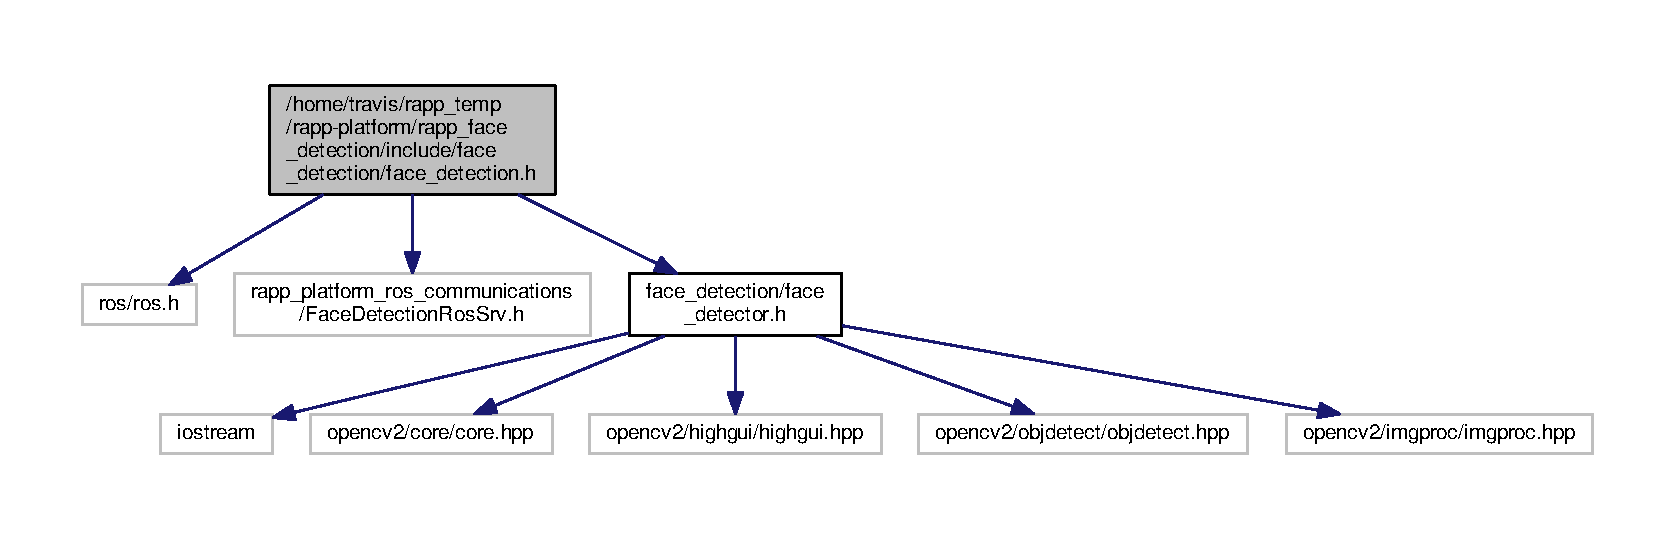
\includegraphics[width=350pt]{face__detection_8h__incl}
\end{center}
\end{figure}
This graph shows which files directly or indirectly include this file\-:
\nopagebreak
\begin{figure}[H]
\begin{center}
\leavevmode
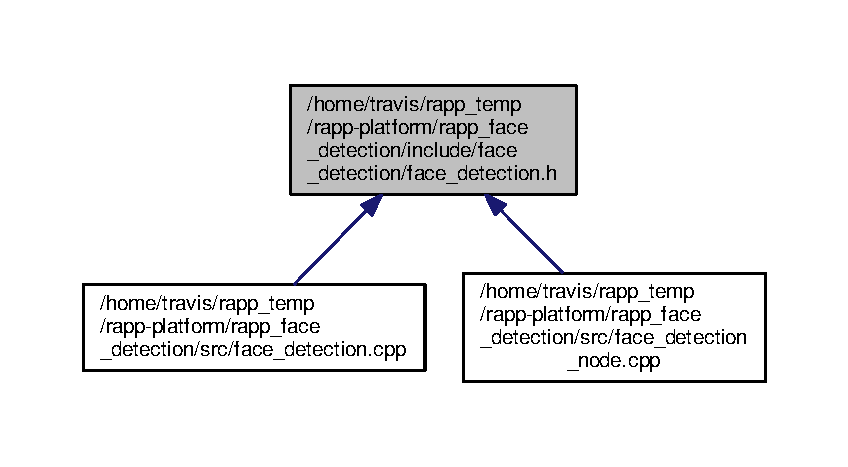
\includegraphics[width=350pt]{face__detection_8h__dep__incl}
\end{center}
\end{figure}
\subsection*{Classes}
\begin{DoxyCompactItemize}
\item 
class \hyperlink{classFaceDetection}{Face\-Detection}
\begin{DoxyCompactList}\small\item\em Class \hyperlink{classFaceDetection}{Face\-Detection} uptakes the task of handling the R\-O\-S service callbacks. \end{DoxyCompactList}\end{DoxyCompactItemize}

\hypertarget{face__detector_8h}{\section{/home/travis/rapp\-\_\-temp/rapp-\/platform/rapp\-\_\-face\-\_\-detection/include/face\-\_\-detection/face\-\_\-detector.h File Reference}
\label{face__detector_8h}\index{/home/travis/rapp\-\_\-temp/rapp-\/platform/rapp\-\_\-face\-\_\-detection/include/face\-\_\-detection/face\-\_\-detector.\-h@{/home/travis/rapp\-\_\-temp/rapp-\/platform/rapp\-\_\-face\-\_\-detection/include/face\-\_\-detection/face\-\_\-detector.\-h}}
}
{\ttfamily \#include $<$iostream$>$}\\*
{\ttfamily \#include $<$opencv2/core/core.\-hpp$>$}\\*
{\ttfamily \#include $<$opencv2/highgui/highgui.\-hpp$>$}\\*
{\ttfamily \#include $<$opencv2/objdetect/objdetect.\-hpp$>$}\\*
{\ttfamily \#include $<$opencv2/imgproc/imgproc.\-hpp$>$}\\*
Include dependency graph for face\-\_\-detector.\-h\-:
This graph shows which files directly or indirectly include this file\-:
\subsection*{Classes}
\begin{DoxyCompactItemize}
\item 
class \hyperlink{classFaceDetector}{Face\-Detector}
\begin{DoxyCompactList}\small\item\em Class that implements a face detection algorithm based on a Haar cascade classifier. \end{DoxyCompactList}\end{DoxyCompactItemize}

\hypertarget{face__detection_8cpp}{\section{/home/travis/rapp\-\_\-temp/rapp-\/platform/rapp\-\_\-face\-\_\-detection/src/face\-\_\-detection.cpp File Reference}
\label{face__detection_8cpp}\index{/home/travis/rapp\-\_\-temp/rapp-\/platform/rapp\-\_\-face\-\_\-detection/src/face\-\_\-detection.\-cpp@{/home/travis/rapp\-\_\-temp/rapp-\/platform/rapp\-\_\-face\-\_\-detection/src/face\-\_\-detection.\-cpp}}
}
{\ttfamily \#include $<$face\-\_\-detection/face\-\_\-detection.\-h$>$}\\*
Include dependency graph for face\-\_\-detection.\-cpp\-:
\nopagebreak
\begin{figure}[H]
\begin{center}
\leavevmode
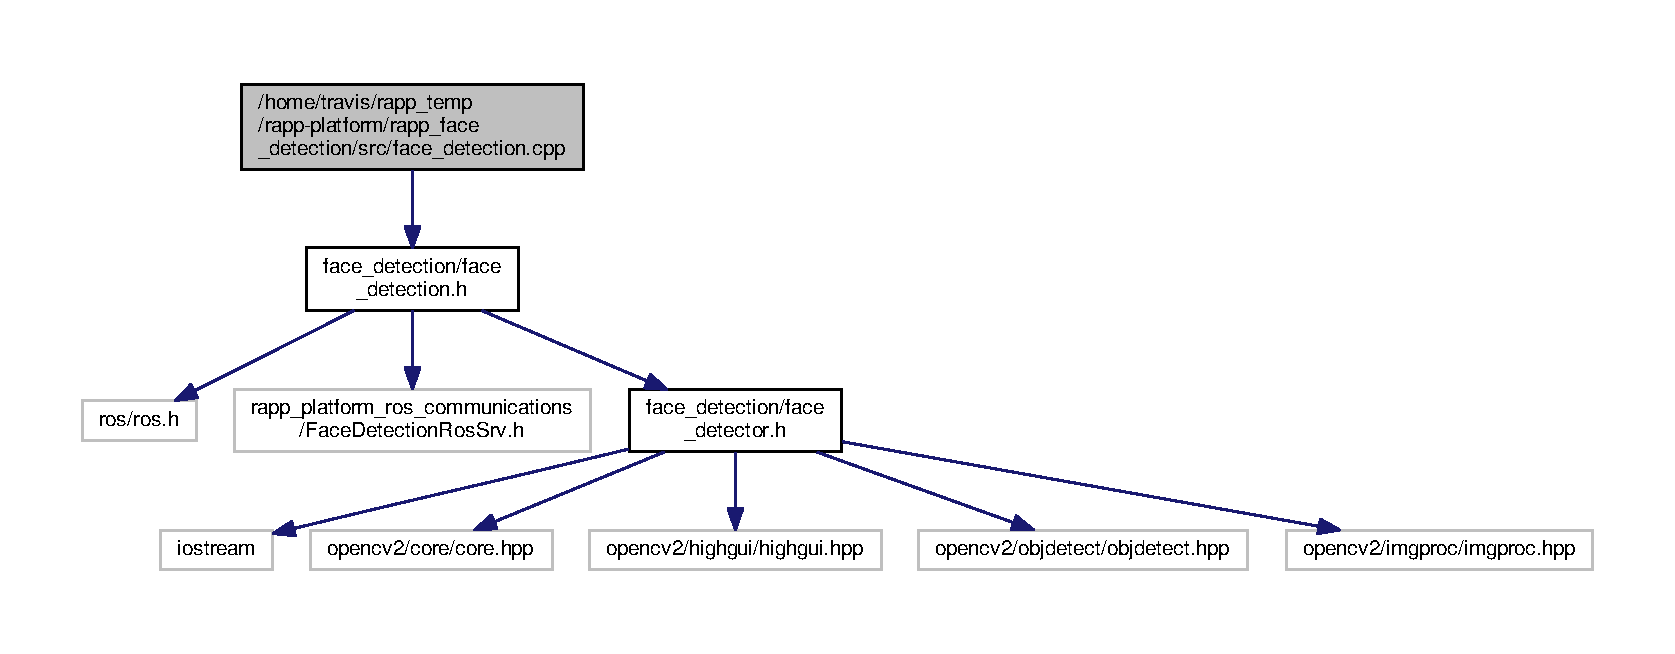
\includegraphics[width=350pt]{face__detection_8cpp__incl}
\end{center}
\end{figure}

\hypertarget{face__detection__node_8cpp}{\section{/home/travis/rapp\-\_\-temp/rapp-\/platform/rapp\-\_\-face\-\_\-detection/src/face\-\_\-detection\-\_\-node.cpp File Reference}
\label{face__detection__node_8cpp}\index{/home/travis/rapp\-\_\-temp/rapp-\/platform/rapp\-\_\-face\-\_\-detection/src/face\-\_\-detection\-\_\-node.\-cpp@{/home/travis/rapp\-\_\-temp/rapp-\/platform/rapp\-\_\-face\-\_\-detection/src/face\-\_\-detection\-\_\-node.\-cpp}}
}
{\ttfamily \#include $<$face\-\_\-detection/face\-\_\-detection.\-h$>$}\\*
Include dependency graph for face\-\_\-detection\-\_\-node.\-cpp\-:
\nopagebreak
\begin{figure}[H]
\begin{center}
\leavevmode
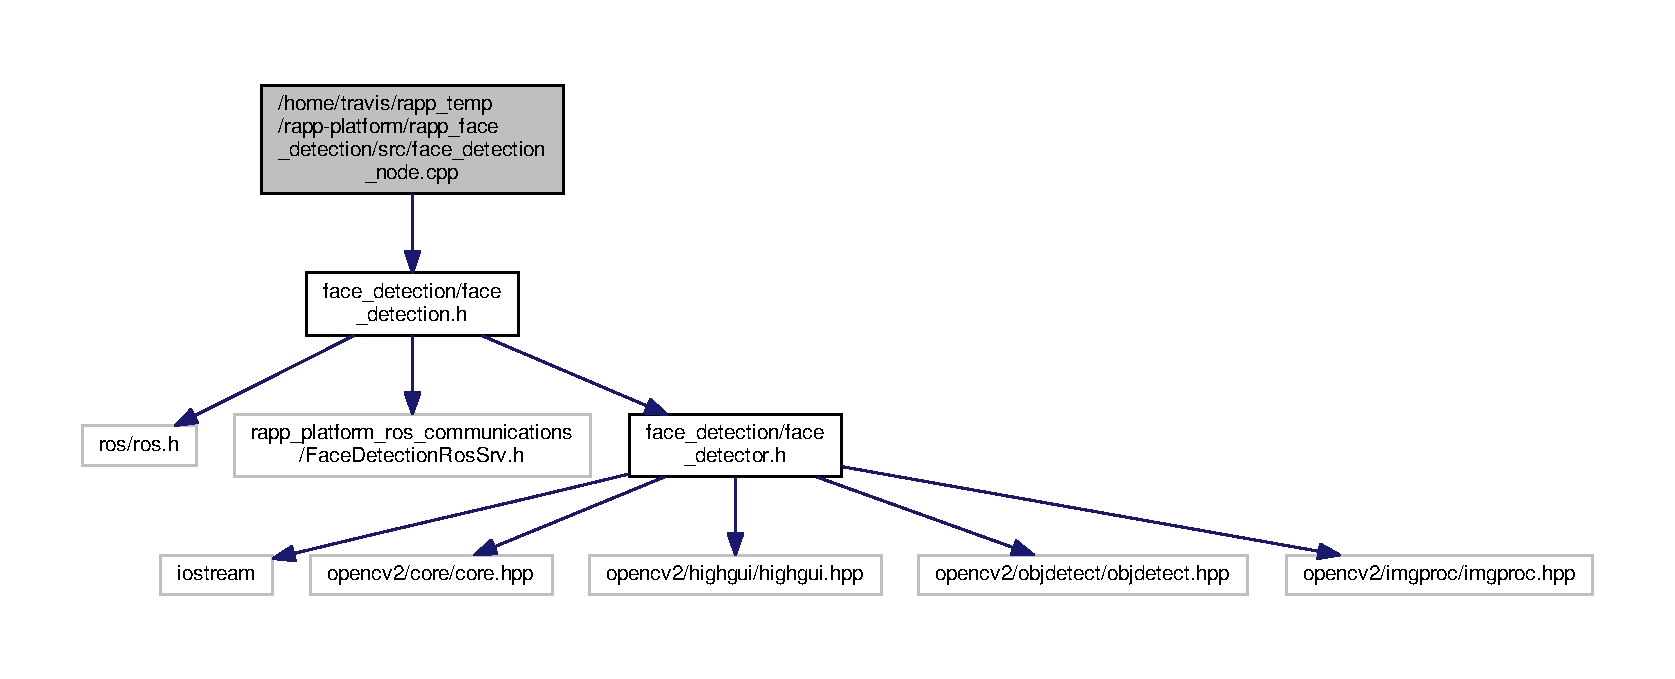
\includegraphics[width=350pt]{face__detection__node_8cpp__incl}
\end{center}
\end{figure}
\subsection*{Functions}
\begin{DoxyCompactItemize}
\item 
int \hyperlink{face__detection__node_8cpp_a3c04138a5bfe5d72780bb7e82a18e627}{main} (int argc, char $\ast$$\ast$argv)
\begin{DoxyCompactList}\small\item\em The executable's main function. Creates a R\-O\-S multispinner to enable concurrent requests and declares a \hyperlink{classFaceDetection}{Face\-Detection} object. \end{DoxyCompactList}\end{DoxyCompactItemize}


\subsection{Function Documentation}
\hypertarget{face__detection__node_8cpp_a3c04138a5bfe5d72780bb7e82a18e627}{\index{face\-\_\-detection\-\_\-node.\-cpp@{face\-\_\-detection\-\_\-node.\-cpp}!main@{main}}
\index{main@{main}!face_detection_node.cpp@{face\-\_\-detection\-\_\-node.\-cpp}}
\subsubsection[{main}]{\setlength{\rightskip}{0pt plus 5cm}int main (
\begin{DoxyParamCaption}
\item[{int}]{argc, }
\item[{char $\ast$$\ast$}]{argv}
\end{DoxyParamCaption}
)}}\label{face__detection__node_8cpp_a3c04138a5bfe5d72780bb7e82a18e627}


The executable's main function. Creates a R\-O\-S multispinner to enable concurrent requests and declares a \hyperlink{classFaceDetection}{Face\-Detection} object. 



Definition at line 24 of file face\-\_\-detection\-\_\-node.\-cpp.


\hypertarget{face__detector_8cpp}{\section{/home/travis/rapp\-\_\-temp/rapp-\/platform/rapp\-\_\-face\-\_\-detection/src/face\-\_\-detector.cpp File Reference}
\label{face__detector_8cpp}\index{/home/travis/rapp\-\_\-temp/rapp-\/platform/rapp\-\_\-face\-\_\-detection/src/face\-\_\-detector.\-cpp@{/home/travis/rapp\-\_\-temp/rapp-\/platform/rapp\-\_\-face\-\_\-detection/src/face\-\_\-detector.\-cpp}}
}
{\ttfamily \#include $<$face\-\_\-detection/face\-\_\-detector.\-h$>$}\\*
Include dependency graph for face\-\_\-detector.\-cpp\-:
\nopagebreak
\begin{figure}[H]
\begin{center}
\leavevmode
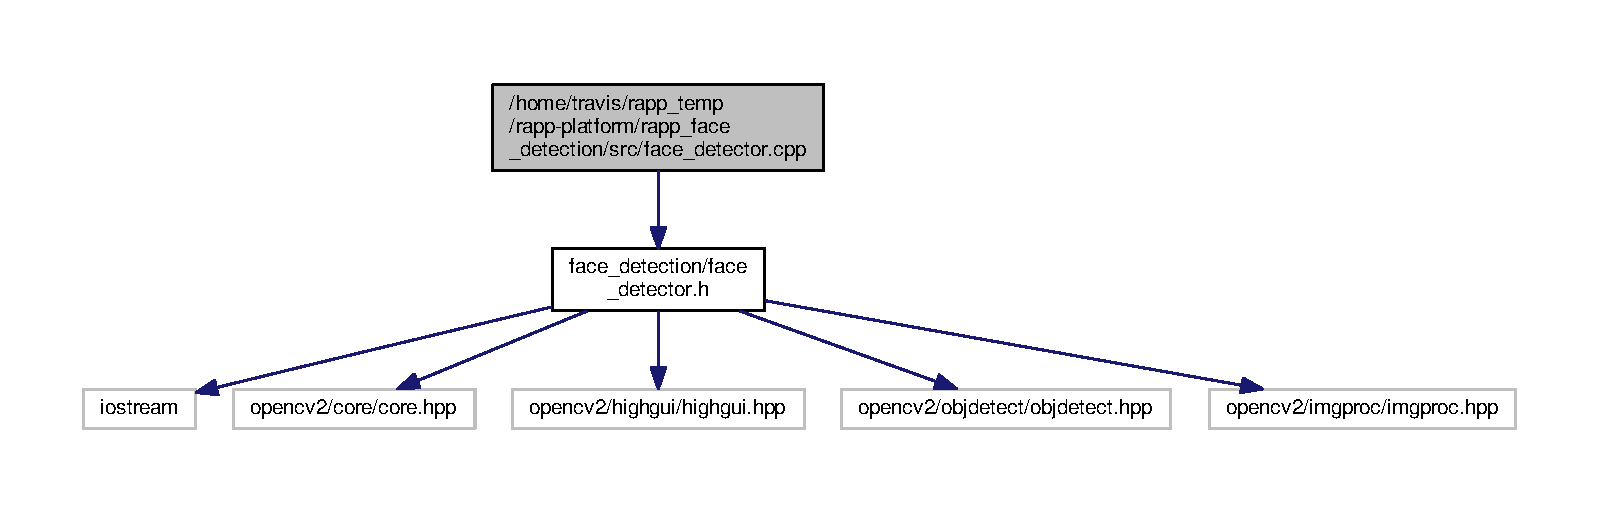
\includegraphics[width=350pt]{face__detector_8cpp__incl}
\end{center}
\end{figure}

\hypertarget{knowrob__wrapper_8h}{\section{/home/travis/rapp\-\_\-temp/rapp-\/platform/rapp\-\_\-knowrob\-\_\-wrapper/include/knowrob\-\_\-wrapper/knowrob\-\_\-wrapper.h File Reference}
\label{knowrob__wrapper_8h}\index{/home/travis/rapp\-\_\-temp/rapp-\/platform/rapp\-\_\-knowrob\-\_\-wrapper/include/knowrob\-\_\-wrapper/knowrob\-\_\-wrapper.\-h@{/home/travis/rapp\-\_\-temp/rapp-\/platform/rapp\-\_\-knowrob\-\_\-wrapper/include/knowrob\-\_\-wrapper/knowrob\-\_\-wrapper.\-h}}
}
{\ttfamily \#include $<$string$>$}\\*
{\ttfamily \#include $<$iostream$>$}\\*
{\ttfamily \#include $<$json\-\_\-prolog/prolog.\-h$>$}\\*
{\ttfamily \#include $<$rapp\-\_\-platform\-\_\-ros\-\_\-communications/register\-User\-Ontology\-Alias\-Srv.\-h$>$}\\*
{\ttfamily \#include $<$rapp\-\_\-platform\-\_\-ros\-\_\-communications/get\-User\-Ontology\-Alias\-Srv.\-h$>$}\\*
{\ttfamily \#include $<$rapp\-\_\-platform\-\_\-ros\-\_\-communications/\-String\-Array\-Msg.\-h$>$}\\*
{\ttfamily \#include $<$rapp\-\_\-platform\-\_\-ros\-\_\-communications/create\-Instance\-Srv.\-h$>$}\\*
{\ttfamily \#include $<$rapp\-\_\-platform\-\_\-ros\-\_\-communications/ontology\-Instances\-Of\-Srv.\-h$>$}\\*
{\ttfamily \#include $<$rapp\-\_\-platform\-\_\-ros\-\_\-communications/ontology\-Load\-Dump\-Srv.\-h$>$}\\*
{\ttfamily \#include $<$rapp\-\_\-platform\-\_\-ros\-\_\-communications/ontology\-Sub\-Super\-Classes\-Of\-Srv.\-h$>$}\\*
{\ttfamily \#include $<$rapp\-\_\-platform\-\_\-ros\-\_\-communications/assert\-Retract\-Attribute\-Srv.\-h$>$}\\*
{\ttfamily \#include $<$rapp\-\_\-platform\-\_\-ros\-\_\-communications/ontology\-Is\-Sub\-Super\-Class\-Of\-Srv.\-h$>$}\\*
{\ttfamily \#include $<$rapp\-\_\-platform\-\_\-ros\-\_\-communications/return\-User\-Instances\-Of\-Class\-Srv.\-h$>$}\\*
{\ttfamily \#include $<$rapp\-\_\-platform\-\_\-ros\-\_\-communications/create\-Ontology\-Alias\-Srv.\-h$>$}\\*
{\ttfamily \#include $<$rapp\-\_\-platform\-\_\-ros\-\_\-communications/user\-Performance\-Cognitve\-Tests\-Srv.\-h$>$}\\*
{\ttfamily \#include $<$rapp\-\_\-platform\-\_\-ros\-\_\-communications/create\-Cognitive\-Exercise\-Test\-Srv.\-h$>$}\\*
{\ttfamily \#include $<$rapp\-\_\-platform\-\_\-ros\-\_\-communications/cognitive\-Tests\-Of\-Type\-Srv.\-h$>$}\\*
{\ttfamily \#include $<$rapp\-\_\-platform\-\_\-ros\-\_\-communications/record\-User\-Performance\-Cognitive\-Tests\-Srv.\-h$>$}\\*
{\ttfamily \#include $<$rapp\-\_\-platform\-\_\-ros\-\_\-communications/clear\-User\-Performance\-Cognitve\-Tests\-Srv.\-h$>$}\\*
{\ttfamily \#include $<$rapp\-\_\-platform\-\_\-ros\-\_\-communications/register\-Image\-Object\-To\-Ontology\-Srv.\-h$>$}\\*
{\ttfamily \#include $<$rapp\-\_\-platform\-\_\-ros\-\_\-communications/retract\-User\-Ontology\-Alias\-Srv.\-h$>$}\\*
Include dependency graph for knowrob\-\_\-wrapper.\-h\-:
\nopagebreak
\begin{figure}[H]
\begin{center}
\leavevmode
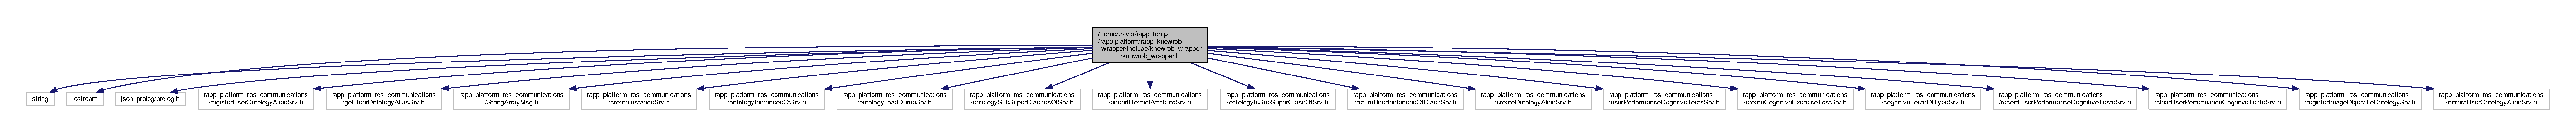
\includegraphics[width=350pt]{knowrob__wrapper_8h__incl}
\end{center}
\end{figure}
This graph shows which files directly or indirectly include this file\-:
\nopagebreak
\begin{figure}[H]
\begin{center}
\leavevmode
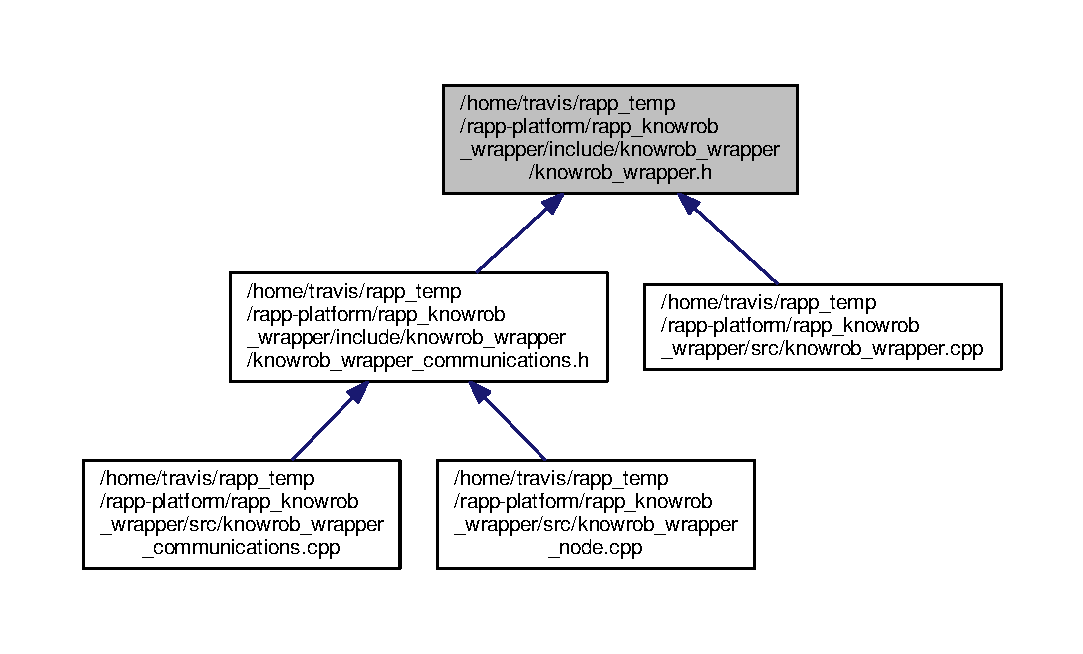
\includegraphics[width=350pt]{knowrob__wrapper_8h__dep__incl}
\end{center}
\end{figure}
\subsection*{Classes}
\begin{DoxyCompactItemize}
\item 
class \hyperlink{classKnowrobWrapper}{Knowrob\-Wrapper}
\begin{DoxyCompactList}\small\item\em Class \hyperlink{classKnowrobWrapperCommunications}{Knowrob\-Wrapper\-Communications} contains all the necessary knowrob wrapper functions. \end{DoxyCompactList}\end{DoxyCompactItemize}

\hypertarget{knowrob__wrapper__communications_8h}{\section{/home/travis/rapp\-\_\-temp/rapp-\/platform/rapp\-\_\-knowrob\-\_\-wrapper/include/knowrob\-\_\-wrapper/knowrob\-\_\-wrapper\-\_\-communications.h File Reference}
\label{knowrob__wrapper__communications_8h}\index{/home/travis/rapp\-\_\-temp/rapp-\/platform/rapp\-\_\-knowrob\-\_\-wrapper/include/knowrob\-\_\-wrapper/knowrob\-\_\-wrapper\-\_\-communications.\-h@{/home/travis/rapp\-\_\-temp/rapp-\/platform/rapp\-\_\-knowrob\-\_\-wrapper/include/knowrob\-\_\-wrapper/knowrob\-\_\-wrapper\-\_\-communications.\-h}}
}
{\ttfamily \#include $<$knowrob\-\_\-wrapper/knowrob\-\_\-wrapper.\-h$>$}\\*
{\ttfamily \#include $<$ros/ros.\-h$>$}\\*
Include dependency graph for knowrob\-\_\-wrapper\-\_\-communications.\-h\-:
This graph shows which files directly or indirectly include this file\-:
\subsection*{Classes}
\begin{DoxyCompactItemize}
\item 
class \hyperlink{classKnowrobWrapperCommunications}{Knowrob\-Wrapper\-Communications}
\begin{DoxyCompactList}\small\item\em Class \hyperlink{classKnowrobWrapperCommunications}{Knowrob\-Wrapper\-Communications} uptakes the task of handling the R\-O\-S service callbacks. \end{DoxyCompactList}\end{DoxyCompactItemize}

\hypertarget{knowrob__wrapper_8cpp}{\section{/home/travis/rapp\-\_\-temp/rapp-\/platform/rapp\-\_\-knowrob\-\_\-wrapper/src/knowrob\-\_\-wrapper.cpp File Reference}
\label{knowrob__wrapper_8cpp}\index{/home/travis/rapp\-\_\-temp/rapp-\/platform/rapp\-\_\-knowrob\-\_\-wrapper/src/knowrob\-\_\-wrapper.\-cpp@{/home/travis/rapp\-\_\-temp/rapp-\/platform/rapp\-\_\-knowrob\-\_\-wrapper/src/knowrob\-\_\-wrapper.\-cpp}}
}
{\ttfamily \#include $<$knowrob\-\_\-wrapper/knowrob\-\_\-wrapper.\-h$>$}\\*
{\ttfamily \#include $<$sys/stat.\-h$>$}\\*
{\ttfamily \#include $<$unistd.\-h$>$}\\*
{\ttfamily \#include $<$sstream$>$}\\*
{\ttfamily \#include $<$ros/package.\-h$>$}\\*
{\ttfamily \#include $<$fstream$>$}\\*
Include dependency graph for knowrob\-\_\-wrapper.\-cpp\-:
\nopagebreak
\begin{figure}[H]
\begin{center}
\leavevmode
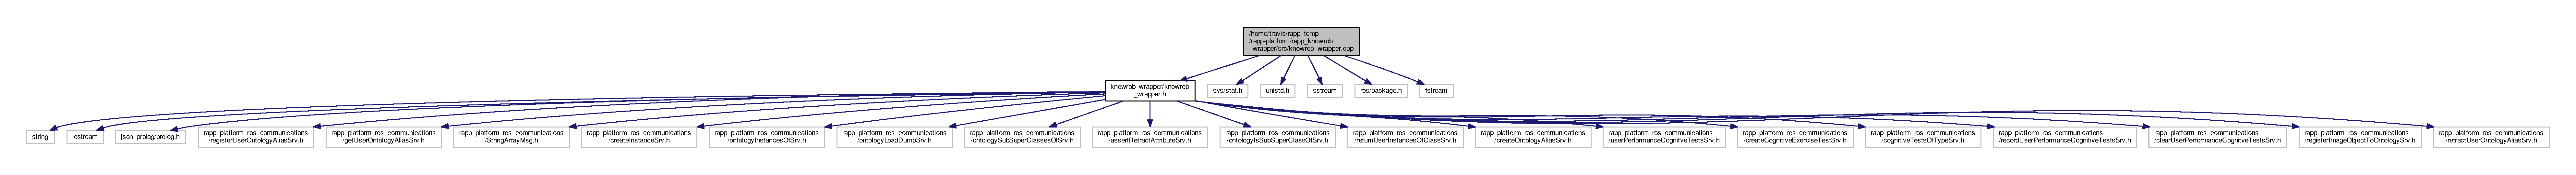
\includegraphics[width=350pt]{knowrob__wrapper_8cpp__incl}
\end{center}
\end{figure}
\subsection*{Functions}
\begin{DoxyCompactItemize}
\item 
bool \hyperlink{knowrob__wrapper_8cpp_a1d733fb67ce063a4ec39598ed92b9934}{check\-If\-File\-Exists} (const char $\ast$file\-Name)
\begin{DoxyCompactList}\small\item\em Checks if path exists. \end{DoxyCompactList}\item 
std\-::string \hyperlink{knowrob__wrapper_8cpp_aaf197f973c9edcca9610fba8b86df471}{int\-To\-String} (int a)
\begin{DoxyCompactList}\small\item\em Converts integer to string. \end{DoxyCompactList}\item 
std\-::vector$<$ std\-::string $>$ \hyperlink{knowrob__wrapper_8cpp_a527876ebdba0ec57bd96287221b4a594}{split} (std\-::string str, std\-::string sep)
\begin{DoxyCompactList}\small\item\em Splits string by delimiter. \end{DoxyCompactList}\item 
std\-::string \hyperlink{knowrob__wrapper_8cpp_abe4875a997df10557ec66d950b0bcb53}{Split\-Filename} (const std\-::string \&str)
\begin{DoxyCompactList}\small\item\em Keeps only the final folder or file from a path. \end{DoxyCompactList}\end{DoxyCompactItemize}


\subsection{Function Documentation}
\hypertarget{knowrob__wrapper_8cpp_a1d733fb67ce063a4ec39598ed92b9934}{\index{knowrob\-\_\-wrapper.\-cpp@{knowrob\-\_\-wrapper.\-cpp}!check\-If\-File\-Exists@{check\-If\-File\-Exists}}
\index{check\-If\-File\-Exists@{check\-If\-File\-Exists}!knowrob_wrapper.cpp@{knowrob\-\_\-wrapper.\-cpp}}
\subsubsection[{check\-If\-File\-Exists}]{\setlength{\rightskip}{0pt plus 5cm}bool check\-If\-File\-Exists (
\begin{DoxyParamCaption}
\item[{const char $\ast$}]{file\-Name}
\end{DoxyParamCaption}
)}}\label{knowrob__wrapper_8cpp_a1d733fb67ce063a4ec39598ed92b9934}


Checks if path exists. 


\begin{DoxyParams}{Parameters}
{\em file\-Name} & \mbox{[}char$\ast$\mbox{]} The input path \\
\hline
\end{DoxyParams}
\begin{DoxyReturn}{Returns}
out \mbox{[}bool\mbox{]} True if file exists 
\end{DoxyReturn}


Definition at line 66 of file knowrob\-\_\-wrapper.\-cpp.

\hypertarget{knowrob__wrapper_8cpp_aaf197f973c9edcca9610fba8b86df471}{\index{knowrob\-\_\-wrapper.\-cpp@{knowrob\-\_\-wrapper.\-cpp}!int\-To\-String@{int\-To\-String}}
\index{int\-To\-String@{int\-To\-String}!knowrob_wrapper.cpp@{knowrob\-\_\-wrapper.\-cpp}}
\subsubsection[{int\-To\-String}]{\setlength{\rightskip}{0pt plus 5cm}std\-::string int\-To\-String (
\begin{DoxyParamCaption}
\item[{int}]{a}
\end{DoxyParamCaption}
)}}\label{knowrob__wrapper_8cpp_aaf197f973c9edcca9610fba8b86df471}


Converts integer to string. 


\begin{DoxyParams}{Parameters}
{\em a} & \mbox{[}int\mbox{]} The input integer \\
\hline
\end{DoxyParams}
\begin{DoxyReturn}{Returns}
out \mbox{[}string\mbox{]} The output string 
\end{DoxyReturn}


Definition at line 42 of file knowrob\-\_\-wrapper.\-cpp.

\hypertarget{knowrob__wrapper_8cpp_a527876ebdba0ec57bd96287221b4a594}{\index{knowrob\-\_\-wrapper.\-cpp@{knowrob\-\_\-wrapper.\-cpp}!split@{split}}
\index{split@{split}!knowrob_wrapper.cpp@{knowrob\-\_\-wrapper.\-cpp}}
\subsubsection[{split}]{\setlength{\rightskip}{0pt plus 5cm}std\-::vector$<$std\-::string$>$ split (
\begin{DoxyParamCaption}
\item[{std\-::string}]{str, }
\item[{std\-::string}]{sep}
\end{DoxyParamCaption}
)}}\label{knowrob__wrapper_8cpp_a527876ebdba0ec57bd96287221b4a594}


Splits string by delimiter. 


\begin{DoxyParams}{Parameters}
{\em str} & \mbox{[}string\mbox{]} The input string \\
\hline
{\em sep} & \mbox{[}string\mbox{]} The delimiter \\
\hline
\end{DoxyParams}
\begin{DoxyReturn}{Returns}
arr \mbox{[}std\-::vector$<$std\-::string$>$\mbox{]} A vector with the string parts as splitted by the delimiter 
\end{DoxyReturn}


Definition at line 78 of file knowrob\-\_\-wrapper.\-cpp.

\hypertarget{knowrob__wrapper_8cpp_abe4875a997df10557ec66d950b0bcb53}{\index{knowrob\-\_\-wrapper.\-cpp@{knowrob\-\_\-wrapper.\-cpp}!Split\-Filename@{Split\-Filename}}
\index{Split\-Filename@{Split\-Filename}!knowrob_wrapper.cpp@{knowrob\-\_\-wrapper.\-cpp}}
\subsubsection[{Split\-Filename}]{\setlength{\rightskip}{0pt plus 5cm}std\-::string Split\-Filename (
\begin{DoxyParamCaption}
\item[{const std\-::string \&}]{str}
\end{DoxyParamCaption}
)}}\label{knowrob__wrapper_8cpp_abe4875a997df10557ec66d950b0bcb53}


Keeps only the final folder or file from a path. 


\begin{DoxyParams}{Parameters}
{\em str} & \mbox{[}string\&\mbox{]} The input path \\
\hline
\end{DoxyParams}
\begin{DoxyReturn}{Returns}
out \mbox{[}string\mbox{]} The output filename 
\end{DoxyReturn}


Definition at line 54 of file knowrob\-\_\-wrapper.\-cpp.


\hypertarget{knowrob__wrapper__communications_8cpp}{\section{/home/travis/rapp\-\_\-temp/rapp-\/platform/rapp\-\_\-knowrob\-\_\-wrapper/src/knowrob\-\_\-wrapper\-\_\-communications.cpp File Reference}
\label{knowrob__wrapper__communications_8cpp}\index{/home/travis/rapp\-\_\-temp/rapp-\/platform/rapp\-\_\-knowrob\-\_\-wrapper/src/knowrob\-\_\-wrapper\-\_\-communications.\-cpp@{/home/travis/rapp\-\_\-temp/rapp-\/platform/rapp\-\_\-knowrob\-\_\-wrapper/src/knowrob\-\_\-wrapper\-\_\-communications.\-cpp}}
}
{\ttfamily \#include $<$knowrob\-\_\-wrapper/knowrob\-\_\-wrapper\-\_\-communications.\-h$>$}\\*
{\ttfamily \#include $<$ros/package.\-h$>$}\\*
Include dependency graph for knowrob\-\_\-wrapper\-\_\-communications.\-cpp\-:

\hypertarget{knowrob__wrapper__node_8cpp}{\section{/home/travis/rapp\-\_\-temp/rapp-\/platform/rapp\-\_\-knowrob\-\_\-wrapper/src/knowrob\-\_\-wrapper\-\_\-node.cpp File Reference}
\label{knowrob__wrapper__node_8cpp}\index{/home/travis/rapp\-\_\-temp/rapp-\/platform/rapp\-\_\-knowrob\-\_\-wrapper/src/knowrob\-\_\-wrapper\-\_\-node.\-cpp@{/home/travis/rapp\-\_\-temp/rapp-\/platform/rapp\-\_\-knowrob\-\_\-wrapper/src/knowrob\-\_\-wrapper\-\_\-node.\-cpp}}
}
{\ttfamily \#include $<$knowrob\-\_\-wrapper/knowrob\-\_\-wrapper\-\_\-communications.\-h$>$}\\*
Include dependency graph for knowrob\-\_\-wrapper\-\_\-node.\-cpp\-:
\nopagebreak
\begin{figure}[H]
\begin{center}
\leavevmode
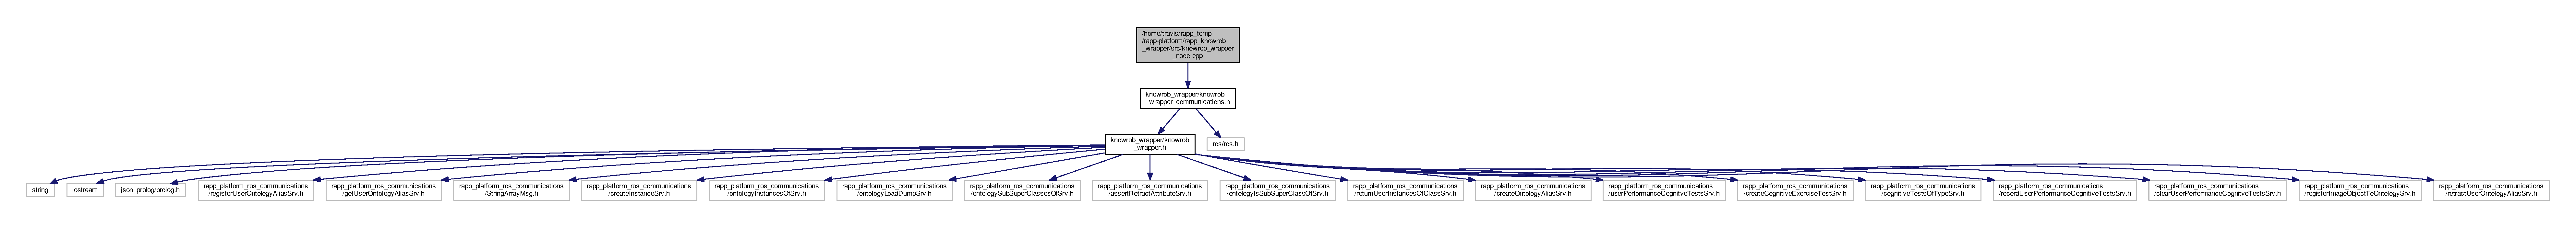
\includegraphics[width=350pt]{knowrob__wrapper__node_8cpp__incl}
\end{center}
\end{figure}
\subsection*{Functions}
\begin{DoxyCompactItemize}
\item 
int \hyperlink{knowrob__wrapper__node_8cpp_a3c04138a5bfe5d72780bb7e82a18e627}{main} (int argc, char $\ast$$\ast$argv)
\begin{DoxyCompactList}\small\item\em The executable's main function. Creates a R\-O\-S multispinner to enable concurrent requests and declares a \hyperlink{classKnowrobWrapperCommunications}{Knowrob\-Wrapper\-Communications} object. \end{DoxyCompactList}\end{DoxyCompactItemize}


\subsection{Function Documentation}
\hypertarget{knowrob__wrapper__node_8cpp_a3c04138a5bfe5d72780bb7e82a18e627}{\index{knowrob\-\_\-wrapper\-\_\-node.\-cpp@{knowrob\-\_\-wrapper\-\_\-node.\-cpp}!main@{main}}
\index{main@{main}!knowrob_wrapper_node.cpp@{knowrob\-\_\-wrapper\-\_\-node.\-cpp}}
\subsubsection[{main}]{\setlength{\rightskip}{0pt plus 5cm}int main (
\begin{DoxyParamCaption}
\item[{int}]{argc, }
\item[{char $\ast$$\ast$}]{argv}
\end{DoxyParamCaption}
)}}\label{knowrob__wrapper__node_8cpp_a3c04138a5bfe5d72780bb7e82a18e627}


The executable's main function. Creates a R\-O\-S multispinner to enable concurrent requests and declares a \hyperlink{classKnowrobWrapperCommunications}{Knowrob\-Wrapper\-Communications} object. 



Definition at line 27 of file knowrob\-\_\-wrapper\-\_\-node.\-cpp.


\hypertarget{mysql__wrapper_8py}{\section{/home/travis/rapp\-\_\-temp/rapp-\/platform/rapp\-\_\-mysql\-\_\-wrapper/src/mysql\-\_\-wrapper.py File Reference}
\label{mysql__wrapper_8py}\index{/home/travis/rapp\-\_\-temp/rapp-\/platform/rapp\-\_\-mysql\-\_\-wrapper/src/mysql\-\_\-wrapper.\-py@{/home/travis/rapp\-\_\-temp/rapp-\/platform/rapp\-\_\-mysql\-\_\-wrapper/src/mysql\-\_\-wrapper.\-py}}
}
\subsection*{Classes}
\begin{DoxyCompactItemize}
\item 
class \hyperlink{classmysql__wrapper_1_1MySQLdbWrapper}{mysql\-\_\-wrapper.\-My\-S\-Q\-Ldb\-Wrapper}
\begin{DoxyCompactList}\small\item\em The mysql wrapper ros node. \end{DoxyCompactList}\end{DoxyCompactItemize}
\subsection*{Namespaces}
\begin{DoxyCompactItemize}
\item 
\hyperlink{namespacemysql__wrapper}{mysql\-\_\-wrapper}
\end{DoxyCompactItemize}

\hypertarget{mysql__wrapper__main_8py}{\section{/home/travis/rapp\-\_\-temp/rapp-\/platform/rapp\-\_\-mysql\-\_\-wrapper/src/mysql\-\_\-wrapper\-\_\-main.py File Reference}
\label{mysql__wrapper__main_8py}\index{/home/travis/rapp\-\_\-temp/rapp-\/platform/rapp\-\_\-mysql\-\_\-wrapper/src/mysql\-\_\-wrapper\-\_\-main.\-py@{/home/travis/rapp\-\_\-temp/rapp-\/platform/rapp\-\_\-mysql\-\_\-wrapper/src/mysql\-\_\-wrapper\-\_\-main.\-py}}
}
\subsection*{Namespaces}
\begin{DoxyCompactItemize}
\item 
\hyperlink{namespacemysql__wrapper__main}{mysql\-\_\-wrapper\-\_\-main}
\end{DoxyCompactItemize}
\subsection*{Variables}
\begin{DoxyCompactItemize}
\item 
tuple \hyperlink{namespacemysql__wrapper__main_a168b1afc2608b144cd98ea4aac4b4639}{mysql\-\_\-wrapper\-\_\-main.\-My\-S\-Q\-L\-Wrapper\-Node} = My\-S\-Q\-Ldb\-Wrapper()
\begin{DoxyCompactList}\small\item\em The main function that initiates the rapp mysql wrapper R\-O\-S Node. \end{DoxyCompactList}\end{DoxyCompactItemize}

\hypertarget{qr__detection_8h}{\section{/home/travis/rapp\-\_\-temp/rapp-\/platform/rapp\-\_\-qr\-\_\-detection/include/qr\-\_\-detection/qr\-\_\-detection.h File Reference}
\label{qr__detection_8h}\index{/home/travis/rapp\-\_\-temp/rapp-\/platform/rapp\-\_\-qr\-\_\-detection/include/qr\-\_\-detection/qr\-\_\-detection.\-h@{/home/travis/rapp\-\_\-temp/rapp-\/platform/rapp\-\_\-qr\-\_\-detection/include/qr\-\_\-detection/qr\-\_\-detection.\-h}}
}
{\ttfamily \#include \char`\"{}ros/ros.\-h\char`\"{}}\\*
{\ttfamily \#include $<$rapp\-\_\-platform\-\_\-ros\-\_\-communications/\-Qr\-Detection\-Ros\-Srv.\-h$>$}\\*
{\ttfamily \#include $<$qr\-\_\-detection/qr\-\_\-detector.\-h$>$}\\*
Include dependency graph for qr\-\_\-detection.\-h\-:
\nopagebreak
\begin{figure}[H]
\begin{center}
\leavevmode
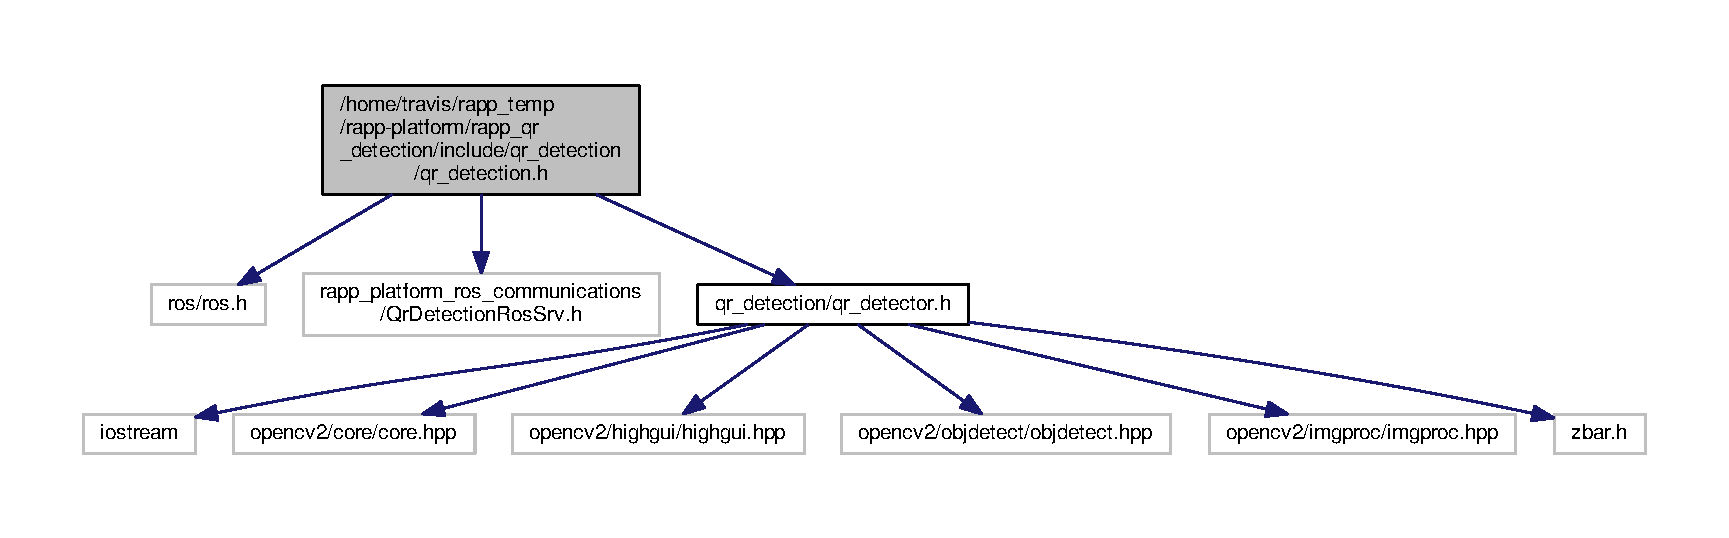
\includegraphics[width=350pt]{qr__detection_8h__incl}
\end{center}
\end{figure}
This graph shows which files directly or indirectly include this file\-:
\nopagebreak
\begin{figure}[H]
\begin{center}
\leavevmode
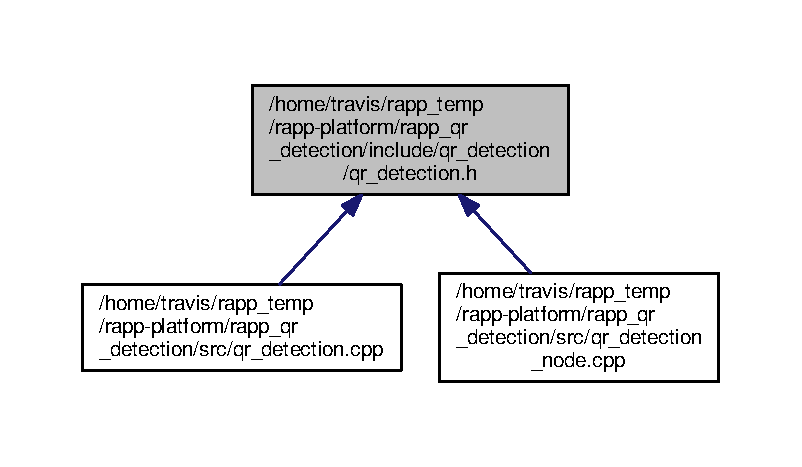
\includegraphics[width=350pt]{qr__detection_8h__dep__incl}
\end{center}
\end{figure}
\subsection*{Classes}
\begin{DoxyCompactItemize}
\item 
class \hyperlink{classQrDetection}{Qr\-Detection}
\begin{DoxyCompactList}\small\item\em Uptakes the task of setting up the R\-O\-S service callbacks towards qr detection. \end{DoxyCompactList}\end{DoxyCompactItemize}

\hypertarget{qr__detector_8h}{\section{/home/travis/rapp\-\_\-temp/rapp-\/platform/rapp\-\_\-qr\-\_\-detection/include/qr\-\_\-detection/qr\-\_\-detector.h File Reference}
\label{qr__detector_8h}\index{/home/travis/rapp\-\_\-temp/rapp-\/platform/rapp\-\_\-qr\-\_\-detection/include/qr\-\_\-detection/qr\-\_\-detector.\-h@{/home/travis/rapp\-\_\-temp/rapp-\/platform/rapp\-\_\-qr\-\_\-detection/include/qr\-\_\-detection/qr\-\_\-detector.\-h}}
}
{\ttfamily \#include $<$iostream$>$}\\*
{\ttfamily \#include $<$opencv2/core/core.\-hpp$>$}\\*
{\ttfamily \#include $<$opencv2/highgui/highgui.\-hpp$>$}\\*
{\ttfamily \#include $<$opencv2/objdetect/objdetect.\-hpp$>$}\\*
{\ttfamily \#include $<$opencv2/imgproc/imgproc.\-hpp$>$}\\*
{\ttfamily \#include $<$zbar.\-h$>$}\\*
Include dependency graph for qr\-\_\-detector.\-h\-:
This graph shows which files directly or indirectly include this file\-:
\subsection*{Classes}
\begin{DoxyCompactItemize}
\item 
class \hyperlink{structQrCode}{Qr\-Code}
\begin{DoxyCompactList}\small\item\em Structure holding the essential info for a Q\-R code. \end{DoxyCompactList}\item 
class \hyperlink{classQrDetector}{Qr\-Detector}
\begin{DoxyCompactList}\small\item\em Provides the Q\-R detection functionality. \end{DoxyCompactList}\end{DoxyCompactItemize}

\hypertarget{qr__detection_8cpp}{\section{/home/travis/rapp\-\_\-temp/rapp-\/platform/rapp\-\_\-qr\-\_\-detection/src/qr\-\_\-detection.cpp File Reference}
\label{qr__detection_8cpp}\index{/home/travis/rapp\-\_\-temp/rapp-\/platform/rapp\-\_\-qr\-\_\-detection/src/qr\-\_\-detection.\-cpp@{/home/travis/rapp\-\_\-temp/rapp-\/platform/rapp\-\_\-qr\-\_\-detection/src/qr\-\_\-detection.\-cpp}}
}
{\ttfamily \#include $<$qr\-\_\-detection/qr\-\_\-detection.\-h$>$}\\*
Include dependency graph for qr\-\_\-detection.\-cpp\-:

\hypertarget{qr__detection__node_8cpp}{\section{/home/travis/rapp\-\_\-temp/rapp-\/platform/rapp\-\_\-qr\-\_\-detection/src/qr\-\_\-detection\-\_\-node.cpp File Reference}
\label{qr__detection__node_8cpp}\index{/home/travis/rapp\-\_\-temp/rapp-\/platform/rapp\-\_\-qr\-\_\-detection/src/qr\-\_\-detection\-\_\-node.\-cpp@{/home/travis/rapp\-\_\-temp/rapp-\/platform/rapp\-\_\-qr\-\_\-detection/src/qr\-\_\-detection\-\_\-node.\-cpp}}
}
{\ttfamily \#include $<$qr\-\_\-detection/qr\-\_\-detection.\-h$>$}\\*
Include dependency graph for qr\-\_\-detection\-\_\-node.\-cpp\-:
\subsection*{Functions}
\begin{DoxyCompactItemize}
\item 
int \hyperlink{qr__detection__node_8cpp_a3c04138a5bfe5d72780bb7e82a18e627}{main} (int argc, char $\ast$$\ast$argv)
\begin{DoxyCompactList}\small\item\em The main function. Retrieves the threads parameter in order to enable concurrent service invocation. \end{DoxyCompactList}\end{DoxyCompactItemize}


\subsection{Function Documentation}
\hypertarget{qr__detection__node_8cpp_a3c04138a5bfe5d72780bb7e82a18e627}{\index{qr\-\_\-detection\-\_\-node.\-cpp@{qr\-\_\-detection\-\_\-node.\-cpp}!main@{main}}
\index{main@{main}!qr_detection_node.cpp@{qr\-\_\-detection\-\_\-node.\-cpp}}
\subsubsection[{main}]{\setlength{\rightskip}{0pt plus 5cm}int main (
\begin{DoxyParamCaption}
\item[{int}]{argc, }
\item[{char $\ast$$\ast$}]{argv}
\end{DoxyParamCaption}
)}}\label{qr__detection__node_8cpp_a3c04138a5bfe5d72780bb7e82a18e627}


The main function. Retrieves the threads parameter in order to enable concurrent service invocation. 



Definition at line 25 of file qr\-\_\-detection\-\_\-node.\-cpp.


\hypertarget{qr__detector_8cpp}{\section{/home/travis/rapp\-\_\-temp/rapp-\/platform/rapp\-\_\-qr\-\_\-detection/src/qr\-\_\-detector.cpp File Reference}
\label{qr__detector_8cpp}\index{/home/travis/rapp\-\_\-temp/rapp-\/platform/rapp\-\_\-qr\-\_\-detection/src/qr\-\_\-detector.\-cpp@{/home/travis/rapp\-\_\-temp/rapp-\/platform/rapp\-\_\-qr\-\_\-detection/src/qr\-\_\-detector.\-cpp}}
}
{\ttfamily \#include $<$qr\-\_\-detection/qr\-\_\-detector.\-h$>$}\\*
Include dependency graph for qr\-\_\-detector.\-cpp\-:
\nopagebreak
\begin{figure}[H]
\begin{center}
\leavevmode
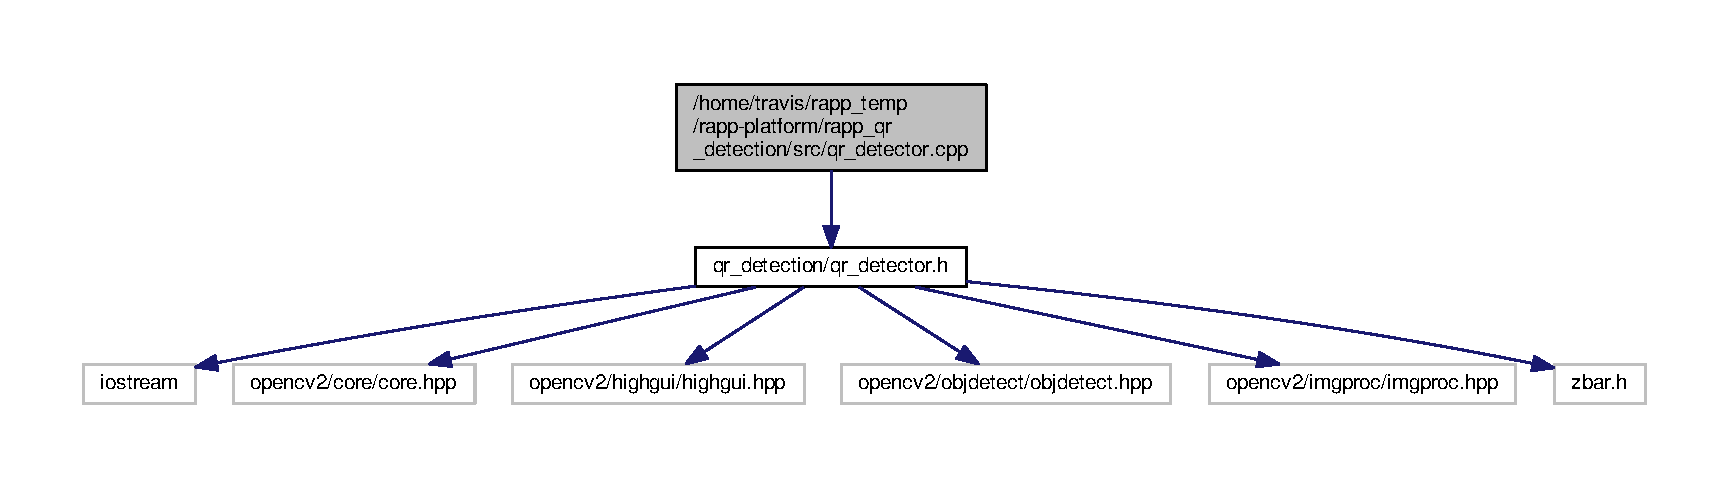
\includegraphics[width=350pt]{qr__detector_8cpp__incl}
\end{center}
\end{figure}

\hypertarget{rapp__speech__detection__google_2src_2rapp__exceptions_8py}{\section{/home/travis/rapp\-\_\-temp/rapp-\/platform/rapp\-\_\-speech\-\_\-detection\-\_\-google/src/rapp\-\_\-exceptions.py File Reference}
\label{rapp__speech__detection__google_2src_2rapp__exceptions_8py}\index{/home/travis/rapp\-\_\-temp/rapp-\/platform/rapp\-\_\-speech\-\_\-detection\-\_\-google/src/rapp\-\_\-exceptions.\-py@{/home/travis/rapp\-\_\-temp/rapp-\/platform/rapp\-\_\-speech\-\_\-detection\-\_\-google/src/rapp\-\_\-exceptions.\-py}}
}
\subsection*{Classes}
\begin{DoxyCompactItemize}
\item 
class \hyperlink{classrapp__exceptions_1_1RappError}{rapp\-\_\-exceptions.\-Rapp\-Error}
\begin{DoxyCompactList}\small\item\em Inherits Exception and is used to catch only R\-A\-P\-P-\/specific exceptions. \end{DoxyCompactList}\end{DoxyCompactItemize}
\subsection*{Namespaces}
\begin{DoxyCompactItemize}
\item 
\hyperlink{namespacerapp__exceptions}{rapp\-\_\-exceptions}
\end{DoxyCompactItemize}

\hypertarget{rapp__speech__detection__sphinx4_2src_2rapp__speech__detection__sphinx4_2rapp__exceptions_8py}{\section{/home/travis/rapp\-\_\-temp/rapp-\/platform/rapp\-\_\-speech\-\_\-detection\-\_\-sphinx4/src/rapp\-\_\-speech\-\_\-detection\-\_\-sphinx4/rapp\-\_\-exceptions.py File Reference}
\label{rapp__speech__detection__sphinx4_2src_2rapp__speech__detection__sphinx4_2rapp__exceptions_8py}\index{/home/travis/rapp\-\_\-temp/rapp-\/platform/rapp\-\_\-speech\-\_\-detection\-\_\-sphinx4/src/rapp\-\_\-speech\-\_\-detection\-\_\-sphinx4/rapp\-\_\-exceptions.\-py@{/home/travis/rapp\-\_\-temp/rapp-\/platform/rapp\-\_\-speech\-\_\-detection\-\_\-sphinx4/src/rapp\-\_\-speech\-\_\-detection\-\_\-sphinx4/rapp\-\_\-exceptions.\-py}}
}
\subsection*{Classes}
\begin{DoxyCompactItemize}
\item 
class \hyperlink{classrapp__speech__detection__sphinx4_1_1rapp__exceptions_1_1RappError}{rapp\-\_\-speech\-\_\-detection\-\_\-sphinx4.\-rapp\-\_\-exceptions.\-Rapp\-Error}
\begin{DoxyCompactList}\small\item\em Provides a R\-A\-P\-P specific exception. \end{DoxyCompactList}\end{DoxyCompactItemize}
\subsection*{Namespaces}
\begin{DoxyCompactItemize}
\item 
\hyperlink{namespacerapp__speech__detection__sphinx4_1_1rapp__exceptions}{rapp\-\_\-speech\-\_\-detection\-\_\-sphinx4.\-rapp\-\_\-exceptions}
\end{DoxyCompactItemize}

\hypertarget{rapp__text__to__speech__espeak_2src_2rapp__exceptions_8py}{\section{/home/travis/rapp\-\_\-temp/rapp-\/platform/rapp\-\_\-text\-\_\-to\-\_\-speech\-\_\-espeak/src/rapp\-\_\-exceptions.py File Reference}
\label{rapp__text__to__speech__espeak_2src_2rapp__exceptions_8py}\index{/home/travis/rapp\-\_\-temp/rapp-\/platform/rapp\-\_\-text\-\_\-to\-\_\-speech\-\_\-espeak/src/rapp\-\_\-exceptions.\-py@{/home/travis/rapp\-\_\-temp/rapp-\/platform/rapp\-\_\-text\-\_\-to\-\_\-speech\-\_\-espeak/src/rapp\-\_\-exceptions.\-py}}
}
\subsection*{Classes}
\begin{DoxyCompactItemize}
\item 
class \hyperlink{classrapp__exceptions_1_1RappError}{rapp\-\_\-exceptions.\-Rapp\-Error}
\begin{DoxyCompactList}\small\item\em Inherits Exception and is used to catch only R\-A\-P\-P-\/specific exceptions. \end{DoxyCompactList}\end{DoxyCompactItemize}
\subsection*{Namespaces}
\begin{DoxyCompactItemize}
\item 
\hyperlink{namespacerapp__exceptions}{rapp\-\_\-exceptions}
\end{DoxyCompactItemize}

\hypertarget{speech__recognition__google_8py}{\section{/home/travis/rapp\-\_\-temp/rapp-\/platform/rapp\-\_\-speech\-\_\-detection\-\_\-google/src/speech\-\_\-recognition\-\_\-google.py File Reference}
\label{speech__recognition__google_8py}\index{/home/travis/rapp\-\_\-temp/rapp-\/platform/rapp\-\_\-speech\-\_\-detection\-\_\-google/src/speech\-\_\-recognition\-\_\-google.\-py@{/home/travis/rapp\-\_\-temp/rapp-\/platform/rapp\-\_\-speech\-\_\-detection\-\_\-google/src/speech\-\_\-recognition\-\_\-google.\-py}}
}
\subsection*{Classes}
\begin{DoxyCompactItemize}
\item 
class \hyperlink{classspeech__recognition__google_1_1SpeechToTextGoogle}{speech\-\_\-recognition\-\_\-google.\-Speech\-To\-Text\-Google}
\begin{DoxyCompactList}\small\item\em Implements calls the Google A\-S\-R A\-P\-I. \end{DoxyCompactList}\end{DoxyCompactItemize}
\subsection*{Namespaces}
\begin{DoxyCompactItemize}
\item 
\hyperlink{namespacespeech__recognition__google}{speech\-\_\-recognition\-\_\-google}
\end{DoxyCompactItemize}
\subsection*{Variables}
\begin{DoxyCompactItemize}
\item 
tuple \hyperlink{namespacespeech__recognition__google_a72262ab039ae77c265a0575478792276}{speech\-\_\-recognition\-\_\-google.\-speech\-\_\-to\-\_\-text\-\_\-node} = Speech\-To\-Text\-Google()
\begin{DoxyCompactList}\small\item\em The main function. \end{DoxyCompactList}\end{DoxyCompactItemize}

\hypertarget{english__support_8py}{\section{/home/travis/rapp\-\_\-temp/rapp-\/platform/rapp\-\_\-speech\-\_\-detection\-\_\-sphinx4/src/rapp\-\_\-speech\-\_\-detection\-\_\-sphinx4/english\-\_\-support.py File Reference}
\label{english__support_8py}\index{/home/travis/rapp\-\_\-temp/rapp-\/platform/rapp\-\_\-speech\-\_\-detection\-\_\-sphinx4/src/rapp\-\_\-speech\-\_\-detection\-\_\-sphinx4/english\-\_\-support.\-py@{/home/travis/rapp\-\_\-temp/rapp-\/platform/rapp\-\_\-speech\-\_\-detection\-\_\-sphinx4/src/rapp\-\_\-speech\-\_\-detection\-\_\-sphinx4/english\-\_\-support.\-py}}
}
\subsection*{Classes}
\begin{DoxyCompactItemize}
\item 
class \hyperlink{classrapp__speech__detection__sphinx4_1_1english__support_1_1EnglishSupport}{rapp\-\_\-speech\-\_\-detection\-\_\-sphinx4.\-english\-\_\-support.\-English\-Support}
\begin{DoxyCompactList}\small\item\em Allows the creation of configuration files for English Sphinx speech recognition. \end{DoxyCompactList}\end{DoxyCompactItemize}
\subsection*{Namespaces}
\begin{DoxyCompactItemize}
\item 
\hyperlink{namespacerapp__speech__detection__sphinx4_1_1english__support}{rapp\-\_\-speech\-\_\-detection\-\_\-sphinx4.\-english\-\_\-support}
\end{DoxyCompactItemize}

\hypertarget{global__parameters_8py}{\section{/home/travis/rapp\-\_\-temp/rapp-\/platform/rapp\-\_\-speech\-\_\-detection\-\_\-sphinx4/src/rapp\-\_\-speech\-\_\-detection\-\_\-sphinx4/global\-\_\-parameters.py File Reference}
\label{global__parameters_8py}\index{/home/travis/rapp\-\_\-temp/rapp-\/platform/rapp\-\_\-speech\-\_\-detection\-\_\-sphinx4/src/rapp\-\_\-speech\-\_\-detection\-\_\-sphinx4/global\-\_\-parameters.\-py@{/home/travis/rapp\-\_\-temp/rapp-\/platform/rapp\-\_\-speech\-\_\-detection\-\_\-sphinx4/src/rapp\-\_\-speech\-\_\-detection\-\_\-sphinx4/global\-\_\-parameters.\-py}}
}
\subsection*{Classes}
\begin{DoxyCompactItemize}
\item 
class \hyperlink{classrapp__speech__detection__sphinx4_1_1global__parameters_1_1GlobalParams}{rapp\-\_\-speech\-\_\-detection\-\_\-sphinx4.\-global\-\_\-parameters.\-Global\-Params}
\begin{DoxyCompactList}\small\item\em Contains global Sphinx parameters. \end{DoxyCompactList}\end{DoxyCompactItemize}
\subsection*{Namespaces}
\begin{DoxyCompactItemize}
\item 
\hyperlink{namespacerapp__speech__detection__sphinx4_1_1global__parameters}{rapp\-\_\-speech\-\_\-detection\-\_\-sphinx4.\-global\-\_\-parameters}
\end{DoxyCompactItemize}

\hypertarget{greek__support_8py}{\section{/home/travis/rapp\-\_\-temp/rapp-\/platform/rapp\-\_\-speech\-\_\-detection\-\_\-sphinx4/src/rapp\-\_\-speech\-\_\-detection\-\_\-sphinx4/greek\-\_\-support.py File Reference}
\label{greek__support_8py}\index{/home/travis/rapp\-\_\-temp/rapp-\/platform/rapp\-\_\-speech\-\_\-detection\-\_\-sphinx4/src/rapp\-\_\-speech\-\_\-detection\-\_\-sphinx4/greek\-\_\-support.\-py@{/home/travis/rapp\-\_\-temp/rapp-\/platform/rapp\-\_\-speech\-\_\-detection\-\_\-sphinx4/src/rapp\-\_\-speech\-\_\-detection\-\_\-sphinx4/greek\-\_\-support.\-py}}
}
\subsection*{Classes}
\begin{DoxyCompactItemize}
\item 
class \hyperlink{classrapp__speech__detection__sphinx4_1_1greek__support_1_1GreekSupport}{rapp\-\_\-speech\-\_\-detection\-\_\-sphinx4.\-greek\-\_\-support.\-Greek\-Support}
\begin{DoxyCompactList}\small\item\em Allows the creation of configuration files for Greek Sphinx speech recognition. \end{DoxyCompactList}\end{DoxyCompactItemize}
\subsection*{Namespaces}
\begin{DoxyCompactItemize}
\item 
\hyperlink{namespacerapp__speech__detection__sphinx4_1_1greek__support}{rapp\-\_\-speech\-\_\-detection\-\_\-sphinx4.\-greek\-\_\-support}
\end{DoxyCompactItemize}

\hypertarget{limited__vocabulary__creator_8py}{\section{/home/travis/rapp\-\_\-temp/rapp-\/platform/rapp\-\_\-speech\-\_\-detection\-\_\-sphinx4/src/rapp\-\_\-speech\-\_\-detection\-\_\-sphinx4/limited\-\_\-vocabulary\-\_\-creator.py File Reference}
\label{limited__vocabulary__creator_8py}\index{/home/travis/rapp\-\_\-temp/rapp-\/platform/rapp\-\_\-speech\-\_\-detection\-\_\-sphinx4/src/rapp\-\_\-speech\-\_\-detection\-\_\-sphinx4/limited\-\_\-vocabulary\-\_\-creator.\-py@{/home/travis/rapp\-\_\-temp/rapp-\/platform/rapp\-\_\-speech\-\_\-detection\-\_\-sphinx4/src/rapp\-\_\-speech\-\_\-detection\-\_\-sphinx4/limited\-\_\-vocabulary\-\_\-creator.\-py}}
}
\subsection*{Classes}
\begin{DoxyCompactItemize}
\item 
class \hyperlink{classrapp__speech__detection__sphinx4_1_1limited__vocabulary__creator_1_1LimitedVocabularyCreator}{rapp\-\_\-speech\-\_\-detection\-\_\-sphinx4.\-limited\-\_\-vocabulary\-\_\-creator.\-Limited\-Vocabulary\-Creator}
\begin{DoxyCompactList}\small\item\em Creates temporary configuration files for the input limited vocabulary. \end{DoxyCompactList}\end{DoxyCompactItemize}
\subsection*{Namespaces}
\begin{DoxyCompactItemize}
\item 
\hyperlink{namespacerapp__speech__detection__sphinx4_1_1limited__vocabulary__creator}{rapp\-\_\-speech\-\_\-detection\-\_\-sphinx4.\-limited\-\_\-vocabulary\-\_\-creator}
\end{DoxyCompactItemize}

\hypertarget{rapp__tools_8py}{\section{/home/travis/rapp\-\_\-temp/rapp-\/platform/rapp\-\_\-speech\-\_\-detection\-\_\-sphinx4/src/rapp\-\_\-speech\-\_\-detection\-\_\-sphinx4/rapp\-\_\-tools.py File Reference}
\label{rapp__tools_8py}\index{/home/travis/rapp\-\_\-temp/rapp-\/platform/rapp\-\_\-speech\-\_\-detection\-\_\-sphinx4/src/rapp\-\_\-speech\-\_\-detection\-\_\-sphinx4/rapp\-\_\-tools.\-py@{/home/travis/rapp\-\_\-temp/rapp-\/platform/rapp\-\_\-speech\-\_\-detection\-\_\-sphinx4/src/rapp\-\_\-speech\-\_\-detection\-\_\-sphinx4/rapp\-\_\-tools.\-py}}
}
\subsection*{Namespaces}
\begin{DoxyCompactItemize}
\item 
\hyperlink{namespacerapp__speech__detection__sphinx4_1_1rapp__tools}{rapp\-\_\-speech\-\_\-detection\-\_\-sphinx4.\-rapp\-\_\-tools}
\end{DoxyCompactItemize}
\subsection*{Functions}
\begin{DoxyCompactItemize}
\item 
def \hyperlink{namespacerapp__speech__detection__sphinx4_1_1rapp__tools_a384dbe83beec8b9ec2c0795dc8220a78}{rapp\-\_\-speech\-\_\-detection\-\_\-sphinx4.\-rapp\-\_\-tools.\-rapp\-\_\-print}
\end{DoxyCompactItemize}

\hypertarget{speech__recognition__sphinx4_8py}{\section{/home/travis/rapp\-\_\-temp/rapp-\/platform/rapp\-\_\-speech\-\_\-detection\-\_\-sphinx4/src/rapp\-\_\-speech\-\_\-detection\-\_\-sphinx4/speech\-\_\-recognition\-\_\-sphinx4.py File Reference}
\label{speech__recognition__sphinx4_8py}\index{/home/travis/rapp\-\_\-temp/rapp-\/platform/rapp\-\_\-speech\-\_\-detection\-\_\-sphinx4/src/rapp\-\_\-speech\-\_\-detection\-\_\-sphinx4/speech\-\_\-recognition\-\_\-sphinx4.\-py@{/home/travis/rapp\-\_\-temp/rapp-\/platform/rapp\-\_\-speech\-\_\-detection\-\_\-sphinx4/src/rapp\-\_\-speech\-\_\-detection\-\_\-sphinx4/speech\-\_\-recognition\-\_\-sphinx4.\-py}}
}
\subsection*{Classes}
\begin{DoxyCompactItemize}
\item 
class \hyperlink{classrapp__speech__detection__sphinx4_1_1speech__recognition__sphinx4_1_1SpeechRecognitionSphinx4}{rapp\-\_\-speech\-\_\-detection\-\_\-sphinx4.\-speech\-\_\-recognition\-\_\-sphinx4.\-Speech\-Recognition\-Sphinx4}
\begin{DoxyCompactList}\small\item\em Provides a complete Rapp Sphinx Entity. \end{DoxyCompactList}\end{DoxyCompactItemize}
\subsection*{Namespaces}
\begin{DoxyCompactItemize}
\item 
\hyperlink{namespacerapp__speech__detection__sphinx4_1_1speech__recognition__sphinx4}{rapp\-\_\-speech\-\_\-detection\-\_\-sphinx4.\-speech\-\_\-recognition\-\_\-sphinx4}
\end{DoxyCompactItemize}
\subsection*{Variables}
\begin{DoxyCompactItemize}
\item 
tuple \hyperlink{namespacerapp__speech__detection__sphinx4_1_1speech__recognition__sphinx4_a1f7be52b8e1565fce0c39407a1d72775}{rapp\-\_\-speech\-\_\-detection\-\_\-sphinx4.\-speech\-\_\-recognition\-\_\-sphinx4.\-Speech\-Recognition\-Sphinx4\-Node} = Speech\-Recognition\-Sphinx4()
\end{DoxyCompactItemize}

\hypertarget{speech__recognition__sphinx4__handler__node_8py}{\section{/home/travis/rapp\-\_\-temp/rapp-\/platform/rapp\-\_\-speech\-\_\-detection\-\_\-sphinx4/src/rapp\-\_\-speech\-\_\-detection\-\_\-sphinx4/speech\-\_\-recognition\-\_\-sphinx4\-\_\-handler\-\_\-node.py File Reference}
\label{speech__recognition__sphinx4__handler__node_8py}\index{/home/travis/rapp\-\_\-temp/rapp-\/platform/rapp\-\_\-speech\-\_\-detection\-\_\-sphinx4/src/rapp\-\_\-speech\-\_\-detection\-\_\-sphinx4/speech\-\_\-recognition\-\_\-sphinx4\-\_\-handler\-\_\-node.\-py@{/home/travis/rapp\-\_\-temp/rapp-\/platform/rapp\-\_\-speech\-\_\-detection\-\_\-sphinx4/src/rapp\-\_\-speech\-\_\-detection\-\_\-sphinx4/speech\-\_\-recognition\-\_\-sphinx4\-\_\-handler\-\_\-node.\-py}}
}
\subsection*{Classes}
\begin{DoxyCompactItemize}
\item 
class \hyperlink{classrapp__speech__detection__sphinx4_1_1speech__recognition__sphinx4__handler__node_1_1SpeechRecognitionSphinx4HandlerNode}{rapp\-\_\-speech\-\_\-detection\-\_\-sphinx4.\-speech\-\_\-recognition\-\_\-sphinx4\-\_\-handler\-\_\-node.\-Speech\-Recognition\-Sphinx4\-Handler\-Node}
\begin{DoxyCompactList}\small\item\em Maintains Sphinx instances to perform speech recognition. \end{DoxyCompactList}\end{DoxyCompactItemize}
\subsection*{Namespaces}
\begin{DoxyCompactItemize}
\item 
\hyperlink{namespacerapp__speech__detection__sphinx4_1_1speech__recognition__sphinx4__handler__node}{rapp\-\_\-speech\-\_\-detection\-\_\-sphinx4.\-speech\-\_\-recognition\-\_\-sphinx4\-\_\-handler\-\_\-node}
\end{DoxyCompactItemize}
\subsection*{Variables}
\begin{DoxyCompactItemize}
\item 
tuple \hyperlink{namespacerapp__speech__detection__sphinx4_1_1speech__recognition__sphinx4__handler__node_ace55376f7271074fc9bcd18214509dbc}{rapp\-\_\-speech\-\_\-detection\-\_\-sphinx4.\-speech\-\_\-recognition\-\_\-sphinx4\-\_\-handler\-\_\-node.\-Speech\-Recognition\-Sphinx4\-Handler\-Node} = Speech\-Recognition\-Sphinx4\-Handler\-Node()
\end{DoxyCompactItemize}

\hypertarget{sphinx4__configuration__params_8py}{\section{/home/travis/rapp\-\_\-temp/rapp-\/platform/rapp\-\_\-speech\-\_\-detection\-\_\-sphinx4/src/rapp\-\_\-speech\-\_\-detection\-\_\-sphinx4/sphinx4\-\_\-configuration\-\_\-params.py File Reference}
\label{sphinx4__configuration__params_8py}\index{/home/travis/rapp\-\_\-temp/rapp-\/platform/rapp\-\_\-speech\-\_\-detection\-\_\-sphinx4/src/rapp\-\_\-speech\-\_\-detection\-\_\-sphinx4/sphinx4\-\_\-configuration\-\_\-params.\-py@{/home/travis/rapp\-\_\-temp/rapp-\/platform/rapp\-\_\-speech\-\_\-detection\-\_\-sphinx4/src/rapp\-\_\-speech\-\_\-detection\-\_\-sphinx4/sphinx4\-\_\-configuration\-\_\-params.\-py}}
}
\subsection*{Classes}
\begin{DoxyCompactItemize}
\item 
class \hyperlink{classrapp__speech__detection__sphinx4_1_1sphinx4__configuration__params_1_1SphinxConfigurationParams}{rapp\-\_\-speech\-\_\-detection\-\_\-sphinx4.\-sphinx4\-\_\-configuration\-\_\-params.\-Sphinx\-Configuration\-Params}
\begin{DoxyCompactList}\small\item\em Contains the parameters required for the Sphinx configuration. \end{DoxyCompactList}\end{DoxyCompactItemize}
\subsection*{Namespaces}
\begin{DoxyCompactItemize}
\item 
\hyperlink{namespacerapp__speech__detection__sphinx4_1_1sphinx4__configuration__params}{rapp\-\_\-speech\-\_\-detection\-\_\-sphinx4.\-sphinx4\-\_\-configuration\-\_\-params}
\end{DoxyCompactItemize}

\hypertarget{sphinx4__wrapper_8py}{\section{/home/travis/rapp\-\_\-temp/rapp-\/platform/rapp\-\_\-speech\-\_\-detection\-\_\-sphinx4/src/rapp\-\_\-speech\-\_\-detection\-\_\-sphinx4/sphinx4\-\_\-wrapper.py File Reference}
\label{sphinx4__wrapper_8py}\index{/home/travis/rapp\-\_\-temp/rapp-\/platform/rapp\-\_\-speech\-\_\-detection\-\_\-sphinx4/src/rapp\-\_\-speech\-\_\-detection\-\_\-sphinx4/sphinx4\-\_\-wrapper.\-py@{/home/travis/rapp\-\_\-temp/rapp-\/platform/rapp\-\_\-speech\-\_\-detection\-\_\-sphinx4/src/rapp\-\_\-speech\-\_\-detection\-\_\-sphinx4/sphinx4\-\_\-wrapper.\-py}}
}
\subsection*{Classes}
\begin{DoxyCompactItemize}
\item 
class \hyperlink{classrapp__speech__detection__sphinx4_1_1sphinx4__wrapper_1_1Sphinx4Wrapper}{rapp\-\_\-speech\-\_\-detection\-\_\-sphinx4.\-sphinx4\-\_\-wrapper.\-Sphinx4\-Wrapper}
\begin{DoxyCompactList}\small\item\em Contains the Sphinx subprocess and is responsible for configuring Sphinx and performing the recognition request. \end{DoxyCompactList}\end{DoxyCompactItemize}
\subsection*{Namespaces}
\begin{DoxyCompactItemize}
\item 
\hyperlink{namespacerapp__speech__detection__sphinx4_1_1sphinx4__wrapper}{rapp\-\_\-speech\-\_\-detection\-\_\-sphinx4.\-sphinx4\-\_\-wrapper}
\end{DoxyCompactItemize}

\hypertarget{Sphinx4_8java}{\section{/home/travis/rapp\-\_\-temp/rapp-\/platform/rapp\-\_\-speech\-\_\-detection\-\_\-sphinx4/src/\-Sphinx4.java File Reference}
\label{Sphinx4_8java}\index{/home/travis/rapp\-\_\-temp/rapp-\/platform/rapp\-\_\-speech\-\_\-detection\-\_\-sphinx4/src/\-Sphinx4.\-java@{/home/travis/rapp\-\_\-temp/rapp-\/platform/rapp\-\_\-speech\-\_\-detection\-\_\-sphinx4/src/\-Sphinx4.\-java}}
}
\subsection*{Classes}
\begin{DoxyCompactItemize}
\item 
class \hyperlink{classSphinx4}{Sphinx4}
\begin{DoxyCompactList}\small\item\em Performs speech recognition employing Sphinx. \end{DoxyCompactList}\end{DoxyCompactItemize}

\hypertarget{text__to__speech__espeak_8py}{\section{/home/travis/rapp\-\_\-temp/rapp-\/platform/rapp\-\_\-text\-\_\-to\-\_\-speech\-\_\-espeak/src/text\-\_\-to\-\_\-speech\-\_\-espeak.py File Reference}
\label{text__to__speech__espeak_8py}\index{/home/travis/rapp\-\_\-temp/rapp-\/platform/rapp\-\_\-text\-\_\-to\-\_\-speech\-\_\-espeak/src/text\-\_\-to\-\_\-speech\-\_\-espeak.\-py@{/home/travis/rapp\-\_\-temp/rapp-\/platform/rapp\-\_\-text\-\_\-to\-\_\-speech\-\_\-espeak/src/text\-\_\-to\-\_\-speech\-\_\-espeak.\-py}}
}
\subsection*{Classes}
\begin{DoxyCompactItemize}
\item 
class \hyperlink{classtext__to__speech__espeak_1_1TextToSpeechEspeak}{text\-\_\-to\-\_\-speech\-\_\-espeak.\-Text\-To\-Speech\-Espeak}
\end{DoxyCompactItemize}
\subsection*{Namespaces}
\begin{DoxyCompactItemize}
\item 
\hyperlink{namespacetext__to__speech__espeak}{text\-\_\-to\-\_\-speech\-\_\-espeak}
\end{DoxyCompactItemize}
\subsection*{Variables}
\begin{DoxyCompactItemize}
\item 
tuple \hyperlink{namespacetext__to__speech__espeak_a9bdb1306d820edf490e227c108cd1dfa}{text\-\_\-to\-\_\-speech\-\_\-espeak.\-text\-\_\-to\-\_\-speech\-\_\-espeak\-\_\-ros\-\_\-node} = Text\-To\-Speech\-Espeak()
\end{DoxyCompactItemize}

%--- End generated contents ---

% Index
\newpage
\phantomsection
\addcontentsline{toc}{chapter}{Index}
\printindex

\end{document}
